% BEGIN_FOLD (Preamble)
%        File: Masterarbeit.tex
%     Created: Di Mrz 04 02:00  2014 Mitteleuropäische Z
% Last Change: Di Mrz 04 02:00  2014 Mitteleuropäische Z
%
% !TEX TS-program = pdflatex
% !TEX encoding = UTF-8 Unicode

\documentclass[11pt, titlepage=true]{scrreprt} % use larger type; default would be 10pt
\setcounter{secnumdepth}{3} % Überschriften-Nummern bis zur 3. Ebene

\usepackage[utf8]{inputenc} % set input encoding (not needed with XeLaTeX)
\usepackage[english, ngerman]{babel} 
\usepackage[babel,german=quotes]{csquotes}
\usepackage[T1]{fontenc} % for enabling non-standard characters in
                         % hyphenation-list and smallcaps-boldfont

\usepackage[bibstyle=authortitle, citestyle=authoryear-ibid, isbn=false, doi=false,
dashed=false]{biblatex}
\addbibresource{Masterarbeit.bib}

\def^^cc{XXXXX} % Zum Aufspüren von fehlerhaften Zeichen, falls komische Codierungsfehler mit der Bibliographie auftauchen.

% \DeclareUnicodeCharacter{00A0}{~} % for avoiding problems with no-break spaces

%%% PAGE DIMENSIONS
\usepackage{geometry} % to change the page dimensions
\geometry{a4paper} % or letterpaper (US) or a5paper or....
% \geometry{margin=2in} % for example, change the margins to 2 inches all round
% \geometry{landscape} % set up the page for landscape
%   read geometry.pdf for detailed page layout information

\usepackage{graphicx} % support the \includegraphics command and options
\usepackage{tikz} % for graphics produced by R

\graphicspath{{../Abbildungen/}{./Abbildungen/}}

\usepackage[parfill]{parskip} % Activate to begin paragraphs with an empty line
                              % rather than an indent
\usepackage{setspace} % Provides the commands \doublespacing, \onehalfspacing,
                      % \singlespacing and \setstretch{baselinestretch} for
                      % controlling the line height

%%% PACKAGES
\usepackage{booktabs} % for much better looking tables
\usepackage[]{longtable}
\usepackage{tabularx} % for footnotes in tabular environment
\usepackage{array} % for better arrays (eg matrices) in maths
%\usepackage{paralist} % very flexible & customisable lists (eg. enumerate/itemize, etc.)
\usepackage{verbatim} % adds environment for commenting out blocks of text & for better verbatim
\usepackage{subfig} % make it possible to include more than one captioned figure/table in a single float
% These packages are all incorporated in the memoir class to one degree or another...
\usepackage{amsmath}
\usepackage{amssymb}
\usepackage{siunitx}
\usepackage{mathtools}
\usepackage{mdframed}
\usepackage{booktabs}
\usepackage{nicefrac}

% the following two lines prevents amsmath from using chapter numbers for
% numbering equations:
\usepackage{chngcntr}
\counterwithout{equation}{chapter}

\usepackage{ifthen}

\usepackage{enumitem} % Aufzaehlungen anpassen (z.B. Buchstaben statt Zahlen))

%%% HEADERS & FOOTERS
\usepackage{fancyhdr} % This should be set AFTER setting up the page geometry
\pagestyle{fancy} % options: empty , plain , fancy
\renewcommand{\headrulewidth}{0pt} % customise the layout...
\lhead{}\chead{}\rhead{}
\lfoot{}\cfoot{\thepage}\rfoot{}
\usepackage{footnote}

%%% SECTION TITLE APPEARANCE
\usepackage{sectsty}
\allsectionsfont{\sffamily\mdseries\upshape} % (See the fntguide.pdf for font help)
% (This matches ConTeXt defaults)

%%% ToC (table of contents) APPEARANCE
\usepackage[nottoc,notlof,notlot]{tocbibind} % Put the bibliography in the ToC
\usepackage[titles,subfigure]{tocloft} % Alter the style of the Table of Contents
\renewcommand{\cftsecfont}{\rmfamily\mdseries\upshape}
\renewcommand{\cftsecpagefont}{\rmfamily\mdseries\upshape} % No bold!

\usepackage[hidelinks]{hyperref}
\usepackage{ragged2e} %für links und rechtsbündige Umgebungen in Tabellen
\usepackage[textsize=tiny, colorinlistoftodos]{todonotes} % TODO-Notizen. Ausschalten mit der Option [disable]
\usepackage[normalem]{ulem} % ermöglicht es, Text mittels \sout und \xout
                            % durchzustreichen

% Überschriften-Stile anpassen
\usepackage{titlesec}
\titleformat{\chapter}[hang]{\sffamily\LARGE\bfseries}{\thechapter\quad}{0pt}{}
\titleformat{\section}[hang]{\sffamily\Large\bfseries}{\thesection\quad}{0pt}{}
\titleformat{\subsection}[hang]{\sffamily\large\bfseries}{\thesubsection\quad}{0pt}{}
\titleformat{\subsubsection}[hang]{\sffamily\large}{\thesubsubsection\quad}{0pt}{}
\titleformat{\paragraph}[hang]{\sffamily\bfseries}{}{}{}
\titlespacing{\chapter}{0pt}{0pt}{12pt}
\titlespacing{\section}{0pt}{12pt}{12pt}
\titlespacing{\paragraph}{0pt}{12pt}{0pt}

% Worttrennung:
\hyphenation{Pro-dukt-an-zahl Trans-port-in-puts}

%%% Eigene Befehle %%%
\newcommand{\was}[1]{\small\textit{#1}}
\newcommand{\noteS}[1]{\todo[color=blue!40]{\textbf{Sascha: }#1}}
\newcommand{\noteJ}[1]{\todo[color=blue!40]{\textbf{János: }#1}}
\definecolor{prioH}{named}{red}
\definecolor{prioM}{named}{yellow}
\definecolor{prioL}{named}{green}
\newcommand{\textfrac}[2]{\hspace{2pt} \frac{\text{#1}}{\text{#2}}}
\newcommand{\eqnref}[1]{\overset{(\ref{#1})}{=}} % Gleichheitszeichen mit Referenz auf die verwendete Gleichung
\newcommand{\defeq}{\vcentcolon=} %Definitions-Gleichheitszeichen
\newcommand{\eqdef}{=\vcentcolon}
\newcommand{\pfrac}[2]{\frac{\partial #1}{\partial #2}}

% Formeln:
\newcommand{\MIPS}[1][]{
  \ifthenelse {\equal {#1} {}}
  {\text{MIPS}} % if argument is blank
  {\text{MIPS}({#1})} % if an optional argument is given
}
\renewcommand{\P}[1]{P_\text{#1}}
\newcommand{\I}[1]{I_\text{#1}}
\newcommand{\itext}[1]{i_\text{#1}}
\newcommand{\T}[1]{T_\text{#1}}
\newcommand{\n}[1]{n_\text{#1}}
\newcommand{\N}[1]{N_\text{#1}}
\newcommand{\w}[1]{w_\text{#1}}
\renewcommand{\t}[1]{t_\text{#1}}

% Szenarien:
\newcommand{\SzenarioI}{Szenario \enquote{Kleine Wohneinheiten}}
\newcommand{\SzenariosI}{Szenarios \enquote{Kleine Wohneinheiten}}
\newcommand{\SzenarioII}{Szenario \enquote{Luhrmannhof}}
\newcommand{\SzenariosII}{Szenarios \enquote{Luhrmannhof}}
\newcommand{\SzenarioIII}{Szenario \enquote{Waschsalon}}
\newcommand{\SzenariosIII}{Szenarios \enquote{Waschsalon}}
\newcommand{\SzI}{\enquote{Kleine Wohneinheiten}}
\newcommand{\SzII}{\enquote{Luhrmannhof}}
\newcommand{\SzIII}{\enquote{Waschsalon}}

%%% Allgemeine Daten %%%
\newcommand{\autorOne}{Alexander Müller}
\newcommand{\matrikelnrOne}{940597}
\newcommand{\adresseOne}{Gartlager Weg 37 \\49086 Osnabrück}
\newcommand{\telOne}{01578 1901578}
\newcommand{\emailOne}{alemuell@uos.de}

\newcommand{\autorTwo}{János Sebestyén}
\newcommand{\matrikelnrTwo}{939525}
\newcommand{\adresseTwo}{Schlosswall 38 \\49080 Osnabrück}
\newcommand{\telTwo}{}
\newcommand{\emailTwo}{jsebesty@uos.de}

%%% Titlepage Expose %%%
\newcommand{\titel}{Ökologische Nachhaltigkeit durch \enquote{Nutzen statt Besitzen}?}
\newcommand{\stitle}{Entwicklung eines Modells zur Ableitung von Kriterien für die Senkung des Umweltverbrauchs durch gemeinschaftliche Produktnutzung}
\newcommand{\art}{Master-Arbeit}
\newcommand{\fachgebiet}{Angewandte Systemwissenschaft}
\newcommand{\betreuungOne}{Katrin Bienge}
\newcommand{\betreuungTwo}{Prof. Dr. Claudia Pahl-Wostl}
\newcommand{\institutOne}{Wuppertal Institut für Klima, Umwelt, Energie}
\newcommand{\institutTwo}{Institut für Umweltsystemforschung, Osnabrück}
\newcommand{\ort}{Osnabrück}

%%% END Article customizations
% END_FOLD (Preamble)
\begin{document}
\listoftodos \newpage
\begin{titlepage}
  \begin{center}
    
\includegraphics[scale=0.5]{Logo-Uni-Osnabrueck.jpg}\\[1ex]

    %\vfill
    \LARGE{\textbf{\art}}\\[1.5ex]
    \huge{\textbf{\textsc{\titel}}}\\[1.0ex]
    \LARGE{\textbf{\stitle}}\\[2ex]
    \vspace{1cm}

    \normalsize
    vorgelegt von:\\[12pt]

      \begin{minipage}[]{0.30\textwidth}
        \textbf{\autorOne}\\
        Matrikelnummer: \matrikelnrOne\\
        \emailOne\\
        \adresseOne\\
      \end{minipage}
      \hspace{0.15\textwidth}
      \begin{minipage}[]{0.3\textwidth}
        \textbf{\autorTwo}\\
        Matrikelnummer: \matrikelnrTwo\\
        \emailTwo\\
        \adresseTwo\\
      \end{minipage}

      \vspace{2cm}
      \begin{minipage}[t]{0.35\textwidth}
        \begin{flushright}
          Datum:              \\[1.2ex]
          Ort:                \\[1.2ex]
          Prüferinnen:\\
        \end{flushright}
      \end{minipage}
      \hspace{0.01\textwidth}
      \begin{minipage}[t]{0.60\textwidth}
        \begin{flushleft}
          \today\\[1.2ex]
          \ort\\[1.2ex]
          \betreuungOne\\
          (\institutOne) \\[1.2ex]
          \betreuungTwo\\
          (\institutTwo) \\
        \end{flushleft}
      \end{minipage}
  \end{center}
\end{titlepage}
\pagenumbering{Roman} 
\begin{otherlanguage}{english}
\chapter*{Abstract}
The production, use and disposal of products accounts for numerous environmental
impacts. Collectivly organized product use, like car sharing or self-service
laundry, can lead to a more ressource efficient product use on the one hand,
but can also cause additional environmental impacts on the other hand
\parencite{scholl_marketing_2009}.

This master's thesis deals with the question, under which circumstances the
positive environmental effects of collectivly organized product use outweigh its
negative effects. A selection of the different environmental impacts that have
been described by \textcite{scholl_marketing_2009} has been formalized in order
to answer that question. This includes the factors usage load, usage frequency,
maintenance, reparation and transports, whose environmental impact has been
studied under the assumption, that these factors are more predominant in
collectivly organized than in traditional product use. 

Mathematical models are being developed, for quantifying the environmental
impact of product use caused by the listed factors. The MIPS concept
\parencite{liedtke_resource_2014} is used to operationalize the environmental
impact. An analysis of the model is carried out to derive criteria for a
reduction of environmental impact through collective product use. Subsequently a
case study on collective use of washing mashines has been conducted, where the
developed models and criteria were applied in practice.

The main results of this master's thesis include the models, for which a variety
of use cases exist. They not only allow for the environmental assessment of case
studies, but also for the comparison of different modes of product use, as well
as for deriving policy recommandations. The developed criteria for the reduction
of environmental impacts through collective product use constitutes another
central result.

While the models have proven to be benefical in assessing the environmental
impacts of the case studie, the development of criteria has shown methodological
limits. Also the case studie demonstrated, that meeting the criteria does not
allow for estimating the extent of the environmental benefits. Future research
in the field of collective product use could continue with the model based
approach chosen in this thesis, but should switch focus from the development of
criteria to the investigation of real world scenarios.
\end{otherlanguage}

\chapter*{Zusammenfassung}
%%% Allgemein %%%
% 200-250 Wörter
% Kurze, prägnante Sätze
% Keine Informationen, die nicht im Haupttext enthalten sind
% Zuerst: Kernaussage der Masterarbeit aufschreiben und aufbereiten

% Textmotivation
% - Welche Forschung liegt dem Text zugrunde? Warum hebt sich dieser Text hervor?
Mit der Produktion, Nutzung und Entsorgung von Produkten sind zahlreiche negative Umweltauswirkungen verbunden, die sich unter dem Begriff \enquote{Umweltverbrauch} zusammenfassen lassen. Gemeinschaftliche Produktnutzungsformen wie beispielsweise Carsharing oder Waschsalons bieten die Möglichkeit durch eine effizientere Nutzung der Produkte den Umweltverbrauch zu reduzieren. Jedoch können solche Nutzungsformen auch negative Umweltauswirkungen mit sich bringen \parencite{scholl_marketing_2009}.

% Fragestellung
% - Welche Fragestellungen sollen durch den Text beantwortet werden? Welche zentralen Thesen, Argumente und Behauptungen werden dafür genutzt?
Die vorliegende Master-Arbeit behandelt die Frage, unter welchen Umständen die positiven Umweltauswirkungen gemeinschaftlicher Produktnutzungsformen überwiegen. Dazu wird eine Auswahl der von \textcite{scholl_marketing_2009} beschriebenen Umweltauswirkungen formalisiert, indem der Einfluss der Faktoren Produktauslastung, Nutzungshäufigkeit, Wartung, Reparaturen und Transporte auf den Umweltverbrauch der Produktnutzung untersucht wird. Als Prämisse wird angenommen, dass diese Faktoren bei der gemeinschaftlichen Produktnutzung im Vergleich zur herkömmlichen Produktnutzung stärker ausgeprägt sind.

% Methodik
% -Welche Methodik kommt im Text zum Einsatz? Welche empirische Basis geht dem Text voraus?
Zur Beantwortung der Fragestellung werden mathematische Modelle entwickelt, die den Umweltverbrauch der Produktnutzung in Abhängigkeit von den genannten Faktoren quantifizieren. Der Umweltverbrauch wird mithilfe des MIPS-Konzepts \parencite{liedtke_resource_2014} operationalisiert. Durch eine Analyse der Modelle werden Kriterien für die Senkung des Umweltverbrauchs durch gemeinschaftliche Produktnutzung abgeleitet. In einer Fallstudie zur gemeinschaftlichen Waschmaschinen-Nutzung werden die Modelle und Kriterien schließlich praktisch angewandt.

% Ergebnisse
% - Welche Ergebnisse liefert der Text? Wie decken sich diese mit der Forschung in dem Themengebiet?
Ein Hauptergebnis dieser Master-Arbeit sind die entwickelten Modelle, die für eine Vielzahl von Anwendungen eingesetzt werden können. Neben der Berechnung des Umweltverbrauchs konkreter Fallbeispiele ermöglichen sie den Vergleich verschiedener Produktnutzungsformen, sowie die Ableitung von Handlungsempfehlungen. Ein weiteres zentrales Ergebnis sind die abgeleiteten Kriterien zur Senkung des Umweltverbrauchs durch gemeinschaftliche Produktnutzung.

% Schlussfolgerungen
% - Welche Schlussfolgerungen und Ergebnisse liefert der Text für die Forschung in dem Themengebiet? Welches Wissen fügt der Text der Forschung hinzu?
Während sich die Modelle in der Anwendung auf die betrachtete Fallstudie als hilfreich erweisen, zeigen sich methodische Grenzen bei der Kriterien-Entwicklung. Eine Erkenntnis aus der Fallstudie ist zudem, dass eine Erfüllung der Kriterien keine Aussage über die Größenordnung der Umweltverbrauch-Senkung zulässt. Als Schlussfolgerung für die Forschung im Gebiet der gemeinschaftlichen Produktnutzung erscheint es daher sinnvoll, die in dieser Master-Arbeit angelegte Modellierung fortzuführen, den Fokus jedoch von der Kriterien-Entwicklung zur Untersuchung von konkreten Anwendungsfällen zu verschieben.

\newpage
\section*{Danksagung}
Diese Arbeit ist nur durch die Unterstützung zahlreicher Personen ermöglicht
wurden, bei denen ich mich herzlich bedanken möchte. \dots Zu guter Letzt danke ich
meinen Eltern für den mir geschaffenen Freiraum.
\vfill
\section*{Autorenschaft} 
Diese Master-Arbeit ist Ergebnis einer Zusammenarbeit zwischen János
Sebestyén und Alexander Müller. Die ihr zugrunde liegende Idee und Konzeption
wurde gemeinsam entwickelt. Die Ausarbeitung einzelner Aspekte erfolgte
jedoch eigenständig. János Sebestyén entwickelte das Grundmodell, die
Faktor-spezifischen Modelle zur Nutzungshäufigkeit und Produktauslastung sowie
das Kopplungsmodell (Seiten \pageref{sec:ModellbildungAnalyse} bis
\pageref{sec:Wartung_und_Reparatur} und \pageref{sec:Effektkopplungen} bis
\pageref{sec:Fallstudie}). Alexander Müller entwickelte die Faktor-spezifischen
Modelle zu Wartungen, Reparaturen und Transporten und führte die Fallstudie zur
Waschmaschinen-Nutzung durch (Seiten \pageref{sec:Wartung_und_Reparatur} bis
\pageref{sec:Effektkopplungen} und \pageref{sec:Fallstudie} bis
\pageref{sec:Schluss}). Die gemeinsam verfassten Teile umfassen die Einleitung
und den Schluss (Seiten \pageref{sec:Einleitung} bis
\pageref{sec:ModellbildungAnalyse} und ab Seite \pageref{sec:Schluss} bis zum
Ende). Ein Wechsel der Autorenschaft wurde im Text durch einen Vermerk im
Seitenrand gekennzeichnet.
\tableofcontents
% BEGIN_FOLD (Geschweifte Klammern)
%\marginpar{\vspace{-16.0cm}$\left.
%    \begin{array}{l}
%    \\[3.3cm]
%    \end{array}
%\right\}$
%\begin{minipage}[t]{0.8cm}
%    \vspace{-8pt}
%\scriptsize gemeinsamer Teil
%\end{minipage}
%}
%\marginpar{\vspace{-11.9cm}$\left.
%    \begin{array}{l}
%    \\[2cm]
%    \end{array}
%\right\}$
%\begin{minipage}[t]{0.8cm}
%    \scriptsize J.S.
%\end{minipage}
%}
%\marginpar{\vspace{-9.5cm}$\left.
%    \begin{array}{l}
%    \\[1.4cm]
%    \end{array}
%\right\}$
%\begin{minipage}[t]{0.8cm}
%\scriptsize A.M.
%\end{minipage}
%}
%\marginpar{\vspace{-7.6cm}$\left.
%    \begin{array}{l}
%        \\[8pt]
%    \end{array}
%\right\}$
%\begin{minipage}[t]{0.8cm}
%\scriptsize J.S.
%\end{minipage}
%}
%\marginpar{\vspace{-6.7cm}$\left.
%    \begin{array}{l}
%    \\[2.0cm]
%    \end{array}
%\right\}$
%\begin{minipage}[t]{0.8cm}
%\scriptsize A.M.
%\end{minipage}
%}
%\marginpar{\vspace{-3.9cm}$\left.
%    \begin{array}{l}
%    \\[3.7cm]
%    \end{array}
%\right\}$
%\begin{minipage}[t]{0.8cm}
%    \vspace{-8pt}
%\scriptsize gemeinsamer Teil
%\end{minipage}
%}
% END_FOLD (Geschweifte Klammern)

\newpage
\pagenumbering{arabic}  
\setcounter{page}{1}


\chapter{Einleitung}\label{sec:Einleitung}\marginpar{\vspace{-3em}\rule{\marginparwidth}{1pt}
\scriptsize J. Sebestyén,\\A. Müller}
\section{Thema}
% Problem:
In heutigen Konsumkulturen werden zahlreiche Produkte häufig ineffizient
genutzt. So wird beispielsweise eine durchschnittliche Bohrmaschine bis zum
Zeitpunkt ihrer Entsorgung lediglich 45 Stunden genutzt, obwohl sie bis zu 300 Stunden
hätte im Einsatz sein können \parencite[S. 31]{behrendt_oko-rent_2000}. Autos
sind im Durchschnitt mit nur 1,6 Personen besetzt, während sie in der Regel Platz
für vier Menschen bieten \parencites[zitiert nach:
]{baum_untersuchungen_1994}[S. 43]{behrendt_car-sharing_2000}. Dies sind
Beispiele dafür, dass bei der herkömmlichen Produktnutzung die maximale
Nutzungsdauer bzw. Auslastung der Produkte häufig nicht erreicht werden. Diese
ineffiziente Nutzung von Produkten ist aus ökologischer Sicht insofern
problematisch, als dass mit ihrer Produktion, Nutzung und Entsorgung zahlreiche
negative Umweltauswirkungen verbunden sind. Sie umfassen unter anderem die
Emissionen von umweltschädlichen, gesundheitsgefährdenden oder klimawirksamen
Substanzen, den Verbrauch von endlichen Ressourcen und den Verlust an
Biodiversität und lassen sich unter dem Begriff \enquote{Umweltverbrauch}
zusammenfassen.

% Lösung:
Formen gemeinschaftlicher Produktnutzung, um die es in unserer Arbeit geht,
können durch Nutzungsintensivierung und Erhöhung der Produktauslastung zu einer
Effizienzsteigerung und damit zu einer Reduktion des Umweltverbrauchs führen.
Zahlreiche dieser Nutzungsformen sind bereits seit geraumer Zeit etabliert. Zum
einen finden sich hier verschiedene Formen des Gebrauchtwarenmarkts von
Second-Hand-Läden für Kleidung über Geschäfte des An- und Verkaufs bis hin zu
Flohmärkten. Zum anderen existiert eine breite Palette an Miet- und
Verleiheinrichtungen, wie zum Beispiel Bibliotheken, Videotheken oder
Autovermietungen. Neben diesen kommerziellen Angeboten gibt es auch vielfältige
Formen der privaten gemeinschaftlichen Nutzung, wie beispielsweise der
gemeinsame Gebrauch von Waschmaschinen, Rasenmähern oder Kühlschränken in
Wohnanlagen und Wohngemeinschaften, oder die Bildung von Fahrgemeinschaften.

Mit dem Aufkommen der heutigen Informations- und Kommunikationstechnologien
erhalten viele dieser Formen eine neue, ungeahnte Dimension: Das Internet
vergrößert die räumlichen Entfernungen und die Anzahl beteiligter
Teilnehmer*innen der herkömmlichen Gebraucht-, Miet- und Verleihmärkte um ein
Vielfaches. Durch das große Angebot und die einfache Möglichkeit der gezielten
Suche verringert sich der Aufwand zum Zustandekommen des Warenaustauschs.
Ermöglicht durch den einfachen, ortsungebundenen Zugang zum Internet und die
Vernetzung von Menschen mit ähnlichen Bedürfnissen entstanden ganz neue Formen
der gemeinschaftlichen Nutzung. So ermöglichen es entsprechende
Internetplattformen beispielsweise, anstatt in einem Hotel zu übernachten, auf
einer Reise ganz bequem bei Privatpersonen unterzukommen oder mit Hilfe eines
Smartphones ganz einfach das nächste Free Floating Car zu finden.

Die Vielfalt der soeben beispielhaft umrissenen Produktnutzungsformen spiegelt
sich in einer Vielzahl der für sie verwendeten Begriffe wider. Unter den
Bezeichnungen \enquote{Sharing Economy} (siehe z.B.
\textcite{heinrichs_sharing_2013}) und \enquote{Collaborative Consumption}
\parencite{botsman_whats_2010} werden meist neuere, häufig Internet-basierte
Ansätze aufgeführt und deren Vorzüge angepriesen. Aufgrund der Überbetonung der
positiven Aspekte eignen sich diese Begriffe unserer Meinung nach nicht gut für
eine wissenschaftliche Untersuchung. Aus einer Unternehmens- bzw.
Managementperspektive heraus werden unter den Begriffen \enquote{eco services}
\parencite{hrauda_eco_1999} und \enquote{product-service systems}
\parencite{tukker_product-services_2006} Dienstleistungen betrachtet, die die
Nutzung von Produkten ergänzen oder ersetzen können. Da wir uns in unserer
Master-Arbeit nicht auf kommerzielle Angebote beschränken möchten, kommt dieser
Begriff ebenfalls nicht in Betracht. Mit der Formel \enquote{Nutzen statt
Besitzen} \parencite{leismann_nutzen_2012} und dem Begriff
\enquote{eigentumsersetzender Konsum} \parencite{scholl_marketing_2009} wird
schließlich betont, dass der Nutzen eines Produkts durch entsprechende
Organisationsformen auch ohne dessen Besitz genossen werden kann. Dieser Aspekt
soll ebenfalls kein ausschließendes Kriterium für die in dieser Master-Arbeit
betrachteten Produktnutzungsformen sein.

Aus den genannten Gründen wählen wir für den Gegenstand unserer Master-Arbeit
einen neuen Begriff, der die für unsere Untersuchung wichtigen Aspekte
beinhaltet: \emph{gemeinschaftliche Produktnutzung}. Darunter verstehen wir eine
sich wiederholende oder über einen längeren Zeitraum stattfindende gleichzeitige
oder abwechselnde Nutzung eines oder mehrerer Produkte durch mehrere Personen,
die einem definierten Nutzer*innen-Kreis angehören. Sie kann professionell oder
privat organisiert sein. Gebrauchtwarenhandel klammern wir mit diesem Begriff
bewusst aus.

Zwei positive Umwelteffekte von gemeinschaftlichen Produktnutzungsformen wurden
eingangs bereits genannt: Nutzungsintensivierung und Erhöhung der
Produktauslastung. Es kann jedoch eine ganze Reihe weiterer Umwelteffekte
auftreten. Einerseits können weitere positive Effekte hinzukommen.
Beispielsweise kann es bei der gemeinschaftlichen Nutzung von Waschmaschinen
sinnvoll sein, halbgewerbliche Maschinen mit entsprechend längerer Lebensdauer
und höherer Effizienz zu verwenden. Andererseits bringen gemeinschaftliche
Produktnutzungsformen häufig auch negative Umwelteffekte mit sich.
Beispielsweise müssen für die Koordination der gemeinschaftlichen Nutzung und
den Transport der genutzten Produkte zwischen den Nutzer*innen zusätzliche
Ressourcen aufgewendet werden. Auch können positive Effekte mit negativen
Nebenwirkungen einhergehen, wie beispielsweise für die Produktion einer
halbgewerblichen Waschmaschine im Vergleich zu einer handelsüblichen mehr
Ressourcen benötigt werden.

Neben derartigen Umweltwirkungen, die unmittelbar von einer geänderten Nutzung
ausgehen, gibt es auch solche, die auf veränderte Nachfragemuster der
Nutzer*innen zurückzuführen sind. Beispielsweise werden Reduzierungen des
Umweltverbrauchs häufig durch eine finanzielle Ersparnis begleitet, die zu einer
verstärkten Nachfrage in anderen Konsumbereichen führen kann, die wiederum mit
einem zusätzlichen Umweltverbrauch einhergehen (Einkommens-Effekt). Auch ist es
möglich, dass sich persönliche Bedürfnisstrukturen durch die gemeinschaftliche
Produktnutzung ändern, wenn beispielsweise der Zugang zu bestimmten (Luxus-)
Produkten erleichtert wird, die in der Folge stärker nachgefragt werden.

In dieser beispielhaften Zusammenstellung wird bereits deutlich, dass
gemeinschaftliche Produktnutzung mit einer Vielzahl von positiven und negativen
Umwelteffekten einhergehen kann. In der vorliegenden Master-Arbeit wird
untersucht, unter welchen Umständen die negativen Umwelteffekte von den
positiven übertroffen werden. Diese Umstände werden als möglichst
allgemeingültige und prägnante Kriterien für die Senkung des Umweltverbrauchs
durch gemeinschaftliche Produktnutzung formuliert.

\section{Forschungsstand}\label{sec:forschung}

Unter die neuere Literatur, die sich mit Umwelteffekten gemeinschaftlicher
Produktnutzung beschäftigt, fällt zunächst eine Reihe von Publikationen im
Zusammenhang mit zwei größeren Forschungsprojekten um die Jahrtausendwende.
Gegen Ende der Nuller Jahre folgen einige weitere Publikationen aus
verschiedenen Forschungszusammenhängen. Schließlich wird das Thema auch in der
ökonomischen Fachliteratur behandelt. Die einzelnen Bereiche werden im Folgenden
grob umrissen.

In den Jahren 1997-2000 bearbeitete das Institut für ökologische
Wirtschaftsforschung (IÖW) das vom Bundesministerium für Bildung und Forschung
geförderte Forschungsvorhaben \enquote{Ökologische Entlastungspotentiale,
    Umsetzungsprobleme und Entwicklungsperspektiven von Strategien zur
Nutzungsdauerverlängerung (NV) und Nutzungsintensivierung (NI)}.
\textcite{scholl_produkte_1998} stecken zunächst den begrifflichen und
theoretischen Rahmen für die Beschreibung gemeinschaftlicher Nutzungsformen und
deren ökologischen Bewertung ab. Hieran schließen sich eine Fallstudie zur
privaten Textilwäsche \parencite{hirschl_produkte_2000} und eine zum Wintersport
\parencite{konrad_produkte_2000} an, wobei hier insbesondere der Frage
nachgegangen wird, wie das ökologische Entlastungspotenzial von
Nutzungskonzepten im Vergleich zur herkömmlichen individuellen Nutzung
einzuschätzen ist. Eine zusammenfassende Darstellung der Projektergebnisse gibt
schließlich \textcite{hirschl_nachhaltige_2001}. Aus einem Vergleich der beiden
Fallstudien werden dort allgemeinere Erkenntnisse für die
Nachhaltigkeitsstrategien Nutzungsdauerverlängerung und -Intensivierung
abgeleitet.

In einem ähnlichen Zeitraum wie die Studie des IÖW wurde von verschiedenen
anderen Forschungseinrichtung ein EU finanziertes Forschungsprojekt unter dem
Titel \enquote{Eco-Services for Sustainable Development in the European Union}
durchgeführt. Diese Studie hat einen sehr ähnlichen Aufbau, betrachtet
allerdings zum Teil andere Fallbeispiele und lenkt durch den internationalen
Kontext den Blick auch auf länderspezifische Unterschiede. Die vertiefenden
Fallstudien, die ökologische Betrachtungen mit einschließen, wurden in den
Bereichen Heimwerken, Baueigenleistung und Gartenpflege
\parencite{behrendt_oko-rent_2000}, nachhaltiges Waschen
\parencite{behrendt_nachhaltig_2000} und Car-Sharing
\parencite{behrendt_car-sharing_2000} durchgeführt.
\textcite{behrendt_eco-service_2003} liefert schließlich eine Systematisierung
der betrachteten Produktdienstleistungen, eine vergleichende Darstellung der
Fallstudien, sowie die Zusammenfassung des Projekts.

In der jüngeren Literatur finden sich weitere Publikationen, die sich zum einen
Teil theoretisch dem Thema gemeinschaftlicher Nutzungsformen zuwenden
\parencites{scholl_marketing_2009}{scholl_nutzen_2012} und zum anderen Teil
empirisch-analytisch die Umwelteffekte ausgewählter Produkt-Nutzungs-Systeme
untersuchen \parencites{rabelt_nachhaltiger_2007}{erdmann_quantifizierung_2011}.
Für die vorliegende Arbeit besonders relevant ist die von
\textcite{scholl_marketing_2009} aufgestellte Übersicht über die bei
gemeinschaftlichen Nutzungsformen auftretenden positiven und negativen
Umwelteffekte (vgl. Tabelle \ref{tab:Mechanismen}). Er gliedert diese in solche,
die unmittelbar durch die veränderte Nutzung auftreten
(\enquote{leistungsspezifische Umweltwirkungen}) und solche, die indirekt aus
veränderten Nachfragemustern resultieren (\enquote{mengenabhängige
Umweltwirkungen}).
%Während die meisten der bisher zitierten Studien die letztgenannte Gruppe der
%Nachfrage-Effekte nicht näher quantifizieren, unternimmt
%\textcite{erdmann_quantifizierung_2011} genau dies anhand des online-basierten
%Gebrauchtwarenhandels.

\vspace{0.3cm}
\begin{table}[ht]
	\begin{tabular}{>{\RaggedRight}p{6.6cm}>{\RaggedRight}p{7.2cm}}
		\toprule
		\multicolumn{2}{l}{\textbf{{\large Leistungsspezifische Umweltwirkungen}}} \vspace{0.2 cm} \\
		\textbf{positiv} & \textbf{negativ} \\
		\midrule
		Nutzungsdauer\-verlängerung, Einsatz langlebiger Produkte \vspace{0.2cm} &  größerer gebrauchsbedingter Verschleiß \vspace{0.2cm} \\
		Verwendung verbrauchsarmer und/oder leistungsstarker Geräte \vspace{0.2cm} &  Übernutzung \vspace{0.2cm} \\
		Maximierung der Geräteauslastung \vspace{0.2cm} &  beschleunigte Ausmusterung \vspace{0.2cm} \\
		Berücksichtigung des technisch-ökologischen Fortschritts \vspace{0.2cm} & (zu) lange Verwendung ineffizienter Geräte \vspace{0.2cm} \\
		Förderung recyclinggerechter Konstruktion \vspace{0.2cm} & zusätzlicher Ressourcenverzehr für Nutzungsdauerverlängerung und Langlebigkeit \\
		Größen- und Spezialisierungsvorteile \vspace{0.5cm} & zusätzliche Transporte \\
		\midrule
		\multicolumn{2}{l}{\textbf{{\large Mengenabhängige Umweltwirkungen}}} \vspace{0.2 cm} \\
		\textbf{positiv} & \textbf{negativ} \\
		\midrule
		Nachfrageverringerung wegen höherer Kostentransparenz \vspace{0.2cm} & erleichterter Produktzugang \vspace{0.2cm} \\
		Vermeidung von Fehlkäufen \vspace{0.2cm} & Stimulierung des Wunsches nach Eigentum \\
		& Einkommenseffekt \vspace{0.2cm} \\
		\bottomrule
	\end{tabular}
	\caption{Übersicht über die Umweltwirkungen durch gemeinschaftliche Produktnutzung. Quelle:  \cite[S. 72]{scholl_marketing_2009}.}
	\label{tab:Mechanismen}
\end{table}

\newpage
Auch in der ökonomischen Fachliteratur gibt es Publikationen, die sich mit
gemeinschaftlichen Nutzungsformen auseinandersetzen. Sie greifen dabei auf eine
deutlich stärker formalisierte Methodik zurück als die bisher aufgeführten
Studien. \textcite{yokoo_economic_2010} entwickelt ein mikroökonomisches Modell
der Wiederverwendung um Effekte von Second-Hand-Märkten auf die Wohlfahrt der
Konsument*innen und die Abfallmenge einer Wirtschaft zu untersuchen.
\textcite{thomas_environmental_2011} stellt ein ähnliches Modell vor, lenkt
jedoch den Blick stärker auf die ökologischen Effekte auf Second-Hand-Märkten,
in dem sie das Marktmodell mit einem einfachen Modell für die Lebenszyklusbilanz
verknüpft. Als Anwendungsbeispiel wird hier der Gebrauchtwarenhandel mit Büchern
betrachtet. Obwohl der Gebrauchtwarenhandel in der vorliegenden Master-Arbeit
nicht berücksichtigt wird, sind die eben genannten Publikationen dennoch
relevant, da sie sowohl hinsichtlich der Fragestellung als auch methodisch einen
ähnlichen Ansatz verfolgen.

Generell stellen wir fest, dass zu dem Thema \enquote{gemeinschaftliche
Produktnutzung} sowohl auf empirischer als auch auf theoretisch-konzeptioneller
Ebene bereits einige Forschung betrieben wurde, auf die wir mit unserer Arbeit
aufbauen können. Allerdings stellen die Umweltauswirkungen der
gemeinschaftlichen Produktnutzung in den meisten der angegebenen Studien nur
\emph{einen} der dort betrachteten Aspekte dar und werden entsprechend nicht
allumfassend behandelt. Ein Forschungsbedarf besteht insbesondere im Bereich der
Theorie-Entwicklung, denn die Quantifizierung der Umwelteffekte beschränkt sich
in den meisten angegebenen Quellen auf spezielle Produkte und Nutzungsformen,
ohne die dahinterliegenden allgemeinen Prinzipien zu erfassen. Eine Ausnahme
bilden die formalen Modelle der ökonomischen Fachliteratur, die sich allerdings
-- wie bereits erwähnt -- auf den Gebrauchtwarenhandel beziehen. Eine weitere
Forschungslücke besteht in der mangelnden Berücksichtigung von
Ressourcenverbräuchen, da die angegebenen Studien sich auf Emissionen und
Energieverbräuche als Zielgrößen konzentrieren.

\section{Forschungsziel und Fragestellung}\label{sec:Fragestellung}

Zur Schließung der soeben aufgedeckten Forschungslücken möchten wir mit dieser
Master-Arbeit beitragen. Das Hauptziel unserer Arbeit ist die Entwicklung von
Kriterien für die Senkung des Umweltverbrauchs durch gemeinschaftliche
Produktnutzung. Eine Operationalisierung des Begriffs \enquote{Umweltverbrauch}
folgt im nächsten Kapitel. Die abgeleiteten Kriterien sollen möglichst
allgemeingültig sein, das heißt die von speziellen Produkttypen und
Nutzungsformen \emph{un}abhängigen Grundprinzipien abbilden. Mit diesem
Forschungsziel korrespondiert die folgende Fragestellung:\\

\begin{mdframed}[frametitle={Fragestellung}, frametitlerule=true]
	Unter welchen Umständen kann der Umweltverbrauch eines Produktes durch
	gemeinschaftliche Produktnutzung gesenkt werden?
\end{mdframed}

\section{Methodisches Vorgehen}
\subsection{Operationalisierung}
\label{sec:Operationalisierung}
Um von einer Senkung des Umweltverbrauchs durch gemeinschaftliche Produktnutzung
sprechen zu können, ist es zunächst erforderlich, einen \emph{Vergleichspunkt}
zu definieren. Wir wählen dafür die Nutzungsform, die typischerweise für das
jeweils betrachtete Produkt gewählt wird und bezeichnen diese kurz als
\enquote{herkömmliche Produktnutzung}. Dieser abstrakte Begriff bedarf
selbstverständlich einer Konkretisierung im Einzelfall. Beispielsweise wird eine
Waschmaschine bei der herkömmlichen Produktnutzung von den Personen eines
Haushalts geteilt. Dieses Beispiel zeigt, dass eine herkömmliche Nutzung
ihrerseits der Definition einer gemeinschaftlichen Produktnutzung entsprechen
kann, wenn mehr als eine Person das Produkt nutzt. Jedoch werden wir sie in diesem
Fall mit einer Nutzungsform vergleichen, die \emph{stärker} gemeinschaftlich
organisiert ist in dem Sinne, dass mehr Personen auf ein einzelnes Produkt bzw.
auf eine einzelne Produktnutzung entfallen. Im Fall der Waschmaschine könnte die
gemeinschaftliche Produktnutzung beispielsweise darin bestehen, dass eine ganze
Hausgemeinschaft eine Maschine gemeinsam nutzt.

Wie eingangs bereits erwähnt, wird unter dem Begriff \enquote{Umweltverbrauch}
eine ganze Reihe von negativen Umweltauswirkungen zusammengefasst.
Dementsprechend gibt es verschiedene Möglichkeiten, ihn zu operationalisieren
und damit mess- und vergleichbar zu machen. Wir wählen den sogenannten
MIPS-Ansatz, der von \textcite{schmidt-bleek_maia:_1998} ausführlich beschrieben
wird. Die Abkürzung MIPS steht für Material-Inputs pro Service-Einheit. Dieser
Ansatz zeichnet sich durch zwei Merkmale aus: Input-Orientierung und
Service-Orientierung.

Die \emph{Input-Orientierung} drückt sich dadurch aus, dass für die Bestimmung der MIPS
alle primären Materialbewegungen bilanziert werden, die zur Herstellung, Nutzung
und Entsorgung eines Produkts benötigt werden \parencite[S.
547]{liedtke_resource_2014}. Dabei werden nicht nur die unmittelbar benötigten
Materialien, sondern auch die durch vorgelagerte Wertschöpfungsprozesse
verursachten Materialbewegungen berücksichtigt \parencite[S.
547]{liedtke_resource_2014}. Im Gegensatz zu Output-orientierten Zielgrößen, wie
beispielsweise einer $\text{CO}_2$-Bilanz, ist die MIPS kein spezifischer
Indikator für eine bestimmte Umweltauswirkung, sondern bietet eine gute
Abschätzung für eine Vielzahl von Umweltauswirkungen 
\parencite[S. 547]{liedtke_resource_2014}.

Mit der \emph{Service-Orientierung} wird im MIPS-Konzept der Fokus weg von dem
betrachteten Produkt hin zu dem von ihm erbrachten Nutzen gelenkt \parencite[S.
551]{liedtke_resource_2014}.  Diese Sichtweise schafft eine Vergleichbarkeit
zwischen verschiedenen Produkten und Dienstleistungen, die denselben Nutzen
erbringen und ermöglicht es somit, eine breites Spektrum für Strategien zur
Reduktion des Umweltverbrauchs zu berücksichtigen \parencite[S.
551]{liedtke_resource_2014}. 

Für die Quantifizierung des Umweltverbrauchs wird zunächst die Maßeinheit für die Service-Menge definiert und es werden die Material-Inputs und die Service-Menge bestimmt. Schließlich erfolgt die Division der beiden Größen \parencite[S. 548]{liedtke_resource_2014}:
\begin{equation}
    \MIPS = \frac{\text{Material-Inputs}}{\text{Servicemenge}}
    \label{eq:MIPS_Einleitung}
\end{equation}
In dieser Gleichung werden also die für ein Produkt aufgewendeten
Material-Inputs in Bezug zu dem von dem Produkt erbrachten Service gesetzt.
Gleichung \eqref{eq:MIPS_Einleitung} bildet die Grundlage für unsere
Modellentwicklung.

\subsection{Modellierung}
\label{sec:Modellierung}
Die mathematische Modellierung stellt unser zentrales Werkzeug für die
Beantwortung der Fragestellung dieser Arbeit dar. Bevor wir jedoch erläutern, wie wir mit
Hilfe eines Modells die Fragestellung beantworten, beschreiben wir zunächst die
dem Modell zugrunde liegende Systemsicht und gehen auf die für die
gemeinschaftliche Nutzung relevanten Faktoren ein. 

Wir verfolgen für unsere Untersuchung einen systemtheoretisch fundierten Modell-Ansatz. In der Allgemeinen Systemtheorie nach \textcite{ropohl_allgemeine_2012} wird ein System verstanden als eine bestimmte \enquote{Form, in der beliebige Gegenstände der Wirklichkeit zu beschreiben und zu erklären sind} \parencite[S. 51]{ropohl_allgemeine_2012}. In diesem Sinne sprechen wir von einem \emph{Produktnutzungssystem} und verstehen darunter ein Modell des Phänomens \enquote{Nutzung von Produkten}. Bei der Modellbildung greifen wir auf das strukturale und das funktionale Systemkonzept der Allgemeinen Systemtheorie zurück.

Das \emph{strukturale Systemkonzept} \enquote{betrachtet ein System als eine Menge miteinander verknüpfter Elemente} \parencite[S. 56]{ropohl_allgemeine_2012}. Als Elemente eines Produktnutzungssystems fassen wir Personen und Produkte auf, die über eine bestimmte
Nutzungsform in Beziehung zueinander stehen. Die Nutzungsform definiert, welche Produkte von welchen Personen auf welche Art und Weise genutzt werden. In dieser Sichtweise kann ein Produktnutzungssystem
beispielsweise die Personen eines Haushalts sowie die von ihnen gemeinsam genutzte Waschmaschine umfassen. Als weiteres Beispiel könnten zu einem Produktnutzungssystem die Kunden eines Waschsalons zusammen mit den in diesem Waschsalon aufgestellten Waschmaschinen gehören.

Das \emph{funktionale Systemkonzept} fokussiert die \enquote{äußeren Eigenschaften und Verhaltensweisen} \parencite[S. 56]{ropohl_allgemeine_2012} eines Systems. Die zentrale Eigenschaft, die wir einem Produktnutzungssystem zuordnen, ist sein Umweltverbrauch, der von gewissen Parametern des Systems abhängt. Wir betrachten solche Parameter, die sich zwischen herkömmlicher und gemeinschaftlicher Produktnutzung systematisch unterscheiden, als \emph{Faktoren} für den Umweltverbrauch.

Aus den von \textcite{scholl_marketing_2009} beschriebenen
\enquote{Umweltauswirkungen} (siehe Tabelle \ref{tab:Mechanismen}) lassen sich
sowohl die relevanten Faktoren als auch Hypothesen darüber ableiten, in welcher Weise sie sich beim Übergang von herkömmlichen zu gemeinschaftlichen Nutzungsformen verändern. Wenn \textcite{scholl_marketing_2009} zum Beispiel von
einer \enquote{Maximierung der Geräteauslastung} spricht, so impliziert dies
zweierlei: Zum einen, dass die Geräteauslastung ein Parameter ist, der sich beim
Übergang von einer herkömmlichen zu einer gemeinschaftlichen Nutzungsform
ändert, zum anderen, dass sich dieser Parameter dabei erhöht. Letzteres ist also
die Hypothese über den als Faktor identifizierten Parameter Geräteauslastung. 

Aus pragmatischen Gründen mussten wir für die vorliegende Arbeit eine Auswahl der von  \textcite{scholl_marketing_2009} identifizierten Umweltauswirkungen treffen. Wir entschieden uns für die folgenden Umweltauswirkungen, die wir als zentral für eine Vielzahl von Anwendungen erachten:
\begin{itemize}
    \item Maximierung der Geräteauslastung
    \item Nutzungsdauerverlängerung
    % \item zusätzlicher Ressourcenverzehr für Nutzungsdauerverlängerung
    \item zusätzliche Transporte
\end{itemize}
Wie die \enquote{Maximierung der Geräteauslastung} in einen Faktor und eine
zugehörige Hypothese zerlegt werden kann, wurde bereits beschrieben, wobei wir im Folgenden anstatt \enquote{Geräteauslastung} den allgemeineren Begriff \enquote{Produktauslastung} verwenden werden. Ähnlich
direkt ergibt sich diese Zerlegung bei den \enquote{zusätzlichen Transporten}:
Der Faktor umfasst dabei die im Nutzungssystem stattfindenden Transporte und die
Hypothese lautet, dass bei der gemeinschaftlichen Nutzung im Vergleich mit der
herkömmlichen Nutzung mehr Transporte stattfinden. 

Bei der als \enquote{Nutzungsdauerverlängerung} bezeichneten Umweltauswirkung
erweist sich die Bestimmung der damit zum Ausdruck gebrachten Faktoren und
Hypothesen als etwas komplizierter.  Laut \textcite[S.
57]{scholl_marketing_2009} bedeutet
Nutzungsdauerverlängerung, \enquote{dass sich die tatsächliche Nutzungsdauer der
Lebensdauer annähert und/oder die Lebensdauer des Produktes verlängert wird.}

Wie wir im Abschnitt \ref{sec:Nutzungsintensivierung} noch im Detail erläutern werden, liegt dem
ersten hier angesprochenen Prozess -- der Annäherung der tatsächlichen
Nutzungsdauer an die Lebensdauer -- der Parameter Nutzungshäufigkeit zugrunde, also die
Häufigkeit mit der ein Produkt während einer Zeitperiode benutzt wird.
Eine Annäherung der Nutzungsdauer an die Lebensdauer wird durch eine
Erhöhung der Nutzungshäufigkeit bewirkt. Die Hypothese im Zusammenhang mit der als
Faktor identifizierten Nutzungshäufigkeit lautet entsprechend, dass sich bei
gemeinschaftlicher Nutzung im Vergleich mit der herkömmlichen Nutzung die
Nutzungshäufigkeit erhöht.

Dem zweiten Prozess, den
\textcite{scholl_marketing_2009} zur Nutzungsdauerverlängerung zählt -- die
Verlängerung der Lebensdauer -- liegen die im Nutzungssystem stattfindenden
Wartungen und Reparaturen zugrunde. Die damit einhergehende Hypothese lautet,
dass in gemeinschaftlichen Nutzungssystemen mehr Maßnahmen zur
Lebensdauerverlängerung, sprich mehr Wartungen und Reparaturen, durchgeführt
werden als in herkömmlichen Nutzungssystemen. 

Damit wurde für unsere Auswahl der von \textcite{scholl_marketing_2009}
aufgestellten Umweltauswirkungen jeweils die Zerlegung in Faktoren und
Hypothesen durchgeführt. Das Ergebnis ist in Tabelle
\ref{tab:faktoren_hypothesen} zusammenfassend dargestellt. Es ist zentral für unsere Arbeit, da die hier genannten Faktoren die Grundlage
für unsere Modellbildung darstellen und die formulierten Hypothesen unsere Analyse der
Faktor-spezifischen Modelle leiten. Dieses Vorgehen wird im
Folgenden erläutert.

\begin{table}[ht]
	\renewcommand{\arraystretch}{1.25}
	\centering
	\begin{tabular}{p{5cm}p{4cm}p{4cm}}
		\toprule
		\textbf{Umweltauswirkung}\newline nach \textcite{scholl_marketing_2009} &
		\textbf{Faktor} &
        \textbf{Hypothese zur \mbox{gemeinschaftlichen} Nutzung} \\
		\midrule
		Maximierung der\newline Geräteauslastung &
		Produktauslastung & erhöht sich\\
		Nutzungsdauerverlängerung & Nutzungshäufigkeit & erhöht sich\\
		& Wartung und Reparatur & werden mehr\\
		zusätzliche Transporte & Transporte & werden mehr\\
		\bottomrule
	\end{tabular}
	\caption{Aufgeführt ist unsere Auswahl der von
		\textcite{scholl_marketing_2009} identifizierten Umweltauswirkungen
		sowie ihre Zerlegung in Faktoren und Hypothesen.}
	\label{tab:faktoren_hypothesen}
\end{table}
\todo[color=prioL]{dritte Überschrift in Tabelle linksbündig machen}

Das Ziel der Modellbildung ist es, die Wirkung der genannten Faktoren auf
den Umweltverbrauch eines Produktnutzungssystems abzubilden. Hierfür
gehen wir von der Grundgleichung \eqref{eq:MIPS_Einleitung} aus und
spezifizieren diese zunächst für jeden Faktor separat. Dieser
Einzelbetrachtung schließt sich eine Modellkopplung an, welche die kombinierte
Wirkung der beiden Faktoren Nutzungshäufigkeit und Transporte abbildet. 

Das Modell setzen wir in einer deduktiven Herangehensweise für die Beantwortung der Fragestellung ein: Wir gehen als Prämisse von der Gültigkeit der formulierten Hypothesen über die Änderung der Faktoren aus und schließen durch die Anwendung des Modells auf die resultierende Änderung des Umweltverbrauchs. In der Modell-Analyse untersuchen wir, unter welchen Umständen der Umweltverbrauch durch gemeinschaftliche Produktnutzung verringert wird. Die \enquote{Umstände} lassen sich durch den im Modell verwendeten Formalismus als Bedingungen an bestimmte Systemparameter ausdrücken. Diese Bedingungen werden dann die von uns gesuchten Kriterien für eine
Senkung des Umweltverbrauchs bei gemeinschaftlicher Nutzung sein. In Abbildung \ref{fig:Konzeptionelles_Modell} wird die Konzeption unserer Untersuchung zusammenfassend dargestellt.

Um unser Vorgehen möglichst nachvollziehbar zu machen und
die Anwendbarkeit des Modells auf reale Produktnutzungssysteme zu gewährleisten,
orientieren wir uns bei der Modellierung an konkreten Beispielen.
Insbesondere werden dabei Beispiele zur gemeinschaftlichen Waschmaschinen-Nutzung
eine Rolle spielen, da diesem Thema auch in einer der Theorie-Entwicklung
sich anschließenden Fallstudie nachgegangen wird. Das Konzept und Vorgehen der
Fallstudie wird im nächsten Abschnitt beschrieben.
		
\begin{figure}[ht]
	
\includegraphics[width=\textwidth]{Konzeptionelles_Modell}
	\caption{Konzeptionelles Vorgehen zur Bestimmung der Änderung des Umweltverbrauchs durch gemeinschaftliche Produktnutzung. In der Darstellung des Modells wird die Struktur von Produktnutzungssystemen durch Kreise (Personen), Quadrate (Produkte) und Linien (Produktnutzungen) veranschaulicht.}
	\label{fig:Konzeptionelles_Modell}
\end{figure}
		
\subsection{Fallstudie: Waschmaschinen-Nutzung}
\label{sec:Einleitung_Fallstudie}
Eine Fallstudie zum Thema gemeinschaftliche Waschmaschinen-Nutzung soll die
Theorie um einen kleinen empirischen Teil mit dem Ziel ergänzen, die
Anwendbarkeit der entwickelten spezifischen Modelle zu überprüfen und zu
demonstrieren. Darüber hinaus ermöglicht es die Fallstudie -- anders als die
abstrakten und auf Prämissen basierenden Aussagen des Theorieteils -- konkrete
Aussagen über die Vorteilhaftigkeit eines Fallbeispiels zu treffen,
sowie die Größenordnung der Änderung des Umweltverbrauchs durch
gemeinschaftliche Nutzung einzuschätzen. 

In der Fallstudie soll die Modellspezifikation zum Faktor
Nutzungshäufigkeit sowie das Kopplungs-Modell zur Nutzungshäufigkeit und zu
Transporten Anwendung finden. Hierfür wird die Änderung des Umweltverbrauchs
durch gemeinschaftliche Nutzung in je einem Anwendungsbeispiel berechnet.  Die
Grundlage der Anwendungsbeispiele bilden die folgenden drei Szenarien, die von
unserer eigenen Wohnsituation im Studierendenwohnheim \enquote{Luhrmannhof} (Osnabrück)
ausgehen:

\begin{description}
    \item[\SzenarioI] In diesem Szenario leben
        50 Studierende in Wohneinheiten von je fünf Personen und
        teilen sich je Wohnung eine Waschmaschine. Es fallen zur Nutzung
        der Waschmaschinen keine Transporte an.
    \item[\SzenarioII] Die 50 Studierenden bewohnen in
        diesem Szenario ein gemeinsames Wohnheim, in dem zentral zwei
        Waschmaschinen aufgestellt sind. Auch hier müssen für deren
        Benutzung keine umweltrelevanten Transporte durchgeführt werden.
    \item[\SzenarioIII] Auch in diesem Szenario leben die 50
        Studierenden in Wohngemeinschaften zu je 5 Personen, allerdings
        sind die Wohnungen über das Stadtgebiet verteilt. Sie nutzen
        jedoch alle einen zentralen, vom Studentenwerk organisierten
        Waschsalon, in dem für diese zehn Wohneinheiten zwei
        Waschmaschinen zur Verfügung gestellt werden. Die mittlere
        Distanz der Studierenden zu diesem Waschsalon beträgt zwei
        Kilometer. 
\end{description}
Das \SzenarioII\ ist dabei ein reales Szenario, während die anderen beiden
Szenarien hieraus so konstruiert wurden, dass die betrachteten
Modellspezifikationen angewandt werden können. Sie unterscheiden sich daher nur
in den Faktoren Produktanzahl und Transportdistanz, während alle weiteren
Parameter als identisch definiert werden.

Das \SzenarioI\ dient in den Anwendungsbeispielen jeweils als das Szenario mit
herkömmlicher Nutzung während die anderen beiden Szenarien die gemeinschaftliche
Nutzung repräsentieren und zum ersten Szenario in Bezug gesetzt werden. Es
ergeben sich die folgenden beiden Anwendungsbeispiele:
\begin{description}
    \item[Anwendungsbeispiel Nutzungshäufigkeit:] Vergleich von \SzenarioI\ mit
        \SzenarioII. Die Szenarien unterscheiden sich nur in der Produktanzahl.
    \item[Anwendungsbeispiel Kopplung:] Vergleich von \SzenarioI\ mit
        \SzenarioIII. Die Szenarien unterscheiden sich sowohl in der
        Produktanzahl als auch in der mittleren Transportdistanz.
\end{description}

Eine Übersicht über die in der Fallstudie verwendeten Daten und deren
Herkunft wird im Kapitel zur Fallstudie den Analysen vorangestellt. 

\chapter{Modellbildung und -Analyse}\label{sec:ModellbildungAnalyse}\marginpar{\vspace{-3em}\rule{\marginparwidth}{1pt}
\scriptsize J. Sebestyén}

In diesem Kapitel, das den Kern der vorliegenden Master-Arbeit darstellt, wird ein Modell zur Ableitung von Kriterien für die Senkung des Umweltverbrauchs durch gemeinschaftliche Produktnutzung entwickelt. In Abschnitt \ref{sec:Grundmodell} stellen wir zunächst ein Grundmodell auf, das als Ausgangspunkt für die nachfolgenden Untersuchungen dient. Das Modell wird in Abschnitt \ref{sec:Einzeleffekte} jeweils spezifiziert um die Wirkung der einzelnen untersuchten Faktoren analysieren zu können. In Abschnitt \ref{sec:Effektkopplungen} wird schließlich die Wechselwirkung zweier Faktoren betrachtet.
\section{Grundmodell}
\label{sec:Grundmodell}
In diesem Abschnitt formulieren wir einige Grundzusammenhänge, die für die Modellierung des Umweltverbrauchs von Produktnutzungssystemen relevant sind und fassen diese als Grundmodell zusammen.

\paragraph{MIPS-Gleichung}
\label{sec:MIPS}
% a) MIPS-Gleichung (Wiederholen mit Referenz auf Abschnitt "Operationalisierung")
% b) Konstanter Betrachtungszeitraum

Wie in Abschnitt \ref{sec:Operationalisierung} erläutert, greifen wir für die Quantifizierung des Umweltverbrauchs, der einem Produktnutzungssystem angerechnet wird, auf das MIPS-Konzept zurück. Hierfür werden alle Material-Inputs, die mit der Bereitstellung, Nutzung und Entsorgung der eingesetzten Produkte einhergehen, ins Verhältnis zu dem aus der Produktnutzung generierten Service gesetzt:
%
\begin{equation}
\label{eq:MIPS}
\text{MIPS} = \frac{I}{S}
\end{equation}
%
Dabei steht $I$ für die Material-Inputs und $S$ für den Service. Die
Modellbildung besteht nun darin, diese Größen näher zu spezifizieren um dadurch
die Umweltauswirkungen der untersuchten Faktoren abbilden zu können.

In der vorliegenden Master-Arbeit bestimmen wir die MIPS stets für ein ganzes Produktnutzungssystem. Dazu können mehrere Produkte gehören, die sowohl nebeneinander als auch nacheinander im Gebrauch sein können, sowie eine für den Betrieb notwendige Infrastruktur wie etwa Räumlichkeiten, und schließlich unterstützende Dienstleistungen wie Transporte, Reparaturen und Wartungen.

Die MIPS bezieht sich immer auf einen konkreten Zeitraum, während der ein bestimmter Service genutzt wird (\enquote{period of utilization}, \textcite[S. 551]{liedtke_resource_2014}). Dieser Betrachtungszeitraum kann grundsätzlich willkürlich festgelegt werden. Wichtig ist nur, dass sich sowohl die Material-Inputs $I$, als auch die Service-Menge $S$ auf ihn beziehen: Es werden genau diejenigen Produkte berücksichtigt, die innerhalb des Betrachtungszeitraums eingesetzt werden und auch nur die Produktnutzungen, die in diesen Zeitraum fallen. Wird ein Produkt über den Betrachtungszeitraum hinaus genutzt, so sind die mit seiner Bereitstellung und Entsorgung verbundenen Material-Inputs nur anteilig anzurechnen (Details hierzu folgen in Abschnitt \enquote{\nameref{sec:Produktanzahl}} ab Seite \pageref{sec:Produktanzahl}).

Wir wählen einen Betrachtungszeitraum $T$ einer bestimmten Länge, beispielsweise
zehn Jahre, und notieren dies als $T = 10 \text{ Jahre}$. Der Betrachtungszeitraum verhält sich unveränderlich gegenüber einer Variation jeglicher Parameter des Nutzungssystems. Dies wird bei der Modellanalyse relevant sein, bei der bestimmte Parameter (beispielsweise die Nutzungshäufigkeit) systematisch variiert werden. Eine Größe, die sich bei der Variation eines Parameters nicht verändert, nennen wir \emph{konstant} in Bezug auf diesen Parameter. Wir schreiben:
\begin{equation}
\label{eq:T_konst}
T = konst.
\end{equation}

Wir wenden uns nun nacheinander den beiden Komponenten der MIPS zu: der Service-Menge und den Material-Inputs.

\paragraph{Service-Menge}
Die Service-Menge $S$ ist ein Maß für den Nutzen, der aus dem Einsatz eines
Produkts oder einer Dienstleistung gezogen wird (vgl. Abschnitt
\ref{sec:Operationalisierung}). Im Beispiel der Waschmaschinen-Nutzung könnte
diese z.B. in Kilogramm gewaschener Wäsche gemessen werden.

% a) Konstante Nachfrage
Wir treffen die Modellannahme, dass jede am Nutzungssystem beteiligte Person pro
Zeit eine bestimmte Menge an Service nachfragt. Da diese individuelle
Nachfragemenge unabhängig von den in dieser Arbeit untersuchten Faktoren ist,
ergibt sich damit für den Betrachtungszeitraum T, bei einer gleichbleibenden
Personenanzahl, eine konstante Service-Nachfrage $S_D$:
%
\begin{equation}
S = S_D = konst.
\end{equation}

% b) Zusammenhang zwischen S, N und A
Für die Untersuchung des Umweltverbrauchs gemeinschaftlicher
Produktnutzungssysteme ist es erforderlich, zwischen dem geleisteten Service und
der Produktnutzung selbst zu differenzieren. So wird durch jede Produktnutzung
ein gewisser Service bereitgestellt. Die Service-Menge, die mit einer
Nutzungseinheit einhergeht, bezeichnen wir als absolute Produktauslastung $A$.

Einige Produkte können eine variable Service-Menge je Nutzungseinheit
bereitstellen, je nachdem wie stark sie bei der Nutzung ausgelastet sind. Die
absolute Produktauslastung einer Waschmaschine beispielsweise kann durch den
Beladungsgrad je Waschgang angegeben werden, z.B. $A = 4 ~ \frac{\text{kg
Wäsche}}{\text{Waschgang}}$. Andere Produkte stellen hingegen stets die gleiche
Service-Menge je Nutzungseinheit bereit. Hier kann die Produktauslastung als
konstant angesehen werden, wobei der Begriff \enquote{Auslastung} in diesem Fall
ein wenig irreführend ist und stattdessen besser von Leistung die Rede sein
sollte. Beispielsweise kann mit einer Bohrmaschine immer nur ein Loch zur
gleichen Zeit gebohrt werden. Wird etwa als Nutzungseinheit \enquote{eine Minute
bohren} angesetzt, und können in einer Minute durchschnittlich 2 Löcher gebohrt
werden, ergibt sich eine konstante \enquote{Auslastung} bzw. Leistung von $A = 2
~ \frac{\text{Löcher}}{\text{Minute bohren}}$.

Die Anzahl der Nutzungseinheiten, die innerhalb des Betrachtungszeitraums von
allen Produkten des Nutzungssystems insgesamt abgerufen werden, bezeichnen wir
als Gesamtnutzungsmenge $N$. Sie hängt über die Produktauslastung $A$ unmittelbar mit der Service-Menge $S$ zusammen. Es gilt:
\begin{equation}
\label{eq:S(N,A)}
S = N \cdot A
\end{equation}

Es gibt somit eine weitere Bestimmungsgleichung für die Service-Menge. Je nach
Kontext verwenden wir in den Faktor-spezifischen Modellen eine der beiden
Formulierungen ${S=S_D}$ oder $S=N \cdot A$.

\paragraph{Material-Inputs}
\label{sec:Material-Inputs}
Wir kommen nun zu den Material-Inputs $I$. Ihre genaue Bestimmung wird in den Beschreibungen der Faktor-spezifischen Modelle formuliert. An dieser Stelle erfolgt eine Übersicht über die relevanten Bestandteile um die allgemeine Vorgehensweise zu verdeutlichen und einige zentrale Zusammenhänge herzuleiten.

Wir unterteilen die Material-Inputs in eine Reihe von Teil-Inputs: Die produktbezogenen Inputs $I_P$ werden für die Herstellung, Bereitstellung und Entsorgung der eingesetzten Produkte aufgewendet. Die nutzungsbezogenen Inputs $I_N$ fallen bei der Produktnutzung an, wie beispielsweise Energie oder sonstige Betriebsmittel der Produkte. Die wartungsbezogenen Inputs $I_W$ bzw. reparaturbezogenen Inputs $I_R$ sind mit gegebenenfalls durchgeführten Wartungen bzw. Reparaturen verbunden. Die transportbezogenen Inputs $I_\Theta$ schließlich gehen mit Transporten von Produkten oder Personen einher, die für die räumliche Organisation des Nutzungssystems erforderlich sind.

Diese Aufstellung erhebt keinen Anspruch auf Alleingültigkeit, sondern stellt lediglich eine mögliche Differenzierung dar, die für den Zweck der hier durchgeführten Modellbildung und Analyse hilfreich ist. Um sicherzustellen, dass alle Material-Inputs bei der Bilanzierung erfasst werden, ergänzen wir die oben genannten Teil-Inputs um die Kategorie \enquote{sonstige Inputs} $I_\text{Rest}$, in der alle Inputs zusammengefasst werden, die bisher unberücksichtigt blieben. Beispielsweise könnten hierzu Inputs für etwaige Infrastruktureinrichtungen zählen. Damit ergibt sich insgesamt:
\begin{equation}
\label{eq:I_Komponenten}
I = I_P + I_N + I_W + I_R + I_\Theta + I_\text{Rest}
\end{equation}

Bei der Untersuchung der einzelnen Faktoren in den folgenden Kapiteln bilden wir
den Einfluss des jeweiligen Faktors auf die verschiedenen Teil-Inputs ab. Dabei
betrachten wir jeweils einige dieser Teil-Inputs als konstant, das heißt als
unabhängig vom jeweils untersuchten Faktor. Beispielsweise modellieren wir einen
Einfluss des Faktors \enquote{Nutzungshäufigkeit} auf die produktbezogenen
Inputs $I_P$, vernachlässigen jedoch den Einfluss auf alle anderen Teil-Inputs.
Diese fassen wir der Einfachheit halber als konstante Inputs $I_\text{fix}^h =
I_N + I_W + I_R + I_\Theta + I_\text{Rest}$ zusammen, sodass sich Gleichung \eqref{eq:I_Komponenten} dort vereinfacht zu $I = I_P + I_\text{fix}^h$. Für die anderen Faktoren gelten entsprechende Zusammenhänge, wobei die Größe $I_\text{fix}$ den Namen der jeweils untersuchten Variablen als Superskript trägt, um zu kennzeichnen, dass je nach Modell unterschiedliche Teil-Inputs als konstante Inputs zusammengefasst werden.

Weiter spezifizieren wir die Teil-Inputs auf die folgende Weise:
\begin{equation}
\label{eq:Inputs_Allgemein}
I = P \cdot i_P + N \cdot i_N + W \cdot i_W + R \cdot i_R + \Theta \cdot i_\Theta + I_\text{Rest}
\end{equation}		
%
Dabei wird immer eine Mengenangabe mit den durchschnittlichen Material-Inputs je
Menge multipliziert: $P$ ist die effektive Produktanzahl, $i_P$ sind die Inputs
je Produkt; $N$ ist die Gesamtnutzungsmenge, $i_N$ sind die Inputs je Nutzungseinheit; $W$ ist die Wartungsanzahl, $i_W$ sind die Inputs je Wartung; $R$ ist die Reparaturanzahl, $i_R$ sind die Inputs je Reparatur; $\Theta$ ist die Transportanzahl und $i_\Theta$ sind die Inputs je Transport. Die Mengenangaben beziehen sich entsprechend der im Abschnitt \enquote{\nameref{sec:MIPS}} dieses Kapitels angestellten Überlegungen immer auf den Betrachtungszeitraum $T$, die Material-Inputs je Menge sind als Mittelwerte zu verstehen.

Von den in Gleichung \eqref{eq:Inputs_Allgemein} vorkommenden Größen wird die effektive Produktanzahl $P$ im übernächsten Abschnitt noch näher spezifiziert. Als Vorbereitung dazu ist es jedoch hilfreich, einige Überlegungen zur Produktnutzungsdauer anzustellen.

\paragraph{Produktnutzungsdauer}\label{sec:Produktnutzungsdauer}
% Produktnutzungsdauer t
Die Produktnutzungsdauer $t$ wird definiert als die Gesamtdauer, über die ein Produkt genutzt wird, d.h. die Zeitspanne zwischen Inbetriebnahme und Entsorgung. Sie ist eine entscheidende Größe für den Umweltverbrauch eines Produktnutzungssystems: Je länger die einzelnen Produkte in der Nutzung sind, desto mehr Service können sie unter sonst gleichen Umständen generieren, sodass sich die produktbezogenen Inputs gemäß der MIPS-Gleichung \eqref{eq:MIPS} auf eine größere Service-Menge verteilen.

% Nutzungsmenge n, Nutzungshäufigkeit h und Zusammenhang n = h*t
Zwei weitere Größen, die sich auf ein einzelnes Produkt beziehen, stehen in einem engen Zusammenhang zur Produktnutzungsdauer: Die Nutzungsmenge $n$, die angibt, wie viele Nutzungseinheiten von einem Produkt während seiner Nutzungsdauer abgerufen werden, und die Nutzungshäufigkeit $h$, mit der bezeichnet wird, wie oft ein Produkt pro Zeit genutzt wird. Es gilt:
%
\begin{equation}
\label{eq:n_h_t}
n = h \cdot t
\end{equation}

% t = min (t_max, t_tech)
Die Nutzungsdauer eines Produkts wird durch den Zeitpunkt seiner Entsorgung bestimmt. Es kann zahlreiche Gründe geben, weshalb ein Produkt entsorgt wird. Wir unterscheiden im Modell zwei charakteristische Fälle: eine zeitlich bedingte Entsorgung und eine nutzungsbedingte Entsorgung.

Eine zeitlich bedingte Entsorgung tritt auf, wenn ein Produkt nach einer
gewissen Zeitdauer trotz eventuell gegebener Funktionstüchtigkeit den aktuellen
technischen, ästhetischen oder sonstigen Anforderungen nicht mehr genügt. Diese
Zeitdauer, die unabhängig davon ist, ob und wie intensiv ein Produkt genutzt
wird, bezeichnen wir als Maximalnutzungsdauer $t_\text{max}$. Sie hängt neben
äußeren Rahmenbedingungen, wie dem technischen Fortschritt oder Modezyklen, in
hohem Maße vom Verhalten der Nutzer*innen ab.

Zu einer nutzungsbedingten Entsorgung hingegen kommt es, wenn das Produkt
aufgrund von Abnutzung und damit einhergehenden Defekten nicht mehr
funktionstüchtig ist. Dies bilden wir im Modell durch eine gewisse Maximalanzahl
an Nutzungen ab, die ein Produkt insgesamt zur Verfügung stellt -- den
Nutzungsvorrat $n_\text{max}$. Bei einer gegebenen Nutzungshäufigkeit $h$ lässt
sich der Nutzungsvorrat gemäß Gleichung \eqref{eq:n_h_t} in die technische
Lebensdauer $t_\text{tech}$ übersetzen, die angibt, wie lang ein Produkt in der
Nutzung war, wenn sein Nutzungsvorrat aufgebraucht ist:
%
\begin{equation}
\label{eq:t_tech}
t_\text{tech} := \frac{n_\text{max}}{h}
\end{equation}
%
So würde beispielsweise eine Waschmaschine, die $n_\text{max} = 1.560 \text{
Waschgänge}$ zur Verfügung stellt und mit der Nutzungshäufigkeit $h = 2
\textfrac{Waschgänge}{Woche}$ zum Einsatz kommt, eine technische Lebensdauer von
$t_\text{tech} = \frac{1.560}{2} \text{ Wochen} = 15 \text{ Jahre}$ erreichen.

Ausschlaggebend für die Produktnutzungsdauer ist, welcher der beiden genannten
Gründe für eine Entsorgung zuerst eintritt: Ein Produkt verbleibt genau so lange
in der Nutzungsphase, bis es entweder nicht mehr benötigt wird oder nicht mehr
funktionstüchtig ist. Die Nutzungsdauer ist daher stets durch die kleinere der
beiden Größen Maximalnutzungsdauer und technische Lebensdauer gegeben. Als
Gleichung formulieren wir:
\begin{equation}
t = \text{min} \left\{t_\text{max}, 
                      t_\text{tech} := \frac{n_\text{max}}{h}\right\}
\end{equation}
Nach diesen Vorüberlegungen zur Produktnutzungsdauer kommen wir nun zur Beschreibung der effektiven Produktanzahl.

\paragraph{Produktanzahl}
\label{sec:Produktanzahl}
% Zwei mögliche Bestimmungsarten (je nach Kontext die eine oder andere wählen):
Die effektive Produktanzahl $P$ gibt an, wie viele Produkte innerhalb des Betrachtungszeitraums in einem Produktnutzungssystem eingesetzt werden. Es gibt zwei mögliche Ansätze zur Bestimmung der effektiven Produktanzahl, von denen wir im Verlauf der Modellbildung je nach Kontext den einen oder anderen wählen werden.

% a) P = p * q = p * T/t (Annahme: alle Produkte gleiches t)
Der erste Ansatz beruht auf der praktischen Organisation der Produktnutzung. In einem Nutzungssystem können Produkte sowohl parallel, als auch sequentiell eingesetzt werden. Beispielsweise können in einem Gemeinschaftswaschkeller mehrere Maschinen nebeneinander betrieben werden, die jeweils nach einer gewissen Zeit ausgetauscht werden. Die Anzahl der parallel eingesetzten Produkte bezeichnen wir als parallele Produktanzahl $p$. Dies ist stets eine (positive) ganze Zahl. Demgegenüber verstehen wir unter der sequentiellen Produktanzahl $q$ die Anzahl der Produkte, die innerhalb des Betrachtungszeitraums nacheinander eingesetzt werden.

Während die parallele Produktanzahl innerhalb praktisch-organisatorischer
Grenzen frei gewählt werden kann, ergibt sich die sequentielle Produktanzahl
daraus, wie lang ein einzelnes Produkt im Verhältnis zur Länge des
Betrachtungszeitraums genutzt wird. Unter der vereinfachenden Annahme, dass alle
konkret eingesetzten Produkte über die selbe Nutzungsdauer $t$ verfügen, ergibt
sich die sequentielle Produktanzahl als Quotient aus Betrachtungszeitraum und Nutzungsdauer:
%
\begin{equation}
q = \frac{T}{t}
\end{equation}
%
Die Produktnutzungsdauer $t$ kann kürzer oder länger als der Betrachtungszeitraum sein, sodass die sequentielle Produktanzahl den Wert einer beliebigen rationalen Zahl annehmen kann. Die effektive Produktanzahl $P$ bestimmt sich nun durch Multiplikation der parallelen mit der sequentiellen Produktanzahl:
%
\begin{equation}
P = p \cdot q = p \cdot \frac{T}{t}
\end{equation}
%
Das folgende Beispiel verdeutlicht diesen Zusammenhang. Werden in einem
Gemeinschaftswaschkeller im Betrachtungszeitraum der Dauer $T  = 10 \text{
Jahre}$ parallel $p = 2$ Maschinen betrieben, die jeweils über eine
Nutzungsdauer von $t = 15 \text{ Jahren}$ verfügen, so sind sie jeweils zu $q =
\nicefrac{T}{t} = \nicefrac{10}{15}$ dem betrachteten Nutzungssystem
anzurechnen. Damit ergibt sich eine effektive Produktanzahl von $P = 2 \cdot
\nicefrac{10}{15} \approx 1,33$. Für den Fall, dass der gewählte
Betrachtungszeitraum $T$ hingegen länger als die Nutzungsdauer $t$ ist, muss
jedes parallel eingesetzte Produkt mehr als einmal angerechnet werden, da es
innerhalb des Betrachtungszeitraums (gegebenenfalls mehrfach) ersetzt werden
muss. So würden in einem Zeitraum von $T  = 20 \text{ Jahren}$ eine Anzahl von
$P = p \cdot q = 2 \cdot \nicefrac{20}{15} \approx 2,67$ Maschinen eingesetzt
werden. Abbildung \ref{fig:Produktanzahlen} stellt die beiden Zahlenbeispiele
grafisch dar.

\begin{figure}[ht]
	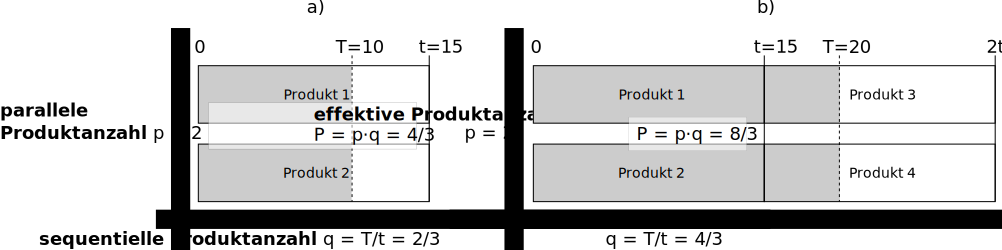
\includegraphics[width=\textwidth]{Produktanzahlen}
	\caption{Veranschaulichung des Zusammenhangs zwischen paralleler, sequentieller und effektiver Produktanzahl. In Fall a) ist der Betrachtungszeitraum $T$ kürzer als die Nutzungsdauer $t$, sodass die zwei parallel eingesetzten Produkte nur anteilig auf das Nutzungssystem angerechnet werden. In Fall b) ist der Betrachtungszeitraum länger als die Nutzungsdauer, sodass zwei Produkte voll und zwei weitere anteilig angerechnet werden.}
	\label{fig:Produktanzahlen}
\end{figure}

%Dies lässt sich mit Gleichung \eqref{eq:t_tech} auch schreiben als:
%\begin{equation}
%	\label{eq:t_Fallunterscheidung}
%	t =\left\{\begin{array}{ll}  t_{\text{max}} & \mbox{falls } t_{\text{max}} < \frac{n_{\text{max}}}{h} \\ \frac{n_{\text{max}}}{h} & \mbox{sonst} \end{array}\right.
%\end{equation} \noteJ{Gleichung \eqref{eq:t_Fallunterscheidung} evt. weglassen}


% b) P = N/n (Annahme: alle Produkte gleiches n)
Der zweite Ansatz zur Bestimmung der effektiven Produktanzahl basiert auf dem Verhältnis zwischen der Nutzungsmenge $n$, die ein einzelnes Produkt während seiner Nutzungsdauer abgibt und der Gesamtnutzungsmenge $N$ des Produktnutzungssystems. Unter der Annahme, dass alle eingesetzten Produkte über die gleiche Nutzungsmenge verfügen, bestimmt sich die effektive Produktanzahl folgendermaßen:
\begin{equation}
P = \frac{N}{n}
\end{equation}

Wir fassen die wichtigsten Ergebnisse dieses Abschnitts als Grundmodell zusammen: \\
\begin{mdframed}[frametitle={Grundmodell}, frametitlerule=true]
	Modellgleichung:
	\begin{equation}
	\label{eq:Grundmodell_MIPS}
	\text{MIPS} = \frac{I}{S}
	\end{equation}
	weitere Grundgleichungen:
	\begin{align}
	I &= I_P + I_N + I_W + I_R + I_\Theta + I_\text{Rest} \label{eq:Grundgleichung_I_1} \\[10pt]
	&= P \cdot i_P + N \cdot i_N + W \cdot i_W + R \cdot i_R + \Theta \cdot i_\Theta + I_\text{Rest} \label{eq:Grundgleichung_I_2}
	\end{align} \\[-35pt]
	\begin{minipage}[t]{0.49\textwidth}
		\begin{align}
		S 	&= S_D = N \cdot A \label{eq:Grundgleichung_S}\\[10pt]
		n &= h \cdot t \label{eq:Grundgleichung_n}
		\end{align}
	\end{minipage}
    \hfill
	\begin{minipage}[t]{0.49\textwidth}
		\begin{align}
		t &= \text{min} \{t_\text{max}, t_\text{tech} := \frac{n_\text{max}}{h}\} \label{eq:Grundgleichung_t} \\
		P &= p \cdot q = p \cdot \frac{T}{t} = \frac{N}{n} \label{eq:Grundgleichung_P}
		\end{align}
	\end{minipage}
\end{mdframed}		
		
		\newpage
\section{Faktor-spezifische Modelle}
\label{sec:Einzeleffekte}
In diesem Abschnitt werden ausgewählte Faktoren für den Umweltverbrauch eines Produktnutzungssystems, die im Zusammenhang mit gemeinschaftlicher Produktnutzung relevant sind, isoliert betrachtet. Wir beginnen mit dem Faktor \enquote{Nutzungshäufigkeit}.

      \subsection{Nutzungshäufigkeit} % Ursprünglich: "Nutzungsdauerverlängerung"
      \label{sec:Nutzungsintensivierung}
      
      Wie bereits im Abschnitt \enquote{\nameref{sec:Grundmodell}} eingeführt, wird mit der Nutzungshäufigkeit $h$ beschrieben, wie häufig ein Produkt pro Zeit genutzt wird. Für eine Waschmaschine wäre dies etwa die Anzahl an Waschgängen pro Woche. Diese Größe ist im Zusammenhang mit gemeinschaftlichen Produktnutzungsformen insofern relevant, als dass ein Produkt typischerweise häufiger genutzt wird, wenn mehrere Personen darauf zugreifen. Daher gehen wir, wie in Tabelle \ref{tab:faktoren_hypothesen} (Abschnitt \ref{sec:Modellierung} \enquote{\nameref{sec:Modellierung}}) formuliert, von der Hypothese einer erhöhten Nutzungshäufigkeit von gemeinschaftlichen Produktnutzungsformen im Vergleich zu herkömmlichen Produktnutzungsformen aus.
      
      Im folgenden Abschnitt wird zunächst ein Modell zum Einfluss der Nutzungshäufigkeit auf die MIPS eines Produktnutzungssystems entwickelt (\enquote{Modellbeschreibung}). Im Anschluss wird dieses Modell angewandt um ein Kriterium für die Reduzierung des Umweltverbrauchs durch eine Erhöhung der Nutzungshäufigkeit abzuleiten (\enquote{Modellanalyse}).
      
      \paragraph{Modellbeschreibung}
      Die Nutzungshäufigkeit steht in engem Zusammenhang zur parallelen Produktanzahl $p$, die ebenfalls im Abschnitt \enquote{\nameref{sec:Grundmodell}} eingeführt wurde: Je weniger Produkte in einem Produktnutzungssystem parallel im Einsatz sind, desto häufiger müssen die einzelnen Produkte genutzt werden um die Service-Nachfrage zu bedienen. Dieser Zusammenhang lässt sich unter Rückgriff auf einige Grundgleichungen aus dem Grundmodell (siehe Nummern über den Gleichheitszeichen) formal folgendermaßen nachvollziehen:
      %
      \begin{equation}
         h \eqnref{eq:Grundgleichung_n} \frac{n}{t} \eqnref{eq:Grundgleichung_P} \frac{\frac{N \cdot t}{p \cdot T}}{t} = \frac{N}{p \cdot T} \eqnref{eq:Grundgleichung_S} \frac{S_D}{A \cdot p \cdot T} \qquad p \in \mathbb{N}
         \label{eq:h(p)_verbose}
      \end{equation}
      %
      Die Nutzungshäufigkeit ist also reziprok proportional zur parallelen Produktanzahl $p$. Da es sich bei $p$ um eine natürliche Zahl handelt und die anderen Größen im vorliegenden Modell als konstant angesehen werden, kann die Nutzungshäufigkeit $h$ nur diskrete Werte annehmen. Dies wird für die Analyse noch von Bedeutung sein.
      
      Wir stellen nun eine Gleichung für die MIPS in Abhängigkeit von der Nutzungshäufigkeit auf. Den Ausgangspunkt bildet die Modellgleichung \eqref{eq:Grundmodell_MIPS} des Grundmodells:
      \begin{equation}
         \text{MIPS} = \frac{I}{S}
      \end{equation}
      %
      Da die Servicemenge durch eine konstante Nachfrage $S=S_D$ gegeben ist, geht es im Folgenden lediglich um die Bestimmung der Material-Inputs $I$. Diese sind gemäß Grundgleichung \eqref{eq:Grundgleichung_I_1} gegeben durch:
      \begin{equation}
         I = I_P + I_N + I_W + I_R + I_\Theta + I_\text{Rest}
      \end{equation}
      %
      Da die produktbezogenen Inputs $I_P$ die einzigen von der Nutzungshäufigkeit abhängigen Material-Inputs sind, fassen wir alle anderen Inputs zu $I_\text{fix}^h$ zusammen:
      \begin{equation}
         I = I_P + I_\text{fix}^h
      \end{equation}
      %
      Mit der Spezifikation der produktbezogenen Inputs $I_P = P \cdot i_P$ gemäß Grundgleichung \eqref{eq:Grundgleichung_I_2} ergibt sich für die MIPS:
      \begin{equation}
         \label{eq:MIPS(h)}
         \text{MIPS}(h) = \frac{I_P + I_\text{fix}^h}{S} = \frac{P(h) \cdot i_P}{S} + \frac{I_\text{fix}^h}{S}
      \end{equation}
      %      
      Die effektive Produktanzahl $P$ ist von der Nutzungshäufigkeit abhängig, wie im folgenden gezeigt wird. Dazu betrachten wir zunächst die Nutzungsdauer $t$. Nach Grundgleichung \eqref{eq:Grundgleichung_t} ist diese folgendermaßen gegeben:
      \begin{equation}
         t = \text{min} \{t_\text{max}, t_\text{tech} := \frac{n_\text{max}}{h}\}
      \end{equation}
      %
      Diese Funktion ist äquivalent zu der folgenden abschnittsweisen Darstellung:
      \begin{equation}
         \label{eq:t(h)}	
         t (h) =\left\{\begin{array}{ll}  t_{\text{max}} & \mbox{falls } h <  \frac{n_{\text{max}}}{t_{\text{max}}} =: h^* \\ \frac{n_{\text{max}}}{h} & \mbox{sonst} \end{array}\right.
      \end{equation}	
      %      
      Dabei ist die Größe $h^* := \frac{n_{\text{max}}}{t_{\text{max}}}$ diejenige Nutzungshäufigkeit, bei der die technische Lebensdauer $t_\text{tech} := \frac{n_\text{max}}{h}$ gleich der Maximalnutzungsdauer $t_\text{max}$ ist. An dieser Stelle wird der Nutzungsvorrat eines Produkts gerade innerhalb der Maximalnutzungsdauer aufgebraucht. Bei einer geringeren Nutzungshäufigkeit ($h<h^*$) ist die Nutzungsdauer durch die konstante Maximalnutzungsdauer gegeben. Bei einer höheren Nutzungshäufigkeit ist hingegen die technische Lebensdauer ausschlaggebend, die mit zunehmender Nutzungshäufigkeit antiproportional abnimmt, da der Nutzungsvorrat schneller aufgebraucht wird (siehe Abbildung \ref{fig:t(h)_n(h)_P(h)} (a)).
      
      \begin{figure}[ht]
         \centering
         % Created by tikzDevice version 0.8.1 on 2015-08-28 10:31:17
% !TEX encoding = UTF-8 Unicode
\begin{tikzpicture}[x=1pt,y=1pt]
\definecolor{fillColor}{RGB}{255,255,255}
\path[use as bounding box,fill=fillColor,fill opacity=0.00] (0,0) rectangle (433.62,180.67);
\begin{scope}
\path[clip] ( 32.47, 48.31) rectangle (127.91,129.19);
\definecolor{drawColor}{RGB}{190,190,190}

\path[draw=drawColor,line width= 0.4pt,line join=round,line cap=round] (124.37, 76.27) --
	(120.55, 77.40) --
	(117.04, 78.53) --
	(113.82, 79.66) --
	(110.84, 80.79) --
	(108.08, 81.92) --
	(105.51, 83.05) --
	(103.12, 84.17) --
	(100.90, 85.30) --
	( 98.81, 86.43) --
	( 96.85, 87.56) --
	( 95.02, 88.69) --
	( 93.29, 89.82) --
	( 91.66, 90.95) --
	( 90.11, 92.08) --
	( 88.66, 93.21) --
	( 87.27, 94.34) --
	( 85.96, 95.46) --
	( 84.72, 96.59) --
	( 83.53, 97.72) --
	( 82.40, 98.85) --
	( 81.33, 99.98) --
	( 80.30,101.11) --
	( 79.32,102.24) --
	( 78.38,103.37) --
	( 77.48,104.50) --
	( 76.62,105.63) --
	( 75.79,106.76) --
	( 75.00,107.88) --
	( 74.23,109.01) --
	( 73.50,110.14) --
	( 72.80,111.27) --
	( 72.12,112.40) --
	( 71.46,113.53) --
	( 70.83,114.66) --
	( 70.22,115.79) --
	( 69.63,116.92) --
	( 69.06,118.05) --
	( 68.51,119.17) --
	( 67.98,120.30) --
	( 67.46,121.43) --
	( 66.97,122.56) --
	( 66.48,123.69) --
	( 66.02,124.82) --
	( 65.56,125.95) --
	( 65.12,126.20) --
	( 64.69,126.20) --
	( 64.28,126.20) --
	( 63.88,126.20) --
	( 63.48,126.20) --
	( 63.10,126.20) --
	( 62.73,126.20) --
	( 62.37,126.20) --
	( 62.02,126.20) --
	( 61.68,126.20) --
	( 61.35,126.20) --
	( 61.02,126.20) --
	( 60.70,126.20) --
	( 60.40,126.20) --
	( 60.10,126.20) --
	( 59.80,126.20) --
	( 59.52,126.20) --
	( 59.24,126.20) --
	( 58.96,126.20) --
	( 58.70,126.20) --
	( 58.44,126.20) --
	( 58.18,126.20) --
	( 57.93,126.20) --
	( 57.69,126.20) --
	( 57.45,126.20) --
	( 57.22,126.20) --
	( 56.99,126.20) --
	( 56.77,126.20) --
	( 56.55,126.20) --
	( 56.34,126.20) --
	( 56.13,126.20) --
	( 55.92,126.20) --
	( 55.72,126.20) --
	( 55.52,126.20) --
	( 55.33,126.20) --
	( 55.14,126.20) --
	( 54.96,126.20) --
	( 54.77,126.20) --
	( 54.60,126.20) --
	( 54.42,126.20) --
	( 54.25,126.20) --
	( 54.08,126.20) --
	( 53.91,126.20) --
	( 53.75,126.20) --
	( 53.59,126.20) --
	( 53.43,126.20) --
	( 53.28,126.20) --
	( 53.13,126.20) --
	( 52.98,126.20) --
	( 52.83,126.20) --
	( 52.69,126.20) --
	( 52.55,126.20) --
	( 52.41,126.20) --
	( 52.27,126.20) --
	( 52.14,126.20) --
	( 52.01,126.20) --
	( 51.88,126.20) --
	( 51.75,126.20) --
	( 51.62,126.20) --
	( 51.50,126.20) --
	( 51.38,126.20) --
	( 51.26,126.20) --
	( 51.14,126.20) --
	( 51.02,126.20) --
	( 50.91,126.20) --
	( 50.80,126.20) --
	( 50.69,126.20) --
	( 50.58,126.20) --
	( 50.47,126.20) --
	( 50.36,126.20) --
	( 50.26,126.20) --
	( 50.15,126.20) --
	( 50.05,126.20) --
	( 49.95,126.20) --
	( 49.85,126.20) --
	( 49.76,126.20) --
	( 49.66,126.20) --
	( 49.56,126.20) --
	( 49.47,126.20) --
	( 49.38,126.20) --
	( 49.29,126.20) --
	( 49.20,126.20) --
	( 49.11,126.20) --
	( 49.02,126.20) --
	( 48.94,126.20) --
	( 48.85,126.20) --
	( 48.77,126.20) --
	( 48.69,126.20) --
	( 48.60,126.20) --
	( 48.52,126.20) --
	( 48.44,126.20) --
	( 48.36,126.20) --
	( 48.29,126.20) --
	( 48.21,126.20) --
	( 48.13,126.20) --
	( 48.06,126.20) --
	( 47.99,126.20) --
	( 47.91,126.20) --
	( 47.84,126.20) --
	( 47.77,126.20) --
	( 47.70,126.20) --
	( 47.63,126.20) --
	( 47.56,126.20) --
	( 47.49,126.20) --
	( 47.43,126.20) --
	( 47.36,126.20) --
	( 47.29,126.20) --
	( 47.23,126.20) --
	( 47.16,126.20) --
	( 47.10,126.20) --
	( 47.04,126.20) --
	( 46.98,126.20) --
	( 46.92,126.20) --
	( 46.85,126.20) --
	( 46.79,126.20) --
	( 46.74,126.20) --
	( 46.68,126.20) --
	( 46.62,126.20) --
	( 46.56,126.20) --
	( 46.51,126.20) --
	( 46.45,126.20) --
	( 46.39,126.20) --
	( 46.34,126.20) --
	( 46.28,126.20) --
	( 46.23,126.20) --
	( 46.18,126.20) --
	( 46.12,126.20) --
	( 46.07,126.20) --
	( 46.02,126.20) --
	( 45.97,126.20) --
	( 45.92,126.20) --
	( 45.87,126.20) --
	( 45.82,126.20) --
	( 45.77,126.20) --
	( 45.72,126.20) --
	( 45.67,126.20) --
	( 45.63,126.20) --
	( 45.58,126.20) --
	( 45.53,126.20) --
	( 45.49,126.20) --
	( 45.44,126.20) --
	( 45.40,126.20) --
	( 45.35,126.20) --
	( 45.31,126.20) --
	( 45.26,126.20) --
	( 45.22,126.20) --
	( 45.18,126.20) --
	( 45.13,126.20) --
	( 45.09,126.20) --
	( 45.05,126.20) --
	( 45.01,126.20) --
	( 44.96,126.20) --
	( 44.92,126.20) --
	( 44.88,126.20) --
	( 44.84,126.20);
\definecolor{drawColor}{RGB}{0,0,0}
\definecolor{fillColor}{RGB}{255,255,255}

\path[draw=drawColor,line width= 0.4pt,line join=round,line cap=round,fill=fillColor] (123.06, 74.96) rectangle (125.69, 77.59);

\path[draw=drawColor,line width= 0.4pt,line join=round,line cap=round,fill=fillColor] ( 78.87, 99.92) rectangle ( 81.51,102.55);

\path[draw=drawColor,line width= 0.4pt,line join=round,line cap=round,fill=fillColor] ( 64.15,124.88) rectangle ( 66.78,127.52);

\path[draw=drawColor,line width= 0.4pt,line join=round,line cap=round,fill=fillColor] ( 56.78,124.88) rectangle ( 59.41,127.52);

\path[draw=drawColor,line width= 0.4pt,line join=round,line cap=round,fill=fillColor] ( 52.36,124.88) rectangle ( 55.00,127.52);

\path[draw=drawColor,line width= 0.4pt,line join=round,line cap=round,fill=fillColor] ( 49.42,124.88) rectangle ( 52.05,127.52);

\path[draw=drawColor,line width= 0.4pt,line join=round,line cap=round,fill=fillColor] ( 47.31,124.88) rectangle ( 49.95,127.52);

\path[draw=drawColor,line width= 0.4pt,line join=round,line cap=round,fill=fillColor] ( 45.74,124.88) rectangle ( 48.37,127.52);

\path[draw=drawColor,line width= 0.4pt,line join=round,line cap=round,fill=fillColor] ( 44.51,124.88) rectangle ( 47.14,127.52);

\path[draw=drawColor,line width= 0.4pt,line join=round,line cap=round,fill=fillColor] ( 43.53,124.88) rectangle ( 46.16,127.52);
\end{scope}
\begin{scope}
\path[clip] (  0.00,  0.00) rectangle (144.54,180.67);
\definecolor{drawColor}{RGB}{0,0,0}

\node[text=drawColor,anchor=base,inner sep=0pt, outer sep=0pt, scale=  0.66] at ( 80.19, 18.22) {Nutzungsh"aufigkeit $h$ [NE/Jahr]};

\node[text=drawColor,rotate= 90.00,anchor=base,inner sep=0pt, outer sep=0pt, scale=  0.66] at (  7.13, 88.75) {Nutzungsdauer $t$ [Jahre]};
\end{scope}
\begin{scope}
\path[clip] ( 32.47, 48.31) rectangle (127.91,129.19);
\definecolor{drawColor}{RGB}{0,0,0}

\path[draw=drawColor,line width= 0.4pt,dash pattern=on 1pt off 3pt ,line join=round,line cap=round] ( 65.46, 48.31) -- ( 65.46,129.19);
\end{scope}
\begin{scope}
\path[clip] (  0.00,  0.00) rectangle (144.54,180.67);
\definecolor{drawColor}{RGB}{0,0,0}

\node[text=drawColor,anchor=base,inner sep=0pt, outer sep=0pt, scale=  0.79] at ( 80.19,164.83) {\bfseries Nutzungsdauer $t(h)$};
\end{scope}
\begin{scope}
\path[clip] (  0.00,  0.00) rectangle (433.62,180.67);
\definecolor{drawColor}{RGB}{0,0,0}

\path[draw=drawColor,line width= 0.4pt,line join=round,line cap=round] ( 36.01, 48.31) -- (124.37, 48.31);

\path[draw=drawColor,line width= 0.4pt,line join=round,line cap=round] ( 36.01, 48.31) -- ( 36.01, 44.35);

\path[draw=drawColor,line width= 0.4pt,line join=round,line cap=round] ( 65.46, 48.31) -- ( 65.46, 44.35);

\path[draw=drawColor,line width= 0.4pt,line join=round,line cap=round] ( 80.19, 48.31) -- ( 80.19, 44.35);

\path[draw=drawColor,line width= 0.4pt,line join=round,line cap=round] (124.37, 48.31) -- (124.37, 44.35);

\node[text=drawColor,anchor=base,inner sep=0pt, outer sep=0pt, scale=  0.66] at ( 36.01, 34.06) {0};

\node[text=drawColor,anchor=base,inner sep=0pt, outer sep=0pt, scale=  0.66] at ( 65.46, 34.06) {$h^*$};

\node[text=drawColor,anchor=base,inner sep=0pt, outer sep=0pt, scale=  0.66] at ( 80.19, 34.06) {500};

\node[text=drawColor,anchor=base,inner sep=0pt, outer sep=0pt, scale=  0.66] at (124.37, 34.06) {1000};

\path[draw=drawColor,line width= 0.4pt,line join=round,line cap=round] ( 32.47, 51.31) -- ( 32.47,126.20);

\path[draw=drawColor,line width= 0.4pt,line join=round,line cap=round] ( 32.47, 51.31) -- ( 28.51, 51.31);

\path[draw=drawColor,line width= 0.4pt,line join=round,line cap=round] ( 32.47, 76.27) -- ( 28.51, 76.27);

\path[draw=drawColor,line width= 0.4pt,line join=round,line cap=round] ( 32.47,101.24) -- ( 28.51,101.24);

\path[draw=drawColor,line width= 0.4pt,line join=round,line cap=round] ( 32.47,126.20) -- ( 28.51,126.20);

\node[text=drawColor,rotate= 90.00,anchor=base,inner sep=0pt, outer sep=0pt, scale=  0.66] at ( 22.97, 51.31) {0};

\node[text=drawColor,rotate= 90.00,anchor=base,inner sep=0pt, outer sep=0pt, scale=  0.66] at ( 22.97, 76.27) {5};

\node[text=drawColor,rotate= 90.00,anchor=base,inner sep=0pt, outer sep=0pt, scale=  0.66] at ( 22.97,101.24) {10};

\node[text=drawColor,rotate= 90.00,anchor=base,inner sep=0pt, outer sep=0pt, scale=  0.66] at ( 22.97,126.20) {15};

\path[draw=drawColor,line width= 0.4pt,line join=round,line cap=round] ( 44.84,129.19) -- (124.37,129.19);

\path[draw=drawColor,line width= 0.4pt,line join=round,line cap=round] ( 44.84,129.19) -- ( 44.84,133.15);

\path[draw=drawColor,line width= 0.4pt,line join=round,line cap=round] ( 45.83,129.19) -- ( 45.83,133.15);

\path[draw=drawColor,line width= 0.4pt,line join=round,line cap=round] ( 47.05,129.19) -- ( 47.05,133.15);

\path[draw=drawColor,line width= 0.4pt,line join=round,line cap=round] ( 48.63,129.19) -- ( 48.63,133.15);

\path[draw=drawColor,line width= 0.4pt,line join=round,line cap=round] ( 50.73,129.19) -- ( 50.73,133.15);

\path[draw=drawColor,line width= 0.4pt,line join=round,line cap=round] ( 53.68,129.19) -- ( 53.68,133.15);

\path[draw=drawColor,line width= 0.4pt,line join=round,line cap=round] ( 58.10,129.19) -- ( 58.10,133.15);

\path[draw=drawColor,line width= 0.4pt,line join=round,line cap=round] ( 65.46,129.19) -- ( 65.46,133.15);

\path[draw=drawColor,line width= 0.4pt,line join=round,line cap=round] ( 80.19,129.19) -- ( 80.19,133.15);

\path[draw=drawColor,line width= 0.4pt,line join=round,line cap=round] (124.37,129.19) -- (124.37,133.15);

\node[text=drawColor,anchor=base,inner sep=0pt, outer sep=0pt, scale=  0.66] at ( 44.84,138.70) {10};

\node[text=drawColor,anchor=base,inner sep=0pt, outer sep=0pt, scale=  0.66] at ( 58.10,138.70) {4};

\node[text=drawColor,anchor=base,inner sep=0pt, outer sep=0pt, scale=  0.66] at ( 80.19,138.70) {2};

\node[text=drawColor,anchor=base,inner sep=0pt, outer sep=0pt, scale=  0.66] at (124.37,138.70) {1};

\path[draw=drawColor,line width= 0.4pt,line join=round,line cap=round] ( 32.47, 48.31) --
	(127.91, 48.31) --
	(127.91,129.19) --
	( 32.47,129.19) --
	( 32.47, 48.31);

\node[text=drawColor,anchor=base,inner sep=0pt, outer sep=0pt, scale=  0.66] at ( 80.19,150.58) {parallele Produktanzahl $p$};

\node[text=drawColor,anchor=base,inner sep=0pt, outer sep=0pt, scale=  1.00] at ( 80.19,  2.38) {(a)};
\end{scope}
\begin{scope}
\path[clip] (177.01, 48.31) rectangle (272.45,129.19);
\definecolor{drawColor}{RGB}{190,190,190}

\path[draw=drawColor,line width= 0.4pt,line join=round,line cap=round] (268.91,126.20) --
	(265.09,126.20) --
	(261.58,126.20) --
	(258.36,126.20) --
	(255.38,126.20) --
	(252.62,126.20) --
	(250.05,126.20) --
	(247.66,126.20) --
	(245.44,126.20) --
	(243.35,126.20) --
	(241.39,126.20) --
	(239.56,126.20) --
	(237.83,126.20) --
	(236.20,126.20) --
	(234.65,126.20) --
	(233.20,126.20) --
	(231.81,126.20) --
	(230.50,126.20) --
	(229.26,126.20) --
	(228.07,126.20) --
	(226.94,126.20) --
	(225.87,126.20) --
	(224.84,126.20) --
	(223.86,126.20) --
	(222.92,126.20) --
	(222.02,126.20) --
	(221.16,126.20) --
	(220.33,126.20) --
	(219.54,126.20) --
	(218.77,126.20) --
	(218.04,126.20) --
	(217.34,126.20) --
	(216.66,126.20) --
	(216.00,126.20) --
	(215.37,126.20) --
	(214.76,126.20) --
	(214.17,126.20) --
	(213.60,126.20) --
	(213.05,126.20) --
	(212.52,126.20) --
	(212.00,126.20) --
	(211.51,126.20) --
	(211.02,126.20) --
	(210.56,126.20) --
	(210.10,126.20) --
	(209.66,125.33) --
	(209.23,124.24) --
	(208.82,123.19) --
	(208.42,122.16) --
	(208.02,121.17) --
	(207.64,120.20) --
	(207.27,119.26) --
	(206.91,118.34) --
	(206.56,117.45) --
	(206.22,116.58) --
	(205.89,115.73) --
	(205.56,114.91) --
	(205.24,114.10) --
	(204.94,113.32) --
	(204.64,112.55) --
	(204.34,111.81) --
	(204.06,111.08) --
	(203.78,110.37) --
	(203.50,109.68) --
	(203.24,109.00) --
	(202.98,108.34) --
	(202.72,107.69) --
	(202.47,107.06) --
	(202.23,106.44) --
	(201.99,105.83) --
	(201.76,105.24) --
	(201.53,104.66) --
	(201.31,104.09) --
	(201.09,103.54) --
	(200.88,103.00) --
	(200.67,102.46) --
	(200.46,101.94) --
	(200.26,101.43) --
	(200.06,100.93) --
	(199.87,100.44) --
	(199.68, 99.96) --
	(199.50, 99.49) --
	(199.31, 99.02) --
	(199.14, 98.57) --
	(198.96, 98.12) --
	(198.79, 97.69) --
	(198.62, 97.26) --
	(198.45, 96.84) --
	(198.29, 96.42) --
	(198.13, 96.02) --
	(197.97, 95.62) --
	(197.82, 95.23) --
	(197.67, 94.84) --
	(197.52, 94.46) --
	(197.37, 94.09) --
	(197.23, 93.73) --
	(197.09, 93.37) --
	(196.95, 93.02) --
	(196.81, 92.67) --
	(196.68, 92.33) --
	(196.55, 91.99) --
	(196.42, 91.66) --
	(196.29, 91.33) --
	(196.16, 91.01) --
	(196.04, 90.70) --
	(195.92, 90.39) --
	(195.80, 90.09) --
	(195.68, 89.78) --
	(195.56, 89.49) --
	(195.45, 89.20) --
	(195.34, 88.91) --
	(195.23, 88.63) --
	(195.12, 88.35) --
	(195.01, 88.08) --
	(194.90, 87.81) --
	(194.80, 87.54) --
	(194.69, 87.28) --
	(194.59, 87.02) --
	(194.49, 86.76) --
	(194.39, 86.51) --
	(194.30, 86.26) --
	(194.20, 86.02) --
	(194.10, 85.78) --
	(194.01, 85.54) --
	(193.92, 85.31) --
	(193.83, 85.08) --
	(193.74, 84.85) --
	(193.65, 84.62) --
	(193.56, 84.40) --
	(193.48, 84.18) --
	(193.39, 83.97) --
	(193.31, 83.75) --
	(193.23, 83.54) --
	(193.14, 83.34) --
	(193.06, 83.13) --
	(192.98, 82.93) --
	(192.90, 82.73) --
	(192.83, 82.53) --
	(192.75, 82.33) --
	(192.67, 82.14) --
	(192.60, 81.95) --
	(192.53, 81.76) --
	(192.45, 81.58) --
	(192.38, 81.40) --
	(192.31, 81.21) --
	(192.24, 81.04) --
	(192.17, 80.86) --
	(192.10, 80.68) --
	(192.03, 80.51) --
	(191.97, 80.34) --
	(191.90, 80.17) --
	(191.83, 80.00) --
	(191.77, 79.84) --
	(191.70, 79.68) --
	(191.64, 79.52) --
	(191.58, 79.36) --
	(191.52, 79.20) --
	(191.46, 79.04) --
	(191.39, 78.89) --
	(191.33, 78.74) --
	(191.28, 78.59) --
	(191.22, 78.44) --
	(191.16, 78.29) --
	(191.10, 78.14) --
	(191.05, 78.00) --
	(190.99, 77.86) --
	(190.93, 77.72) --
	(190.88, 77.58) --
	(190.82, 77.44) --
	(190.77, 77.30) --
	(190.72, 77.17) --
	(190.66, 77.03) --
	(190.61, 76.90) --
	(190.56, 76.77) --
	(190.51, 76.64) --
	(190.46, 76.51) --
	(190.41, 76.38) --
	(190.36, 76.26) --
	(190.31, 76.13) --
	(190.26, 76.01) --
	(190.21, 75.89) --
	(190.17, 75.77) --
	(190.12, 75.65) --
	(190.07, 75.53) --
	(190.03, 75.41) --
	(189.98, 75.29) --
	(189.94, 75.18) --
	(189.89, 75.06) --
	(189.85, 74.95) --
	(189.80, 74.84) --
	(189.76, 74.73) --
	(189.72, 74.62) --
	(189.67, 74.51) --
	(189.63, 74.40) --
	(189.59, 74.29) --
	(189.55, 74.19) --
	(189.50, 74.08) --
	(189.46, 73.98) --
	(189.42, 73.88) --
	(189.38, 73.78);
\definecolor{drawColor}{RGB}{0,0,0}
\definecolor{fillColor}{RGB}{255,255,255}

\path[draw=drawColor,line width= 0.4pt,line join=round,line cap=round,fill=fillColor] (267.60,124.88) rectangle (270.23,127.52);

\path[draw=drawColor,line width= 0.4pt,line join=round,line cap=round,fill=fillColor] (223.41,124.88) rectangle (226.05,127.52);

\path[draw=drawColor,line width= 0.4pt,line join=round,line cap=round,fill=fillColor] (208.69,124.88) rectangle (211.32,127.52);

\path[draw=drawColor,line width= 0.4pt,line join=round,line cap=round,fill=fillColor] (201.32,106.16) rectangle (203.95,108.79);

\path[draw=drawColor,line width= 0.4pt,line join=round,line cap=round,fill=fillColor] (196.90, 94.93) rectangle (199.54, 97.56);

\path[draw=drawColor,line width= 0.4pt,line join=round,line cap=round,fill=fillColor] (193.96, 87.44) rectangle (196.59, 90.07);

\path[draw=drawColor,line width= 0.4pt,line join=round,line cap=round,fill=fillColor] (191.85, 82.09) rectangle (194.49, 84.72);

\path[draw=drawColor,line width= 0.4pt,line join=round,line cap=round,fill=fillColor] (190.28, 78.08) rectangle (192.91, 80.71);

\path[draw=drawColor,line width= 0.4pt,line join=round,line cap=round,fill=fillColor] (189.05, 74.96) rectangle (191.68, 77.59);

\path[draw=drawColor,line width= 0.4pt,line join=round,line cap=round,fill=fillColor] (188.07, 72.46) rectangle (190.70, 75.09);
\end{scope}
\begin{scope}
\path[clip] (144.54,  0.00) rectangle (289.08,180.67);
\definecolor{drawColor}{RGB}{0,0,0}

\node[text=drawColor,anchor=base,inner sep=0pt, outer sep=0pt, scale=  0.66] at (224.73, 18.22) {Nutzungsh"aufigkeit $h$ [NE/Jahr]};

\node[text=drawColor,rotate= 90.00,anchor=base,inner sep=0pt, outer sep=0pt, scale=  0.66] at (151.67, 88.75) {Nutzungsmenge $n$ [NE]};
\end{scope}
\begin{scope}
\path[clip] (177.01, 48.31) rectangle (272.45,129.19);
\definecolor{drawColor}{RGB}{0,0,0}

\path[draw=drawColor,line width= 0.4pt,dash pattern=on 1pt off 3pt ,line join=round,line cap=round] (210.00, 48.31) -- (210.00,129.19);
\end{scope}
\begin{scope}
\path[clip] (144.54,  0.00) rectangle (289.08,180.67);
\definecolor{drawColor}{RGB}{0,0,0}

\node[text=drawColor,anchor=base,inner sep=0pt, outer sep=0pt, scale=  0.79] at (224.73,164.83) {\bfseries Nutzungsmenge $n(h)$};
\end{scope}
\begin{scope}
\path[clip] (  0.00,  0.00) rectangle (433.62,180.67);
\definecolor{drawColor}{RGB}{0,0,0}

\path[draw=drawColor,line width= 0.4pt,line join=round,line cap=round] (180.55, 48.31) -- (268.91, 48.31);

\path[draw=drawColor,line width= 0.4pt,line join=round,line cap=round] (180.55, 48.31) -- (180.55, 44.35);

\path[draw=drawColor,line width= 0.4pt,line join=round,line cap=round] (210.00, 48.31) -- (210.00, 44.35);

\path[draw=drawColor,line width= 0.4pt,line join=round,line cap=round] (224.73, 48.31) -- (224.73, 44.35);

\path[draw=drawColor,line width= 0.4pt,line join=round,line cap=round] (268.91, 48.31) -- (268.91, 44.35);

\node[text=drawColor,anchor=base,inner sep=0pt, outer sep=0pt, scale=  0.66] at (180.55, 34.06) {0};

\node[text=drawColor,anchor=base,inner sep=0pt, outer sep=0pt, scale=  0.66] at (210.00, 34.06) {$h^*$};

\node[text=drawColor,anchor=base,inner sep=0pt, outer sep=0pt, scale=  0.66] at (224.73, 34.06) {500};

\node[text=drawColor,anchor=base,inner sep=0pt, outer sep=0pt, scale=  0.66] at (268.91, 34.06) {1000};

\path[draw=drawColor,line width= 0.4pt,line join=round,line cap=round] (177.01, 51.31) -- (177.01,126.20);

\path[draw=drawColor,line width= 0.4pt,line join=round,line cap=round] (177.01, 51.31) -- (173.05, 51.31);

\path[draw=drawColor,line width= 0.4pt,line join=round,line cap=round] (177.01, 66.29) -- (173.05, 66.29);

\path[draw=drawColor,line width= 0.4pt,line join=round,line cap=round] (177.01, 81.26) -- (173.05, 81.26);

\path[draw=drawColor,line width= 0.4pt,line join=round,line cap=round] (177.01, 96.24) -- (173.05, 96.24);

\path[draw=drawColor,line width= 0.4pt,line join=round,line cap=round] (177.01,111.22) -- (173.05,111.22);

\path[draw=drawColor,line width= 0.4pt,line join=round,line cap=round] (177.01,126.20) -- (173.05,126.20);

\node[text=drawColor,rotate= 90.00,anchor=base,inner sep=0pt, outer sep=0pt, scale=  0.66] at (167.51, 51.31) {0};

\node[text=drawColor,rotate= 90.00,anchor=base,inner sep=0pt, outer sep=0pt, scale=  0.66] at (167.51, 66.29) {1000};

\node[text=drawColor,rotate= 90.00,anchor=base,inner sep=0pt, outer sep=0pt, scale=  0.66] at (167.51, 96.24) {3000};

\node[text=drawColor,rotate= 90.00,anchor=base,inner sep=0pt, outer sep=0pt, scale=  0.66] at (167.51,126.20) {5000};

\path[draw=drawColor,line width= 0.4pt,line join=round,line cap=round] (189.38,129.19) -- (268.91,129.19);

\path[draw=drawColor,line width= 0.4pt,line join=round,line cap=round] (189.38,129.19) -- (189.38,133.15);

\path[draw=drawColor,line width= 0.4pt,line join=round,line cap=round] (190.37,129.19) -- (190.37,133.15);

\path[draw=drawColor,line width= 0.4pt,line join=round,line cap=round] (191.59,129.19) -- (191.59,133.15);

\path[draw=drawColor,line width= 0.4pt,line join=round,line cap=round] (193.17,129.19) -- (193.17,133.15);

\path[draw=drawColor,line width= 0.4pt,line join=round,line cap=round] (195.27,129.19) -- (195.27,133.15);

\path[draw=drawColor,line width= 0.4pt,line join=round,line cap=round] (198.22,129.19) -- (198.22,133.15);

\path[draw=drawColor,line width= 0.4pt,line join=round,line cap=round] (202.64,129.19) -- (202.64,133.15);

\path[draw=drawColor,line width= 0.4pt,line join=round,line cap=round] (210.00,129.19) -- (210.00,133.15);

\path[draw=drawColor,line width= 0.4pt,line join=round,line cap=round] (224.73,129.19) -- (224.73,133.15);

\path[draw=drawColor,line width= 0.4pt,line join=round,line cap=round] (268.91,129.19) -- (268.91,133.15);

\node[text=drawColor,anchor=base,inner sep=0pt, outer sep=0pt, scale=  0.66] at (189.38,138.70) {10};

\node[text=drawColor,anchor=base,inner sep=0pt, outer sep=0pt, scale=  0.66] at (202.64,138.70) {4};

\node[text=drawColor,anchor=base,inner sep=0pt, outer sep=0pt, scale=  0.66] at (224.73,138.70) {2};

\node[text=drawColor,anchor=base,inner sep=0pt, outer sep=0pt, scale=  0.66] at (268.91,138.70) {1};

\path[draw=drawColor,line width= 0.4pt,line join=round,line cap=round] (177.01, 48.31) --
	(272.45, 48.31) --
	(272.45,129.19) --
	(177.01,129.19) --
	(177.01, 48.31);

\node[text=drawColor,anchor=base,inner sep=0pt, outer sep=0pt, scale=  0.66] at (224.73,150.58) {parallele Produktanzahl $p$};

\node[text=drawColor,anchor=base,inner sep=0pt, outer sep=0pt, scale=  1.00] at (224.73,  2.38) {(b)};
\end{scope}
\begin{scope}
\path[clip] (321.55, 48.31) rectangle (416.99,129.19);
\definecolor{drawColor}{RGB}{190,190,190}

\path[draw=drawColor,line width= 0.4pt,line join=round,line cap=round] (413.45, 73.78) --
	(409.63, 73.78) --
	(406.12, 73.78) --
	(402.90, 73.78) --
	(399.92, 73.78) --
	(397.16, 73.78) --
	(394.59, 73.78) --
	(392.20, 73.78) --
	(389.98, 73.78) --
	(387.89, 73.78) --
	(385.93, 73.78) --
	(384.10, 73.78) --
	(382.37, 73.78) --
	(380.74, 73.78) --
	(379.19, 73.78) --
	(377.74, 73.78) --
	(376.35, 73.78) --
	(375.04, 73.78) --
	(373.80, 73.78) --
	(372.61, 73.78) --
	(371.48, 73.78) --
	(370.41, 73.78) --
	(369.38, 73.78) --
	(368.40, 73.78) --
	(367.46, 73.78) --
	(366.56, 73.78) --
	(365.70, 73.78) --
	(364.87, 73.78) --
	(364.08, 73.78) --
	(363.31, 73.78) --
	(362.58, 73.78) --
	(361.88, 73.78) --
	(361.20, 73.78) --
	(360.54, 73.78) --
	(359.91, 73.78) --
	(359.30, 73.78) --
	(358.71, 73.78) --
	(358.14, 73.78) --
	(357.59, 73.78) --
	(357.06, 73.78) --
	(356.54, 73.78) --
	(356.05, 73.78) --
	(355.56, 73.78) --
	(355.10, 73.78) --
	(354.64, 73.78) --
	(354.20, 74.04) --
	(353.77, 74.38) --
	(353.36, 74.72) --
	(352.96, 75.05) --
	(352.56, 75.39) --
	(352.18, 75.73) --
	(351.81, 76.07) --
	(351.45, 76.41) --
	(351.10, 76.75) --
	(350.76, 77.09) --
	(350.43, 77.43) --
	(350.10, 77.76) --
	(349.78, 78.10) --
	(349.48, 78.44) --
	(349.18, 78.78) --
	(348.88, 79.12) --
	(348.60, 79.46) --
	(348.32, 79.80) --
	(348.04, 80.14) --
	(347.78, 80.47) --
	(347.52, 80.81) --
	(347.26, 81.15) --
	(347.01, 81.49) --
	(346.77, 81.83) --
	(346.53, 82.17) --
	(346.30, 82.51) --
	(346.07, 82.84) --
	(345.85, 83.18) --
	(345.63, 83.52) --
	(345.42, 83.86) --
	(345.21, 84.20) --
	(345.00, 84.54) --
	(344.80, 84.88) --
	(344.60, 85.22) --
	(344.41, 85.55) --
	(344.22, 85.89) --
	(344.04, 86.23) --
	(343.85, 86.57) --
	(343.68, 86.91) --
	(343.50, 87.25) --
	(343.33, 87.59) --
	(343.16, 87.93) --
	(342.99, 88.26) --
	(342.83, 88.60) --
	(342.67, 88.94) --
	(342.51, 89.28) --
	(342.36, 89.62) --
	(342.21, 89.96) --
	(342.06, 90.30) --
	(341.91, 90.64) --
	(341.77, 90.97) --
	(341.63, 91.31) --
	(341.49, 91.65) --
	(341.35, 91.99) --
	(341.22, 92.33) --
	(341.09, 92.67) --
	(340.96, 93.01) --
	(340.83, 93.34) --
	(340.70, 93.68) --
	(340.58, 94.02) --
	(340.46, 94.36) --
	(340.34, 94.70) --
	(340.22, 95.04) --
	(340.10, 95.38) --
	(339.99, 95.72) --
	(339.88, 96.05) --
	(339.77, 96.39) --
	(339.66, 96.73) --
	(339.55, 97.07) --
	(339.44, 97.41) --
	(339.34, 97.75) --
	(339.23, 98.09) --
	(339.13, 98.43) --
	(339.03, 98.76) --
	(338.93, 99.10) --
	(338.84, 99.44) --
	(338.74, 99.78) --
	(338.64,100.12) --
	(338.55,100.46) --
	(338.46,100.80) --
	(338.37,101.14) --
	(338.28,101.47) --
	(338.19,101.81) --
	(338.10,102.15) --
	(338.02,102.49) --
	(337.93,102.83) --
	(337.85,103.17) --
	(337.77,103.51) --
	(337.68,103.84) --
	(337.60,104.18) --
	(337.52,104.52) --
	(337.44,104.86) --
	(337.37,105.20) --
	(337.29,105.54) --
	(337.21,105.88) --
	(337.14,106.22) --
	(337.07,106.55) --
	(336.99,106.89) --
	(336.92,107.23) --
	(336.85,107.57) --
	(336.78,107.91) --
	(336.71,108.25) --
	(336.64,108.59) --
	(336.57,108.93) --
	(336.51,109.26) --
	(336.44,109.60) --
	(336.37,109.94) --
	(336.31,110.28) --
	(336.24,110.62) --
	(336.18,110.96) --
	(336.12,111.30) --
	(336.06,111.63) --
	(336.00,111.97) --
	(335.93,112.31) --
	(335.87,112.65) --
	(335.82,112.99) --
	(335.76,113.33) --
	(335.70,113.67) --
	(335.64,114.01) --
	(335.59,114.34) --
	(335.53,114.68) --
	(335.47,115.02) --
	(335.42,115.36) --
	(335.36,115.70) --
	(335.31,116.04) --
	(335.26,116.38) --
	(335.20,116.72) --
	(335.15,117.05) --
	(335.10,117.39) --
	(335.05,117.73) --
	(335.00,118.07) --
	(334.95,118.41) --
	(334.90,118.75) --
	(334.85,119.09) --
	(334.80,119.43) --
	(334.75,119.76) --
	(334.71,120.10) --
	(334.66,120.44) --
	(334.61,120.78) --
	(334.57,121.12) --
	(334.52,121.46) --
	(334.48,121.80) --
	(334.43,122.13) --
	(334.39,122.47) --
	(334.34,122.81) --
	(334.30,123.15) --
	(334.26,123.49) --
	(334.21,123.83) --
	(334.17,124.17) --
	(334.13,124.51) --
	(334.09,124.84) --
	(334.04,125.18) --
	(334.00,125.52) --
	(333.96,125.86) --
	(333.92,126.20);
\definecolor{drawColor}{RGB}{0,0,0}
\definecolor{fillColor}{RGB}{255,255,255}

\path[draw=drawColor,line width= 0.4pt,line join=round,line cap=round,fill=fillColor] (412.14, 72.46) rectangle (414.77, 75.09);

\path[draw=drawColor,line width= 0.4pt,line join=round,line cap=round,fill=fillColor] (367.95, 72.46) rectangle (370.59, 75.09);

\path[draw=drawColor,line width= 0.4pt,line join=round,line cap=round,fill=fillColor] (353.23, 72.46) rectangle (355.86, 75.09);

\path[draw=drawColor,line width= 0.4pt,line join=round,line cap=round,fill=fillColor] (345.86, 79.95) rectangle (348.49, 82.58);

\path[draw=drawColor,line width= 0.4pt,line join=round,line cap=round,fill=fillColor] (341.44, 87.44) rectangle (344.08, 90.07);

\path[draw=drawColor,line width= 0.4pt,line join=round,line cap=round,fill=fillColor] (338.50, 94.93) rectangle (341.13, 97.56);

\path[draw=drawColor,line width= 0.4pt,line join=round,line cap=round,fill=fillColor] (336.39,102.42) rectangle (339.03,105.05);

\path[draw=drawColor,line width= 0.4pt,line join=round,line cap=round,fill=fillColor] (334.82,109.90) rectangle (337.45,112.54);

\path[draw=drawColor,line width= 0.4pt,line join=round,line cap=round,fill=fillColor] (333.59,117.39) rectangle (336.22,120.03);

\path[draw=drawColor,line width= 0.4pt,line join=round,line cap=round,fill=fillColor] (332.61,124.88) rectangle (335.24,127.52);
\end{scope}
\begin{scope}
\path[clip] (289.08,  0.00) rectangle (433.62,180.67);
\definecolor{drawColor}{RGB}{0,0,0}

\node[text=drawColor,anchor=base,inner sep=0pt, outer sep=0pt, scale=  0.66] at (369.27, 18.22) {Nutzungsh"aufigkeit $h$ [NE/Jahr]};

\node[text=drawColor,rotate= 90.00,anchor=base,inner sep=0pt, outer sep=0pt, scale=  0.66] at (296.21, 88.75) {Effektive Produktanzahl $P$};
\end{scope}
\begin{scope}
\path[clip] (321.55, 48.31) rectangle (416.99,129.19);
\definecolor{drawColor}{RGB}{0,0,0}

\path[draw=drawColor,line width= 0.4pt,dash pattern=on 1pt off 3pt ,line join=round,line cap=round] (354.54, 48.31) -- (354.54,129.19);
\end{scope}
\begin{scope}
\path[clip] (289.08,  0.00) rectangle (433.62,180.67);
\definecolor{drawColor}{RGB}{0,0,0}

\node[text=drawColor,anchor=base,inner sep=0pt, outer sep=0pt, scale=  0.79] at (369.27,164.83) {\bfseries Produktanzahl $P(h)$};
\end{scope}
\begin{scope}
\path[clip] (  0.00,  0.00) rectangle (433.62,180.67);
\definecolor{drawColor}{RGB}{0,0,0}

\path[draw=drawColor,line width= 0.4pt,line join=round,line cap=round] (325.09, 48.31) -- (413.45, 48.31);

\path[draw=drawColor,line width= 0.4pt,line join=round,line cap=round] (325.09, 48.31) -- (325.09, 44.35);

\path[draw=drawColor,line width= 0.4pt,line join=round,line cap=round] (354.54, 48.31) -- (354.54, 44.35);

\path[draw=drawColor,line width= 0.4pt,line join=round,line cap=round] (369.27, 48.31) -- (369.27, 44.35);

\path[draw=drawColor,line width= 0.4pt,line join=round,line cap=round] (413.45, 48.31) -- (413.45, 44.35);

\node[text=drawColor,anchor=base,inner sep=0pt, outer sep=0pt, scale=  0.66] at (325.09, 34.06) {0};

\node[text=drawColor,anchor=base,inner sep=0pt, outer sep=0pt, scale=  0.66] at (354.54, 34.06) {$h^*$};

\node[text=drawColor,anchor=base,inner sep=0pt, outer sep=0pt, scale=  0.66] at (369.27, 34.06) {500};

\node[text=drawColor,anchor=base,inner sep=0pt, outer sep=0pt, scale=  0.66] at (413.45, 34.06) {1000};

\path[draw=drawColor,line width= 0.4pt,line join=round,line cap=round] (321.55, 51.31) -- (321.55,118.71);

\path[draw=drawColor,line width= 0.4pt,line join=round,line cap=round] (321.55, 51.31) -- (317.59, 51.31);

\path[draw=drawColor,line width= 0.4pt,line join=round,line cap=round] (321.55, 62.54) -- (317.59, 62.54);

\path[draw=drawColor,line width= 0.4pt,line join=round,line cap=round] (321.55, 73.78) -- (317.59, 73.78);

\path[draw=drawColor,line width= 0.4pt,line join=round,line cap=round] (321.55, 85.01) -- (317.59, 85.01);

\path[draw=drawColor,line width= 0.4pt,line join=round,line cap=round] (321.55, 96.24) -- (317.59, 96.24);

\path[draw=drawColor,line width= 0.4pt,line join=round,line cap=round] (321.55,107.48) -- (317.59,107.48);

\path[draw=drawColor,line width= 0.4pt,line join=round,line cap=round] (321.55,118.71) -- (317.59,118.71);

\node[text=drawColor,rotate= 90.00,anchor=base,inner sep=0pt, outer sep=0pt, scale=  0.66] at (312.05, 51.31) {0};

\node[text=drawColor,rotate= 90.00,anchor=base,inner sep=0pt, outer sep=0pt, scale=  0.66] at (312.05, 62.54) {1};

\node[text=drawColor,rotate= 90.00,anchor=base,inner sep=0pt, outer sep=0pt, scale=  0.66] at (312.05, 73.78) {2};

\node[text=drawColor,rotate= 90.00,anchor=base,inner sep=0pt, outer sep=0pt, scale=  0.66] at (312.05, 85.01) {3};

\node[text=drawColor,rotate= 90.00,anchor=base,inner sep=0pt, outer sep=0pt, scale=  0.66] at (312.05, 96.24) {4};

\node[text=drawColor,rotate= 90.00,anchor=base,inner sep=0pt, outer sep=0pt, scale=  0.66] at (312.05,107.48) {5};

\node[text=drawColor,rotate= 90.00,anchor=base,inner sep=0pt, outer sep=0pt, scale=  0.66] at (312.05,118.71) {6};

\path[draw=drawColor,line width= 0.4pt,line join=round,line cap=round] (333.92,129.19) -- (413.45,129.19);

\path[draw=drawColor,line width= 0.4pt,line join=round,line cap=round] (333.92,129.19) -- (333.92,133.15);

\path[draw=drawColor,line width= 0.4pt,line join=round,line cap=round] (334.91,129.19) -- (334.91,133.15);

\path[draw=drawColor,line width= 0.4pt,line join=round,line cap=round] (336.13,129.19) -- (336.13,133.15);

\path[draw=drawColor,line width= 0.4pt,line join=round,line cap=round] (337.71,129.19) -- (337.71,133.15);

\path[draw=drawColor,line width= 0.4pt,line join=round,line cap=round] (339.81,129.19) -- (339.81,133.15);

\path[draw=drawColor,line width= 0.4pt,line join=round,line cap=round] (342.76,129.19) -- (342.76,133.15);

\path[draw=drawColor,line width= 0.4pt,line join=round,line cap=round] (347.18,129.19) -- (347.18,133.15);

\path[draw=drawColor,line width= 0.4pt,line join=round,line cap=round] (354.54,129.19) -- (354.54,133.15);

\path[draw=drawColor,line width= 0.4pt,line join=round,line cap=round] (369.27,129.19) -- (369.27,133.15);

\path[draw=drawColor,line width= 0.4pt,line join=round,line cap=round] (413.45,129.19) -- (413.45,133.15);

\node[text=drawColor,anchor=base,inner sep=0pt, outer sep=0pt, scale=  0.66] at (333.92,138.70) {10};

\node[text=drawColor,anchor=base,inner sep=0pt, outer sep=0pt, scale=  0.66] at (347.18,138.70) {4};

\node[text=drawColor,anchor=base,inner sep=0pt, outer sep=0pt, scale=  0.66] at (369.27,138.70) {2};

\node[text=drawColor,anchor=base,inner sep=0pt, outer sep=0pt, scale=  0.66] at (413.45,138.70) {1};

\path[draw=drawColor,line width= 0.4pt,line join=round,line cap=round] (321.55, 48.31) --
	(416.99, 48.31) --
	(416.99,129.19) --
	(321.55,129.19) --
	(321.55, 48.31);

\node[text=drawColor,anchor=base,inner sep=0pt, outer sep=0pt, scale=  0.66] at (369.27,150.58) {parallele Produktanzahl $p$};

\node[text=drawColor,anchor=base,inner sep=0pt, outer sep=0pt, scale=  1.00] at (369.27,  2.38) {(c)};
\end{scope}
\end{tikzpicture}

         \caption{Nutzungsdauer, Nutzungsmenge und effektive Produktanzahl in Abhängigkeit von der Nutzungshäufigkeit (untere Skala). Die durchgezogenen Linien folgen dem hypothetischen Funktionsverlauf für eine kontinuierlich angenommene Nutzungshäufigkeit, die kleinen Quadrate zeigen die tatsächlichen Funktionswerte für verschiedene Anzahlen parallel genutzter Produkte (obere Skala). Bei $h^* := \frac{n_{\text{max}}}{t_{\text{max}}}$ wird der Nutzungsvorrat gerade innerhalb der Maximalnutzungsdauer aufgebraucht. Parameter: $N = 10.000$ NE, $n_\text{max} = 5.000$ NE, $T = 10$ Jahre, $t_\text{max} = 15$ Jahre. (NE = Nutzungseinheiten.)}
         \label{fig:t(h)_n(h)_P(h)}
      \end{figure}
      
      Aus Gleichung \eqref{eq:t(h)} lässt sich mit Grundgleichung \eqref{eq:Grundgleichung_n} ein Ausdruck für die Nutzungsmenge $n$ ableiten:
      \begin{equation}
      \label{eq:n(h)_cases}
         n (h) = h \cdot t(h) = \left\{\begin{array}{ll}  h \cdot t_{\text{max}} & \mbox{falls } h < h^* \\ n_{\text{max}} & \mbox{sonst} \end{array}\right.
      \end{equation}	
      %			
      Hier verhält es sich also umgekehrt als bei der Nutzungsdauer: Solange der Nutzungsvorrat innerhalb der Maximalnutzungsdauer aufgrund einer geringen Nutzungshäufigkeit nicht aufgebraucht wird ($h < h^*$), ist die Nutzungsmenge proportional von der Nutzungshäufigkeit abhängig, weil das Produkt in derselben Zeit häufiger genutzt wird: $n (h) = h \cdot t_{\text{max}}$. Bei einer höheren Nutzungshäufigkeit bleibt die Nutzungsmenge hingegen konstant auf dem Niveau des Nutzungsvorrats $n_{\text{max}}$, weil das Produkt nicht darüber hinaus genutzt werden kann (siehe Abbildung \ref{fig:t(h)_n(h)_P(h)} (b)).
      
      Nach diesen Vorüberlegungen kommen wir nun zurück zur Bestimmung der effektiven Produktanzahl. Diese ergibt sich aus den Grundgleichungen \eqref{eq:Grundgleichung_P} und \eqref{eq:Grundgleichung_S}, sowie der soeben hergeleiteten Gleichung \eqref{eq:n(h)_cases}:
      %			
      \begin{equation}
         \label{eq:P(h)}	
         P (h) \eqnref{eq:Grundgleichung_P} \frac{N}{n(h)} \eqnref{eq:Grundgleichung_S} \frac{S}{n(h) \cdot A} \eqnref{eq:n(h)_cases} \left\{\begin{array}{ll}  \frac{S}{A \cdot h \cdot t_{\text{max}}} & \mbox{falls } h < h^* \\[5pt] \frac{S}{A \cdot n_{\text{max}}} & \mbox{sonst} \end{array}\right.
      \end{equation}	
      
      Wiederum ist der Punkt, an dem die Nutzungshäufigkeit gerade so groß ist, dass der Nutzungsvorrat innerhalb der Maximalnutzungsdauer aufgebraucht wird ($h = h^*$), entscheidend: Bei geringerer Nutzungshäufigkeit ist die benötigte Produktanzahl antiproportional zur Nutzungshäufigkeit, bei höherer Nutzungshäufigkeit ist sie hingegen konstant (siehe Abbildung \ref{fig:t(h)_n(h)_P(h)} (c)).

      Es liegen nun alle Voraussetzungen vor um eine Formel für die MIPS in Abhängigkeit von der Nutzungshäufigkeit $h$ aufzustellen. Wir gehen von Gleichung \eqref{eq:MIPS(h)} aus und setzen den eben entwickelten Ausdruck für $P(h)$ ein:
      \begin{equation}
           	\text{MIPS}(h) = \frac{P(h) \cdot i_P}{S} + \frac{I_{\text{fix}}^h}{S} 
           	\eqnref{eq:P(h)} \frac{\frac{S}{n(h) \cdot A} \cdot i_P}{S} + \frac{I_{\text{fix}}^h}{S} = \frac{i_P}{n(h) \cdot A} + \frac{I_{\text{fix}}^h}{S}
      \end{equation}
      %
      Abschließend wenden wir erneut Gleichung \ref{eq:n(h)_cases} an, setzen $S=S_D$ ein und halten das folgende Ergebnis einschließlich der Nebenbedingung aus Gleichung \eqref{eq:h(p)_verbose} fest:
      \\
      
      \begin{mdframed}[frametitle={Nutzungshäufigkeit}, frametitlerule=true]
           	Modell:
           	\begin{align}
           		\text{MIPS}(h) &= \frac{P(h) \cdot i_P}{S_D} + \frac{I_{\text{fix}}^h}{S_D} \label{eq:MIPS(h)_3} \\[10pt]
           		\label{eq:MIPS(h)_2}
           		&= \frac{I_{\text{fix}}^h}{S_D} + \left\{ \begin{array}{ll}  \frac{i_P}{h \cdot t_{\text{max}} \cdot A} & \mbox{falls } h < h^* := \frac{n_{\text{max}}}{t_{\text{max}}} \\[5pt] \frac{i_P}{n_{\text{max}} \cdot A} & \mbox{sonst} \end{array} \right.
           	\end{align}
           	Nebenbedingung:
           	\begin{equation}
           		h = \frac{S_D}{A \cdot p \cdot T} \qquad p \in \mathbb{N}
           		\label{eq:h(p)}
           	\end{equation}
      \end{mdframed}

      \paragraph{Modellanalyse}
      Das Ziel dieser Analyse ist die Ableitung eines Kriteriums zur Senkung des Umweltverbrauchs durch die Erhöhung der Nutzungshäufigkeit. Als Prämisse nehmen wir an, dass sich die Nutzungshäufigkeit von $h^\text{herk}$ bei der herkömmlichen Produktnutzung zu $h^\text{gem}$ bei der gemeinschaftlichen Produktnutzung erhöht. In Abbildung \ref{fig:MIPS(h)} ist der Verlauf der MIPS in Abhängigkeit von $h$ beispielhaft dargestellt, sodass die Analyse grafisch nachvollzogen werden kann.
      
      \begin{figure}[htp]
         \centering
         % Created by tikzDevice version 0.8.1 on 2015-04-03 10:57:13
% !TEX encoding = UTF-8 Unicode
\begin{tikzpicture}[x=1pt,y=1pt]
\definecolor{fillColor}{RGB}{255,255,255}
\path[use as bounding box,fill=fillColor,fill opacity=0.00] (0,0) rectangle (419.17,289.08);
\begin{scope}
\path[clip] ( 46.80, 49.20) rectangle (417.97,221.88);
\definecolor{drawColor}{RGB}{190,190,190}

\path[draw=drawColor,line width= 0.4pt,line join=round,line cap=round] (404.22,108.89) --
	(381.63,108.89) --
	(361.83,108.89) --
	(344.33,108.89) --
	(328.75,108.89) --
	(314.79,108.89) --
	(302.21,108.89) --
	(290.82,108.89) --
	(280.45,108.89) --
	(270.98,108.89) --
	(262.29,108.89) --
	(254.29,108.89) --
	(246.90,108.89) --
	(240.05,108.89) --
	(233.69,108.89) --
	(227.76,108.89) --
	(222.23,108.89) --
	(217.05,108.89) --
	(212.19,108.89) --
	(207.62,108.89) --
	(203.33,108.89) --
	(199.27,108.89) --
	(195.44,108.89) --
	(191.82,108.89) --
	(188.38,108.89) --
	(185.12,108.89) --
	(182.02,108.89) --
	(179.08,108.89) --
	(176.27,108.89) --
	(173.59,109.25) --
	(171.03,109.87) --
	(168.59,110.50) --
	(166.25,111.12) --
	(164.01,111.75) --
	(161.87,112.37) --
	(159.81,113.00) --
	(157.83,113.62) --
	(155.93,114.25) --
	(154.10,114.87) --
	(152.35,115.50) --
	(150.65,116.12) --
	(149.02,116.75) --
	(147.45,117.37) --
	(145.93,118.00) --
	(144.46,118.62) --
	(143.04,119.25) --
	(141.67,119.87) --
	(140.35,120.50) --
	(139.07,121.12) --
	(137.82,121.75) --
	(136.62,122.37) --
	(135.45,123.00) --
	(134.32,123.62) --
	(133.23,124.25) --
	(132.16,124.87) --
	(131.13,125.50) --
	(130.12,126.12) --
	(129.14,126.75) --
	(128.19,127.37) --
	(127.27,128.00) --
	(126.37,128.62) --
	(125.50,129.25) --
	(124.64,129.87) --
	(123.81,130.50) --
	(123.00,131.12) --
	(122.22,131.75) --
	(121.45,132.37) --
	(120.70,133.00) --
	(119.97,133.62) --
	(119.25,134.25) --
	(118.55,134.87) --
	(117.87,135.50) --
	(117.21,136.12) --
	(116.56,136.75) --
	(115.92,137.37) --
	(115.30,138.00) --
	(114.70,138.62) --
	(114.10,139.24) --
	(113.52,139.87) --
	(112.95,140.49) --
	(112.40,141.12) --
	(111.85,141.74) --
	(111.32,142.37) --
	(110.80,142.99) --
	(110.29,143.62) --
	(109.78,144.24) --
	(109.29,144.87) --
	(108.81,145.49) --
	(108.34,146.12) --
	(107.88,146.74) --
	(107.42,147.37) --
	(106.98,147.99) --
	(106.54,148.62) --
	(106.11,149.24) --
	(105.69,149.87) --
	(105.28,150.49) --
	(104.87,151.12) --
	(104.47,151.74) --
	(104.08,152.37) --
	(103.70,152.99) --
	(103.32,153.62) --
	(102.95,154.24) --
	(102.58,154.87) --
	(102.22,155.49) --
	(101.87,156.12) --
	(101.52,156.74) --
	(101.18,157.37) --
	(100.85,157.99) --
	(100.52,158.62) --
	(100.19,159.24) --
	( 99.87,159.87) --
	( 99.56,160.49) --
	( 99.25,161.12) --
	( 98.95,161.74) --
	( 98.65,162.37) --
	( 98.35,162.99) --
	( 98.06,163.62) --
	( 97.78,164.24) --
	( 97.49,164.87) --
	( 97.22,165.49) --
	( 96.94,166.12) --
	( 96.68,166.74) --
	( 96.41,167.37) --
	( 96.15,167.99) --
	( 95.89,168.62) --
	( 95.64,169.24) --
	( 95.39,169.87) --
	( 95.14,170.49) --
	( 94.90,171.12) --
	( 94.66,171.74) --
	( 94.42,172.37) --
	( 94.19,172.99) --
	( 93.96,173.62) --
	( 93.73,174.24) --
	( 93.51,174.86) --
	( 93.29,175.49) --
	( 93.07,176.11) --
	( 92.85,176.74) --
	( 92.64,177.36) --
	( 92.43,177.99) --
	( 92.22,178.61) --
	( 92.02,179.24) --
	( 91.82,179.86) --
	( 91.62,180.49) --
	( 91.42,181.11) --
	( 91.23,181.74) --
	( 91.04,182.36) --
	( 90.85,182.99) --
	( 90.66,183.61) --
	( 90.48,184.24) --
	( 90.29,184.86) --
	( 90.11,185.49) --
	( 89.94,186.11) --
	( 89.76,186.74) --
	( 89.59,187.36) --
	( 89.42,187.99) --
	( 89.25,188.61) --
	( 89.08,189.24) --
	( 88.91,189.86) --
	( 88.75,190.49) --
	( 88.59,191.11) --
	( 88.43,191.74) --
	( 88.27,192.36) --
	( 88.11,192.99) --
	( 87.96,193.61) --
	( 87.81,194.24) --
	( 87.65,194.86) --
	( 87.50,195.49) --
	( 87.36,196.11) --
	( 87.21,196.74) --
	( 87.07,197.36) --
	( 86.92,197.99) --
	( 86.78,198.61) --
	( 86.64,199.24) --
	( 86.50,199.86) --
	( 86.36,200.49) --
	( 86.23,201.11) --
	( 86.09,201.74) --
	( 85.96,202.36) --
	( 85.83,202.99) --
	( 85.70,203.61) --
	( 85.57,204.24) --
	( 85.44,204.86) --
	( 85.32,205.49) --
	( 85.19,206.11) --
	( 85.07,206.74) --
	( 84.95,207.36) --
	( 84.82,207.99) --
	( 84.70,208.61) --
	( 84.59,209.24) --
	( 84.47,209.86) --
	( 84.35,210.49) --
	( 84.24,211.11) --
	( 84.12,211.73) --
	( 84.01,212.36) --
	( 83.90,212.98) --
	( 83.79,213.61) --
	( 83.68,214.23) --
	( 83.57,214.86) --
	( 83.46,215.48);
\definecolor{drawColor}{RGB}{0,0,0}
\definecolor{fillColor}{RGB}{255,255,255}

\path[draw=drawColor,line width= 0.4pt,line join=round,line cap=round,fill=fillColor] (402.23,106.90) rectangle (406.21,110.89);

\path[draw=drawColor,line width= 0.4pt,line join=round,line cap=round,fill=fillColor] (230.39,106.90) rectangle (234.38,110.89);

\path[draw=drawColor,line width= 0.4pt,line join=round,line cap=round,fill=fillColor] (173.11,106.90) rectangle (177.10,110.89);

\path[draw=drawColor,line width= 0.4pt,line join=round,line cap=round,fill=fillColor] (144.47,115.78) rectangle (148.46,119.77);

\path[draw=drawColor,line width= 0.4pt,line join=round,line cap=round,fill=fillColor] (127.29,124.66) rectangle (131.28,128.65);

\path[draw=drawColor,line width= 0.4pt,line join=round,line cap=round,fill=fillColor] (115.83,133.55) rectangle (119.82,137.53);

\path[draw=drawColor,line width= 0.4pt,line join=round,line cap=round,fill=fillColor] (107.65,142.43) rectangle (111.64,146.42);

\path[draw=drawColor,line width= 0.4pt,line join=round,line cap=round,fill=fillColor] (101.51,151.31) rectangle (105.50,155.30);

\path[draw=drawColor,line width= 0.4pt,line join=round,line cap=round,fill=fillColor] ( 96.74,160.19) rectangle (100.73,164.18);

\path[draw=drawColor,line width= 0.4pt,line join=round,line cap=round,fill=fillColor] ( 92.92,169.08) rectangle ( 96.91,173.06);

\path[draw=drawColor,line width= 0.4pt,line join=round,line cap=round,fill=fillColor] ( 89.80,177.96) rectangle ( 93.78,181.95);

\path[draw=drawColor,line width= 0.4pt,line join=round,line cap=round,fill=fillColor] ( 87.19,186.84) rectangle ( 91.18,190.83);

\path[draw=drawColor,line width= 0.4pt,line join=round,line cap=round,fill=fillColor] ( 84.99,195.73) rectangle ( 88.98,199.71);

\path[draw=drawColor,line width= 0.4pt,line join=round,line cap=round,fill=fillColor] ( 83.10,204.61) rectangle ( 87.09,208.60);

\path[draw=drawColor,line width= 0.4pt,line join=round,line cap=round,fill=fillColor] ( 81.46,213.49) rectangle ( 85.45,217.48);
\end{scope}
\begin{scope}
\path[clip] (  0.00,  0.00) rectangle (419.17,289.08);
\definecolor{drawColor}{RGB}{0,0,0}

\node[text=drawColor,anchor=base,inner sep=0pt, outer sep=0pt, scale=  1.00] at (232.38,  3.60) {Nutzungsh"aufigkeit $h$ [Nutzungseinheiten/Jahr]};

\node[text=drawColor,rotate= 90.00,anchor=base,inner sep=0pt, outer sep=0pt, scale=  1.00] at (  8.40,135.54) {MIPS [kg/Service-Einheit]};
\end{scope}
\begin{scope}
\path[clip] ( 46.80, 49.20) rectangle (417.97,221.88);
\definecolor{drawColor}{RGB}{0,0,0}

\path[draw=drawColor,line width= 0.4pt,dash pattern=on 1pt off 3pt ,line join=round,line cap=round] (175.10, 49.20) -- (175.10,221.88);

\path[draw=drawColor,line width= 0.4pt,dash pattern=on 1pt off 3pt ,line join=round,line cap=round] (232.38, 49.20) -- (232.38,221.88);
\end{scope}
\begin{scope}
\path[clip] (  0.00,  0.00) rectangle (419.17,289.08);
\definecolor{drawColor}{RGB}{0,0,0}

\node[text=drawColor,anchor=base,inner sep=0pt, outer sep=0pt, scale=  1.20] at (232.38,275.88) {\bfseries Materialintensit"at pro Service-Einheit MIPS$(h)$};
\end{scope}
\begin{scope}
\path[clip] (  0.00,  0.00) rectangle (419.17,289.08);
\definecolor{drawColor}{RGB}{0,0,0}

\path[draw=drawColor,line width= 0.4pt,line join=round,line cap=round] ( 60.55, 49.20) -- (404.22, 49.20);

\path[draw=drawColor,line width= 0.4pt,line join=round,line cap=round] ( 60.55, 49.20) -- ( 60.55, 43.20);

\path[draw=drawColor,line width= 0.4pt,line join=round,line cap=round] (129.28, 49.20) -- (129.28, 43.20);

\path[draw=drawColor,line width= 0.4pt,line join=round,line cap=round] (175.10, 49.20) -- (175.10, 43.20);

\path[draw=drawColor,line width= 0.4pt,line join=round,line cap=round] (198.02, 49.20) -- (198.02, 43.20);

\path[draw=drawColor,line width= 0.4pt,line join=round,line cap=round] (232.38, 49.20) -- (232.38, 43.20);

\path[draw=drawColor,line width= 0.4pt,line join=round,line cap=round] (266.75, 49.20) -- (266.75, 43.20);

\path[draw=drawColor,line width= 0.4pt,line join=round,line cap=round] (335.48, 49.20) -- (335.48, 43.20);

\path[draw=drawColor,line width= 0.4pt,line join=round,line cap=round] (404.22, 49.20) -- (404.22, 43.20);

\node[text=drawColor,anchor=base,inner sep=0pt, outer sep=0pt, scale=  1.00] at ( 60.55, 27.60) {0};

\node[text=drawColor,anchor=base,inner sep=0pt, outer sep=0pt, scale=  1.00] at (129.28, 27.60) {200};

\node[text=drawColor,anchor=base,inner sep=0pt, outer sep=0pt, scale=  1.00] at (175.10, 27.60) {$h^*$};

\node[text=drawColor,anchor=base,inner sep=0pt, outer sep=0pt, scale=  1.00] at (198.02, 27.60) {400};

\node[text=drawColor,anchor=base,inner sep=0pt, outer sep=0pt, scale=  1.00] at (232.38, 27.60) {$h_\text{max}$};

\node[text=drawColor,anchor=base,inner sep=0pt, outer sep=0pt, scale=  1.00] at (266.75, 27.60) {600};

\node[text=drawColor,anchor=base,inner sep=0pt, outer sep=0pt, scale=  1.00] at (335.48, 27.60) {800};

\node[text=drawColor,anchor=base,inner sep=0pt, outer sep=0pt, scale=  1.00] at (404.22, 27.60) {1000};

\path[draw=drawColor,line width= 0.4pt,line join=round,line cap=round] ( 46.80, 55.60) -- ( 46.80,215.48);

\path[draw=drawColor,line width= 0.4pt,line join=round,line cap=round] ( 46.80, 55.60) -- ( 40.80, 55.60);

\path[draw=drawColor,line width= 0.4pt,line join=round,line cap=round] ( 46.80, 82.24) -- ( 40.80, 82.24);

\path[draw=drawColor,line width= 0.4pt,line join=round,line cap=round] ( 46.80,108.89) -- ( 40.80,108.89);

\path[draw=drawColor,line width= 0.4pt,line join=round,line cap=round] ( 46.80,108.89) -- ( 40.80,108.89);

\path[draw=drawColor,line width= 0.4pt,line join=round,line cap=round] ( 46.80,108.89) -- ( 40.80,108.89);

\path[draw=drawColor,line width= 0.4pt,line join=round,line cap=round] ( 46.80,117.77) -- ( 40.80,117.77);

\path[draw=drawColor,line width= 0.4pt,line join=round,line cap=round] ( 46.80,126.66) -- ( 40.80,126.66);

\path[draw=drawColor,line width= 0.4pt,line join=round,line cap=round] ( 46.80,135.54) -- ( 40.80,135.54);

\path[draw=drawColor,line width= 0.4pt,line join=round,line cap=round] ( 46.80,144.42) -- ( 40.80,144.42);

\path[draw=drawColor,line width= 0.4pt,line join=round,line cap=round] ( 46.80,153.31) -- ( 40.80,153.31);

\path[draw=drawColor,line width= 0.4pt,line join=round,line cap=round] ( 46.80,162.19) -- ( 40.80,162.19);

\path[draw=drawColor,line width= 0.4pt,line join=round,line cap=round] ( 46.80,171.07) -- ( 40.80,171.07);

\path[draw=drawColor,line width= 0.4pt,line join=round,line cap=round] ( 46.80,179.95) -- ( 40.80,179.95);

\path[draw=drawColor,line width= 0.4pt,line join=round,line cap=round] ( 46.80,188.84) -- ( 40.80,188.84);

\path[draw=drawColor,line width= 0.4pt,line join=round,line cap=round] ( 46.80,197.72) -- ( 40.80,197.72);

\path[draw=drawColor,line width= 0.4pt,line join=round,line cap=round] ( 46.80,206.60) -- ( 40.80,206.60);

\path[draw=drawColor,line width= 0.4pt,line join=round,line cap=round] ( 46.80,215.48) -- ( 40.80,215.48);

\node[text=drawColor,rotate= 90.00,anchor=base,inner sep=0pt, outer sep=0pt, scale=  1.00] at ( 32.40, 55.60) {0};

\node[text=drawColor,rotate= 90.00,anchor=base,inner sep=0pt, outer sep=0pt, scale=  1.00] at ( 32.40, 82.24) {1};

\node[text=drawColor,rotate= 90.00,anchor=base,inner sep=0pt, outer sep=0pt, scale=  1.00] at ( 32.40,108.89) {2};

\node[text=drawColor,rotate= 90.00,anchor=base,inner sep=0pt, outer sep=0pt, scale=  1.00] at ( 32.40,135.54) {3};

\node[text=drawColor,rotate= 90.00,anchor=base,inner sep=0pt, outer sep=0pt, scale=  1.00] at ( 32.40,162.19) {4};

\node[text=drawColor,rotate= 90.00,anchor=base,inner sep=0pt, outer sep=0pt, scale=  1.00] at ( 32.40,188.84) {5};

\node[text=drawColor,rotate= 90.00,anchor=base,inner sep=0pt, outer sep=0pt, scale=  1.00] at ( 32.40,215.48) {6};

\path[draw=drawColor,line width= 0.4pt,line join=round,line cap=round] ( 83.46,221.88) -- (404.22,221.88);

\path[draw=drawColor,line width= 0.4pt,line join=round,line cap=round] ( 83.46,221.88) -- ( 83.46,227.88);

\path[draw=drawColor,line width= 0.4pt,line join=round,line cap=round] ( 85.09,221.88) -- ( 85.09,227.88);

\path[draw=drawColor,line width= 0.4pt,line join=round,line cap=round] ( 86.98,221.88) -- ( 86.98,227.88);

\path[draw=drawColor,line width= 0.4pt,line join=round,line cap=round] ( 89.19,221.88) -- ( 89.19,227.88);

\path[draw=drawColor,line width= 0.4pt,line join=round,line cap=round] ( 91.79,221.88) -- ( 91.79,227.88);

\path[draw=drawColor,line width= 0.4pt,line join=round,line cap=round] ( 94.91,221.88) -- ( 94.91,227.88);

\path[draw=drawColor,line width= 0.4pt,line join=round,line cap=round] ( 98.73,221.88) -- ( 98.73,227.88);

\path[draw=drawColor,line width= 0.4pt,line join=round,line cap=round] (103.51,221.88) -- (103.51,227.88);

\path[draw=drawColor,line width= 0.4pt,line join=round,line cap=round] (109.64,221.88) -- (109.64,227.88);

\path[draw=drawColor,line width= 0.4pt,line join=round,line cap=round] (117.83,221.88) -- (117.83,227.88);

\path[draw=drawColor,line width= 0.4pt,line join=round,line cap=round] (129.28,221.88) -- (129.28,227.88);

\path[draw=drawColor,line width= 0.4pt,line join=round,line cap=round] (146.46,221.88) -- (146.46,227.88);

\path[draw=drawColor,line width= 0.4pt,line join=round,line cap=round] (175.10,221.88) -- (175.10,227.88);

\path[draw=drawColor,line width= 0.4pt,line join=round,line cap=round] (232.38,221.88) -- (232.38,227.88);

\path[draw=drawColor,line width= 0.4pt,line join=round,line cap=round] (404.22,221.88) -- (404.22,227.88);

\node[text=drawColor,anchor=base,inner sep=0pt, outer sep=0pt, scale=  1.00] at ( 83.46,236.28) {15};

\node[text=drawColor,anchor=base,inner sep=0pt, outer sep=0pt, scale=  1.00] at (103.51,236.28) {8};

\node[text=drawColor,anchor=base,inner sep=0pt, outer sep=0pt, scale=  1.00] at (117.83,236.28) {6};

\node[text=drawColor,anchor=base,inner sep=0pt, outer sep=0pt, scale=  1.00] at (146.46,236.28) {4};

\node[text=drawColor,anchor=base,inner sep=0pt, outer sep=0pt, scale=  1.00] at (175.10,236.28) {3};

\node[text=drawColor,anchor=base,inner sep=0pt, outer sep=0pt, scale=  1.00] at (232.38,236.28) {2};

\node[text=drawColor,anchor=base,inner sep=0pt, outer sep=0pt, scale=  1.00] at (404.22,236.28) {1};

\path[draw=drawColor,line width= 0.4pt,line join=round,line cap=round] ( 46.80, 49.20) --
	(417.97, 49.20) --
	(417.97,221.88) --
	( 46.80,221.88) --
	( 46.80, 49.20);

\node[text=drawColor,anchor=base,inner sep=0pt, outer sep=0pt, scale=  1.00] at (232.38,254.28) {parallele Produktanzahl $p$};
\end{scope}
\end{tikzpicture}

         \caption{MIPS in Abhängigkeit von der Nutzungshäufigkeit (untere Skala). Die durchgezogenen Linien folgen dem hypothetischen Funktionsverlauf für eine kontinuierlich angenommene Nutzungshäufigkeit, die kleinen Quadrate zeigen die tatsächlichen Funktionswerte für verschiedene Anzahlen parallel genutzter Produkte (obere Skala). Bei $h^* := \frac{n_{\text{max}}}{t_{\text{max}}}$ wird der Nutzungsvorrat gerade innerhalb der Maximalnutzungsdauer aufgebraucht. Parameter: $I_\text{fix}$ = 10.000~kg, $S_D$ = 10.000~SE, $i_P$ = 5.000~kg, $A$ = 1~SE/NE, $T$ = 10~Jahre, $t_\text{max}$ = 15~Jahre, $n_\text{max}$ = 5.000~NE, $p_\text{min}$ = 2 (NE~=Nutzungseinheiten, SE~=~Service-Einheiten).}
         \label{fig:MIPS(h)}
      \end{figure}
      
      Gemäß Nebenbedingung \eqref{eq:h(p)} kann die Nutzungshäufigkeit $h$  nur in diskreten Schritten variiert werden. Wir untersuchen zunächst die Änderung der MIPS von einer gegebenen Nutzungshäufigkeit ($h = h_1$) zur nächstgrößeren ($h = h_2$). Diese ist durch die Verringerung der parallelen Produktanzahl von $p = p_1$ auf $p = p_2$ um den Wert 1 gegeben: 
      \begin{equation}
         \label{eq:delta_p}
         \Delta p = p_2 - p_1 = -1
      \end{equation}
      
      Im Anschluss verallgemeinern wir das Analyse-Ergebnis auf eine beliebige ganzzahlige Verringerung $\Delta p$. Zunächst beginnen wir jedoch mit der Änderung der MIPS für die besprochene Erhöhung der Nutzungshäufigkeit. Nach der Modellgleichung \eqref{eq:MIPS(h)_3} ist diese durch den folgenden Ausdruck gegeben:
      \begin{equation}
      	\label{eq:Delta_MIPS_h_2}
      	\Delta \text{MIPS} = \text{MIPS}(h_2) - \text{MIPS}(h_1) = \frac{i_P}{S_D} \cdot (P(h_2) - P(h_1))
      \end{equation}
      
      Unter Berücksichtigung von Gleichung \eqref{eq:MIPS(h)_2} lässt sich dieser Ausdruck näher bestimmen. Dabei ist die Fallunterscheidung nach $h_1$ bzw. $h_2$ in Bezug auf $h^*$ zu berücksichtigen. Da $h_1 < h_2$ gilt, ergeben sich drei mögliche Fälle.
      
      \underline{Fall 1}: $h_1 < h_2 < h^*$ \\
      Hier wird der Nutzungsvorrat eines einzelnen Produkts sowohl vor, als auch nach der Erhöhung der Nutzungshäufigkeit \emph{nicht} aufgebraucht, bevor die Maximalnutzungsdauer erreicht ist. Für die Änderung der MIPS gilt unter Anwendung von Gleichung \eqref{eq:MIPS(h)_2}:
      %
      \begin{align}
      	\Delta \text{MIPS} &= \text{MIPS}(h_2) - \text{MIPS}(h_1) = \frac{i_P}{t_\text{max} \cdot A} \cdot \left( \frac{1}{h_2} - \frac{1}{h_1} \right) \label{eq:Delta_MIPS_h_1}\\[10pt]
      	&\eqnref{eq:h(p)} \frac{i_P}{t_\text{max} \cdot A} \cdot \frac{A \cdot T}{S_D} \cdot (p_2 - p_1) \eqnref{eq:delta_p} - \frac{i_P \cdot T}{t_\text{max} \cdot S_D} = - \frac{q \cdot i_P}{S_D} \nonumber
      \end{align}
      %
      Im letzten Schritt wurde die Definition $q := \frac{T}{t}$ mit $t =
      t_\text{max}$ (gilt wegen $h_1 < h_2 < h^*$) angewendet. Die obige Analyse
      ergibt, dass die MIPS durch die Erhöhung der Nutzungshäufigkeit im ersten Fall bei der Einsparung eines parallel betriebenen Produkts unabhängig vom Ausgangsniveau um einen konstanten Wert abnimmt. Dabei lässt sich der Zähler $q \cdot i_P$ als die produktbezogenen Inputs des eingesparten parallel eingesetzten Produkts identifizieren, wenn man sich vergegenwärtigt, dass im Betrachtungszeitraum nacheinander $q$ Produkte eingesetzt werden.
      
      Dieses Ergebnis lässt sich in Abbildung \ref{fig:MIPS(h)} nachvollziehen: An den gleichbleibenden vertikalen Abständen der Datenpunkte bis zur Stelle $h = h^*$ ist die konstante Verringerung mit jedem eingesparten Produkt gut erkennbar.
      
      \underline{Fall 2}: $h^* \leq h_1 < h_2$ \\
      Der zweite Fall ist dadurch gegeben, dass der Nutzungsvorrat eines einzelnen Produkts sowohl vor, als auch nach der Erhöhung der Nutzungshäufigkeit spätestens bis zum Erreichen der Maximalnutzungsdauer aufgebraucht wird. Es ergibt sich direkt aus Gleichung \eqref{eq:MIPS(h)_2}:
      %
      \begin{equation}
      	\label{eq:Delta_MIPS_h_2}
      	\Delta \text{MIPS} = \text{MIPS}(h_2) - \text{MIPS}(h_1) = 0
      \end{equation}
      %
      Hier bewirkt eine Erhöhung der Nutzungshäufigkeit also keine Veränderung der MIPS. Dies ist darauf zurückzuführen, dass hier die effektive Produktanzahl $P$ unveränderlich ist (siehe Abbildung \ref{fig:t(h)_n(h)_P(h)} (c)). Es wird also effektiv kein Produkt eingespart.
      
      \underline{Fall 3}: $h_1 < h^* \leq h_2$ \\
      Der dritte Fall stellt den Übergang vom ersten zum dritten Fall dar: Vor der Erhöhung der Nutzungshäufigkeit wird der Nutzungsvorrat eines einzelnen Produkts nicht voll ausgeschöpft, nach der Erhöhung jedoch schon. Für die Veränderung der MIPS gilt nach Gleichung \eqref{eq:MIPS(h)_2}:
      %
      \begin{equation}
      	\label{eq:Delta_MIPS_h_3}
         \Delta \text{MIPS} = \text{MIPS}(h_2) - \text{MIPS}(h_1) = \frac{i_P}{A} \cdot \left( \frac{1}{n_\text{max}} - \frac{1}{h_1 \cdot t_\text{max}} \right)
      \end{equation}
      %
      Dieser Ausdruck ist für sich betrachtet nicht sehr aufschlussreich, kann jedoch nach oben und nach unten abgeschätzt werden. Einerseits ist wegen $h_1 < \frac{n_\text{max}}{t_\text{max}}$ der Klammerausdruck und damit der gesamte Ausdruck negativ, also $\Delta \text{MIPS} < 0$. Andererseits gilt wegen $h_2 \geq \frac{n_\text{max}}{t_\text{max}}$:
      %
      \begin{equation}
      	\label{eq:Delta_MIPS_h_3}
      	\Delta \text{MIPS} = \frac{i_P}{A} \cdot \left( \frac{1}{n_\text{max}} - \frac{1}{h_1 \cdot t_\text{max}} \right) \geq \frac{i_P}{A} \cdot \left( \frac{1}{h_2 \cdot t_\text{max}} - \frac{1}{h_1 \cdot t_\text{max}} \right) \eqnref{eq:Delta_MIPS_h_1} - \frac{q \cdot i_P}{S_D}
      \end{equation}
      %			
      Die Änderung der MIPS bewegt sich im dritten Fall also zwischen den Werten der ersten beiden Fälle und ist auch in diesem Sinne als Übergangsfall zu betrachten: Es findet eine Reduktion der MIPS statt, die allerdings ggf. kleiner ist als im ersten Fall.
      
      \subparagraph{Zwischenfazit}
      Sowohl in Fall 1 als auch in Fall 3 wird eine Reduktion der MIPS durch eine Erhöhung der Nutzungshäufigkeit erzielt. Diese beiden Fälle unterscheiden sich von Fall 2, in dem keine Reduktion erreicht wird, durch die Bedingung $h_1 < h^*$. Das heißt eine Erhöhung der Nutzungshäufigkeit führt genau dann zu einer Reduktion des Umweltverbrauchs, wenn der Nutzungsvorrat eines einzelnen Produkts \emph{vor} der Erhöhung der Nutzungshäufigkeit nicht aufgebraucht wird.
      
      \subparagraph{Verallgemeinerung}
      Im bisherigen Teil der Analyse sind wir von einer Erhöhung der Nutzungshäufigkeit ausgegangen, die der Reduktion um genau ein parallel eingesetztes Produkt entspricht. Im Allgemeinen können beim Übergang von der herkömmlichen zur gemeinschaftlichen Produktnutzung jedoch möglicherweise mehrere parallel eingesetzte Produkte eingespart werden. Das Analyse-Ergebnis wird nun auf diese Situation verallgemeinert.
      
      Eine Erhöhung der Nutzungshäufigkeit von $h^\text{herk}$ nach $h^\text{gem}$ entspricht einer Reduktion der parallelen Produktanzahl $\Delta p = p^\text{gem} - p^\text{herk}$. Diese Reduktion -- eine ganze Zahl -- kann gedanklich in eine Reihe von Reduktionen um den Wert 1 unterteilt werden. In jedem Schritt ist dann die obige Analyse gültig und es trifft jeweils einer der drei besprochenen Fälle zu: Je nach Anwendungsfall kann ggf. für eine Reihe von Schritten Fall 1 zutreffen, dann ggf. für einen Schritt Fall 3 und schließlich ggf. wiederum mehrfach Fall 2.
      
      Sobald wenigstens in einem Schritt Fall 1 oder Fall 3 zutrifft, kommt es zu einer Reduktion der MIPS. Andernfalls wird keine Reduktion erzielt. Zur Überprüfung dieser Bedingung genügt es, den ersten Schritt von $p^\text{herk}$ auf $p^\text{herk} - 1$ zu betrachten. Hier lässt sich nun die im Zwischenfazit formulierte Bedingung anwenden. Sie schreibt sich in diesem Kontext als 
      \begin{equation}
          h^\text{herk} < h^* = \frac{\n{max}}{\t{max}}
          \label{eq:Kriterium_Nutzungshäufigkeit}
      \end{equation} 

      Wir halten dieses Ergebnis verbal als Kriterium fest: \\
      
      \begin{mdframed}[frametitle={Kriterium}, frametitlerule=true]				
         Eine Reduktion des Umweltverbrauchs durch eine Erhöhung der Nutzungshäufigkeit bei gemeinschaftlichen Produktnutzungsformen wird genau dann erzielt, wenn die eingesetzten Produkte herkömmlicherweise nicht bis zum Erreichen ihrer technischen Lebensdauer genutzt werden.
     \end{mdframed}\label{Kriterium:Nutzungshäufigkeit}
      
      % der folgende Text ist noch war bei einem Merge Konflikt mit obigem angezeigt
      % wurden. Welcher ist aktueller=!
      % \subparagraph{Fazit}
      % Die Analyse hat bis hierhin gezeigt, dass eine Nutzungsintensivierung im Sinne einer Erhöhung der Nutzungshäufigkeit im schlechtesten Fall keine Änderung der MIPS, und im besten Fall eine Verringerung der MIPS um einen konstanten Ausdruck mit sich bringt. Es kann also direkt kein schädlicher Effekt auftreten. Die Verringerung wird durch die Einsparung eines der parallel betriebenen Produkte erreicht. Eine solche ist nur möglich, wenn die genutzten Produkte vor der Nutzungsintensivierung noch nicht ihre technische Lebensdauer erreichen.

      \clearpage	
      \subsection{Produktauslastung} % Ursprünglich: "Maximierung der Geräteauslastung"
      \label{sec:Produktauslastung}
      	\paragraph{Modellbeschreibung}
      	Unter dem Begriff \enquote{Produktauslastung}, der bereits im Abschnitt \enquote{Grundmodell} eingeführt wurde, verstehen wir die
      	Intensität, mit der ein Produkt während einer einzelnen Nutzung eingesetzt
      wird. Im Fall einer Waschmaschine entspricht dies dem Gewicht der Beladung
      während eines Waschgangs.
      
      Gemäß der in Tabelle \ref{tab:faktoren_hypothesen} (Abschnitt \ref{sec:Modellierung} \enquote{\nameref{sec:Modellierung}}) formulierten Hypothese gehen wir davon aus, dass die durchschnittliche Produktauslastung bei gemeinschaftlichen Produktnutzungsformen höher ist als bei herkömmlichen Produktnutzungsformen. Am Beispiel des gemeinschaftlichen Waschens kann dies folgendermaßen nachvollzogen werden: Nutzer*innen eines Gemeinschaftskellers verwenden möglicherweise von Zeit zu Zeit gemeinsam eine Waschmaschine, da für bestimmte Waschprogramme individuell nur wenig Wäsche anfällt. Auch in einem Waschsalon ist wegen der höheren Kostentransparenz und des größeren Organisationsaufwands je Waschgang davon auszugehen, dass typischerweise größere Mengen Wäsche auf einmal gewaschen werden.
      
      Wie bereits im Grundmodell eingeführt, bezeichnen wir mit der absoluten Produktauslastung $A$ formal die Service-Menge, die mit einer Nutzungseinheit einhergeht. Besitzt das betrachtete Produkt eine maximale Produktauslastung, die wir als Kapazität $K$ bezeichnen, können wir die relative Produktauslastung $a$ einführen:
		\begin{equation}
   		\label{eq:a(A,K)}
   		A = a \cdot K \qquad a \in \left( 0,1 \right]
		\end{equation}
		%
		So ist beispielsweise eine Waschmaschine, die über eine Kapazität von $K = 7 ~ \frac{\text{kg}}{\text{Waschgang}}$ verfügt und mit $A = 3.5 ~ \frac{\text{kg}}{\text{Waschgang}}$ Wäsche beladen ist, genau zur Hälfte ausgelastet, das heißt $a = 50 \%$.
      
      Wir greifen auf die Nebenbedingung \eqref{eq:h(p)} aus dem Modell zur Nutzungshäufigkeit zurück und setzen den eben eingeführten Ausdruck für die absolute Produktauslastung ein:
      \begin{equation}
         \label{eq:h(a)}
         h = \frac{S_D}{A \cdot p \cdot T} \eqnref{eq:a(A,K)} \frac{S_D}{a \cdot K \cdot p \cdot T} \qquad p \in \mathbb{N}
      \end{equation}
      %
      Anders als im Modell zur Nutzungshäufigkeit kann $a$ in diesem Modell frei gewählt werden. Die Nutzungshäufigkeit $h$ passt sich entsprechend an um die Nebenbedingung zu erfüllen. Beispielsweise müsste eine Waschmaschine, die im Mittel zu 80 Prozent beladen wird durchschnittlich nur halb so häufig benutzt werden wie eine Waschmaschine, die im Mittel zu 40 Prozent ausgelastet ist, um die gleiche Menge an gewaschener Wäsche zur Verfügung zu stellen.
      
      Es geht im Folgenden darum, einen Ausdruck für die MIPS eines Produktnutzungssystems in Abhängigkeit von der (relativen) Produktauslastung $a$ aufzustellen. Wir beginnen mit der Modellgleichung \eqref{eq:Grundmodell_MIPS} aus dem Grundmodell:
      \begin{equation}
         \text{MIPS} = \frac{I}{S}
      \end{equation}

      Die Servicemenge ist durch eine konstante Nachfrage $S=S_D$ gegeben. Für die Material-Inputs $I$ ziehen wir Grundgleichung \eqref{eq:Grundgleichung_I_1} heran:
      \begin{equation}
         I = I_P + I_N + I_W + I_R + I_\Theta + I_\text{Rest}
      \end{equation}
      %
      Wir nehmen nur für die produktbezogenen Inputs $I_P$ sowie für die nutzungsbezogenen Inputs $I_N$ eine Abhängigkeit von der Produktauslastung an und fassen die weiteren Inputs zu $I_\text{fix}^a$ zusammen:
      \begin{equation}
         I = I_P + I_N + I_\text{fix}^a
      \end{equation}
      %      
      Mit den Spezifikationen $I_P = P \cdot i_P$ und $I_N = N \cdot i_N$ gemäß Grundgleichung \eqref{eq:Grundgleichung_I_2} erhalten wir für die MIPS:
      \begin{equation}
         \label{eq:MIPS(a)}
         \text{MIPS}(a) = \frac{I_P + I_N + I_\text{fix}^a}{S_D} = \frac{P(a) \cdot i_P}{S_D} + \frac{N(a) \cdot i_N(a)}{S_D} + \frac{I_\text{fix}^a}{S_D}
      \end{equation}
      %
      Wie durch die Notation von $a$ als Parameter der Funktionen $P(a)$, $N(a)$ und $i_N(a)$ bereits angedeutet, modellieren wir drei Einflüsse der Produktauslastung $a$, die wir im Folgenden näher bestimmen werden.

      Erstens übt die Produktauslastung einen Einfluss auf die Produktnutzungsmenge $N$ aus. Dieser lässt sich durch Umstellen von Grundgleichung \eqref{eq:Grundgleichung_S} nach $N$ und Einsetzen von Gleichung \eqref{eq:a(A,K)} ($A = a \cdot K$) nachvollziehen:
		\begin{equation}
         \label{eq:N_a}
   		N(a) = \frac{S_D}{A} = \frac{S_D}{a \cdot K}
		\end{equation}
      %
      Die Produktnutzungsmenge $N$ ist also reziprok proportional zur Produktauslastung $a$.

      Der zweite Einfluss der Produktauslastung betrifft die Inputs je Produktnutzung $i_N$. Er kommt zustande, wenn der Einsatz an Energie oder anderen Betriebsmitteln von der Produktauslastung abhängig ist. So steigt bei einer Waschmaschine beispielsweise der Bedarf an elektrischer Energie, Wasser und Waschmittel, wenn die Maschine voller beladen wird. Formal kann dieser Zusammenhang durch eine funktionale Abhängigkeit der Inputs je Produktnutzung $i_N$ von der Auslastung $a$ beschrieben werden:
   %
     	\begin{equation}
     		i_N = i_N (a)
     	\end{equation}
   %
     	Wir gehen davon aus, dass eine erhöhte Auslastung mit höheren oder wenigstens gleichbleibenden Inputs je Produktnutzung einhergeht. Das heißt, der Funktionsverlauf von $i_N (a)$ kann als monoton steigend angenommen werden:
   %
     	\begin{equation}
     		\frac{\partial i_N}{\partial a} \geq 0
     	\end{equation}
%
      \begin{figure}[htp]
         \centering
         % Created by tikzDevice version 0.8.1 on 2015-02-27 10:39:16
% !TEX encoding = UTF-8 Unicode
\begin{tikzpicture}[x=1pt,y=1pt]
\definecolor{fillColor}{RGB}{255,255,255}
\path[use as bounding box,fill=fillColor,fill opacity=0.00] (0,0) rectangle (397.48,303.53);
\begin{scope}
\path[clip] ( 49.20, 61.20) rectangle (372.28,254.33);
\definecolor{drawColor}{RGB}{0,0,0}

\path[draw=drawColor,line width= 0.4pt,line join=round,line cap=round] ( 91.08,247.18) --
	( 93.80,235.76) --
	( 96.52,226.05) --
	( 99.24,217.67) --
	(101.96,210.37) --
	(104.68,203.95) --
	(107.40,198.26) --
	(110.12,193.17) --
	(112.84,188.60) --
	(115.56,184.47) --
	(118.28,180.71) --
	(121.00,177.29) --
	(123.72,174.14) --
	(126.44,171.25) --
	(129.16,168.58) --
	(131.87,166.10) --
	(134.59,163.80) --
	(137.31,161.65) --
	(140.03,159.65) --
	(142.75,157.77) --
	(145.47,156.01) --
	(148.19,154.35) --
	(150.91,152.79) --
	(153.63,151.31) --
	(156.35,149.92) --
	(159.07,148.60) --
	(161.79,147.34) --
	(164.51,146.15) --
	(167.23,145.02) --
	(169.95,143.93) --
	(172.67,142.90) --
	(175.39,141.92) --
	(178.11,140.98) --
	(180.83,140.08) --
	(183.55,139.21) --
	(186.27,138.38) --
	(188.99,137.59) --
	(191.71,136.82) --
	(194.43,136.09) --
	(197.14,135.38) --
	(199.86,134.70) --
	(202.58,134.05) --
	(205.30,133.41) --
	(208.02,132.80) --
	(210.74,132.21) --
	(213.46,131.64) --
	(216.18,131.09) --
	(218.90,130.55) --
	(221.62,130.04) --
	(224.34,129.53) --
	(227.06,129.05) --
	(229.78,128.58) --
	(232.50,128.12) --
	(235.22,127.68) --
	(237.94,127.24) --
	(240.66,126.83) --
	(243.38,126.42) --
	(246.10,126.02) --
	(248.82,125.64) --
	(251.54,125.26) --
	(254.26,124.89) --
	(256.98,124.54) --
	(259.69,124.19) --
	(262.41,123.85) --
	(265.13,123.52) --
	(267.85,123.20) --
	(270.57,122.89) --
	(273.29,122.58) --
	(276.01,122.28) --
	(278.73,121.99) --
	(281.45,121.70) --
	(284.17,121.42) --
	(286.89,121.15) --
	(289.61,120.88) --
	(292.33,120.62) --
	(295.05,120.37) --
	(297.77,120.12) --
	(300.49,119.87) --
	(303.21,119.63) --
	(305.93,119.40) --
	(308.65,119.17) --
	(311.37,118.94) --
	(314.09,118.72) --
	(316.81,118.50) --
	(319.53,118.29) --
	(322.24,118.08) --
	(324.96,117.88) --
	(327.68,117.68) --
	(330.40,117.48) --
	(333.12,117.29) --
	(335.84,117.10) --
	(338.56,116.91) --
	(341.28,116.73) --
	(344.00,116.55) --
	(346.72,116.37) --
	(349.44,116.20) --
	(352.16,116.03) --
	(354.88,115.86) --
	(357.60,115.69) --
	(360.32,115.53);
\end{scope}
\begin{scope}
\path[clip] (  0.00,  0.00) rectangle (397.48,303.53);
\definecolor{drawColor}{RGB}{0,0,0}

\path[draw=drawColor,line width= 0.4pt,line join=round,line cap=round] ( 61.17, 61.20) -- (360.32, 61.20);

\path[draw=drawColor,line width= 0.4pt,line join=round,line cap=round] ( 61.17, 61.20) -- ( 61.17, 55.20);

\path[draw=drawColor,line width= 0.4pt,line join=round,line cap=round] (121.00, 61.20) -- (121.00, 55.20);

\path[draw=drawColor,line width= 0.4pt,line join=round,line cap=round] (180.83, 61.20) -- (180.83, 55.20);

\path[draw=drawColor,line width= 0.4pt,line join=round,line cap=round] (240.66, 61.20) -- (240.66, 55.20);

\path[draw=drawColor,line width= 0.4pt,line join=round,line cap=round] (300.49, 61.20) -- (300.49, 55.20);

\path[draw=drawColor,line width= 0.4pt,line join=round,line cap=round] (360.32, 61.20) -- (360.32, 55.20);

\node[text=drawColor,anchor=base,inner sep=0pt, outer sep=0pt, scale=  1.00] at ( 61.17, 39.60) {0.0};

\node[text=drawColor,anchor=base,inner sep=0pt, outer sep=0pt, scale=  1.00] at (121.00, 39.60) {0.2};

\node[text=drawColor,anchor=base,inner sep=0pt, outer sep=0pt, scale=  1.00] at (180.83, 39.60) {0.4};

\node[text=drawColor,anchor=base,inner sep=0pt, outer sep=0pt, scale=  1.00] at (240.66, 39.60) {0.6};

\node[text=drawColor,anchor=base,inner sep=0pt, outer sep=0pt, scale=  1.00] at (300.49, 39.60) {0.8};

\node[text=drawColor,anchor=base,inner sep=0pt, outer sep=0pt, scale=  1.00] at (360.32, 39.60) {1.0};

\path[draw=drawColor,line width= 0.4pt,line join=round,line cap=round] ( 49.20, 68.35) -- ( 49.20,209.88);

\path[draw=drawColor,line width= 0.4pt,line join=round,line cap=round] ( 49.20, 68.35) -- ( 43.20, 68.35);

\path[draw=drawColor,line width= 0.4pt,line join=round,line cap=round] ( 49.20,115.53) -- ( 43.20,115.53);

\path[draw=drawColor,line width= 0.4pt,line join=round,line cap=round] ( 49.20,162.71) -- ( 43.20,162.71);

\path[draw=drawColor,line width= 0.4pt,line join=round,line cap=round] ( 49.20,209.88) -- ( 43.20,209.88);

\node[text=drawColor,rotate= 90.00,anchor=base,inner sep=0pt, outer sep=0pt, scale=  1.00] at ( 34.80, 68.35) {0};

\node[text=drawColor,rotate= 90.00,anchor=base,inner sep=0pt, outer sep=0pt, scale=  1.00] at ( 34.80,115.53) {2};

\node[text=drawColor,rotate= 90.00,anchor=base,inner sep=0pt, outer sep=0pt, scale=  1.00] at ( 34.80,162.71) {4};

\node[text=drawColor,rotate= 90.00,anchor=base,inner sep=0pt, outer sep=0pt, scale=  1.00] at ( 34.80,209.88) {6};

\path[draw=drawColor,line width= 0.4pt,line join=round,line cap=round] ( 49.20, 61.20) --
	(372.28, 61.20) --
	(372.28,254.33) --
	( 49.20,254.33) --
	( 49.20, 61.20);
\end{scope}
\begin{scope}
\path[clip] (  0.00,  0.00) rectangle (397.48,303.53);
\definecolor{drawColor}{RGB}{0,0,0}

\node[text=drawColor,anchor=base,inner sep=0pt, outer sep=0pt, scale=  1.20] at (210.74,274.79) {\bfseries Teilmodell: Erhöhung der Produktauslastung};

\node[text=drawColor,anchor=base,inner sep=0pt, outer sep=0pt, scale=  1.00] at (210.74, 15.60) {Produktauslastung $a$};

\node[text=drawColor,rotate= 90.00,anchor=base,inner sep=0pt, outer sep=0pt, scale=  1.00] at ( 10.80,157.77) {$\text{MIPS}_a$};
\end{scope}
\end{tikzpicture}

         \caption{Effektive Produktanzahl $P$ in Abhängigkeit von der Produktauslastung $a$. Bei $a^*$ wird der Nutzungsvorrat gerade innerhalb der Maximalnutzungsdauer aufgebraucht. Parameter: $S_D$ = 40.000~SE, $K$ = 10~SE/NE, $T$ = 10~Jahre, $t_\text{max}$ = 15~Jahre, $n_\text{max}$ = 5.000~NE, $p$ = 3 (NE~=Nutzungseinheiten, SE~=~Service-Einheiten).}
         \label{fig:P(a)}
      \end{figure}
            
      Drittens hat die Produktauslastung einen Einfluss auf die effektive Produktmenge $P$, die in Abbildung \ref{fig:P(a)} dargestellt wird. Um diesen etwas komplexeren Zusammenhang zu erschließen, beginnen wir mit Grundgleichung \eqref{eq:Grundgleichung_P} und wenden Gleichung \eqref{eq:N_a} an:
      \begin{equation}
         P(a) = \frac{N(a)}{n} \eqnref{eq:N_a} \frac{S_D}{a \cdot K \cdot n}
      \end{equation}
      
      Für $n$ übernehmen wir den im Modell zur Nutzungshäufigkeit entwickelten Ausdruck aus Gleichung \eqref{eq:n(h)_cases} und setzen für $h$ die Nebenbedingung \eqref{eq:h(a)} ein:
      \begin{align}
         n &= h \cdot t = \left\{\begin{array}{ll}  h \cdot t_{\text{max}} & \mbox{falls } h < h^* := \frac{n_\text{max}}{t_\text{max}} \\ n_{\text{max}} & \mbox{sonst} \end{array}\right. \\[10 pt]
         &\eqnref{eq:h(a)} \left\{\begin{array}{ll}  \frac{S_D \cdot t_{\text{max}}}{a \cdot K \cdot p \cdot T} & \mbox{falls } h(a) < h^* \\ n_{\text{max}} & \mbox{sonst} \end{array}\right.
      \end{align}
      
      Damit ergibt sich für die effektive Produktanzahl:
      \begin{equation}
         \label{eq:P(a)}
         P(a) = \frac{S_D}{a \cdot K \cdot n} = \left\{\begin{array}{ll}  \frac{p \cdot T}{t_\text{max}} & \mbox{falls } h(a) < h^* \\[6 pt] \frac{S_D}{a \cdot K \cdot n_{\text{max}}} & \mbox{sonst} \end{array}\right.
      \end{equation}
      
      Die aus dem Modell zur Nutzungshäufigkeit übernommene Bedingung der Fallunterscheidung $h(a) < h^*$, die genau dann erfüllt ist, wenn der Nutzungsvorrat eines Produkts innerhalb der Maximalnutzungsdauer aufgebraucht wird, lässt sich unter Verwendung der Nebenbedingung \eqref{eq:h(a)} auch als explizite Bedingung an $a$ schreiben:
      \begin{equation}
         \label{eq:a*}
         h(a) < h^* := \frac{n_\text{max}}{t_\text{max}} \qquad \Leftrightarrow \qquad a > \frac{S_D \cdot t_\text{max}}{K \cdot p \cdot T \cdot n_\text{max}} =: a^*
      \end{equation}
%
     	Nachdem nun alle Bestandteile der MIPS spezifiziert wurden, stellen wir das Modell auf der Grundlage von Gleichung \eqref{eq:MIPS(a)} und unter Verwendung der Gleichungen \eqref{eq:N_a} und \eqref{eq:P(a)} zusammen:
        \\
% BEGIN_FOLD (Modellerweiterung)
%      Wie bereits im Zusammenhang mit Nebenbedingung \eqref{eq:h(a)} erwähnt, gehen wir bisher davon aus, dass die Nutzungshäufigkeit sich an die Produktauslastung anpasst: Bei steigender Produktauslastung muss die Nutzungshäufigkeit unter sonst gleichen Bedingungen sinken, um dieselbe Servicemenge bereitzustellen. Es ist jedoch auch denkbar, dass die Nutzungshäufigkeit auf dem ursprünglichen Niveau bleibt und stattdessen die Anzahl der parallel eingesetzten Produkte reduziert wird. So könnten beispielsweise zwei Personen, die ursprünglich jeweils eine eigene Waschmaschine nutzten und diese je Waschgang zu 40 Prozent beluden, ihre Wäsche gemeinsam in einer einzigen Maschine waschen, die zu 80 Prozent ausgelastet ist.
%      
%      Dieser Zusammenhang kann formal durch die Umstellung der Nebenbedingung \eqref{eq:h(a)} nach $p$ und einsetzen der herkömmlichen Nutzungshäufigkeit $h = h^\text{herk}$ abgebildet werden:
%      \begin{align}
%         & h = \frac{S_D}{a \cdot K \cdot p \cdot T} \qquad p \in \mathbb{N} \\
%         \Leftrightarrow \quad & p(a) = \left\lceil \frac{S_D}{a \cdot K \cdot h^\text{herk} \cdot T} \right\rceil
%      \end{align}
%      %
%      Die Rundungsklammer ist notwendig, da $p$ nur ganzzahlige Werte annehmen kann. Dies hat zur Konsequenz, dass $h = h^\text{herk}$ nur für die Werte von $a$ gilt, bei denen der Ausdruck in der Rundungsklammer ganzzahlig ist. Für alle anderen Werte gilt $h < h^\text{herk}$. Die parallele Produktzahl $p$ ist durch Konstruktion stets größtmöglich um die Bedingung $h \leq h^\text{herk}$ zu erfüllen.
%      
%      
%     	Zusammenfassend lässt sich das folgende Modell festhalten:
%     	\\
% END_FOLD
     	\begin{mdframed}[frametitle={Produktauslastung}, frametitlerule=true]
     		Modell:
        	\begin{align}
            \text{MIPS}(a) &= \frac{P(a) \cdot i_P}{S_D} + \frac{N(a) \cdot i_N(a)}{S_D} + \frac{I_\text{fix}^a}{S_D} \label{eq:MIPS(a)_2} \\[10 pt]
            &\overset{(\ref{eq:N_a},~\ref{eq:P(a)})}{=} \frac{i_N(a)}{a \cdot K} + \frac{I_\text{fix}^a}{S_D} + \left\{\begin{array}{ll}  \frac{i_P \cdot p \cdot T}{t_\text{max} \cdot S_D} & \mbox{falls } h(a) < h^* \quad \overset{\eqref{eq:a*}}{\Leftrightarrow} \quad a > a^* \label{eq:MIPS(a)_3} \\[6 pt] \frac{i_P}{a \cdot K \cdot n_{\text{max}}} & \mbox{sonst} \end{array}\right. \\[10 pt]
            & \text{mit } a^* := \frac{S_D \cdot t_\text{max}}{K \cdot p \cdot T \cdot n_\text{max}} \label{eq:a*_2}
         \end{align}	
     		Nebenbedingung:
     		\begin{equation}
        	   h(a) = \frac{S_D}{a \cdot K \cdot p \cdot T} \qquad p \in \mathbb{N}, \quad a \in \left( 0,1 \right] \label{eq:h(a)_2} 
     		\end{equation}
     		Funktionseigenschaft:
     		\begin{equation}
            \label{eq:d_i_N_d_a}
           	\frac{\partial i_N}{\partial a} \geq 0
     		\end{equation}
     	\end{mdframed}
      
      \paragraph{Modellanalyse}
      Das Ziel dieser Analyse ist die Ableitung eines Kriteriums zur Senkung des Umweltverbrauchs durch die Erhöhung der Produktauslastung bei gemeinschaftlicher Produktnutzung. Die Grundlage hierfür bildet die Prämisse, dass die Produktauslastung bei einer gemeinschaftlichen Produktnutzung größer ist als bei der herkömmlichen Produktnutzung: $a^\text{gem} > a^\text{herk}$. Es werden zunächst die Auswirkungen einer \emph{marginalen} Erhöhung der Produktauslastung auf die MIPS untersucht. Im Anschluss folgt eine Verallgemeinerung der gewonnenen Erkenntnisse auf eine (mehr als marginale) Erhöhung von $a^\text{herk}$ auf $a^\text{gem}$.
      
      Bevor wir mit der formalen Analyse beginnen, betrachten wir zunächst die
      Modellgleichung unter dem Gesichtspunkt, wie sich eine Erhöhung von $a$
      auf die MIPS auswirkt. Wie in der Modellbeschreibung bereits angesprochen,
      wurden drei Einflüsse der Produktauslastung modelliert: ein Einfluss auf
      die Gesamtnutzungsmenge $N$, auf die Inputs je Produktnutzung $i_N$ und auf die effektive Produktanzahl $P$. Diese finden sich in der Modellgleichung \eqref{eq:MIPS(a)_2} als funktionale Abhängigkeiten von $a$ wieder. Mit Hilfe der näher spezifizierten Gleichung \eqref{eq:MIPS(a)_3} kann bereits abgeschätzt werden, in welche Richtung die einzelnen Einflüsse wirken.
      
      Der erste Summand der Modellgleichung ($\frac{i_N(a)}{a \cdot K}$), der
      nutzungsbezogene Teil der MIPS, beinhaltet zwei gegenläufige Wirkungen:
      Bei einer Erhöhung der Produktauslastung verringert sich einerseits die
      Gesamtnutzungsmenge ($a$ im Nenner), andererseits erhöhen sich die Inputs je Produktnutzung (monoton steigende $i_N$ gemäß Funktionseigenschaft \eqref{eq:d_i_N_d_a}).
      
      Der zweite Summand ist unabhängig von $a$ und spielt daher an dieser Stelle keine Rolle. Der dritte Summand, der produktbezogene Teil der MIPS, ist abhängig von $a$ unterschiedlich definiert. Wir betrachten beide Fälle getrennt voneinander:

      Für kleine Produktauslastungen ($a \leq a^*$ gemäß Gleichung \eqref{eq:a*_2}) gilt in Gleichung \eqref{eq:MIPS(a)_3} der untere Fall. In diesem Bereich führt eine Erhöhung der Produktauslastung zu einer Reduktion der effektiven Produktanzahl (vgl. Abbildung \ref{fig:P(a)}) und damit des produktbezogenen Teils der MIPS. Dies liegt daran, dass in diesem Bereich von $a$ jedes Produkt konstant $n_\text{max}$ Nutzungseinheiten abgibt, die bei einer höheren Auslastung mehr Service generieren, sodass weniger Produkte sequentiell eingesetzt werden müssen um die gleiche Service-Menge bereitzustellen.
      
      Für große Produktauslastungen ($a > a^*$) gilt hingegen der obere Fall in Gleichung \eqref{eq:MIPS(a)_3}. Dieser Ausdruck ist unabhängig von $a$, das heißt eine weitere Erhöhung der Auslastung hat keinen Einfluss auf die effektive Produktanzahl (vgl. Abbildung \ref{fig:P(a)}), sodass der produktbezogene Teil der MIPS hier unveränderlich ist. Der Grund hierfür ist, dass die Nutzungshäufigkeit in diesem Bereich von $a$ im selben Maße abnimmt wie die Produktauslastung zunimmt und ein Produkt somit während der konstanten Nutzungsdauer $t_\text{max}$ stets dieselbe Service-Menge bereitstellt.
      \\
      
      Zusammengefasst kommt es bei einer Erhöhung der Produktauslastung zu einem Trade-off zwischen positiven und negativen Effekten. Dieser wird in der folgenden formalen Analyse untersucht. Der Effekt einer marginalen Erhöhung der Produktauslastung kann durch die Ableitung der MIPS nach $a$ bestimmt werden:
      				%
		\begin{equation}
			\label{eq:d_MIPS_d_a}
			\frac{\partial \MIPS[a]}{\partial a} = \frac{i_N'(a)\cdot a - i_N(a)}{a^2 \cdot K} - \left\{\begin{array}{ll} 0 & \mbox{falls } a > a^* := \frac{S_D \cdot t_\text{max}}{n_\text{max} \cdot K \cdot p \cdot T} \\[5pt] \frac{i_P}{a^2 \cdot K \cdot n_{\text{max}}} & \mbox{sonst} \end{array}\right.
		\end{equation}
      				%
		Es lässt sich nun untersuchen, unter welchen Bedingungen eine marginale Erhöhung der Produktauslastung zu einer Verringerung der MIPS führt. Dazu werden die beiden Fälle $a > a^*$ und $a \leq a^*$ separat behandelt.
      
		\underline{Fall 1:} $a > a^*$

		Dies ist der Fall, in dem der Nutzungsvorrat $n_\text{max}$ aufgrund einer geringen Nutzungshäufigkeit $h$ \emph{nicht} innerhalb der Maximalnutzungsdauer $t_\text{max}$ aufgebraucht wird. Hier gilt nach Gleichung \eqref{eq:d_MIPS_d_a} der folgende Zusammenhang:
		%
		\begin{align}
			\frac{\partial \MIPS[a]}{\partial a} < 0 
			\quad \overset{a, K > 0}{\Leftrightarrow} \quad
         & i_N'(a)\cdot a - i_N(a) < 0 \\
         \quad \Leftrightarrow \quad 
			& \epsilon_{i_N, a} := i'_N(a) \cdot  \frac{a}{i_N(a)} < 1 \label{eq:Elastizitaetsbedingung_1}
		\end{align}
      %
      Eine geringfügige Erhöhung der Produktauslastung führt also im Fall eines
      nicht ausgeschöpften Nutzungsvorrats genau dann zu einer Verringerung der
      MIPS, wenn die Inputs pro Nutzungseinheit $i_N$ unelastisch\footnote{Der
          Begriff der Elastizität wird im \nameref{sec:Anhang} erläutert.} auf die Änderung der Produktauslastung reagiert. Diese Bedingung bedeutet, dass die Inputs pro Nutzungseinheit prozentual weniger stark zunehmen dürfen als die prozentuale Steigerung der Produktauslastung.
      
      Abbildung \ref{fig:i_N(a)_MIPS(a)} stellt beispielhaft die Verläufe der MIPS für eine für alle $a$ elastische und eine für alle $a$ unelastische Funktion $i_N(a)$ dar. Im Bereich $a > a^*$ ist der charakteristische Unterschied gut erkennbar: Bei unelastischen Inputs je Nutzung (linke Teilabbildungen) sinken die MIPS, bei elastischen Inputs je Nutzung (rechte Teilabbildung) steigen sie mit zunehmender Produktauslastung.
      
      \begin{figure}[htp]
         \centering
         % Created by tikzDevice version 0.8.1 on 2015-09-08 10:04:55
% !TEX encoding = UTF-8 Unicode
\begin{tikzpicture}[x=1pt,y=1pt]
\definecolor{fillColor}{RGB}{255,255,255}
\path[use as bounding box,fill=fillColor,fill opacity=0.00] (0,0) rectangle (419.17,289.08);
\begin{scope}
\path[clip] ( 50.80,185.38) rectangle (198.63,244.26);
\definecolor{drawColor}{RGB}{0,0,0}

\path[draw=drawColor,line width= 0.4pt,line join=round,line cap=round] ( 56.27,200.37) --
	( 56.41,200.41) --
	( 56.55,200.45) --
	( 56.68,200.49) --
	( 56.82,200.54) --
	( 56.96,200.58) --
	( 57.09,200.62) --
	( 57.23,200.66) --
	( 57.37,200.70) --
	( 57.50,200.75) --
	( 57.64,200.79) --
	( 57.78,200.83) --
	( 57.92,200.87) --
	( 58.05,200.91) --
	( 58.19,200.95) --
	( 58.33,201.00) --
	( 58.46,201.04) --
	( 58.60,201.08) --
	( 58.74,201.12) --
	( 58.87,201.16) --
	( 59.01,201.20) --
	( 59.15,201.25) --
	( 59.29,201.29) --
	( 59.42,201.33) --
	( 59.56,201.37) --
	( 59.70,201.41) --
	( 59.83,201.46) --
	( 59.97,201.50) --
	( 60.11,201.54) --
	( 60.24,201.58) --
	( 60.38,201.62) --
	( 60.52,201.66) --
	( 60.66,201.71) --
	( 60.79,201.75) --
	( 60.93,201.79) --
	( 61.07,201.83) --
	( 61.20,201.87) --
	( 61.34,201.91) --
	( 61.48,201.96) --
	( 61.61,202.00) --
	( 61.75,202.04) --
	( 61.89,202.08) --
	( 62.03,202.12) --
	( 62.16,202.16) --
	( 62.30,202.21) --
	( 62.44,202.25) --
	( 62.57,202.29) --
	( 62.71,202.33) --
	( 62.85,202.37) --
	( 62.99,202.42) --
	( 63.12,202.46) --
	( 63.26,202.50) --
	( 63.40,202.54) --
	( 63.53,202.58) --
	( 63.67,202.62) --
	( 63.81,202.67) --
	( 63.94,202.71) --
	( 64.08,202.75) --
	( 64.22,202.79) --
	( 64.36,202.83) --
	( 64.49,202.87) --
	( 64.63,202.92) --
	( 64.77,202.96) --
	( 64.90,203.00) --
	( 65.04,203.04) --
	( 65.18,203.08) --
	( 65.31,203.13) --
	( 65.45,203.17) --
	( 65.59,203.21) --
	( 65.73,203.25) --
	( 65.86,203.29) --
	( 66.00,203.33) --
	( 66.14,203.38) --
	( 66.27,203.42) --
	( 66.41,203.46) --
	( 66.55,203.50) --
	( 66.68,203.54) --
	( 66.82,203.58) --
	( 66.96,203.63) --
	( 67.10,203.67) --
	( 67.23,203.71) --
	( 67.37,203.75) --
	( 67.51,203.79) --
	( 67.64,203.83) --
	( 67.78,203.88) --
	( 67.92,203.92) --
	( 68.05,203.96) --
	( 68.19,204.00) --
	( 68.33,204.04) --
	( 68.47,204.09) --
	( 68.60,204.13) --
	( 68.74,204.17) --
	( 68.88,204.21) --
	( 69.01,204.25) --
	( 69.15,204.29) --
	( 69.29,204.34) --
	( 69.42,204.38) --
	( 69.56,204.42) --
	( 69.70,204.46) --
	( 69.84,204.50) --
	( 69.97,204.54) --
	( 70.11,204.59) --
	( 70.25,204.63) --
	( 70.38,204.67) --
	( 70.52,204.71) --
	( 70.66,204.75) --
	( 70.80,204.80) --
	( 70.93,204.84) --
	( 71.07,204.88) --
	( 71.21,204.92) --
	( 71.34,204.96) --
	( 71.48,205.00) --
	( 71.62,205.05) --
	( 71.75,205.09) --
	( 71.89,205.13) --
	( 72.03,205.17) --
	( 72.17,205.21) --
	( 72.30,205.25) --
	( 72.44,205.30) --
	( 72.58,205.34) --
	( 72.71,205.38) --
	( 72.85,205.42) --
	( 72.99,205.46) --
	( 73.12,205.51) --
	( 73.26,205.55) --
	( 73.40,205.59) --
	( 73.54,205.63) --
	( 73.67,205.67) --
	( 73.81,205.71) --
	( 73.95,205.76) --
	( 74.08,205.80) --
	( 74.22,205.84) --
	( 74.36,205.88) --
	( 74.49,205.92) --
	( 74.63,205.96) --
	( 74.77,206.01) --
	( 74.91,206.05) --
	( 75.04,206.09) --
	( 75.18,206.13) --
	( 75.32,206.17) --
	( 75.45,206.21) --
	( 75.59,206.26) --
	( 75.73,206.30) --
	( 75.86,206.34) --
	( 76.00,206.38) --
	( 76.14,206.42) --
	( 76.28,206.47) --
	( 76.41,206.51) --
	( 76.55,206.55) --
	( 76.69,206.59) --
	( 76.82,206.63) --
	( 76.96,206.67) --
	( 77.10,206.72) --
	( 77.23,206.76) --
	( 77.37,206.80) --
	( 77.51,206.84) --
	( 77.65,206.88) --
	( 77.78,206.92) --
	( 77.92,206.97) --
	( 78.06,207.01) --
	( 78.19,207.05) --
	( 78.33,207.09) --
	( 78.47,207.13) --
	( 78.61,207.18) --
	( 78.74,207.22) --
	( 78.88,207.26) --
	( 79.02,207.30) --
	( 79.15,207.34) --
	( 79.29,207.38) --
	( 79.43,207.43) --
	( 79.56,207.47) --
	( 79.70,207.51) --
	( 79.84,207.55) --
	( 79.98,207.59) --
	( 80.11,207.63) --
	( 80.25,207.68) --
	( 80.39,207.72) --
	( 80.52,207.76) --
	( 80.66,207.80) --
	( 80.80,207.84) --
	( 80.93,207.88) --
	( 81.07,207.93) --
	( 81.21,207.97) --
	( 81.35,208.01) --
	( 81.48,208.05) --
	( 81.62,208.09) --
	( 81.76,208.14) --
	( 81.89,208.18) --
	( 82.03,208.22) --
	( 82.17,208.26) --
	( 82.30,208.30) --
	( 82.44,208.34) --
	( 82.58,208.39) --
	( 82.72,208.43) --
	( 82.85,208.47) --
	( 82.99,208.51) --
	( 83.13,208.55) --
	( 83.26,208.59) --
	( 83.40,208.64) --
	( 83.54,208.68) --
	( 83.67,208.72) --
	( 83.81,208.76) --
	( 83.95,208.80) --
	( 84.09,208.85) --
	( 84.22,208.89) --
	( 84.36,208.93) --
	( 84.50,208.97) --
	( 84.63,209.01) --
	( 84.77,209.05) --
	( 84.91,209.10) --
	( 85.04,209.14) --
	( 85.18,209.18) --
	( 85.32,209.22) --
	( 85.46,209.26) --
	( 85.59,209.30) --
	( 85.73,209.35) --
	( 85.87,209.39) --
	( 86.00,209.43) --
	( 86.14,209.47) --
	( 86.28,209.51) --
	( 86.42,209.55) --
	( 86.55,209.60) --
	( 86.69,209.64) --
	( 86.83,209.68) --
	( 86.96,209.72) --
	( 87.10,209.76) --
	( 87.24,209.81) --
	( 87.37,209.85) --
	( 87.51,209.89) --
	( 87.65,209.93) --
	( 87.79,209.97) --
	( 87.92,210.01) --
	( 88.06,210.06) --
	( 88.20,210.10) --
	( 88.33,210.14) --
	( 88.47,210.18) --
	( 88.61,210.22) --
	( 88.74,210.26) --
	( 88.88,210.31) --
	( 89.02,210.35) --
	( 89.16,210.39) --
	( 89.29,210.43) --
	( 89.43,210.47) --
	( 89.57,210.52) --
	( 89.70,210.56) --
	( 89.84,210.60) --
	( 89.98,210.64) --
	( 90.11,210.68) --
	( 90.25,210.72) --
	( 90.39,210.77) --
	( 90.53,210.81) --
	( 90.66,210.85) --
	( 90.80,210.89) --
	( 90.94,210.93) --
	( 91.07,210.97) --
	( 91.21,211.02) --
	( 91.35,211.06) --
	( 91.48,211.10) --
	( 91.62,211.14) --
	( 91.76,211.18) --
	( 91.90,211.22) --
	( 92.03,211.27) --
	( 92.17,211.31) --
	( 92.31,211.35) --
	( 92.44,211.39) --
	( 92.58,211.43) --
	( 92.72,211.48) --
	( 92.85,211.52) --
	( 92.99,211.56) --
	( 93.13,211.60) --
	( 93.27,211.64) --
	( 93.40,211.68) --
	( 93.54,211.73) --
	( 93.68,211.77) --
	( 93.81,211.81) --
	( 93.95,211.85) --
	( 94.09,211.89) --
	( 94.23,211.93) --
	( 94.36,211.98) --
	( 94.50,212.02) --
	( 94.64,212.06) --
	( 94.77,212.10) --
	( 94.91,212.14) --
	( 95.05,212.19) --
	( 95.18,212.23) --
	( 95.32,212.27) --
	( 95.46,212.31) --
	( 95.60,212.35) --
	( 95.73,212.39) --
	( 95.87,212.44) --
	( 96.01,212.48) --
	( 96.14,212.52) --
	( 96.28,212.56) --
	( 96.42,212.60) --
	( 96.55,212.64) --
	( 96.69,212.69) --
	( 96.83,212.73) --
	( 96.97,212.77) --
	( 97.10,212.81) --
	( 97.24,212.85) --
	( 97.38,212.89) --
	( 97.51,212.94) --
	( 97.65,212.98) --
	( 97.79,213.02) --
	( 97.92,213.06) --
	( 98.06,213.10) --
	( 98.20,213.15) --
	( 98.34,213.19) --
	( 98.47,213.23) --
	( 98.61,213.27) --
	( 98.75,213.31) --
	( 98.88,213.35) --
	( 99.02,213.40) --
	( 99.16,213.44) --
	( 99.29,213.48) --
	( 99.43,213.52) --
	( 99.57,213.56) --
	( 99.71,213.60) --
	( 99.84,213.65) --
	( 99.98,213.69) --
	(100.12,213.73) --
	(100.25,213.77) --
	(100.39,213.81) --
	(100.53,213.86) --
	(100.66,213.90) --
	(100.80,213.94) --
	(100.94,213.98) --
	(101.08,214.02) --
	(101.21,214.06) --
	(101.35,214.11) --
	(101.49,214.15) --
	(101.62,214.19) --
	(101.76,214.23) --
	(101.90,214.27) --
	(102.04,214.31) --
	(102.17,214.36) --
	(102.31,214.40) --
	(102.45,214.44) --
	(102.58,214.48) --
	(102.72,214.52) --
	(102.86,214.57) --
	(102.99,214.61) --
	(103.13,214.65) --
	(103.27,214.69) --
	(103.41,214.73) --
	(103.54,214.77) --
	(103.68,214.82) --
	(103.82,214.86) --
	(103.95,214.90) --
	(104.09,214.94) --
	(104.23,214.98) --
	(104.36,215.02) --
	(104.50,215.07) --
	(104.64,215.11) --
	(104.78,215.15) --
	(104.91,215.19) --
	(105.05,215.23) --
	(105.19,215.27) --
	(105.32,215.32) --
	(105.46,215.36) --
	(105.60,215.40) --
	(105.73,215.44) --
	(105.87,215.48) --
	(106.01,215.53) --
	(106.15,215.57) --
	(106.28,215.61) --
	(106.42,215.65) --
	(106.56,215.69) --
	(106.69,215.73) --
	(106.83,215.78) --
	(106.97,215.82) --
	(107.10,215.86) --
	(107.24,215.90) --
	(107.38,215.94) --
	(107.52,215.98) --
	(107.65,216.03) --
	(107.79,216.07) --
	(107.93,216.11) --
	(108.06,216.15) --
	(108.20,216.19) --
	(108.34,216.24) --
	(108.47,216.28) --
	(108.61,216.32) --
	(108.75,216.36) --
	(108.89,216.40) --
	(109.02,216.44) --
	(109.16,216.49) --
	(109.30,216.53) --
	(109.43,216.57) --
	(109.57,216.61) --
	(109.71,216.65) --
	(109.85,216.69) --
	(109.98,216.74) --
	(110.12,216.78) --
	(110.26,216.82) --
	(110.39,216.86) --
	(110.53,216.90) --
	(110.67,216.94) --
	(110.80,216.99) --
	(110.94,217.03) --
	(111.08,217.07) --
	(111.22,217.11) --
	(111.35,217.15) --
	(111.49,217.20) --
	(111.63,217.24) --
	(111.76,217.28) --
	(111.90,217.32) --
	(112.04,217.36) --
	(112.17,217.40) --
	(112.31,217.45) --
	(112.45,217.49) --
	(112.59,217.53) --
	(112.72,217.57) --
	(112.86,217.61) --
	(113.00,217.65) --
	(113.13,217.70) --
	(113.27,217.74) --
	(113.41,217.78) --
	(113.54,217.82) --
	(113.68,217.86) --
	(113.82,217.91) --
	(113.96,217.95) --
	(114.09,217.99) --
	(114.23,218.03) --
	(114.37,218.07) --
	(114.50,218.11) --
	(114.64,218.16) --
	(114.78,218.20) --
	(114.91,218.24) --
	(115.05,218.28) --
	(115.19,218.32) --
	(115.33,218.36) --
	(115.46,218.41) --
	(115.60,218.45) --
	(115.74,218.49) --
	(115.87,218.53) --
	(116.01,218.57) --
	(116.15,218.61) --
	(116.28,218.66) --
	(116.42,218.70) --
	(116.56,218.74) --
	(116.70,218.78) --
	(116.83,218.82) --
	(116.97,218.87) --
	(117.11,218.91) --
	(117.24,218.95) --
	(117.38,218.99) --
	(117.52,219.03) --
	(117.66,219.07) --
	(117.79,219.12) --
	(117.93,219.16) --
	(118.07,219.20) --
	(118.20,219.24) --
	(118.34,219.28) --
	(118.48,219.32) --
	(118.61,219.37) --
	(118.75,219.41) --
	(118.89,219.45) --
	(119.03,219.49) --
	(119.16,219.53) --
	(119.30,219.58) --
	(119.44,219.62) --
	(119.57,219.66) --
	(119.71,219.70) --
	(119.85,219.74) --
	(119.98,219.78) --
	(120.12,219.83) --
	(120.26,219.87) --
	(120.40,219.91) --
	(120.53,219.95) --
	(120.67,219.99) --
	(120.81,220.03) --
	(120.94,220.08) --
	(121.08,220.12) --
	(121.22,220.16) --
	(121.35,220.20) --
	(121.49,220.24) --
	(121.63,220.28) --
	(121.77,220.33) --
	(121.90,220.37) --
	(122.04,220.41) --
	(122.18,220.45) --
	(122.31,220.49) --
	(122.45,220.54) --
	(122.59,220.58) --
	(122.72,220.62) --
	(122.86,220.66) --
	(123.00,220.70) --
	(123.14,220.74) --
	(123.27,220.79) --
	(123.41,220.83) --
	(123.55,220.87) --
	(123.68,220.91) --
	(123.82,220.95) --
	(123.96,220.99) --
	(124.09,221.04) --
	(124.23,221.08) --
	(124.37,221.12) --
	(124.51,221.16) --
	(124.64,221.20) --
	(124.78,221.25) --
	(124.92,221.29) --
	(125.05,221.33) --
	(125.19,221.37) --
	(125.33,221.41) --
	(125.47,221.45) --
	(125.60,221.50) --
	(125.74,221.54) --
	(125.88,221.58) --
	(126.01,221.62) --
	(126.15,221.66) --
	(126.29,221.70) --
	(126.42,221.75) --
	(126.56,221.79) --
	(126.70,221.83) --
	(126.84,221.87) --
	(126.97,221.91) --
	(127.11,221.96) --
	(127.25,222.00) --
	(127.38,222.04) --
	(127.52,222.08) --
	(127.66,222.12) --
	(127.79,222.16) --
	(127.93,222.21) --
	(128.07,222.25) --
	(128.21,222.29) --
	(128.34,222.33) --
	(128.48,222.37) --
	(128.62,222.41) --
	(128.75,222.46) --
	(128.89,222.50) --
	(129.03,222.54) --
	(129.16,222.58) --
	(129.30,222.62) --
	(129.44,222.66) --
	(129.58,222.71) --
	(129.71,222.75) --
	(129.85,222.79) --
	(129.99,222.83) --
	(130.12,222.87) --
	(130.26,222.92) --
	(130.40,222.96) --
	(130.53,223.00) --
	(130.67,223.04) --
	(130.81,223.08) --
	(130.95,223.12) --
	(131.08,223.17) --
	(131.22,223.21) --
	(131.36,223.25) --
	(131.49,223.29) --
	(131.63,223.33) --
	(131.77,223.37) --
	(131.90,223.42) --
	(132.04,223.46) --
	(132.18,223.50) --
	(132.32,223.54) --
	(132.45,223.58) --
	(132.59,223.63) --
	(132.73,223.67) --
	(132.86,223.71) --
	(133.00,223.75) --
	(133.14,223.79) --
	(133.28,223.83) --
	(133.41,223.88) --
	(133.55,223.92) --
	(133.69,223.96) --
	(133.82,224.00) --
	(133.96,224.04) --
	(134.10,224.08) --
	(134.23,224.13) --
	(134.37,224.17) --
	(134.51,224.21) --
	(134.65,224.25) --
	(134.78,224.29) --
	(134.92,224.33) --
	(135.06,224.38) --
	(135.19,224.42) --
	(135.33,224.46) --
	(135.47,224.50) --
	(135.60,224.54) --
	(135.74,224.59) --
	(135.88,224.63) --
	(136.02,224.67) --
	(136.15,224.71) --
	(136.29,224.75) --
	(136.43,224.79) --
	(136.56,224.84) --
	(136.70,224.88) --
	(136.84,224.92) --
	(136.97,224.96) --
	(137.11,225.00) --
	(137.25,225.04) --
	(137.39,225.09) --
	(137.52,225.13) --
	(137.66,225.17) --
	(137.80,225.21) --
	(137.93,225.25) --
	(138.07,225.30) --
	(138.21,225.34) --
	(138.34,225.38) --
	(138.48,225.42) --
	(138.62,225.46) --
	(138.76,225.50) --
	(138.89,225.55) --
	(139.03,225.59) --
	(139.17,225.63) --
	(139.30,225.67) --
	(139.44,225.71) --
	(139.58,225.75) --
	(139.71,225.80) --
	(139.85,225.84) --
	(139.99,225.88) --
	(140.13,225.92) --
	(140.26,225.96) --
	(140.40,226.00) --
	(140.54,226.05) --
	(140.67,226.09) --
	(140.81,226.13) --
	(140.95,226.17) --
	(141.09,226.21) --
	(141.22,226.26) --
	(141.36,226.30) --
	(141.50,226.34) --
	(141.63,226.38) --
	(141.77,226.42) --
	(141.91,226.46) --
	(142.04,226.51) --
	(142.18,226.55) --
	(142.32,226.59) --
	(142.46,226.63) --
	(142.59,226.67) --
	(142.73,226.71) --
	(142.87,226.76) --
	(143.00,226.80) --
	(143.14,226.84) --
	(143.28,226.88) --
	(143.41,226.92) --
	(143.55,226.97) --
	(143.69,227.01) --
	(143.83,227.05) --
	(143.96,227.09) --
	(144.10,227.13) --
	(144.24,227.17) --
	(144.37,227.22) --
	(144.51,227.26) --
	(144.65,227.30) --
	(144.78,227.34) --
	(144.92,227.38) --
	(145.06,227.42) --
	(145.20,227.47) --
	(145.33,227.51) --
	(145.47,227.55) --
	(145.61,227.59) --
	(145.74,227.63) --
	(145.88,227.67) --
	(146.02,227.72) --
	(146.15,227.76) --
	(146.29,227.80) --
	(146.43,227.84) --
	(146.57,227.88) --
	(146.70,227.93) --
	(146.84,227.97) --
	(146.98,228.01) --
	(147.11,228.05) --
	(147.25,228.09) --
	(147.39,228.13) --
	(147.52,228.18) --
	(147.66,228.22) --
	(147.80,228.26) --
	(147.94,228.30) --
	(148.07,228.34) --
	(148.21,228.38) --
	(148.35,228.43) --
	(148.48,228.47) --
	(148.62,228.51) --
	(148.76,228.55) --
	(148.90,228.59) --
	(149.03,228.64) --
	(149.17,228.68) --
	(149.31,228.72) --
	(149.44,228.76) --
	(149.58,228.80) --
	(149.72,228.84) --
	(149.85,228.89) --
	(149.99,228.93) --
	(150.13,228.97) --
	(150.27,229.01) --
	(150.40,229.05) --
	(150.54,229.09) --
	(150.68,229.14) --
	(150.81,229.18) --
	(150.95,229.22) --
	(151.09,229.26) --
	(151.22,229.30) --
	(151.36,229.34) --
	(151.50,229.39) --
	(151.64,229.43) --
	(151.77,229.47) --
	(151.91,229.51) --
	(152.05,229.55) --
	(152.18,229.60) --
	(152.32,229.64) --
	(152.46,229.68) --
	(152.59,229.72) --
	(152.73,229.76) --
	(152.87,229.80) --
	(153.01,229.85) --
	(153.14,229.89) --
	(153.28,229.93) --
	(153.42,229.97) --
	(153.55,230.01) --
	(153.69,230.05) --
	(153.83,230.10) --
	(153.96,230.14) --
	(154.10,230.18) --
	(154.24,230.22) --
	(154.38,230.26) --
	(154.51,230.31) --
	(154.65,230.35) --
	(154.79,230.39) --
	(154.92,230.43) --
	(155.06,230.47) --
	(155.20,230.51) --
	(155.33,230.56) --
	(155.47,230.60) --
	(155.61,230.64) --
	(155.75,230.68) --
	(155.88,230.72) --
	(156.02,230.76) --
	(156.16,230.81) --
	(156.29,230.85) --
	(156.43,230.89) --
	(156.57,230.93) --
	(156.71,230.97) --
	(156.84,231.02) --
	(156.98,231.06) --
	(157.12,231.10) --
	(157.25,231.14) --
	(157.39,231.18) --
	(157.53,231.22) --
	(157.66,231.27) --
	(157.80,231.31) --
	(157.94,231.35) --
	(158.08,231.39) --
	(158.21,231.43) --
	(158.35,231.47) --
	(158.49,231.52) --
	(158.62,231.56) --
	(158.76,231.60) --
	(158.90,231.64) --
	(159.03,231.68) --
	(159.17,231.72) --
	(159.31,231.77) --
	(159.45,231.81) --
	(159.58,231.85) --
	(159.72,231.89) --
	(159.86,231.93) --
	(159.99,231.98) --
	(160.13,232.02) --
	(160.27,232.06) --
	(160.40,232.10) --
	(160.54,232.14) --
	(160.68,232.18) --
	(160.82,232.23) --
	(160.95,232.27) --
	(161.09,232.31) --
	(161.23,232.35) --
	(161.36,232.39) --
	(161.50,232.43) --
	(161.64,232.48) --
	(161.77,232.52) --
	(161.91,232.56) --
	(162.05,232.60) --
	(162.19,232.64) --
	(162.32,232.69) --
	(162.46,232.73) --
	(162.60,232.77) --
	(162.73,232.81) --
	(162.87,232.85) --
	(163.01,232.89) --
	(163.14,232.94) --
	(163.28,232.98) --
	(163.42,233.02) --
	(163.56,233.06) --
	(163.69,233.10) --
	(163.83,233.14) --
	(163.97,233.19) --
	(164.10,233.23) --
	(164.24,233.27) --
	(164.38,233.31) --
	(164.52,233.35) --
	(164.65,233.39) --
	(164.79,233.44) --
	(164.93,233.48) --
	(165.06,233.52) --
	(165.20,233.56) --
	(165.34,233.60) --
	(165.47,233.65) --
	(165.61,233.69) --
	(165.75,233.73) --
	(165.89,233.77) --
	(166.02,233.81) --
	(166.16,233.85) --
	(166.30,233.90) --
	(166.43,233.94) --
	(166.57,233.98) --
	(166.71,234.02) --
	(166.84,234.06) --
	(166.98,234.10) --
	(167.12,234.15) --
	(167.26,234.19) --
	(167.39,234.23) --
	(167.53,234.27) --
	(167.67,234.31) --
	(167.80,234.36) --
	(167.94,234.40) --
	(168.08,234.44) --
	(168.21,234.48) --
	(168.35,234.52) --
	(168.49,234.56) --
	(168.63,234.61) --
	(168.76,234.65) --
	(168.90,234.69) --
	(169.04,234.73) --
	(169.17,234.77) --
	(169.31,234.81) --
	(169.45,234.86) --
	(169.58,234.90) --
	(169.72,234.94) --
	(169.86,234.98) --
	(170.00,235.02) --
	(170.13,235.06) --
	(170.27,235.11) --
	(170.41,235.15) --
	(170.54,235.19) --
	(170.68,235.23) --
	(170.82,235.27) --
	(170.95,235.32) --
	(171.09,235.36) --
	(171.23,235.40) --
	(171.37,235.44) --
	(171.50,235.48) --
	(171.64,235.52) --
	(171.78,235.57) --
	(171.91,235.61) --
	(172.05,235.65) --
	(172.19,235.69) --
	(172.33,235.73) --
	(172.46,235.77) --
	(172.60,235.82) --
	(172.74,235.86) --
	(172.87,235.90) --
	(173.01,235.94) --
	(173.15,235.98) --
	(173.28,236.03) --
	(173.42,236.07) --
	(173.56,236.11) --
	(173.70,236.15) --
	(173.83,236.19) --
	(173.97,236.23) --
	(174.11,236.28) --
	(174.24,236.32) --
	(174.38,236.36) --
	(174.52,236.40) --
	(174.65,236.44) --
	(174.79,236.48) --
	(174.93,236.53) --
	(175.07,236.57) --
	(175.20,236.61) --
	(175.34,236.65) --
	(175.48,236.69) --
	(175.61,236.73) --
	(175.75,236.78) --
	(175.89,236.82) --
	(176.02,236.86) --
	(176.16,236.90) --
	(176.30,236.94) --
	(176.44,236.99) --
	(176.57,237.03) --
	(176.71,237.07) --
	(176.85,237.11) --
	(176.98,237.15) --
	(177.12,237.19) --
	(177.26,237.24) --
	(177.39,237.28) --
	(177.53,237.32) --
	(177.67,237.36) --
	(177.81,237.40) --
	(177.94,237.44) --
	(178.08,237.49) --
	(178.22,237.53) --
	(178.35,237.57) --
	(178.49,237.61) --
	(178.63,237.65) --
	(178.76,237.70) --
	(178.90,237.74) --
	(179.04,237.78) --
	(179.18,237.82) --
	(179.31,237.86) --
	(179.45,237.90) --
	(179.59,237.95) --
	(179.72,237.99) --
	(179.86,238.03) --
	(180.00,238.07) --
	(180.14,238.11) --
	(180.27,238.15) --
	(180.41,238.20) --
	(180.55,238.24) --
	(180.68,238.28) --
	(180.82,238.32) --
	(180.96,238.36) --
	(181.09,238.41) --
	(181.23,238.45) --
	(181.37,238.49) --
	(181.51,238.53) --
	(181.64,238.57) --
	(181.78,238.61) --
	(181.92,238.66) --
	(182.05,238.70) --
	(182.19,238.74) --
	(182.33,238.78) --
	(182.46,238.82) --
	(182.60,238.86) --
	(182.74,238.91) --
	(182.88,238.95) --
	(183.01,238.99) --
	(183.15,239.03) --
	(183.29,239.07) --
	(183.42,239.11) --
	(183.56,239.16) --
	(183.70,239.20) --
	(183.83,239.24) --
	(183.97,239.28) --
	(184.11,239.32) --
	(184.25,239.37) --
	(184.38,239.41) --
	(184.52,239.45) --
	(184.66,239.49) --
	(184.79,239.53) --
	(184.93,239.57) --
	(185.07,239.62) --
	(185.20,239.66) --
	(185.34,239.70) --
	(185.48,239.74) --
	(185.62,239.78) --
	(185.75,239.82) --
	(185.89,239.87) --
	(186.03,239.91) --
	(186.16,239.95) --
	(186.30,239.99) --
	(186.44,240.03) --
	(186.57,240.08) --
	(186.71,240.12) --
	(186.85,240.16) --
	(186.99,240.20) --
	(187.12,240.24) --
	(187.26,240.28) --
	(187.40,240.33) --
	(187.53,240.37) --
	(187.67,240.41) --
	(187.81,240.45) --
	(187.95,240.49) --
	(188.08,240.53) --
	(188.22,240.58) --
	(188.36,240.62) --
	(188.49,240.66) --
	(188.63,240.70) --
	(188.77,240.74) --
	(188.90,240.78) --
	(189.04,240.83) --
	(189.18,240.87) --
	(189.32,240.91) --
	(189.45,240.95) --
	(189.59,240.99) --
	(189.73,241.04) --
	(189.86,241.08) --
	(190.00,241.12) --
	(190.14,241.16) --
	(190.27,241.20) --
	(190.41,241.24) --
	(190.55,241.29) --
	(190.69,241.33) --
	(190.82,241.37) --
	(190.96,241.41) --
	(191.10,241.45) --
	(191.23,241.49) --
	(191.37,241.54) --
	(191.51,241.58) --
	(191.64,241.62) --
	(191.78,241.66) --
	(191.92,241.70) --
	(192.06,241.75) --
	(192.19,241.79) --
	(192.33,241.83) --
	(192.47,241.87) --
	(192.60,241.91) --
	(192.74,241.95) --
	(192.88,242.00) --
	(193.01,242.04) --
	(193.15,242.08);
\end{scope}
\begin{scope}
\path[clip] (  0.00,  0.00) rectangle (419.17,289.08);
\definecolor{drawColor}{RGB}{0,0,0}

\path[draw=drawColor,line width= 0.4pt,line join=round,line cap=round] ( 64.32,185.38) -- (193.15,185.38);

\path[draw=drawColor,line width= 0.4pt,line join=round,line cap=round] ( 64.32,185.38) -- ( 64.32,180.40);

\path[draw=drawColor,line width= 0.4pt,line join=round,line cap=round] ( 96.53,185.38) -- ( 96.53,180.40);

\path[draw=drawColor,line width= 0.4pt,line join=round,line cap=round] (128.74,185.38) -- (128.74,180.40);

\path[draw=drawColor,line width= 0.4pt,line join=round,line cap=round] (160.94,185.38) -- (160.94,180.40);

\path[draw=drawColor,line width= 0.4pt,line join=round,line cap=round] (193.15,185.38) -- (193.15,180.40);

\node[text=drawColor,anchor=base,inner sep=0pt, outer sep=0pt, scale=  0.83] at ( 64.32,167.45) {0.2};

\node[text=drawColor,anchor=base,inner sep=0pt, outer sep=0pt, scale=  0.83] at ( 96.53,167.45) {0.4};

\node[text=drawColor,anchor=base,inner sep=0pt, outer sep=0pt, scale=  0.83] at (128.74,167.45) {0.6};

\node[text=drawColor,anchor=base,inner sep=0pt, outer sep=0pt, scale=  0.83] at (160.94,167.45) {0.8};

\node[text=drawColor,anchor=base,inner sep=0pt, outer sep=0pt, scale=  0.83] at (193.15,167.45) {1.0};

\path[draw=drawColor,line width= 0.4pt,line join=round,line cap=round] ( 50.80,187.56) -- ( 50.80,242.08);

\path[draw=drawColor,line width= 0.4pt,line join=round,line cap=round] ( 50.80,187.56) -- ( 45.82,187.56);

\path[draw=drawColor,line width= 0.4pt,line join=round,line cap=round] ( 50.80,198.46) -- ( 45.82,198.46);

\path[draw=drawColor,line width= 0.4pt,line join=round,line cap=round] ( 50.80,209.37) -- ( 45.82,209.37);

\path[draw=drawColor,line width= 0.4pt,line join=round,line cap=round] ( 50.80,220.27) -- ( 45.82,220.27);

\path[draw=drawColor,line width= 0.4pt,line join=round,line cap=round] ( 50.80,231.17) -- ( 45.82,231.17);

\path[draw=drawColor,line width= 0.4pt,line join=round,line cap=round] ( 50.80,242.08) -- ( 45.82,242.08);

\node[text=drawColor,rotate= 90.00,anchor=base,inner sep=0pt, outer sep=0pt, scale=  0.83] at ( 38.84,187.56) {0};

\node[text=drawColor,rotate= 90.00,anchor=base,inner sep=0pt, outer sep=0pt, scale=  0.83] at ( 38.84,209.37) {4};

\node[text=drawColor,rotate= 90.00,anchor=base,inner sep=0pt, outer sep=0pt, scale=  0.83] at ( 38.84,231.17) {8};

\path[draw=drawColor,line width= 0.4pt,line join=round,line cap=round] ( 50.80,185.38) --
	(198.63,185.38) --
	(198.63,244.26) --
	( 50.80,244.26) --
	( 50.80,185.38);
\end{scope}
\begin{scope}
\path[clip] (  0.00,144.54) rectangle (209.58,289.08);
\definecolor{drawColor}{RGB}{0,0,0}

\node[text=drawColor,anchor=base,inner sep=0pt, outer sep=0pt, scale=  0.83] at (124.71,147.53) {relative Produktauslastung $a$};

\node[text=drawColor,rotate= 90.00,anchor=base,inner sep=0pt, outer sep=0pt, scale=  0.83] at ( 18.92,214.82) {$i_N$ [kg/NE]};

\node[text=drawColor,anchor=base,inner sep=0pt, outer sep=0pt, scale=  1.00] at (124.71,254.22) {\bfseries Inputs je Nutzung $i_N(a)$};
\end{scope}
\begin{scope}
\path[clip] (  0.00,  0.00) rectangle (419.17,289.08);
\definecolor{drawColor}{RGB}{0,0,0}

\node[text=drawColor,anchor=base,inner sep=0pt, outer sep=0pt, scale=  1.00] at (124.71,276.13) {(a) $i_N(a)$ unelastisch};
\end{scope}
\begin{scope}
\path[clip] ( 50.80, 40.84) rectangle (198.63, 99.72);
\definecolor{drawColor}{RGB}{0,0,0}

\path[draw=drawColor,line width= 0.4pt,line join=round,line cap=round] ( 56.27, 93.00) --
	( 56.41, 92.85) --
	( 56.55, 92.71) --
	( 56.68, 92.57) --
	( 56.82, 92.43) --
	( 56.96, 92.29) --
	( 57.09, 92.16) --
	( 57.23, 92.02) --
	( 57.37, 91.89) --
	( 57.50, 91.76) --
	( 57.64, 91.63) --
	( 57.78, 91.50) --
	( 57.92, 91.37) --
	( 58.05, 91.25) --
	( 58.19, 91.12) --
	( 58.33, 91.00) --
	( 58.46, 90.88) --
	( 58.60, 90.76) --
	( 58.74, 90.64) --
	( 58.87, 90.52) --
	( 59.01, 90.40) --
	( 59.15, 90.29) --
	( 59.29, 90.17) --
	( 59.42, 90.06) --
	( 59.56, 89.95) --
	( 59.70, 89.84) --
	( 59.83, 89.73) --
	( 59.97, 89.62) --
	( 60.11, 89.51) --
	( 60.24, 89.40) --
	( 60.38, 89.30) --
	( 60.52, 89.19) --
	( 60.66, 89.09) --
	( 60.79, 88.98) --
	( 60.93, 88.88) --
	( 61.07, 88.78) --
	( 61.20, 88.68) --
	( 61.34, 88.58) --
	( 61.48, 88.48) --
	( 61.61, 88.39) --
	( 61.75, 88.29) --
	( 61.89, 88.19) --
	( 62.03, 88.10) --
	( 62.16, 88.01) --
	( 62.30, 87.91) --
	( 62.44, 87.82) --
	( 62.57, 87.73) --
	( 62.71, 87.64) --
	( 62.85, 87.55) --
	( 62.99, 87.46) --
	( 63.12, 87.37) --
	( 63.26, 87.29) --
	( 63.40, 87.20) --
	( 63.53, 87.11) --
	( 63.67, 87.03) --
	( 63.81, 86.95) --
	( 63.94, 86.86) --
	( 64.08, 86.78) --
	( 64.22, 86.70) --
	( 64.36, 86.62) --
	( 64.49, 86.53) --
	( 64.63, 86.45) --
	( 64.77, 86.38) --
	( 64.90, 86.30) --
	( 65.04, 86.22) --
	( 65.18, 86.14) --
	( 65.31, 86.06) --
	( 65.45, 85.99) --
	( 65.59, 85.91) --
	( 65.73, 85.84) --
	( 65.86, 85.76) --
	( 66.00, 85.69) --
	( 66.14, 85.62) --
	( 66.27, 85.54) --
	( 66.41, 85.47) --
	( 66.55, 85.40) --
	( 66.68, 85.33) --
	( 66.82, 85.26) --
	( 66.96, 85.19) --
	( 67.10, 85.12) --
	( 67.23, 85.05) --
	( 67.37, 84.99) --
	( 67.51, 84.92) --
	( 67.64, 84.85) --
	( 67.78, 84.78) --
	( 67.92, 84.72) --
	( 68.05, 84.65) --
	( 68.19, 84.59) --
	( 68.33, 84.52) --
	( 68.47, 84.46) --
	( 68.60, 84.40) --
	( 68.74, 84.33) --
	( 68.88, 84.27) --
	( 69.01, 84.21) --
	( 69.15, 84.15) --
	( 69.29, 84.09) --
	( 69.42, 84.03) --
	( 69.56, 83.96) --
	( 69.70, 83.91) --
	( 69.84, 83.85) --
	( 69.97, 83.79) --
	( 70.11, 83.73) --
	( 70.25, 83.67) --
	( 70.38, 83.61) --
	( 70.52, 83.55) --
	( 70.66, 83.50) --
	( 70.80, 83.44) --
	( 70.93, 83.39) --
	( 71.07, 83.33) --
	( 71.21, 83.27) --
	( 71.34, 83.22) --
	( 71.48, 83.17) --
	( 71.62, 83.11) --
	( 71.75, 83.06) --
	( 71.89, 83.00) --
	( 72.03, 82.95) --
	( 72.17, 82.90) --
	( 72.30, 82.85) --
	( 72.44, 82.79) --
	( 72.58, 82.74) --
	( 72.71, 82.69) --
	( 72.85, 82.64) --
	( 72.99, 82.59) --
	( 73.12, 82.54) --
	( 73.26, 82.49) --
	( 73.40, 82.44) --
	( 73.54, 82.39) --
	( 73.67, 82.34) --
	( 73.81, 82.29) --
	( 73.95, 82.24) --
	( 74.08, 82.20) --
	( 74.22, 82.15) --
	( 74.36, 82.10) --
	( 74.49, 82.05) --
	( 74.63, 82.01) --
	( 74.77, 81.96) --
	( 74.91, 81.92) --
	( 75.04, 81.87) --
	( 75.18, 81.82) --
	( 75.32, 81.78) --
	( 75.45, 81.73) --
	( 75.59, 81.69) --
	( 75.73, 81.64) --
	( 75.86, 81.60) --
	( 76.00, 81.56) --
	( 76.14, 81.51) --
	( 76.28, 81.47) --
	( 76.41, 81.43) --
	( 76.55, 81.38) --
	( 76.69, 81.34) --
	( 76.82, 81.30) --
	( 76.96, 81.26) --
	( 77.10, 81.22) --
	( 77.23, 81.17) --
	( 77.37, 81.13) --
	( 77.51, 81.09) --
	( 77.65, 81.05) --
	( 77.78, 81.01) --
	( 77.92, 80.97) --
	( 78.06, 80.93) --
	( 78.19, 80.89) --
	( 78.33, 80.85) --
	( 78.47, 80.81) --
	( 78.61, 80.77) --
	( 78.74, 80.73) --
	( 78.88, 80.69) --
	( 79.02, 80.66) --
	( 79.15, 80.62) --
	( 79.29, 80.58) --
	( 79.43, 80.54) --
	( 79.56, 80.50) --
	( 79.70, 80.47) --
	( 79.84, 80.43) --
	( 79.98, 80.39) --
	( 80.11, 80.36) --
	( 80.25, 80.32) --
	( 80.39, 80.28) --
	( 80.52, 80.25) --
	( 80.66, 80.21) --
	( 80.80, 80.18) --
	( 80.93, 80.14) --
	( 81.07, 80.11) --
	( 81.21, 80.07) --
	( 81.35, 80.04) --
	( 81.48, 80.00) --
	( 81.62, 79.97) --
	( 81.76, 79.93) --
	( 81.89, 79.90) --
	( 82.03, 79.86) --
	( 82.17, 79.83) --
	( 82.30, 79.80) --
	( 82.44, 79.76) --
	( 82.58, 79.73) --
	( 82.72, 79.70) --
	( 82.85, 79.67) --
	( 82.99, 79.63) --
	( 83.13, 79.60) --
	( 83.26, 79.57) --
	( 83.40, 79.54) --
	( 83.54, 79.50) --
	( 83.67, 79.47) --
	( 83.81, 79.44) --
	( 83.95, 79.41) --
	( 84.09, 79.38) --
	( 84.22, 79.35) --
	( 84.36, 79.32) --
	( 84.50, 79.29) --
	( 84.63, 79.25) --
	( 84.77, 79.22) --
	( 84.91, 79.19) --
	( 85.04, 79.16) --
	( 85.18, 79.13) --
	( 85.32, 79.10) --
	( 85.46, 79.07) --
	( 85.59, 79.04) --
	( 85.73, 79.02) --
	( 85.87, 78.99) --
	( 86.00, 78.96) --
	( 86.14, 78.93) --
	( 86.28, 78.90) --
	( 86.42, 78.87) --
	( 86.55, 78.84) --
	( 86.69, 78.81) --
	( 86.83, 78.79) --
	( 86.96, 78.76) --
	( 87.10, 78.73) --
	( 87.24, 78.70) --
	( 87.37, 78.67) --
	( 87.51, 78.65) --
	( 87.65, 78.62) --
	( 87.79, 78.59) --
	( 87.92, 78.56) --
	( 88.06, 78.54) --
	( 88.20, 78.51) --
	( 88.33, 78.48) --
	( 88.47, 78.46) --
	( 88.61, 78.43) --
	( 88.74, 78.41) --
	( 88.88, 78.38) --
	( 89.02, 78.35) --
	( 89.16, 78.33) --
	( 89.29, 78.30) --
	( 89.43, 78.28) --
	( 89.57, 78.25) --
	( 89.70, 78.22) --
	( 89.84, 78.20) --
	( 89.98, 78.17) --
	( 90.11, 78.15) --
	( 90.25, 78.12) --
	( 90.39, 78.10) --
	( 90.53, 78.07) --
	( 90.66, 78.05) --
	( 90.80, 78.03) --
	( 90.94, 78.00) --
	( 91.07, 77.98) --
	( 91.21, 77.95) --
	( 91.35, 77.93) --
	( 91.48, 77.90) --
	( 91.62, 77.88) --
	( 91.76, 77.86) --
	( 91.90, 77.83) --
	( 92.03, 77.81) --
	( 92.17, 77.79) --
	( 92.31, 77.76) --
	( 92.44, 77.74) --
	( 92.58, 77.72) --
	( 92.72, 77.69) --
	( 92.85, 77.67) --
	( 92.99, 77.65) --
	( 93.13, 77.63) --
	( 93.27, 77.60) --
	( 93.40, 77.58) --
	( 93.54, 77.56) --
	( 93.68, 77.54) --
	( 93.81, 77.51) --
	( 93.95, 77.49) --
	( 94.09, 77.47) --
	( 94.23, 77.45) --
	( 94.36, 77.43) --
	( 94.50, 77.40) --
	( 94.64, 77.38) --
	( 94.77, 77.36) --
	( 94.91, 77.34) --
	( 95.05, 77.32) --
	( 95.18, 77.30) --
	( 95.32, 77.28) --
	( 95.46, 77.25) --
	( 95.60, 77.23) --
	( 95.73, 77.21) --
	( 95.87, 77.19) --
	( 96.01, 77.17) --
	( 96.14, 77.15) --
	( 96.28, 77.13) --
	( 96.42, 77.11) --
	( 96.55, 77.09) --
	( 96.69, 77.08) --
	( 96.83, 77.06) --
	( 96.97, 77.05) --
	( 97.10, 77.03) --
	( 97.24, 77.02) --
	( 97.38, 77.00) --
	( 97.51, 76.99) --
	( 97.65, 76.98) --
	( 97.79, 76.96) --
	( 97.92, 76.95) --
	( 98.06, 76.94) --
	( 98.20, 76.92) --
	( 98.34, 76.91) --
	( 98.47, 76.89) --
	( 98.61, 76.88) --
	( 98.75, 76.87) --
	( 98.88, 76.85) --
	( 99.02, 76.84) --
	( 99.16, 76.83) --
	( 99.29, 76.81) --
	( 99.43, 76.80) --
	( 99.57, 76.79) --
	( 99.71, 76.77) --
	( 99.84, 76.76) --
	( 99.98, 76.75) --
	(100.12, 76.73) --
	(100.25, 76.72) --
	(100.39, 76.71) --
	(100.53, 76.70) --
	(100.66, 76.68) --
	(100.80, 76.67) --
	(100.94, 76.66) --
	(101.08, 76.64) --
	(101.21, 76.63) --
	(101.35, 76.62) --
	(101.49, 76.61) --
	(101.62, 76.59) --
	(101.76, 76.58) --
	(101.90, 76.57) --
	(102.04, 76.56) --
	(102.17, 76.54) --
	(102.31, 76.53) --
	(102.45, 76.52) --
	(102.58, 76.51) --
	(102.72, 76.50) --
	(102.86, 76.48) --
	(102.99, 76.47) --
	(103.13, 76.46) --
	(103.27, 76.45) --
	(103.41, 76.44) --
	(103.54, 76.42) --
	(103.68, 76.41) --
	(103.82, 76.40) --
	(103.95, 76.39) --
	(104.09, 76.38) --
	(104.23, 76.37) --
	(104.36, 76.35) --
	(104.50, 76.34) --
	(104.64, 76.33) --
	(104.78, 76.32) --
	(104.91, 76.31) --
	(105.05, 76.30) --
	(105.19, 76.29) --
	(105.32, 76.27) --
	(105.46, 76.26) --
	(105.60, 76.25) --
	(105.73, 76.24) --
	(105.87, 76.23) --
	(106.01, 76.22) --
	(106.15, 76.21) --
	(106.28, 76.20) --
	(106.42, 76.19) --
	(106.56, 76.18) --
	(106.69, 76.16) --
	(106.83, 76.15) --
	(106.97, 76.14) --
	(107.10, 76.13) --
	(107.24, 76.12) --
	(107.38, 76.11) --
	(107.52, 76.10) --
	(107.65, 76.09) --
	(107.79, 76.08) --
	(107.93, 76.07) --
	(108.06, 76.06) --
	(108.20, 76.05) --
	(108.34, 76.04) --
	(108.47, 76.03) --
	(108.61, 76.02) --
	(108.75, 76.01) --
	(108.89, 76.00) --
	(109.02, 75.99) --
	(109.16, 75.98) --
	(109.30, 75.97) --
	(109.43, 75.96) --
	(109.57, 75.95) --
	(109.71, 75.94) --
	(109.85, 75.93) --
	(109.98, 75.92) --
	(110.12, 75.91) --
	(110.26, 75.90) --
	(110.39, 75.89) --
	(110.53, 75.88) --
	(110.67, 75.87) --
	(110.80, 75.86) --
	(110.94, 75.85) --
	(111.08, 75.84) --
	(111.22, 75.83) --
	(111.35, 75.82) --
	(111.49, 75.81) --
	(111.63, 75.80) --
	(111.76, 75.79) --
	(111.90, 75.78) --
	(112.04, 75.77) --
	(112.17, 75.76) --
	(112.31, 75.75) --
	(112.45, 75.74) --
	(112.59, 75.73) --
	(112.72, 75.72) --
	(112.86, 75.71) --
	(113.00, 75.71) --
	(113.13, 75.70) --
	(113.27, 75.69) --
	(113.41, 75.68) --
	(113.54, 75.67) --
	(113.68, 75.66) --
	(113.82, 75.65) --
	(113.96, 75.64) --
	(114.09, 75.63) --
	(114.23, 75.62) --
	(114.37, 75.62) --
	(114.50, 75.61) --
	(114.64, 75.60) --
	(114.78, 75.59) --
	(114.91, 75.58) --
	(115.05, 75.57) --
	(115.19, 75.56) --
	(115.33, 75.55) --
	(115.46, 75.55) --
	(115.60, 75.54) --
	(115.74, 75.53) --
	(115.87, 75.52) --
	(116.01, 75.51) --
	(116.15, 75.50) --
	(116.28, 75.49) --
	(116.42, 75.49) --
	(116.56, 75.48) --
	(116.70, 75.47) --
	(116.83, 75.46) --
	(116.97, 75.45) --
	(117.11, 75.44) --
	(117.24, 75.43) --
	(117.38, 75.43) --
	(117.52, 75.42) --
	(117.66, 75.41) --
	(117.79, 75.40) --
	(117.93, 75.39) --
	(118.07, 75.39) --
	(118.20, 75.38) --
	(118.34, 75.37) --
	(118.48, 75.36) --
	(118.61, 75.35) --
	(118.75, 75.35) --
	(118.89, 75.34) --
	(119.03, 75.33) --
	(119.16, 75.32) --
	(119.30, 75.31) --
	(119.44, 75.31) --
	(119.57, 75.30) --
	(119.71, 75.29) --
	(119.85, 75.28) --
	(119.98, 75.27) --
	(120.12, 75.27) --
	(120.26, 75.26) --
	(120.40, 75.25) --
	(120.53, 75.24) --
	(120.67, 75.24) --
	(120.81, 75.23) --
	(120.94, 75.22) --
	(121.08, 75.21) --
	(121.22, 75.20) --
	(121.35, 75.20) --
	(121.49, 75.19) --
	(121.63, 75.18) --
	(121.77, 75.17) --
	(121.90, 75.17) --
	(122.04, 75.16) --
	(122.18, 75.15) --
	(122.31, 75.15) --
	(122.45, 75.14) --
	(122.59, 75.13) --
	(122.72, 75.12) --
	(122.86, 75.12) --
	(123.00, 75.11) --
	(123.14, 75.10) --
	(123.27, 75.09) --
	(123.41, 75.09) --
	(123.55, 75.08) --
	(123.68, 75.07) --
	(123.82, 75.07) --
	(123.96, 75.06) --
	(124.09, 75.05) --
	(124.23, 75.04) --
	(124.37, 75.04) --
	(124.51, 75.03) --
	(124.64, 75.02) --
	(124.78, 75.02) --
	(124.92, 75.01) --
	(125.05, 75.00) --
	(125.19, 74.99) --
	(125.33, 74.99) --
	(125.47, 74.98) --
	(125.60, 74.97) --
	(125.74, 74.97) --
	(125.88, 74.96) --
	(126.01, 74.95) --
	(126.15, 74.95) --
	(126.29, 74.94) --
	(126.42, 74.93) --
	(126.56, 74.93) --
	(126.70, 74.92) --
	(126.84, 74.91) --
	(126.97, 74.91) --
	(127.11, 74.90) --
	(127.25, 74.89) --
	(127.38, 74.89) --
	(127.52, 74.88) --
	(127.66, 74.87) --
	(127.79, 74.87) --
	(127.93, 74.86) --
	(128.07, 74.85) --
	(128.21, 74.85) --
	(128.34, 74.84) --
	(128.48, 74.83) --
	(128.62, 74.83) --
	(128.75, 74.82) --
	(128.89, 74.81) --
	(129.03, 74.81) --
	(129.16, 74.80) --
	(129.30, 74.80) --
	(129.44, 74.79) --
	(129.58, 74.78) --
	(129.71, 74.78) --
	(129.85, 74.77) --
	(129.99, 74.76) --
	(130.12, 74.76) --
	(130.26, 74.75) --
	(130.40, 74.74) --
	(130.53, 74.74) --
	(130.67, 74.73) --
	(130.81, 74.73) --
	(130.95, 74.72) --
	(131.08, 74.71) --
	(131.22, 74.71) --
	(131.36, 74.70) --
	(131.49, 74.70) --
	(131.63, 74.69) --
	(131.77, 74.68) --
	(131.90, 74.68) --
	(132.04, 74.67) --
	(132.18, 74.67) --
	(132.32, 74.66) --
	(132.45, 74.65) --
	(132.59, 74.65) --
	(132.73, 74.64) --
	(132.86, 74.64) --
	(133.00, 74.63) --
	(133.14, 74.62) --
	(133.28, 74.62) --
	(133.41, 74.61) --
	(133.55, 74.61) --
	(133.69, 74.60) --
	(133.82, 74.59) --
	(133.96, 74.59) --
	(134.10, 74.58) --
	(134.23, 74.58) --
	(134.37, 74.57) --
	(134.51, 74.57) --
	(134.65, 74.56) --
	(134.78, 74.55) --
	(134.92, 74.55) --
	(135.06, 74.54) --
	(135.19, 74.54) --
	(135.33, 74.53) --
	(135.47, 74.53) --
	(135.60, 74.52) --
	(135.74, 74.51) --
	(135.88, 74.51) --
	(136.02, 74.50) --
	(136.15, 74.50) --
	(136.29, 74.49) --
	(136.43, 74.49) --
	(136.56, 74.48) --
	(136.70, 74.48) --
	(136.84, 74.47) --
	(136.97, 74.46) --
	(137.11, 74.46) --
	(137.25, 74.45) --
	(137.39, 74.45) --
	(137.52, 74.44) --
	(137.66, 74.44) --
	(137.80, 74.43) --
	(137.93, 74.43) --
	(138.07, 74.42) --
	(138.21, 74.42) --
	(138.34, 74.41) --
	(138.48, 74.41) --
	(138.62, 74.40) --
	(138.76, 74.39) --
	(138.89, 74.39) --
	(139.03, 74.38) --
	(139.17, 74.38) --
	(139.30, 74.37) --
	(139.44, 74.37) --
	(139.58, 74.36) --
	(139.71, 74.36) --
	(139.85, 74.35) --
	(139.99, 74.35) --
	(140.13, 74.34) --
	(140.26, 74.34) --
	(140.40, 74.33) --
	(140.54, 74.33) --
	(140.67, 74.32) --
	(140.81, 74.32) --
	(140.95, 74.31) --
	(141.09, 74.31) --
	(141.22, 74.30) --
	(141.36, 74.30) --
	(141.50, 74.29) --
	(141.63, 74.29) --
	(141.77, 74.28) --
	(141.91, 74.28) --
	(142.04, 74.27) --
	(142.18, 74.27) --
	(142.32, 74.26) --
	(142.46, 74.26) --
	(142.59, 74.25) --
	(142.73, 74.25) --
	(142.87, 74.24) --
	(143.00, 74.24) --
	(143.14, 74.23) --
	(143.28, 74.23) --
	(143.41, 74.22) --
	(143.55, 74.22) --
	(143.69, 74.21) --
	(143.83, 74.21) --
	(143.96, 74.20) --
	(144.10, 74.20) --
	(144.24, 74.19) --
	(144.37, 74.19) --
	(144.51, 74.18) --
	(144.65, 74.18) --
	(144.78, 74.17) --
	(144.92, 74.17) --
	(145.06, 74.16) --
	(145.20, 74.16) --
	(145.33, 74.16) --
	(145.47, 74.15) --
	(145.61, 74.15) --
	(145.74, 74.14) --
	(145.88, 74.14) --
	(146.02, 74.13) --
	(146.15, 74.13) --
	(146.29, 74.12) --
	(146.43, 74.12) --
	(146.57, 74.11) --
	(146.70, 74.11) --
	(146.84, 74.10) --
	(146.98, 74.10) --
	(147.11, 74.10) --
	(147.25, 74.09) --
	(147.39, 74.09) --
	(147.52, 74.08) --
	(147.66, 74.08) --
	(147.80, 74.07) --
	(147.94, 74.07) --
	(148.07, 74.06) --
	(148.21, 74.06) --
	(148.35, 74.05) --
	(148.48, 74.05) --
	(148.62, 74.05) --
	(148.76, 74.04) --
	(148.90, 74.04) --
	(149.03, 74.03) --
	(149.17, 74.03) --
	(149.31, 74.02) --
	(149.44, 74.02) --
	(149.58, 74.02) --
	(149.72, 74.01) --
	(149.85, 74.01) --
	(149.99, 74.00) --
	(150.13, 74.00) --
	(150.27, 73.99) --
	(150.40, 73.99) --
	(150.54, 73.99) --
	(150.68, 73.98) --
	(150.81, 73.98) --
	(150.95, 73.97) --
	(151.09, 73.97) --
	(151.22, 73.96) --
	(151.36, 73.96) --
	(151.50, 73.96) --
	(151.64, 73.95) --
	(151.77, 73.95) --
	(151.91, 73.94) --
	(152.05, 73.94) --
	(152.18, 73.93) --
	(152.32, 73.93) --
	(152.46, 73.93) --
	(152.59, 73.92) --
	(152.73, 73.92) --
	(152.87, 73.91) --
	(153.01, 73.91) --
	(153.14, 73.91) --
	(153.28, 73.90) --
	(153.42, 73.90) --
	(153.55, 73.89) --
	(153.69, 73.89) --
	(153.83, 73.88) --
	(153.96, 73.88) --
	(154.10, 73.88) --
	(154.24, 73.87) --
	(154.38, 73.87) --
	(154.51, 73.86) --
	(154.65, 73.86) --
	(154.79, 73.86) --
	(154.92, 73.85) --
	(155.06, 73.85) --
	(155.20, 73.84) --
	(155.33, 73.84) --
	(155.47, 73.84) --
	(155.61, 73.83) --
	(155.75, 73.83) --
	(155.88, 73.82) --
	(156.02, 73.82) --
	(156.16, 73.82) --
	(156.29, 73.81) --
	(156.43, 73.81) --
	(156.57, 73.81) --
	(156.71, 73.80) --
	(156.84, 73.80) --
	(156.98, 73.79) --
	(157.12, 73.79) --
	(157.25, 73.79) --
	(157.39, 73.78) --
	(157.53, 73.78) --
	(157.66, 73.77) --
	(157.80, 73.77) --
	(157.94, 73.77) --
	(158.08, 73.76) --
	(158.21, 73.76) --
	(158.35, 73.76) --
	(158.49, 73.75) --
	(158.62, 73.75) --
	(158.76, 73.74) --
	(158.90, 73.74) --
	(159.03, 73.74) --
	(159.17, 73.73) --
	(159.31, 73.73) --
	(159.45, 73.73) --
	(159.58, 73.72) --
	(159.72, 73.72) --
	(159.86, 73.71) --
	(159.99, 73.71) --
	(160.13, 73.71) --
	(160.27, 73.70) --
	(160.40, 73.70) --
	(160.54, 73.70) --
	(160.68, 73.69) --
	(160.82, 73.69) --
	(160.95, 73.69) --
	(161.09, 73.68) --
	(161.23, 73.68) --
	(161.36, 73.67) --
	(161.50, 73.67) --
	(161.64, 73.67) --
	(161.77, 73.66) --
	(161.91, 73.66) --
	(162.05, 73.66) --
	(162.19, 73.65) --
	(162.32, 73.65) --
	(162.46, 73.65) --
	(162.60, 73.64) --
	(162.73, 73.64) --
	(162.87, 73.64) --
	(163.01, 73.63) --
	(163.14, 73.63) --
	(163.28, 73.62) --
	(163.42, 73.62) --
	(163.56, 73.62) --
	(163.69, 73.61) --
	(163.83, 73.61) --
	(163.97, 73.61) --
	(164.10, 73.60) --
	(164.24, 73.60) --
	(164.38, 73.60) --
	(164.52, 73.59) --
	(164.65, 73.59) --
	(164.79, 73.59) --
	(164.93, 73.58) --
	(165.06, 73.58) --
	(165.20, 73.58) --
	(165.34, 73.57) --
	(165.47, 73.57) --
	(165.61, 73.57) --
	(165.75, 73.56) --
	(165.89, 73.56) --
	(166.02, 73.56) --
	(166.16, 73.55) --
	(166.30, 73.55) --
	(166.43, 73.55) --
	(166.57, 73.54) --
	(166.71, 73.54) --
	(166.84, 73.54) --
	(166.98, 73.53) --
	(167.12, 73.53) --
	(167.26, 73.53) --
	(167.39, 73.52) --
	(167.53, 73.52) --
	(167.67, 73.52) --
	(167.80, 73.51) --
	(167.94, 73.51) --
	(168.08, 73.51) --
	(168.21, 73.50) --
	(168.35, 73.50) --
	(168.49, 73.50) --
	(168.63, 73.49) --
	(168.76, 73.49) --
	(168.90, 73.49) --
	(169.04, 73.48) --
	(169.17, 73.48) --
	(169.31, 73.48) --
	(169.45, 73.47) --
	(169.58, 73.47) --
	(169.72, 73.47) --
	(169.86, 73.47) --
	(170.00, 73.46) --
	(170.13, 73.46) --
	(170.27, 73.46) --
	(170.41, 73.45) --
	(170.54, 73.45) --
	(170.68, 73.45) --
	(170.82, 73.44) --
	(170.95, 73.44) --
	(171.09, 73.44) --
	(171.23, 73.43) --
	(171.37, 73.43) --
	(171.50, 73.43) --
	(171.64, 73.42) --
	(171.78, 73.42) --
	(171.91, 73.42) --
	(172.05, 73.42) --
	(172.19, 73.41) --
	(172.33, 73.41) --
	(172.46, 73.41) --
	(172.60, 73.40) --
	(172.74, 73.40) --
	(172.87, 73.40) --
	(173.01, 73.39) --
	(173.15, 73.39) --
	(173.28, 73.39) --
	(173.42, 73.38) --
	(173.56, 73.38) --
	(173.70, 73.38) --
	(173.83, 73.38) --
	(173.97, 73.37) --
	(174.11, 73.37) --
	(174.24, 73.37) --
	(174.38, 73.36) --
	(174.52, 73.36) --
	(174.65, 73.36) --
	(174.79, 73.35) --
	(174.93, 73.35) --
	(175.07, 73.35) --
	(175.20, 73.35) --
	(175.34, 73.34) --
	(175.48, 73.34) --
	(175.61, 73.34) --
	(175.75, 73.33) --
	(175.89, 73.33) --
	(176.02, 73.33) --
	(176.16, 73.33) --
	(176.30, 73.32) --
	(176.44, 73.32) --
	(176.57, 73.32) --
	(176.71, 73.31) --
	(176.85, 73.31) --
	(176.98, 73.31) --
	(177.12, 73.31) --
	(177.26, 73.30) --
	(177.39, 73.30) --
	(177.53, 73.30) --
	(177.67, 73.29) --
	(177.81, 73.29) --
	(177.94, 73.29) --
	(178.08, 73.29) --
	(178.22, 73.28) --
	(178.35, 73.28) --
	(178.49, 73.28) --
	(178.63, 73.27) --
	(178.76, 73.27) --
	(178.90, 73.27) --
	(179.04, 73.27) --
	(179.18, 73.26) --
	(179.31, 73.26) --
	(179.45, 73.26) --
	(179.59, 73.25) --
	(179.72, 73.25) --
	(179.86, 73.25) --
	(180.00, 73.25) --
	(180.14, 73.24) --
	(180.27, 73.24) --
	(180.41, 73.24) --
	(180.55, 73.24) --
	(180.68, 73.23) --
	(180.82, 73.23) --
	(180.96, 73.23) --
	(181.09, 73.22) --
	(181.23, 73.22) --
	(181.37, 73.22) --
	(181.51, 73.22) --
	(181.64, 73.21) --
	(181.78, 73.21) --
	(181.92, 73.21) --
	(182.05, 73.21) --
	(182.19, 73.20) --
	(182.33, 73.20) --
	(182.46, 73.20) --
	(182.60, 73.20) --
	(182.74, 73.19) --
	(182.88, 73.19) --
	(183.01, 73.19) --
	(183.15, 73.18) --
	(183.29, 73.18) --
	(183.42, 73.18) --
	(183.56, 73.18) --
	(183.70, 73.17) --
	(183.83, 73.17) --
	(183.97, 73.17) --
	(184.11, 73.17) --
	(184.25, 73.16) --
	(184.38, 73.16) --
	(184.52, 73.16) --
	(184.66, 73.16) --
	(184.79, 73.15) --
	(184.93, 73.15) --
	(185.07, 73.15) --
	(185.20, 73.15) --
	(185.34, 73.14) --
	(185.48, 73.14) --
	(185.62, 73.14) --
	(185.75, 73.14) --
	(185.89, 73.13) --
	(186.03, 73.13) --
	(186.16, 73.13) --
	(186.30, 73.13) --
	(186.44, 73.12) --
	(186.57, 73.12) --
	(186.71, 73.12) --
	(186.85, 73.12) --
	(186.99, 73.11) --
	(187.12, 73.11) --
	(187.26, 73.11) --
	(187.40, 73.11) --
	(187.53, 73.10) --
	(187.67, 73.10) --
	(187.81, 73.10) --
	(187.95, 73.10) --
	(188.08, 73.09) --
	(188.22, 73.09) --
	(188.36, 73.09) --
	(188.49, 73.09) --
	(188.63, 73.08) --
	(188.77, 73.08) --
	(188.90, 73.08) --
	(189.04, 73.08) --
	(189.18, 73.07) --
	(189.32, 73.07) --
	(189.45, 73.07) --
	(189.59, 73.07) --
	(189.73, 73.06) --
	(189.86, 73.06) --
	(190.00, 73.06) --
	(190.14, 73.06) --
	(190.27, 73.05) --
	(190.41, 73.05) --
	(190.55, 73.05) --
	(190.69, 73.05) --
	(190.82, 73.04) --
	(190.96, 73.04) --
	(191.10, 73.04) --
	(191.23, 73.04) --
	(191.37, 73.03) --
	(191.51, 73.03) --
	(191.64, 73.03) --
	(191.78, 73.03) --
	(191.92, 73.03) --
	(192.06, 73.02) --
	(192.19, 73.02) --
	(192.33, 73.02) --
	(192.47, 73.02) --
	(192.60, 73.01) --
	(192.74, 73.01) --
	(192.88, 73.01) --
	(193.01, 73.01) --
	(193.15, 73.00);
\end{scope}
\begin{scope}
\path[clip] (  0.00,  0.00) rectangle (419.17,289.08);
\definecolor{drawColor}{RGB}{0,0,0}

\path[draw=drawColor,line width= 0.4pt,line join=round,line cap=round] ( 50.80, 43.02) -- ( 50.80, 97.54);

\path[draw=drawColor,line width= 0.4pt,line join=round,line cap=round] ( 50.80, 43.02) -- ( 45.82, 43.02);

\path[draw=drawColor,line width= 0.4pt,line join=round,line cap=round] ( 50.80, 56.65) -- ( 45.82, 56.65);

\path[draw=drawColor,line width= 0.4pt,line join=round,line cap=round] ( 50.80, 70.28) -- ( 45.82, 70.28);

\path[draw=drawColor,line width= 0.4pt,line join=round,line cap=round] ( 50.80, 83.91) -- ( 45.82, 83.91);

\path[draw=drawColor,line width= 0.4pt,line join=round,line cap=round] ( 50.80, 97.54) -- ( 45.82, 97.54);

\node[text=drawColor,rotate= 90.00,anchor=base,inner sep=0pt, outer sep=0pt, scale=  0.83] at ( 38.84, 43.02) {0.0};

\node[text=drawColor,rotate= 90.00,anchor=base,inner sep=0pt, outer sep=0pt, scale=  0.83] at ( 38.84, 70.28) {1.0};

\node[text=drawColor,rotate= 90.00,anchor=base,inner sep=0pt, outer sep=0pt, scale=  0.83] at ( 38.84, 97.54) {2.0};

\path[draw=drawColor,line width= 0.4pt,line join=round,line cap=round] ( 50.80, 40.84) --
	(198.63, 40.84) --
	(198.63, 99.72) --
	( 50.80, 99.72) --
	( 50.80, 40.84);
\end{scope}
\begin{scope}
\path[clip] (  0.00,  0.00) rectangle (209.58,144.54);
\definecolor{drawColor}{RGB}{0,0,0}

\node[text=drawColor,anchor=base,inner sep=0pt, outer sep=0pt, scale=  0.83] at (124.71,  2.99) {relative Produktauslastung $a$};

\node[text=drawColor,rotate= 90.00,anchor=base,inner sep=0pt, outer sep=0pt, scale=  0.83] at ( 18.92, 70.28) {MIPS [kg/SE]};
\end{scope}
\begin{scope}
\path[clip] ( 50.80, 40.84) rectangle (198.63, 99.72);
\definecolor{drawColor}{RGB}{0,0,0}

\path[draw=drawColor,line width= 0.4pt,dash pattern=on 1pt off 3pt ,line join=round,line cap=round] ( 96.53, 40.84) -- ( 96.53, 99.72);
\end{scope}
\begin{scope}
\path[clip] (  0.00,  0.00) rectangle (419.17,289.08);
\definecolor{drawColor}{RGB}{0,0,0}

\path[draw=drawColor,line width= 0.4pt,line join=round,line cap=round] ( 64.32, 40.84) -- (193.15, 40.84);

\path[draw=drawColor,line width= 0.4pt,line join=round,line cap=round] ( 64.32, 40.84) -- ( 64.32, 35.86);

\path[draw=drawColor,line width= 0.4pt,line join=round,line cap=round] ( 96.53, 40.84) -- ( 96.53, 35.86);

\path[draw=drawColor,line width= 0.4pt,line join=round,line cap=round] (128.74, 40.84) -- (128.74, 35.86);

\path[draw=drawColor,line width= 0.4pt,line join=round,line cap=round] (160.94, 40.84) -- (160.94, 35.86);

\path[draw=drawColor,line width= 0.4pt,line join=round,line cap=round] (193.15, 40.84) -- (193.15, 35.86);

\node[text=drawColor,anchor=base,inner sep=0pt, outer sep=0pt, scale=  0.83] at ( 64.32, 22.91) {0.2};

\node[text=drawColor,anchor=base,inner sep=0pt, outer sep=0pt, scale=  0.83] at ( 96.53, 22.91) {$a^*$};

\node[text=drawColor,anchor=base,inner sep=0pt, outer sep=0pt, scale=  0.83] at (128.74, 22.91) {0.6};

\node[text=drawColor,anchor=base,inner sep=0pt, outer sep=0pt, scale=  0.83] at (160.94, 22.91) {0.8};

\node[text=drawColor,anchor=base,inner sep=0pt, outer sep=0pt, scale=  0.83] at (193.15, 22.91) {1};
\end{scope}
\begin{scope}
\path[clip] (  0.00,  0.00) rectangle (209.58,144.54);
\definecolor{drawColor}{RGB}{0,0,0}

\node[text=drawColor,anchor=base,inner sep=0pt, outer sep=0pt, scale=  1.00] at (124.71,109.68) {\bfseries MIPS($a$)};
\end{scope}
\begin{scope}
\path[clip] (260.38,185.38) rectangle (408.21,244.26);
\definecolor{drawColor}{RGB}{0,0,0}

\path[draw=drawColor,line width= 0.4pt,line join=round,line cap=round] (265.85,194.11) --
	(265.99,194.13) --
	(266.13,194.14) --
	(266.27,194.15) --
	(266.40,194.16) --
	(266.54,194.18) --
	(266.68,194.19) --
	(266.81,194.20) --
	(266.95,194.22) --
	(267.09,194.23) --
	(267.22,194.24) --
	(267.36,194.26) --
	(267.50,194.27) --
	(267.64,194.28) --
	(267.77,194.30) --
	(267.91,194.31) --
	(268.05,194.32) --
	(268.18,194.34) --
	(268.32,194.35) --
	(268.46,194.36) --
	(268.59,194.38) --
	(268.73,194.39) --
	(268.87,194.41) --
	(269.01,194.42) --
	(269.14,194.43) --
	(269.28,194.45) --
	(269.42,194.46) --
	(269.55,194.48) --
	(269.69,194.49) --
	(269.83,194.51) --
	(269.96,194.52) --
	(270.10,194.54) --
	(270.24,194.55) --
	(270.38,194.57) --
	(270.51,194.58) --
	(270.65,194.60) --
	(270.79,194.61) --
	(270.92,194.63) --
	(271.06,194.64) --
	(271.20,194.66) --
	(271.33,194.67) --
	(271.47,194.69) --
	(271.61,194.70) --
	(271.75,194.72) --
	(271.88,194.73) --
	(272.02,194.75) --
	(272.16,194.76) --
	(272.29,194.78) --
	(272.43,194.80) --
	(272.57,194.81) --
	(272.71,194.83) --
	(272.84,194.84) --
	(272.98,194.86) --
	(273.12,194.88) --
	(273.25,194.89) --
	(273.39,194.91) --
	(273.53,194.93) --
	(273.66,194.94) --
	(273.80,194.96) --
	(273.94,194.98) --
	(274.08,194.99) --
	(274.21,195.01) --
	(274.35,195.03) --
	(274.49,195.04) --
	(274.62,195.06) --
	(274.76,195.08) --
	(274.90,195.09) --
	(275.03,195.11) --
	(275.17,195.13) --
	(275.31,195.15) --
	(275.45,195.16) --
	(275.58,195.18) --
	(275.72,195.20) --
	(275.86,195.22) --
	(275.99,195.23) --
	(276.13,195.25) --
	(276.27,195.27) --
	(276.40,195.29) --
	(276.54,195.31) --
	(276.68,195.32) --
	(276.82,195.34) --
	(276.95,195.36) --
	(277.09,195.38) --
	(277.23,195.40) --
	(277.36,195.42) --
	(277.50,195.43) --
	(277.64,195.45) --
	(277.77,195.47) --
	(277.91,195.49) --
	(278.05,195.51) --
	(278.19,195.53) --
	(278.32,195.55) --
	(278.46,195.57) --
	(278.60,195.59) --
	(278.73,195.60) --
	(278.87,195.62) --
	(279.01,195.64) --
	(279.14,195.66) --
	(279.28,195.68) --
	(279.42,195.70) --
	(279.56,195.72) --
	(279.69,195.74) --
	(279.83,195.76) --
	(279.97,195.78) --
	(280.10,195.80) --
	(280.24,195.82) --
	(280.38,195.84) --
	(280.52,195.86) --
	(280.65,195.88) --
	(280.79,195.90) --
	(280.93,195.92) --
	(281.06,195.94) --
	(281.20,195.96) --
	(281.34,195.98) --
	(281.47,196.00) --
	(281.61,196.02) --
	(281.75,196.04) --
	(281.89,196.06) --
	(282.02,196.09) --
	(282.16,196.11) --
	(282.30,196.13) --
	(282.43,196.15) --
	(282.57,196.17) --
	(282.71,196.19) --
	(282.84,196.21) --
	(282.98,196.23) --
	(283.12,196.26) --
	(283.26,196.28) --
	(283.39,196.30) --
	(283.53,196.32) --
	(283.67,196.34) --
	(283.80,196.36) --
	(283.94,196.39) --
	(284.08,196.41) --
	(284.21,196.43) --
	(284.35,196.45) --
	(284.49,196.47) --
	(284.63,196.50) --
	(284.76,196.52) --
	(284.90,196.54) --
	(285.04,196.56) --
	(285.17,196.59) --
	(285.31,196.61) --
	(285.45,196.63) --
	(285.58,196.65) --
	(285.72,196.68) --
	(285.86,196.70) --
	(286.00,196.72) --
	(286.13,196.75) --
	(286.27,196.77) --
	(286.41,196.79) --
	(286.54,196.81) --
	(286.68,196.84) --
	(286.82,196.86) --
	(286.95,196.88) --
	(287.09,196.91) --
	(287.23,196.93) --
	(287.37,196.96) --
	(287.50,196.98) --
	(287.64,197.00) --
	(287.78,197.03) --
	(287.91,197.05) --
	(288.05,197.07) --
	(288.19,197.10) --
	(288.33,197.12) --
	(288.46,197.15) --
	(288.60,197.17) --
	(288.74,197.20) --
	(288.87,197.22) --
	(289.01,197.24) --
	(289.15,197.27) --
	(289.28,197.29) --
	(289.42,197.32) --
	(289.56,197.34) --
	(289.70,197.37) --
	(289.83,197.39) --
	(289.97,197.42) --
	(290.11,197.44) --
	(290.24,197.47) --
	(290.38,197.49) --
	(290.52,197.52) --
	(290.65,197.54) --
	(290.79,197.57) --
	(290.93,197.59) --
	(291.07,197.62) --
	(291.20,197.65) --
	(291.34,197.67) --
	(291.48,197.70) --
	(291.61,197.72) --
	(291.75,197.75) --
	(291.89,197.78) --
	(292.02,197.80) --
	(292.16,197.83) --
	(292.30,197.85) --
	(292.44,197.88) --
	(292.57,197.91) --
	(292.71,197.93) --
	(292.85,197.96) --
	(292.98,197.99) --
	(293.12,198.01) --
	(293.26,198.04) --
	(293.39,198.07) --
	(293.53,198.09) --
	(293.67,198.12) --
	(293.81,198.15) --
	(293.94,198.17) --
	(294.08,198.20) --
	(294.22,198.23) --
	(294.35,198.26) --
	(294.49,198.28) --
	(294.63,198.31) --
	(294.76,198.34) --
	(294.90,198.37) --
	(295.04,198.39) --
	(295.18,198.42) --
	(295.31,198.45) --
	(295.45,198.48) --
	(295.59,198.50) --
	(295.72,198.53) --
	(295.86,198.56) --
	(296.00,198.59) --
	(296.14,198.62) --
	(296.27,198.64) --
	(296.41,198.67) --
	(296.55,198.70) --
	(296.68,198.73) --
	(296.82,198.76) --
	(296.96,198.79) --
	(297.09,198.82) --
	(297.23,198.84) --
	(297.37,198.87) --
	(297.51,198.90) --
	(297.64,198.93) --
	(297.78,198.96) --
	(297.92,198.99) --
	(298.05,199.02) --
	(298.19,199.05) --
	(298.33,199.08) --
	(298.46,199.11) --
	(298.60,199.14) --
	(298.74,199.17) --
	(298.88,199.20) --
	(299.01,199.22) --
	(299.15,199.25) --
	(299.29,199.28) --
	(299.42,199.31) --
	(299.56,199.34) --
	(299.70,199.37) --
	(299.83,199.40) --
	(299.97,199.43) --
	(300.11,199.46) --
	(300.25,199.50) --
	(300.38,199.53) --
	(300.52,199.56) --
	(300.66,199.59) --
	(300.79,199.62) --
	(300.93,199.65) --
	(301.07,199.68) --
	(301.20,199.71) --
	(301.34,199.74) --
	(301.48,199.77) --
	(301.62,199.80) --
	(301.75,199.83) --
	(301.89,199.86) --
	(302.03,199.90) --
	(302.16,199.93) --
	(302.30,199.96) --
	(302.44,199.99) --
	(302.57,200.02) --
	(302.71,200.05) --
	(302.85,200.08) --
	(302.99,200.12) --
	(303.12,200.15) --
	(303.26,200.18) --
	(303.40,200.21) --
	(303.53,200.24) --
	(303.67,200.28) --
	(303.81,200.31) --
	(303.95,200.34) --
	(304.08,200.37) --
	(304.22,200.41) --
	(304.36,200.44) --
	(304.49,200.47) --
	(304.63,200.50) --
	(304.77,200.54) --
	(304.90,200.57) --
	(305.04,200.60) --
	(305.18,200.63) --
	(305.32,200.67) --
	(305.45,200.70) --
	(305.59,200.73) --
	(305.73,200.77) --
	(305.86,200.80) --
	(306.00,200.83) --
	(306.14,200.87) --
	(306.27,200.90) --
	(306.41,200.93) --
	(306.55,200.97) --
	(306.69,201.00) --
	(306.82,201.03) --
	(306.96,201.07) --
	(307.10,201.10) --
	(307.23,201.14) --
	(307.37,201.17) --
	(307.51,201.20) --
	(307.64,201.24) --
	(307.78,201.27) --
	(307.92,201.31) --
	(308.06,201.34) --
	(308.19,201.38) --
	(308.33,201.41) --
	(308.47,201.44) --
	(308.60,201.48) --
	(308.74,201.51) --
	(308.88,201.55) --
	(309.01,201.58) --
	(309.15,201.62) --
	(309.29,201.65) --
	(309.43,201.69) --
	(309.56,201.72) --
	(309.70,201.76) --
	(309.84,201.79) --
	(309.97,201.83) --
	(310.11,201.87) --
	(310.25,201.90) --
	(310.38,201.94) --
	(310.52,201.97) --
	(310.66,202.01) --
	(310.80,202.04) --
	(310.93,202.08) --
	(311.07,202.12) --
	(311.21,202.15) --
	(311.34,202.19) --
	(311.48,202.22) --
	(311.62,202.26) --
	(311.76,202.30) --
	(311.89,202.33) --
	(312.03,202.37) --
	(312.17,202.41) --
	(312.30,202.44) --
	(312.44,202.48) --
	(312.58,202.52) --
	(312.71,202.55) --
	(312.85,202.59) --
	(312.99,202.63) --
	(313.13,202.66) --
	(313.26,202.70) --
	(313.40,202.74) --
	(313.54,202.77) --
	(313.67,202.81) --
	(313.81,202.85) --
	(313.95,202.89) --
	(314.08,202.92) --
	(314.22,202.96) --
	(314.36,203.00) --
	(314.50,203.04) --
	(314.63,203.07) --
	(314.77,203.11) --
	(314.91,203.15) --
	(315.04,203.19) --
	(315.18,203.23) --
	(315.32,203.26) --
	(315.45,203.30) --
	(315.59,203.34) --
	(315.73,203.38) --
	(315.87,203.42) --
	(316.00,203.46) --
	(316.14,203.49) --
	(316.28,203.53) --
	(316.41,203.57) --
	(316.55,203.61) --
	(316.69,203.65) --
	(316.82,203.69) --
	(316.96,203.73) --
	(317.10,203.77) --
	(317.24,203.81) --
	(317.37,203.84) --
	(317.51,203.88) --
	(317.65,203.92) --
	(317.78,203.96) --
	(317.92,204.00) --
	(318.06,204.04) --
	(318.19,204.08) --
	(318.33,204.12) --
	(318.47,204.16) --
	(318.61,204.20) --
	(318.74,204.24) --
	(318.88,204.28) --
	(319.02,204.32) --
	(319.15,204.36) --
	(319.29,204.40) --
	(319.43,204.44) --
	(319.57,204.48) --
	(319.70,204.52) --
	(319.84,204.56) --
	(319.98,204.60) --
	(320.11,204.64) --
	(320.25,204.68) --
	(320.39,204.73) --
	(320.52,204.77) --
	(320.66,204.81) --
	(320.80,204.85) --
	(320.94,204.89) --
	(321.07,204.93) --
	(321.21,204.97) --
	(321.35,205.01) --
	(321.48,205.05) --
	(321.62,205.10) --
	(321.76,205.14) --
	(321.89,205.18) --
	(322.03,205.22) --
	(322.17,205.26) --
	(322.31,205.30) --
	(322.44,205.35) --
	(322.58,205.39) --
	(322.72,205.43) --
	(322.85,205.47) --
	(322.99,205.51) --
	(323.13,205.56) --
	(323.26,205.60) --
	(323.40,205.64) --
	(323.54,205.68) --
	(323.68,205.73) --
	(323.81,205.77) --
	(323.95,205.81) --
	(324.09,205.85) --
	(324.22,205.90) --
	(324.36,205.94) --
	(324.50,205.98) --
	(324.63,206.02) --
	(324.77,206.07) --
	(324.91,206.11) --
	(325.05,206.15) --
	(325.18,206.20) --
	(325.32,206.24) --
	(325.46,206.28) --
	(325.59,206.33) --
	(325.73,206.37) --
	(325.87,206.41) --
	(326.00,206.46) --
	(326.14,206.50) --
	(326.28,206.55) --
	(326.42,206.59) --
	(326.55,206.63) --
	(326.69,206.68) --
	(326.83,206.72) --
	(326.96,206.77) --
	(327.10,206.81) --
	(327.24,206.85) --
	(327.38,206.90) --
	(327.51,206.94) --
	(327.65,206.99) --
	(327.79,207.03) --
	(327.92,207.08) --
	(328.06,207.12) --
	(328.20,207.17) --
	(328.33,207.21) --
	(328.47,207.26) --
	(328.61,207.30) --
	(328.75,207.35) --
	(328.88,207.39) --
	(329.02,207.44) --
	(329.16,207.48) --
	(329.29,207.53) --
	(329.43,207.57) --
	(329.57,207.62) --
	(329.70,207.66) --
	(329.84,207.71) --
	(329.98,207.76) --
	(330.12,207.80) --
	(330.25,207.85) --
	(330.39,207.89) --
	(330.53,207.94) --
	(330.66,207.99) --
	(330.80,208.03) --
	(330.94,208.08) --
	(331.07,208.12) --
	(331.21,208.17) --
	(331.35,208.22) --
	(331.49,208.26) --
	(331.62,208.31) --
	(331.76,208.36) --
	(331.90,208.40) --
	(332.03,208.45) --
	(332.17,208.50) --
	(332.31,208.54) --
	(332.44,208.59) --
	(332.58,208.64) --
	(332.72,208.69) --
	(332.86,208.73) --
	(332.99,208.78) --
	(333.13,208.83) --
	(333.27,208.87) --
	(333.40,208.92) --
	(333.54,208.97) --
	(333.68,209.02) --
	(333.81,209.07) --
	(333.95,209.11) --
	(334.09,209.16) --
	(334.23,209.21) --
	(334.36,209.26) --
	(334.50,209.30) --
	(334.64,209.35) --
	(334.77,209.40) --
	(334.91,209.45) --
	(335.05,209.50) --
	(335.19,209.55) --
	(335.32,209.59) --
	(335.46,209.64) --
	(335.60,209.69) --
	(335.73,209.74) --
	(335.87,209.79) --
	(336.01,209.84) --
	(336.14,209.89) --
	(336.28,209.94) --
	(336.42,209.99) --
	(336.56,210.03) --
	(336.69,210.08) --
	(336.83,210.13) --
	(336.97,210.18) --
	(337.10,210.23) --
	(337.24,210.28) --
	(337.38,210.33) --
	(337.51,210.38) --
	(337.65,210.43) --
	(337.79,210.48) --
	(337.93,210.53) --
	(338.06,210.58) --
	(338.20,210.63) --
	(338.34,210.68) --
	(338.47,210.73) --
	(338.61,210.78) --
	(338.75,210.83) --
	(338.88,210.88) --
	(339.02,210.93) --
	(339.16,210.98) --
	(339.30,211.03) --
	(339.43,211.08) --
	(339.57,211.13) --
	(339.71,211.18) --
	(339.84,211.24) --
	(339.98,211.29) --
	(340.12,211.34) --
	(340.25,211.39) --
	(340.39,211.44) --
	(340.53,211.49) --
	(340.67,211.54) --
	(340.80,211.59) --
	(340.94,211.65) --
	(341.08,211.70) --
	(341.21,211.75) --
	(341.35,211.80) --
	(341.49,211.85) --
	(341.62,211.90) --
	(341.76,211.96) --
	(341.90,212.01) --
	(342.04,212.06) --
	(342.17,212.11) --
	(342.31,212.16) --
	(342.45,212.22) --
	(342.58,212.27) --
	(342.72,212.32) --
	(342.86,212.37) --
	(343.00,212.43) --
	(343.13,212.48) --
	(343.27,212.53) --
	(343.41,212.58) --
	(343.54,212.64) --
	(343.68,212.69) --
	(343.82,212.74) --
	(343.95,212.79) --
	(344.09,212.85) --
	(344.23,212.90) --
	(344.37,212.95) --
	(344.50,213.01) --
	(344.64,213.06) --
	(344.78,213.11) --
	(344.91,213.17) --
	(345.05,213.22) --
	(345.19,213.27) --
	(345.32,213.33) --
	(345.46,213.38) --
	(345.60,213.44) --
	(345.74,213.49) --
	(345.87,213.54) --
	(346.01,213.60) --
	(346.15,213.65) --
	(346.28,213.71) --
	(346.42,213.76) --
	(346.56,213.81) --
	(346.69,213.87) --
	(346.83,213.92) --
	(346.97,213.98) --
	(347.11,214.03) --
	(347.24,214.09) --
	(347.38,214.14) --
	(347.52,214.20) --
	(347.65,214.25) --
	(347.79,214.31) --
	(347.93,214.36) --
	(348.06,214.42) --
	(348.20,214.47) --
	(348.34,214.53) --
	(348.48,214.58) --
	(348.61,214.64) --
	(348.75,214.69) --
	(348.89,214.75) --
	(349.02,214.80) --
	(349.16,214.86) --
	(349.30,214.92) --
	(349.43,214.97) --
	(349.57,215.03) --
	(349.71,215.08) --
	(349.85,215.14) --
	(349.98,215.20) --
	(350.12,215.25) --
	(350.26,215.31) --
	(350.39,215.36) --
	(350.53,215.42) --
	(350.67,215.48) --
	(350.81,215.53) --
	(350.94,215.59) --
	(351.08,215.65) --
	(351.22,215.70) --
	(351.35,215.76) --
	(351.49,215.82) --
	(351.63,215.88) --
	(351.76,215.93) --
	(351.90,215.99) --
	(352.04,216.05) --
	(352.18,216.10) --
	(352.31,216.16) --
	(352.45,216.22) --
	(352.59,216.28) --
	(352.72,216.33) --
	(352.86,216.39) --
	(353.00,216.45) --
	(353.13,216.51) --
	(353.27,216.56) --
	(353.41,216.62) --
	(353.55,216.68) --
	(353.68,216.74) --
	(353.82,216.80) --
	(353.96,216.85) --
	(354.09,216.91) --
	(354.23,216.97) --
	(354.37,217.03) --
	(354.50,217.09) --
	(354.64,217.15) --
	(354.78,217.20) --
	(354.92,217.26) --
	(355.05,217.32) --
	(355.19,217.38) --
	(355.33,217.44) --
	(355.46,217.50) --
	(355.60,217.56) --
	(355.74,217.62) --
	(355.87,217.68) --
	(356.01,217.74) --
	(356.15,217.79) --
	(356.29,217.85) --
	(356.42,217.91) --
	(356.56,217.97) --
	(356.70,218.03) --
	(356.83,218.09) --
	(356.97,218.15) --
	(357.11,218.21) --
	(357.24,218.27) --
	(357.38,218.33) --
	(357.52,218.39) --
	(357.66,218.45) --
	(357.79,218.51) --
	(357.93,218.57) --
	(358.07,218.63) --
	(358.20,218.69) --
	(358.34,218.75) --
	(358.48,218.81) --
	(358.62,218.87) --
	(358.75,218.94) --
	(358.89,219.00) --
	(359.03,219.06) --
	(359.16,219.12) --
	(359.30,219.18) --
	(359.44,219.24) --
	(359.57,219.30) --
	(359.71,219.36) --
	(359.85,219.42) --
	(359.99,219.48) --
	(360.12,219.55) --
	(360.26,219.61) --
	(360.40,219.67) --
	(360.53,219.73) --
	(360.67,219.79) --
	(360.81,219.85) --
	(360.94,219.92) --
	(361.08,219.98) --
	(361.22,220.04) --
	(361.36,220.10) --
	(361.49,220.16) --
	(361.63,220.23) --
	(361.77,220.29) --
	(361.90,220.35) --
	(362.04,220.41) --
	(362.18,220.47) --
	(362.31,220.54) --
	(362.45,220.60) --
	(362.59,220.66) --
	(362.73,220.73) --
	(362.86,220.79) --
	(363.00,220.85) --
	(363.14,220.91) --
	(363.27,220.98) --
	(363.41,221.04) --
	(363.55,221.10) --
	(363.68,221.17) --
	(363.82,221.23) --
	(363.96,221.29) --
	(364.10,221.36) --
	(364.23,221.42) --
	(364.37,221.48) --
	(364.51,221.55) --
	(364.64,221.61) --
	(364.78,221.67) --
	(364.92,221.74) --
	(365.05,221.80) --
	(365.19,221.87) --
	(365.33,221.93) --
	(365.47,221.99) --
	(365.60,222.06) --
	(365.74,222.12) --
	(365.88,222.19) --
	(366.01,222.25) --
	(366.15,222.32) --
	(366.29,222.38) --
	(366.43,222.45) --
	(366.56,222.51) --
	(366.70,222.58) --
	(366.84,222.64) --
	(366.97,222.70) --
	(367.11,222.77) --
	(367.25,222.83) --
	(367.38,222.90) --
	(367.52,222.97) --
	(367.66,223.03) --
	(367.80,223.10) --
	(367.93,223.16) --
	(368.07,223.23) --
	(368.21,223.29) --
	(368.34,223.36) --
	(368.48,223.42) --
	(368.62,223.49) --
	(368.75,223.56) --
	(368.89,223.62) --
	(369.03,223.69) --
	(369.17,223.75) --
	(369.30,223.82) --
	(369.44,223.89) --
	(369.58,223.95) --
	(369.71,224.02) --
	(369.85,224.08) --
	(369.99,224.15) --
	(370.12,224.22) --
	(370.26,224.28) --
	(370.40,224.35) --
	(370.54,224.42) --
	(370.67,224.48) --
	(370.81,224.55) --
	(370.95,224.62) --
	(371.08,224.69) --
	(371.22,224.75) --
	(371.36,224.82) --
	(371.49,224.89) --
	(371.63,224.95) --
	(371.77,225.02) --
	(371.91,225.09) --
	(372.04,225.16) --
	(372.18,225.22) --
	(372.32,225.29) --
	(372.45,225.36) --
	(372.59,225.43) --
	(372.73,225.50) --
	(372.86,225.56) --
	(373.00,225.63) --
	(373.14,225.70) --
	(373.28,225.77) --
	(373.41,225.84) --
	(373.55,225.90) --
	(373.69,225.97) --
	(373.82,226.04) --
	(373.96,226.11) --
	(374.10,226.18) --
	(374.24,226.25) --
	(374.37,226.32) --
	(374.51,226.39) --
	(374.65,226.45) --
	(374.78,226.52) --
	(374.92,226.59) --
	(375.06,226.66) --
	(375.19,226.73) --
	(375.33,226.80) --
	(375.47,226.87) --
	(375.61,226.94) --
	(375.74,227.01) --
	(375.88,227.08) --
	(376.02,227.15) --
	(376.15,227.22) --
	(376.29,227.29) --
	(376.43,227.36) --
	(376.56,227.43) --
	(376.70,227.50) --
	(376.84,227.57) --
	(376.98,227.64) --
	(377.11,227.71) --
	(377.25,227.78) --
	(377.39,227.85) --
	(377.52,227.92) --
	(377.66,227.99) --
	(377.80,228.06) --
	(377.93,228.13) --
	(378.07,228.20) --
	(378.21,228.27) --
	(378.35,228.34) --
	(378.48,228.41) --
	(378.62,228.48) --
	(378.76,228.55) --
	(378.89,228.63) --
	(379.03,228.70) --
	(379.17,228.77) --
	(379.30,228.84) --
	(379.44,228.91) --
	(379.58,228.98) --
	(379.72,229.05) --
	(379.85,229.12) --
	(379.99,229.20) --
	(380.13,229.27) --
	(380.26,229.34) --
	(380.40,229.41) --
	(380.54,229.48) --
	(380.67,229.56) --
	(380.81,229.63) --
	(380.95,229.70) --
	(381.09,229.77) --
	(381.22,229.84) --
	(381.36,229.92) --
	(381.50,229.99) --
	(381.63,230.06) --
	(381.77,230.13) --
	(381.91,230.21) --
	(382.05,230.28) --
	(382.18,230.35) --
	(382.32,230.43) --
	(382.46,230.50) --
	(382.59,230.57) --
	(382.73,230.64) --
	(382.87,230.72) --
	(383.00,230.79) --
	(383.14,230.86) --
	(383.28,230.94) --
	(383.42,231.01) --
	(383.55,231.09) --
	(383.69,231.16) --
	(383.83,231.23) --
	(383.96,231.31) --
	(384.10,231.38) --
	(384.24,231.45) --
	(384.37,231.53) --
	(384.51,231.60) --
	(384.65,231.68) --
	(384.79,231.75) --
	(384.92,231.82) --
	(385.06,231.90) --
	(385.20,231.97) --
	(385.33,232.05) --
	(385.47,232.12) --
	(385.61,232.20) --
	(385.74,232.27) --
	(385.88,232.35) --
	(386.02,232.42) --
	(386.16,232.50) --
	(386.29,232.57) --
	(386.43,232.65) --
	(386.57,232.72) --
	(386.70,232.80) --
	(386.84,232.87) --
	(386.98,232.95) --
	(387.11,233.02) --
	(387.25,233.10) --
	(387.39,233.17) --
	(387.53,233.25) --
	(387.66,233.32) --
	(387.80,233.40) --
	(387.94,233.48) --
	(388.07,233.55) --
	(388.21,233.63) --
	(388.35,233.70) --
	(388.48,233.78) --
	(388.62,233.86) --
	(388.76,233.93) --
	(388.90,234.01) --
	(389.03,234.08) --
	(389.17,234.16) --
	(389.31,234.24) --
	(389.44,234.31) --
	(389.58,234.39) --
	(389.72,234.47) --
	(389.86,234.54) --
	(389.99,234.62) --
	(390.13,234.70) --
	(390.27,234.77) --
	(390.40,234.85) --
	(390.54,234.93) --
	(390.68,235.01) --
	(390.81,235.08) --
	(390.95,235.16) --
	(391.09,235.24) --
	(391.23,235.32) --
	(391.36,235.39) --
	(391.50,235.47) --
	(391.64,235.55) --
	(391.77,235.63) --
	(391.91,235.70) --
	(392.05,235.78) --
	(392.18,235.86) --
	(392.32,235.94) --
	(392.46,236.02) --
	(392.60,236.09) --
	(392.73,236.17) --
	(392.87,236.25) --
	(393.01,236.33) --
	(393.14,236.41) --
	(393.28,236.49) --
	(393.42,236.57) --
	(393.55,236.64) --
	(393.69,236.72) --
	(393.83,236.80) --
	(393.97,236.88) --
	(394.10,236.96) --
	(394.24,237.04) --
	(394.38,237.12) --
	(394.51,237.20) --
	(394.65,237.28) --
	(394.79,237.36) --
	(394.92,237.43) --
	(395.06,237.51) --
	(395.20,237.59) --
	(395.34,237.67) --
	(395.47,237.75) --
	(395.61,237.83) --
	(395.75,237.91) --
	(395.88,237.99) --
	(396.02,238.07) --
	(396.16,238.15) --
	(396.29,238.23) --
	(396.43,238.31) --
	(396.57,238.39) --
	(396.71,238.47) --
	(396.84,238.55) --
	(396.98,238.63) --
	(397.12,238.72) --
	(397.25,238.80) --
	(397.39,238.88) --
	(397.53,238.96) --
	(397.67,239.04) --
	(397.80,239.12) --
	(397.94,239.20) --
	(398.08,239.28) --
	(398.21,239.36) --
	(398.35,239.44) --
	(398.49,239.52) --
	(398.62,239.61) --
	(398.76,239.69) --
	(398.90,239.77) --
	(399.04,239.85) --
	(399.17,239.93) --
	(399.31,240.01) --
	(399.45,240.10) --
	(399.58,240.18) --
	(399.72,240.26) --
	(399.86,240.34) --
	(399.99,240.42) --
	(400.13,240.51) --
	(400.27,240.59) --
	(400.41,240.67) --
	(400.54,240.75) --
	(400.68,240.83) --
	(400.82,240.92) --
	(400.95,241.00) --
	(401.09,241.08) --
	(401.23,241.16) --
	(401.36,241.25) --
	(401.50,241.33) --
	(401.64,241.41) --
	(401.78,241.50) --
	(401.91,241.58) --
	(402.05,241.66) --
	(402.19,241.75) --
	(402.32,241.83) --
	(402.46,241.91) --
	(402.60,242.00) --
	(402.73,242.08);
\end{scope}
\begin{scope}
\path[clip] (  0.00,  0.00) rectangle (419.17,289.08);
\definecolor{drawColor}{RGB}{0,0,0}

\path[draw=drawColor,line width= 0.4pt,line join=round,line cap=round] (273.91,185.38) -- (402.73,185.38);

\path[draw=drawColor,line width= 0.4pt,line join=round,line cap=round] (273.91,185.38) -- (273.91,180.40);

\path[draw=drawColor,line width= 0.4pt,line join=round,line cap=round] (306.11,185.38) -- (306.11,180.40);

\path[draw=drawColor,line width= 0.4pt,line join=round,line cap=round] (338.32,185.38) -- (338.32,180.40);

\path[draw=drawColor,line width= 0.4pt,line join=round,line cap=round] (370.53,185.38) -- (370.53,180.40);

\path[draw=drawColor,line width= 0.4pt,line join=round,line cap=round] (402.73,185.38) -- (402.73,180.40);

\node[text=drawColor,anchor=base,inner sep=0pt, outer sep=0pt, scale=  0.83] at (273.91,167.45) {0.2};

\node[text=drawColor,anchor=base,inner sep=0pt, outer sep=0pt, scale=  0.83] at (306.11,167.45) {0.4};

\node[text=drawColor,anchor=base,inner sep=0pt, outer sep=0pt, scale=  0.83] at (338.32,167.45) {0.6};

\node[text=drawColor,anchor=base,inner sep=0pt, outer sep=0pt, scale=  0.83] at (370.53,167.45) {0.8};

\node[text=drawColor,anchor=base,inner sep=0pt, outer sep=0pt, scale=  0.83] at (402.73,167.45) {1.0};

\path[draw=drawColor,line width= 0.4pt,line join=round,line cap=round] (260.38,187.56) -- (260.38,242.08);

\path[draw=drawColor,line width= 0.4pt,line join=round,line cap=round] (260.38,187.56) -- (255.40,187.56);

\path[draw=drawColor,line width= 0.4pt,line join=round,line cap=round] (260.38,198.46) -- (255.40,198.46);

\path[draw=drawColor,line width= 0.4pt,line join=round,line cap=round] (260.38,209.37) -- (255.40,209.37);

\path[draw=drawColor,line width= 0.4pt,line join=round,line cap=round] (260.38,220.27) -- (255.40,220.27);

\path[draw=drawColor,line width= 0.4pt,line join=round,line cap=round] (260.38,231.17) -- (255.40,231.17);

\path[draw=drawColor,line width= 0.4pt,line join=round,line cap=round] (260.38,242.08) -- (255.40,242.08);

\node[text=drawColor,rotate= 90.00,anchor=base,inner sep=0pt, outer sep=0pt, scale=  0.83] at (248.43,187.56) {0};

\node[text=drawColor,rotate= 90.00,anchor=base,inner sep=0pt, outer sep=0pt, scale=  0.83] at (248.43,209.37) {4};

\node[text=drawColor,rotate= 90.00,anchor=base,inner sep=0pt, outer sep=0pt, scale=  0.83] at (248.43,231.17) {8};

\path[draw=drawColor,line width= 0.4pt,line join=round,line cap=round] (260.38,185.38) --
	(408.21,185.38) --
	(408.21,244.26) --
	(260.38,244.26) --
	(260.38,185.38);
\end{scope}
\begin{scope}
\path[clip] (209.58,144.54) rectangle (419.17,289.08);
\definecolor{drawColor}{RGB}{0,0,0}

\node[text=drawColor,anchor=base,inner sep=0pt, outer sep=0pt, scale=  0.83] at (334.29,147.53) {relative Produktauslastung $a$};

\node[text=drawColor,rotate= 90.00,anchor=base,inner sep=0pt, outer sep=0pt, scale=  0.83] at (228.51,214.82) {$i_N$ [kg/NE]};

\node[text=drawColor,anchor=base,inner sep=0pt, outer sep=0pt, scale=  1.00] at (334.29,254.22) {\bfseries Inputs je Nutzung $i_N(a)$};
\end{scope}
\begin{scope}
\path[clip] (  0.00,  0.00) rectangle (419.17,289.08);
\definecolor{drawColor}{RGB}{0,0,0}

\node[text=drawColor,anchor=base,inner sep=0pt, outer sep=0pt, scale=  1.00] at (334.29,276.13) {(b) $i_N(a)$ elastisch};
\end{scope}
\begin{scope}
\path[clip] (260.38, 40.84) rectangle (408.21, 99.72);
\definecolor{drawColor}{RGB}{0,0,0}

\path[draw=drawColor,line width= 0.4pt,line join=round,line cap=round] (265.85, 72.14) --
	(265.99, 72.02) --
	(266.13, 71.90) --
	(266.27, 71.78) --
	(266.40, 71.66) --
	(266.54, 71.54) --
	(266.68, 71.43) --
	(266.81, 71.32) --
	(266.95, 71.20) --
	(267.09, 71.09) --
	(267.22, 70.98) --
	(267.36, 70.88) --
	(267.50, 70.77) --
	(267.64, 70.66) --
	(267.77, 70.56) --
	(267.91, 70.46) --
	(268.05, 70.36) --
	(268.18, 70.26) --
	(268.32, 70.16) --
	(268.46, 70.06) --
	(268.59, 69.97) --
	(268.73, 69.87) --
	(268.87, 69.78) --
	(269.01, 69.68) --
	(269.14, 69.59) --
	(269.28, 69.50) --
	(269.42, 69.41) --
	(269.55, 69.33) --
	(269.69, 69.24) --
	(269.83, 69.15) --
	(269.96, 69.07) --
	(270.10, 68.98) --
	(270.24, 68.90) --
	(270.38, 68.82) --
	(270.51, 68.74) --
	(270.65, 68.66) --
	(270.79, 68.58) --
	(270.92, 68.50) --
	(271.06, 68.42) --
	(271.20, 68.35) --
	(271.33, 68.27) --
	(271.47, 68.20) --
	(271.61, 68.12) --
	(271.75, 68.05) --
	(271.88, 67.98) --
	(272.02, 67.91) --
	(272.16, 67.84) --
	(272.29, 67.77) --
	(272.43, 67.70) --
	(272.57, 67.63) --
	(272.71, 67.56) --
	(272.84, 67.50) --
	(272.98, 67.43) --
	(273.12, 67.37) --
	(273.25, 67.30) --
	(273.39, 67.24) --
	(273.53, 67.18) --
	(273.66, 67.11) --
	(273.80, 67.05) --
	(273.94, 66.99) --
	(274.08, 66.93) --
	(274.21, 66.87) --
	(274.35, 66.82) --
	(274.49, 66.76) --
	(274.62, 66.70) --
	(274.76, 66.64) --
	(274.90, 66.59) --
	(275.03, 66.53) --
	(275.17, 66.48) --
	(275.31, 66.42) --
	(275.45, 66.37) --
	(275.58, 66.32) --
	(275.72, 66.27) --
	(275.86, 66.21) --
	(275.99, 66.16) --
	(276.13, 66.11) --
	(276.27, 66.06) --
	(276.40, 66.01) --
	(276.54, 65.96) --
	(276.68, 65.92) --
	(276.82, 65.87) --
	(276.95, 65.82) --
	(277.09, 65.78) --
	(277.23, 65.73) --
	(277.36, 65.68) --
	(277.50, 65.64) --
	(277.64, 65.59) --
	(277.77, 65.55) --
	(277.91, 65.51) --
	(278.05, 65.46) --
	(278.19, 65.42) --
	(278.32, 65.38) --
	(278.46, 65.34) --
	(278.60, 65.30) --
	(278.73, 65.25) --
	(278.87, 65.21) --
	(279.01, 65.17) --
	(279.14, 65.14) --
	(279.28, 65.10) --
	(279.42, 65.06) --
	(279.56, 65.02) --
	(279.69, 64.98) --
	(279.83, 64.94) --
	(279.97, 64.91) --
	(280.10, 64.87) --
	(280.24, 64.84) --
	(280.38, 64.80) --
	(280.52, 64.76) --
	(280.65, 64.73) --
	(280.79, 64.70) --
	(280.93, 64.66) --
	(281.06, 64.63) --
	(281.20, 64.59) --
	(281.34, 64.56) --
	(281.47, 64.53) --
	(281.61, 64.50) --
	(281.75, 64.46) --
	(281.89, 64.43) --
	(282.02, 64.40) --
	(282.16, 64.37) --
	(282.30, 64.34) --
	(282.43, 64.31) --
	(282.57, 64.28) --
	(282.71, 64.25) --
	(282.84, 64.22) --
	(282.98, 64.19) --
	(283.12, 64.17) --
	(283.26, 64.14) --
	(283.39, 64.11) --
	(283.53, 64.08) --
	(283.67, 64.06) --
	(283.80, 64.03) --
	(283.94, 64.00) --
	(284.08, 63.98) --
	(284.21, 63.95) --
	(284.35, 63.92) --
	(284.49, 63.90) --
	(284.63, 63.87) --
	(284.76, 63.85) --
	(284.90, 63.83) --
	(285.04, 63.80) --
	(285.17, 63.78) --
	(285.31, 63.75) --
	(285.45, 63.73) --
	(285.58, 63.71) --
	(285.72, 63.69) --
	(285.86, 63.66) --
	(286.00, 63.64) --
	(286.13, 63.62) --
	(286.27, 63.60) --
	(286.41, 63.58) --
	(286.54, 63.55) --
	(286.68, 63.53) --
	(286.82, 63.51) --
	(286.95, 63.49) --
	(287.09, 63.47) --
	(287.23, 63.45) --
	(287.37, 63.43) --
	(287.50, 63.41) --
	(287.64, 63.39) --
	(287.78, 63.38) --
	(287.91, 63.36) --
	(288.05, 63.34) --
	(288.19, 63.32) --
	(288.33, 63.30) --
	(288.46, 63.28) --
	(288.60, 63.27) --
	(288.74, 63.25) --
	(288.87, 63.23) --
	(289.01, 63.22) --
	(289.15, 63.20) --
	(289.28, 63.18) --
	(289.42, 63.17) --
	(289.56, 63.15) --
	(289.70, 63.13) --
	(289.83, 63.12) --
	(289.97, 63.10) --
	(290.11, 63.09) --
	(290.24, 63.07) --
	(290.38, 63.06) --
	(290.52, 63.04) --
	(290.65, 63.03) --
	(290.79, 63.02) --
	(290.93, 63.00) --
	(291.07, 62.99) --
	(291.20, 62.97) --
	(291.34, 62.96) --
	(291.48, 62.95) --
	(291.61, 62.93) --
	(291.75, 62.92) --
	(291.89, 62.91) --
	(292.02, 62.90) --
	(292.16, 62.88) --
	(292.30, 62.87) --
	(292.44, 62.86) --
	(292.57, 62.85) --
	(292.71, 62.84) --
	(292.85, 62.83) --
	(292.98, 62.81) --
	(293.12, 62.80) --
	(293.26, 62.79) --
	(293.39, 62.78) --
	(293.53, 62.77) --
	(293.67, 62.76) --
	(293.81, 62.75) --
	(293.94, 62.74) --
	(294.08, 62.73) --
	(294.22, 62.72) --
	(294.35, 62.71) --
	(294.49, 62.70) --
	(294.63, 62.69) --
	(294.76, 62.68) --
	(294.90, 62.67) --
	(295.04, 62.67) --
	(295.18, 62.66) --
	(295.31, 62.65) --
	(295.45, 62.64) --
	(295.59, 62.63) --
	(295.72, 62.62) --
	(295.86, 62.62) --
	(296.00, 62.61) --
	(296.14, 62.60) --
	(296.27, 62.59) --
	(296.41, 62.59) --
	(296.55, 62.58) --
	(296.68, 62.57) --
	(296.82, 62.57) --
	(296.96, 62.56) --
	(297.09, 62.55) --
	(297.23, 62.55) --
	(297.37, 62.54) --
	(297.51, 62.53) --
	(297.64, 62.53) --
	(297.78, 62.52) --
	(297.92, 62.51) --
	(298.05, 62.51) --
	(298.19, 62.50) --
	(298.33, 62.50) --
	(298.46, 62.49) --
	(298.60, 62.49) --
	(298.74, 62.48) --
	(298.88, 62.48) --
	(299.01, 62.47) --
	(299.15, 62.47) --
	(299.29, 62.46) --
	(299.42, 62.46) --
	(299.56, 62.45) --
	(299.70, 62.45) --
	(299.83, 62.45) --
	(299.97, 62.44) --
	(300.11, 62.44) --
	(300.25, 62.43) --
	(300.38, 62.43) --
	(300.52, 62.43) --
	(300.66, 62.42) --
	(300.79, 62.42) --
	(300.93, 62.42) --
	(301.07, 62.41) --
	(301.20, 62.41) --
	(301.34, 62.41) --
	(301.48, 62.41) --
	(301.62, 62.40) --
	(301.75, 62.40) --
	(301.89, 62.40) --
	(302.03, 62.40) --
	(302.16, 62.39) --
	(302.30, 62.39) --
	(302.44, 62.39) --
	(302.57, 62.39) --
	(302.71, 62.39) --
	(302.85, 62.38) --
	(302.99, 62.38) --
	(303.12, 62.38) --
	(303.26, 62.38) --
	(303.40, 62.38) --
	(303.53, 62.38) --
	(303.67, 62.38) --
	(303.81, 62.38) --
	(303.95, 62.37) --
	(304.08, 62.37) --
	(304.22, 62.37) --
	(304.36, 62.37) --
	(304.49, 62.37) --
	(304.63, 62.37) --
	(304.77, 62.37) --
	(304.90, 62.37) --
	(305.04, 62.37) --
	(305.18, 62.37) --
	(305.32, 62.37) --
	(305.45, 62.37) --
	(305.59, 62.37) --
	(305.73, 62.37) --
	(305.86, 62.37) --
	(306.00, 62.37) --
	(306.14, 62.37) --
	(306.27, 62.38) --
	(306.41, 62.39) --
	(306.55, 62.39) --
	(306.69, 62.40) --
	(306.82, 62.41) --
	(306.96, 62.41) --
	(307.10, 62.42) --
	(307.23, 62.43) --
	(307.37, 62.43) --
	(307.51, 62.44) --
	(307.64, 62.45) --
	(307.78, 62.45) --
	(307.92, 62.46) --
	(308.06, 62.47) --
	(308.19, 62.48) --
	(308.33, 62.48) --
	(308.47, 62.49) --
	(308.60, 62.50) --
	(308.74, 62.51) --
	(308.88, 62.51) --
	(309.01, 62.52) --
	(309.15, 62.53) --
	(309.29, 62.54) --
	(309.43, 62.54) --
	(309.56, 62.55) --
	(309.70, 62.56) --
	(309.84, 62.57) --
	(309.97, 62.58) --
	(310.11, 62.58) --
	(310.25, 62.59) --
	(310.38, 62.60) --
	(310.52, 62.61) --
	(310.66, 62.62) --
	(310.80, 62.62) --
	(310.93, 62.63) --
	(311.07, 62.64) --
	(311.21, 62.65) --
	(311.34, 62.66) --
	(311.48, 62.67) --
	(311.62, 62.67) --
	(311.76, 62.68) --
	(311.89, 62.69) --
	(312.03, 62.70) --
	(312.17, 62.71) --
	(312.30, 62.72) --
	(312.44, 62.73) --
	(312.58, 62.74) --
	(312.71, 62.74) --
	(312.85, 62.75) --
	(312.99, 62.76) --
	(313.13, 62.77) --
	(313.26, 62.78) --
	(313.40, 62.79) --
	(313.54, 62.80) --
	(313.67, 62.81) --
	(313.81, 62.82) --
	(313.95, 62.83) --
	(314.08, 62.84) --
	(314.22, 62.85) --
	(314.36, 62.86) --
	(314.50, 62.86) --
	(314.63, 62.87) --
	(314.77, 62.88) --
	(314.91, 62.89) --
	(315.04, 62.90) --
	(315.18, 62.91) --
	(315.32, 62.92) --
	(315.45, 62.93) --
	(315.59, 62.94) --
	(315.73, 62.95) --
	(315.87, 62.96) --
	(316.00, 62.97) --
	(316.14, 62.98) --
	(316.28, 62.99) --
	(316.41, 63.00) --
	(316.55, 63.01) --
	(316.69, 63.02) --
	(316.82, 63.03) --
	(316.96, 63.04) --
	(317.10, 63.05) --
	(317.24, 63.06) --
	(317.37, 63.07) --
	(317.51, 63.08) --
	(317.65, 63.09) --
	(317.78, 63.10) --
	(317.92, 63.12) --
	(318.06, 63.13) --
	(318.19, 63.14) --
	(318.33, 63.15) --
	(318.47, 63.16) --
	(318.61, 63.17) --
	(318.74, 63.18) --
	(318.88, 63.19) --
	(319.02, 63.20) --
	(319.15, 63.21) --
	(319.29, 63.22) --
	(319.43, 63.23) --
	(319.57, 63.24) --
	(319.70, 63.26) --
	(319.84, 63.27) --
	(319.98, 63.28) --
	(320.11, 63.29) --
	(320.25, 63.30) --
	(320.39, 63.31) --
	(320.52, 63.32) --
	(320.66, 63.33) --
	(320.80, 63.34) --
	(320.94, 63.36) --
	(321.07, 63.37) --
	(321.21, 63.38) --
	(321.35, 63.39) --
	(321.48, 63.40) --
	(321.62, 63.41) --
	(321.76, 63.42) --
	(321.89, 63.44) --
	(322.03, 63.45) --
	(322.17, 63.46) --
	(322.31, 63.47) --
	(322.44, 63.48) --
	(322.58, 63.49) --
	(322.72, 63.51) --
	(322.85, 63.52) --
	(322.99, 63.53) --
	(323.13, 63.54) --
	(323.26, 63.55) --
	(323.40, 63.56) --
	(323.54, 63.58) --
	(323.68, 63.59) --
	(323.81, 63.60) --
	(323.95, 63.61) --
	(324.09, 63.62) --
	(324.22, 63.64) --
	(324.36, 63.65) --
	(324.50, 63.66) --
	(324.63, 63.67) --
	(324.77, 63.68) --
	(324.91, 63.70) --
	(325.05, 63.71) --
	(325.18, 63.72) --
	(325.32, 63.73) --
	(325.46, 63.75) --
	(325.59, 63.76) --
	(325.73, 63.77) --
	(325.87, 63.78) --
	(326.00, 63.79) --
	(326.14, 63.81) --
	(326.28, 63.82) --
	(326.42, 63.83) --
	(326.55, 63.84) --
	(326.69, 63.86) --
	(326.83, 63.87) --
	(326.96, 63.88) --
	(327.10, 63.90) --
	(327.24, 63.91) --
	(327.38, 63.92) --
	(327.51, 63.93) --
	(327.65, 63.95) --
	(327.79, 63.96) --
	(327.92, 63.97) --
	(328.06, 63.98) --
	(328.20, 64.00) --
	(328.33, 64.01) --
	(328.47, 64.02) --
	(328.61, 64.04) --
	(328.75, 64.05) --
	(328.88, 64.06) --
	(329.02, 64.07) --
	(329.16, 64.09) --
	(329.29, 64.10) --
	(329.43, 64.11) --
	(329.57, 64.13) --
	(329.70, 64.14) --
	(329.84, 64.15) --
	(329.98, 64.17) --
	(330.12, 64.18) --
	(330.25, 64.19) --
	(330.39, 64.21) --
	(330.53, 64.22) --
	(330.66, 64.23) --
	(330.80, 64.25) --
	(330.94, 64.26) --
	(331.07, 64.27) --
	(331.21, 64.29) --
	(331.35, 64.30) --
	(331.49, 64.31) --
	(331.62, 64.33) --
	(331.76, 64.34) --
	(331.90, 64.35) --
	(332.03, 64.37) --
	(332.17, 64.38) --
	(332.31, 64.39) --
	(332.44, 64.41) --
	(332.58, 64.42) --
	(332.72, 64.43) --
	(332.86, 64.45) --
	(332.99, 64.46) --
	(333.13, 64.47) --
	(333.27, 64.49) --
	(333.40, 64.50) --
	(333.54, 64.52) --
	(333.68, 64.53) --
	(333.81, 64.54) --
	(333.95, 64.56) --
	(334.09, 64.57) --
	(334.23, 64.58) --
	(334.36, 64.60) --
	(334.50, 64.61) --
	(334.64, 64.63) --
	(334.77, 64.64) --
	(334.91, 64.65) --
	(335.05, 64.67) --
	(335.19, 64.68) --
	(335.32, 64.70) --
	(335.46, 64.71) --
	(335.60, 64.72) --
	(335.73, 64.74) --
	(335.87, 64.75) --
	(336.01, 64.77) --
	(336.14, 64.78) --
	(336.28, 64.79) --
	(336.42, 64.81) --
	(336.56, 64.82) --
	(336.69, 64.84) --
	(336.83, 64.85) --
	(336.97, 64.87) --
	(337.10, 64.88) --
	(337.24, 64.89) --
	(337.38, 64.91) --
	(337.51, 64.92) --
	(337.65, 64.94) --
	(337.79, 64.95) --
	(337.93, 64.97) --
	(338.06, 64.98) --
	(338.20, 64.99) --
	(338.34, 65.01) --
	(338.47, 65.02) --
	(338.61, 65.04) --
	(338.75, 65.05) --
	(338.88, 65.07) --
	(339.02, 65.08) --
	(339.16, 65.10) --
	(339.30, 65.11) --
	(339.43, 65.13) --
	(339.57, 65.14) --
	(339.71, 65.15) --
	(339.84, 65.17) --
	(339.98, 65.18) --
	(340.12, 65.20) --
	(340.25, 65.21) --
	(340.39, 65.23) --
	(340.53, 65.24) --
	(340.67, 65.26) --
	(340.80, 65.27) --
	(340.94, 65.29) --
	(341.08, 65.30) --
	(341.21, 65.32) --
	(341.35, 65.33) --
	(341.49, 65.35) --
	(341.62, 65.36) --
	(341.76, 65.38) --
	(341.90, 65.39) --
	(342.04, 65.41) --
	(342.17, 65.42) --
	(342.31, 65.44) --
	(342.45, 65.45) --
	(342.58, 65.47) --
	(342.72, 65.48) --
	(342.86, 65.50) --
	(343.00, 65.51) --
	(343.13, 65.53) --
	(343.27, 65.54) --
	(343.41, 65.56) --
	(343.54, 65.57) --
	(343.68, 65.59) --
	(343.82, 65.60) --
	(343.95, 65.62) --
	(344.09, 65.63) --
	(344.23, 65.65) --
	(344.37, 65.66) --
	(344.50, 65.68) --
	(344.64, 65.69) --
	(344.78, 65.71) --
	(344.91, 65.72) --
	(345.05, 65.74) --
	(345.19, 65.75) --
	(345.32, 65.77) --
	(345.46, 65.78) --
	(345.60, 65.80) --
	(345.74, 65.81) --
	(345.87, 65.83) --
	(346.01, 65.84) --
	(346.15, 65.86) --
	(346.28, 65.87) --
	(346.42, 65.89) --
	(346.56, 65.91) --
	(346.69, 65.92) --
	(346.83, 65.94) --
	(346.97, 65.95) --
	(347.11, 65.97) --
	(347.24, 65.98) --
	(347.38, 66.00) --
	(347.52, 66.01) --
	(347.65, 66.03) --
	(347.79, 66.04) --
	(347.93, 66.06) --
	(348.06, 66.08) --
	(348.20, 66.09) --
	(348.34, 66.11) --
	(348.48, 66.12) --
	(348.61, 66.14) --
	(348.75, 66.15) --
	(348.89, 66.17) --
	(349.02, 66.19) --
	(349.16, 66.20) --
	(349.30, 66.22) --
	(349.43, 66.23) --
	(349.57, 66.25) --
	(349.71, 66.26) --
	(349.85, 66.28) --
	(349.98, 66.30) --
	(350.12, 66.31) --
	(350.26, 66.33) --
	(350.39, 66.34) --
	(350.53, 66.36) --
	(350.67, 66.37) --
	(350.81, 66.39) --
	(350.94, 66.41) --
	(351.08, 66.42) --
	(351.22, 66.44) --
	(351.35, 66.45) --
	(351.49, 66.47) --
	(351.63, 66.48) --
	(351.76, 66.50) --
	(351.90, 66.52) --
	(352.04, 66.53) --
	(352.18, 66.55) --
	(352.31, 66.56) --
	(352.45, 66.58) --
	(352.59, 66.60) --
	(352.72, 66.61) --
	(352.86, 66.63) --
	(353.00, 66.64) --
	(353.13, 66.66) --
	(353.27, 66.68) --
	(353.41, 66.69) --
	(353.55, 66.71) --
	(353.68, 66.72) --
	(353.82, 66.74) --
	(353.96, 66.76) --
	(354.09, 66.77) --
	(354.23, 66.79) --
	(354.37, 66.81) --
	(354.50, 66.82) --
	(354.64, 66.84) --
	(354.78, 66.85) --
	(354.92, 66.87) --
	(355.05, 66.89) --
	(355.19, 66.90) --
	(355.33, 66.92) --
	(355.46, 66.93) --
	(355.60, 66.95) --
	(355.74, 66.97) --
	(355.87, 66.98) --
	(356.01, 67.00) --
	(356.15, 67.02) --
	(356.29, 67.03) --
	(356.42, 67.05) --
	(356.56, 67.06) --
	(356.70, 67.08) --
	(356.83, 67.10) --
	(356.97, 67.11) --
	(357.11, 67.13) --
	(357.24, 67.15) --
	(357.38, 67.16) --
	(357.52, 67.18) --
	(357.66, 67.20) --
	(357.79, 67.21) --
	(357.93, 67.23) --
	(358.07, 67.25) --
	(358.20, 67.26) --
	(358.34, 67.28) --
	(358.48, 67.29) --
	(358.62, 67.31) --
	(358.75, 67.33) --
	(358.89, 67.34) --
	(359.03, 67.36) --
	(359.16, 67.38) --
	(359.30, 67.39) --
	(359.44, 67.41) --
	(359.57, 67.43) --
	(359.71, 67.44) --
	(359.85, 67.46) --
	(359.99, 67.48) --
	(360.12, 67.49) --
	(360.26, 67.51) --
	(360.40, 67.53) --
	(360.53, 67.54) --
	(360.67, 67.56) --
	(360.81, 67.58) --
	(360.94, 67.59) --
	(361.08, 67.61) --
	(361.22, 67.63) --
	(361.36, 67.64) --
	(361.49, 67.66) --
	(361.63, 67.68) --
	(361.77, 67.69) --
	(361.90, 67.71) --
	(362.04, 67.73) --
	(362.18, 67.74) --
	(362.31, 67.76) --
	(362.45, 67.78) --
	(362.59, 67.79) --
	(362.73, 67.81) --
	(362.86, 67.83) --
	(363.00, 67.84) --
	(363.14, 67.86) --
	(363.27, 67.88) --
	(363.41, 67.89) --
	(363.55, 67.91) --
	(363.68, 67.93) --
	(363.82, 67.94) --
	(363.96, 67.96) --
	(364.10, 67.98) --
	(364.23, 67.99) --
	(364.37, 68.01) --
	(364.51, 68.03) --
	(364.64, 68.05) --
	(364.78, 68.06) --
	(364.92, 68.08) --
	(365.05, 68.10) --
	(365.19, 68.11) --
	(365.33, 68.13) --
	(365.47, 68.15) --
	(365.60, 68.16) --
	(365.74, 68.18) --
	(365.88, 68.20) --
	(366.01, 68.21) --
	(366.15, 68.23) --
	(366.29, 68.25) --
	(366.43, 68.27) --
	(366.56, 68.28) --
	(366.70, 68.30) --
	(366.84, 68.32) --
	(366.97, 68.33) --
	(367.11, 68.35) --
	(367.25, 68.37) --
	(367.38, 68.38) --
	(367.52, 68.40) --
	(367.66, 68.42) --
	(367.80, 68.44) --
	(367.93, 68.45) --
	(368.07, 68.47) --
	(368.21, 68.49) --
	(368.34, 68.50) --
	(368.48, 68.52) --
	(368.62, 68.54) --
	(368.75, 68.56) --
	(368.89, 68.57) --
	(369.03, 68.59) --
	(369.17, 68.61) --
	(369.30, 68.62) --
	(369.44, 68.64) --
	(369.58, 68.66) --
	(369.71, 68.68) --
	(369.85, 68.69) --
	(369.99, 68.71) --
	(370.12, 68.73) --
	(370.26, 68.75) --
	(370.40, 68.76) --
	(370.54, 68.78) --
	(370.67, 68.80) --
	(370.81, 68.81) --
	(370.95, 68.83) --
	(371.08, 68.85) --
	(371.22, 68.87) --
	(371.36, 68.88) --
	(371.49, 68.90) --
	(371.63, 68.92) --
	(371.77, 68.94) --
	(371.91, 68.95) --
	(372.04, 68.97) --
	(372.18, 68.99) --
	(372.32, 69.00) --
	(372.45, 69.02) --
	(372.59, 69.04) --
	(372.73, 69.06) --
	(372.86, 69.07) --
	(373.00, 69.09) --
	(373.14, 69.11) --
	(373.28, 69.13) --
	(373.41, 69.14) --
	(373.55, 69.16) --
	(373.69, 69.18) --
	(373.82, 69.20) --
	(373.96, 69.21) --
	(374.10, 69.23) --
	(374.24, 69.25) --
	(374.37, 69.27) --
	(374.51, 69.28) --
	(374.65, 69.30) --
	(374.78, 69.32) --
	(374.92, 69.34) --
	(375.06, 69.35) --
	(375.19, 69.37) --
	(375.33, 69.39) --
	(375.47, 69.41) --
	(375.61, 69.42) --
	(375.74, 69.44) --
	(375.88, 69.46) --
	(376.02, 69.48) --
	(376.15, 69.49) --
	(376.29, 69.51) --
	(376.43, 69.53) --
	(376.56, 69.55) --
	(376.70, 69.56) --
	(376.84, 69.58) --
	(376.98, 69.60) --
	(377.11, 69.62) --
	(377.25, 69.63) --
	(377.39, 69.65) --
	(377.52, 69.67) --
	(377.66, 69.69) --
	(377.80, 69.70) --
	(377.93, 69.72) --
	(378.07, 69.74) --
	(378.21, 69.76) --
	(378.35, 69.77) --
	(378.48, 69.79) --
	(378.62, 69.81) --
	(378.76, 69.83) --
	(378.89, 69.85) --
	(379.03, 69.86) --
	(379.17, 69.88) --
	(379.30, 69.90) --
	(379.44, 69.92) --
	(379.58, 69.93) --
	(379.72, 69.95) --
	(379.85, 69.97) --
	(379.99, 69.99) --
	(380.13, 70.00) --
	(380.26, 70.02) --
	(380.40, 70.04) --
	(380.54, 70.06) --
	(380.67, 70.08) --
	(380.81, 70.09) --
	(380.95, 70.11) --
	(381.09, 70.13) --
	(381.22, 70.15) --
	(381.36, 70.16) --
	(381.50, 70.18) --
	(381.63, 70.20) --
	(381.77, 70.22) --
	(381.91, 70.24) --
	(382.05, 70.25) --
	(382.18, 70.27) --
	(382.32, 70.29) --
	(382.46, 70.31) --
	(382.59, 70.33) --
	(382.73, 70.34) --
	(382.87, 70.36) --
	(383.00, 70.38) --
	(383.14, 70.40) --
	(383.28, 70.41) --
	(383.42, 70.43) --
	(383.55, 70.45) --
	(383.69, 70.47) --
	(383.83, 70.49) --
	(383.96, 70.50) --
	(384.10, 70.52) --
	(384.24, 70.54) --
	(384.37, 70.56) --
	(384.51, 70.58) --
	(384.65, 70.59) --
	(384.79, 70.61) --
	(384.92, 70.63) --
	(385.06, 70.65) --
	(385.20, 70.67) --
	(385.33, 70.68) --
	(385.47, 70.70) --
	(385.61, 70.72) --
	(385.74, 70.74) --
	(385.88, 70.76) --
	(386.02, 70.77) --
	(386.16, 70.79) --
	(386.29, 70.81) --
	(386.43, 70.83) --
	(386.57, 70.85) --
	(386.70, 70.86) --
	(386.84, 70.88) --
	(386.98, 70.90) --
	(387.11, 70.92) --
	(387.25, 70.94) --
	(387.39, 70.95) --
	(387.53, 70.97) --
	(387.66, 70.99) --
	(387.80, 71.01) --
	(387.94, 71.03) --
	(388.07, 71.04) --
	(388.21, 71.06) --
	(388.35, 71.08) --
	(388.48, 71.10) --
	(388.62, 71.12) --
	(388.76, 71.13) --
	(388.90, 71.15) --
	(389.03, 71.17) --
	(389.17, 71.19) --
	(389.31, 71.21) --
	(389.44, 71.22) --
	(389.58, 71.24) --
	(389.72, 71.26) --
	(389.86, 71.28) --
	(389.99, 71.30) --
	(390.13, 71.32) --
	(390.27, 71.33) --
	(390.40, 71.35) --
	(390.54, 71.37) --
	(390.68, 71.39) --
	(390.81, 71.41) --
	(390.95, 71.42) --
	(391.09, 71.44) --
	(391.23, 71.46) --
	(391.36, 71.48) --
	(391.50, 71.50) --
	(391.64, 71.51) --
	(391.77, 71.53) --
	(391.91, 71.55) --
	(392.05, 71.57) --
	(392.18, 71.59) --
	(392.32, 71.61) --
	(392.46, 71.62) --
	(392.60, 71.64) --
	(392.73, 71.66) --
	(392.87, 71.68) --
	(393.01, 71.70) --
	(393.14, 71.72) --
	(393.28, 71.73) --
	(393.42, 71.75) --
	(393.55, 71.77) --
	(393.69, 71.79) --
	(393.83, 71.81) --
	(393.97, 71.83) --
	(394.10, 71.84) --
	(394.24, 71.86) --
	(394.38, 71.88) --
	(394.51, 71.90) --
	(394.65, 71.92) --
	(394.79, 71.93) --
	(394.92, 71.95) --
	(395.06, 71.97) --
	(395.20, 71.99) --
	(395.34, 72.01) --
	(395.47, 72.03) --
	(395.61, 72.04) --
	(395.75, 72.06) --
	(395.88, 72.08) --
	(396.02, 72.10) --
	(396.16, 72.12) --
	(396.29, 72.14) --
	(396.43, 72.15) --
	(396.57, 72.17) --
	(396.71, 72.19) --
	(396.84, 72.21) --
	(396.98, 72.23) --
	(397.12, 72.25) --
	(397.25, 72.27) --
	(397.39, 72.28) --
	(397.53, 72.30) --
	(397.67, 72.32) --
	(397.80, 72.34) --
	(397.94, 72.36) --
	(398.08, 72.38) --
	(398.21, 72.39) --
	(398.35, 72.41) --
	(398.49, 72.43) --
	(398.62, 72.45) --
	(398.76, 72.47) --
	(398.90, 72.49) --
	(399.04, 72.50) --
	(399.17, 72.52) --
	(399.31, 72.54) --
	(399.45, 72.56) --
	(399.58, 72.58) --
	(399.72, 72.60) --
	(399.86, 72.62) --
	(399.99, 72.63) --
	(400.13, 72.65) --
	(400.27, 72.67) --
	(400.41, 72.69) --
	(400.54, 72.71) --
	(400.68, 72.73) --
	(400.82, 72.74) --
	(400.95, 72.76) --
	(401.09, 72.78) --
	(401.23, 72.80) --
	(401.36, 72.82) --
	(401.50, 72.84) --
	(401.64, 72.86) --
	(401.78, 72.87) --
	(401.91, 72.89) --
	(402.05, 72.91) --
	(402.19, 72.93) --
	(402.32, 72.95) --
	(402.46, 72.97) --
	(402.60, 72.99) --
	(402.73, 73.00);
\end{scope}
\begin{scope}
\path[clip] (  0.00,  0.00) rectangle (419.17,289.08);
\definecolor{drawColor}{RGB}{0,0,0}

\path[draw=drawColor,line width= 0.4pt,line join=round,line cap=round] (260.38, 43.02) -- (260.38, 97.54);

\path[draw=drawColor,line width= 0.4pt,line join=round,line cap=round] (260.38, 43.02) -- (255.40, 43.02);

\path[draw=drawColor,line width= 0.4pt,line join=round,line cap=round] (260.38, 56.65) -- (255.40, 56.65);

\path[draw=drawColor,line width= 0.4pt,line join=round,line cap=round] (260.38, 70.28) -- (255.40, 70.28);

\path[draw=drawColor,line width= 0.4pt,line join=round,line cap=round] (260.38, 83.91) -- (255.40, 83.91);

\path[draw=drawColor,line width= 0.4pt,line join=round,line cap=round] (260.38, 97.54) -- (255.40, 97.54);

\node[text=drawColor,rotate= 90.00,anchor=base,inner sep=0pt, outer sep=0pt, scale=  0.83] at (248.43, 43.02) {0.0};

\node[text=drawColor,rotate= 90.00,anchor=base,inner sep=0pt, outer sep=0pt, scale=  0.83] at (248.43, 70.28) {1.0};

\node[text=drawColor,rotate= 90.00,anchor=base,inner sep=0pt, outer sep=0pt, scale=  0.83] at (248.43, 97.54) {2.0};

\path[draw=drawColor,line width= 0.4pt,line join=round,line cap=round] (260.38, 40.84) --
	(408.21, 40.84) --
	(408.21, 99.72) --
	(260.38, 99.72) --
	(260.38, 40.84);
\end{scope}
\begin{scope}
\path[clip] (209.58,  0.00) rectangle (419.17,144.54);
\definecolor{drawColor}{RGB}{0,0,0}

\node[text=drawColor,anchor=base,inner sep=0pt, outer sep=0pt, scale=  0.83] at (334.29,  2.99) {relative Produktauslastung $a$};

\node[text=drawColor,rotate= 90.00,anchor=base,inner sep=0pt, outer sep=0pt, scale=  0.83] at (228.51, 70.28) {MIPS [kg/SE]};
\end{scope}
\begin{scope}
\path[clip] (260.38, 40.84) rectangle (408.21, 99.72);
\definecolor{drawColor}{RGB}{0,0,0}

\path[draw=drawColor,line width= 0.4pt,dash pattern=on 1pt off 3pt ,line join=round,line cap=round] (306.11, 40.84) -- (306.11, 99.72);
\end{scope}
\begin{scope}
\path[clip] (  0.00,  0.00) rectangle (419.17,289.08);
\definecolor{drawColor}{RGB}{0,0,0}

\path[draw=drawColor,line width= 0.4pt,line join=round,line cap=round] (273.91, 40.84) -- (402.73, 40.84);

\path[draw=drawColor,line width= 0.4pt,line join=round,line cap=round] (273.91, 40.84) -- (273.91, 35.86);

\path[draw=drawColor,line width= 0.4pt,line join=round,line cap=round] (306.11, 40.84) -- (306.11, 35.86);

\path[draw=drawColor,line width= 0.4pt,line join=round,line cap=round] (338.32, 40.84) -- (338.32, 35.86);

\path[draw=drawColor,line width= 0.4pt,line join=round,line cap=round] (370.53, 40.84) -- (370.53, 35.86);

\path[draw=drawColor,line width= 0.4pt,line join=round,line cap=round] (402.73, 40.84) -- (402.73, 35.86);

\node[text=drawColor,anchor=base,inner sep=0pt, outer sep=0pt, scale=  0.83] at (273.91, 22.91) {0.2};

\node[text=drawColor,anchor=base,inner sep=0pt, outer sep=0pt, scale=  0.83] at (306.11, 22.91) {$a^*$};

\node[text=drawColor,anchor=base,inner sep=0pt, outer sep=0pt, scale=  0.83] at (338.32, 22.91) {0.6};

\node[text=drawColor,anchor=base,inner sep=0pt, outer sep=0pt, scale=  0.83] at (370.53, 22.91) {0.8};

\node[text=drawColor,anchor=base,inner sep=0pt, outer sep=0pt, scale=  0.83] at (402.73, 22.91) {1};
\end{scope}
\begin{scope}
\path[clip] (209.58,  0.00) rectangle (419.17,144.54);
\definecolor{drawColor}{RGB}{0,0,0}

\node[text=drawColor,anchor=base,inner sep=0pt, outer sep=0pt, scale=  1.00] at (334.29,109.68) {\bfseries MIPS($a$)};
\end{scope}
\end{tikzpicture}

         \caption{Inputs je Produktnutzung $i_N$ und MIPS in Abhängigkeit von der Produktauslastung $a$ für zwei verschiedene Fälle: (a) $i_N(a)$ unelastisch für alle $a$, (b) $i_N(a)$ elastisch für alle $a$. Bei $a^*$ wird der Nutzungsvorrat gerade innerhalb der Maximalnutzungsdauer aufgebraucht. Parameter: $S_D$~=~40.000~SE, $K$~=~10~SE/NE, $T$~=~10~Jahre, $t_\text{max}$~=~15~Jahre, $n_\text{max}$~=~5.000~NE, $p$ = 3, $I_\text{fix}$~=~10.000~kg, $i_P$~=~5.000~kg (NE~=Nutzungseinheiten, SE~=~Service-Einheiten).}
         \label{fig:i_N(a)_MIPS(a)}
      \end{figure}
      
      \underline{Fall 2:} $a \leq a^*$
      
      Im zweiten Fall wird der Nutzungsvorrat innerhalb der Maximalnutzungsdauer aufgebraucht. Hier liefert Gleichung \eqref{eq:d_MIPS_d_a} die folgende Bedingung:
		%
		\begin{align}
			\frac{\partial \MIPS[a]}{\partial a} < 0 
			\quad \overset{a, K > 0}{\Leftrightarrow} \quad 
         & i_N'(a)\cdot a - i_N(a) - \frac{i_P}{n_\text{max}} < 0 \\[6 pt]
         \quad \Leftrightarrow \quad 
			& \epsilon_{i_N, a} := i'_N(a) \cdot  \frac{a}{i_N(a)} < 1 + \frac{i_P}{n_\text{max} \cdot i_N(a)} \label{eq:Elastizitaetsbedingung_2}
		\end{align}
		%
      Diese Bedingung unterscheidet sich von Bedingung \eqref{eq:Elastizitaetsbedingung_1} aus Fall 1 nur durch den hinzukommenden Ausdruck $\frac{i_P}{n_\text{max} \cdot i_N(a)}$. Da dieser echt positiv ist, ist die Bedingung für Fall 2 schwächer als für Fall 1: Sobald Bedingung \eqref{eq:Elastizitaetsbedingung_1} gilt, gilt auch Bedingung \eqref{eq:Elastizitaetsbedingung_2}. Anders ausgedrückt stellt die Elastizitäts-Bedingung \eqref{eq:Elastizitaetsbedingung_1} in beiden Fällen ein hinreichendes Kriterium für die Verringerung der MIPS dar. Wir beschränken uns der Einfachheit halber auf dieses Kriterium und vernachlässigen damit die weiter oben besprochene Einsparung an sequentiell eingesetzten Produkten in Fall 2.
      
      Ein erneuter Blick auf Abbildung \ref{fig:i_N(a)_MIPS(a)} zeigt, dass die Elastizitätsbedingung für kleine Produktauslastungen $a \leq a^*$ nicht notwendig für die Verringerung der MIPS ist: In beiden dargestellten Fällen sinken die MIPS für kleine $a$.
      
% BEGIN_FOLD (Einsparung parallel eingesetzter Produkte)
%      \subparagraph{Einsparung parallel eingesetzter Produkte}
%      Die vorherige Analyse beruhte auf der Annahme einer unveränderlichen Anzahl parallel eingesetzter Produkte. Jedoch eröffnet eine hinreichend große Erhöhung der Produktauslastung die Möglichkeit, die Zahl der parallel eingesetzten Produkte zu reduzieren und dadurch eine weitere Ressourceneinsparung zu erzielen. Im obigen Beispiel der Waschmaschinen-Nutzung könnten die beiden Personen bei einer ausreichen hohen Maschinenbeladung eine der beiden Waschmaschinen abschaffen. Dieser Effekt wird in der folgenden Analyse untersucht.
%      
%      \noteJ{Zusammenhang zwischen $a$ und $p$ in Modellbeschreibung herleiten}
%      
%      Zwischen der Produktauslastung $a$ und der Anzahl der parallel eingesetzten Produkte $p$ nehmen wir den mit Gleichung \eqref{eq:p(a)} spezifizierten Zusammenhang an:
%      %
%      \begin{equation}
%      \label{eq:p(a)_2}
%      p(a) = \left\lceil p_\text{min}(a) \right\rceil = \left\lceil \frac{S_D}{a \cdot K \cdot h_\text{max} \cdot T} \right\rceil
%      \end{equation}
%      
%      Es handelt sich bei $p(a)$ um eine Treppenfunktion. Im Rahmen dieser Analyse betrachten wir deren Sprungstellen, d.h. solche Werte für $a$, bei denen $p_\text{min}(a)$ ganzzahlig ist und somit $p(a)=p_\text{min}$ gilt. Dies sind jene Auslastungs-Werte, bei denen die Anzahl der parallel eingesetzten Produkte jeweils um eins verringert werden kann. Für die Bereiche dazwischen ist $p(a)$ konstant, sodass sich die obige Analyse (\enquote{\nameref{sec:Auslastung_Analyse1}}) anwenden lässt und alle dort erarbeiteten Ergebnisse auch hier gültig sind.
%      
%      Zunächst bestimmen wir die Gesamtänderung der MIPS von einer Sprungstelle zur nächsten und leiten daraus eine Bedingung für einen positiven Umwelteffekt ab. Anschließend untersuchen wir, was an der Sprungstelle selbst geschieht, das heißt, wie groß der \emph{zusätzliche} Effekt durch die Einsparung eines parallel eingesetzten Produkts ist. Auf diese Weise lassen sich die Ergebnisse der vorherigen Analyse (\enquote{\nameref{sec:Auslastung_Analyse1}}) auf die neue Situation übertragen.
%      
%      Zur Bestimmung der Sprungstellen betrachten wir eine gegebene Produktanzahl $p_1 \in \mathbb{N}$ und die um eins verringerte Produktanzahl $p_2 = p_1 - 1$. Die Sprungstellen sind dann durch Gleichung \eqref{eq:p(a)_2} gegeben als:
%      %
%      \begin{equation}
%      \label{eq:a(p)}
%      a_{1,2} = \frac{S_D}{p_{1,2} \cdot K \cdot h_\text{max} \cdot T}
%      \end{equation}
%      %
%      Für die entsprechenden Anzahlen parallel eingesetzter Produkte gilt damit:
%      %
%      \begin{equation}
%      \label{eq:p(a)_3}
%      p_{1,2} = \frac{S_D}{a_{1,2} \cdot K \cdot h_\text{max} \cdot T}
%      \end{equation}
%      
%      Die Gesamtänderung der MIPS lässt sich nun folgendermaßen bestimmen:
%      \begin{align}
%      \Delta \text{MIPS} &= \text{MIPS}(a_2) - \text{MIPS}(a_1) \\[10pt]
%      &= \frac{1}{K} \cdot \left[ \frac{i_N(a_2)}{a_2} - \frac{i_N(a_1)}{a_1} \right] + \left\{ \begin{array}{ll} \frac{i_P \cdot T}{t_\text{max} \cdot S_D} \cdot (p_2-p_1) & \mbox{falls } a_1, a_2 > a^* \\[5pt] \frac{i_P}{K \cdot n_\text{max}} \cdot \left( \frac{1}{a_2} - \frac{1}{a_1} \right) & \mbox{falls } a_1, a_2 \leq a^* \end{array} \right. \\[10pt]
%      &\eqnref{eq:a(p)} \frac{1}{K} \cdot \frac{K \cdot h_{max} \cdot T}{S_D} \cdot \left[i_N(a_2) \cdot p_2 - i_N(a_1) \cdot p_1 \right] + \left\{\begin{array}{ll} \frac{i_P \cdot T}{t_\text{max} \cdot S_D} \cdot (p_2-p_1) \\[5pt] \frac{i_P}{K \cdot n_\text{max}} \cdot \frac{K \cdot h_\text{max} \cdot T}{S_D} \cdot (p_2-p_1) \end{array}\right. \\
%      &= \frac{h_{max} \cdot T}{S_D} \cdot \left[p_1 \cdot (i_N(a_2) - i_N(a_1)) - i_N(a_2) \right] - \left\{\begin{array}{ll} \frac{T}{t_\text{max}} \cdot \frac{i_P }{S_D} \\[5pt] \frac{h_\text{max} \cdot T}{n_\text{max}} \cdot \frac{i_P}{S_D}  \end{array}\right. \\[10pt]
%      &\eqnref{eq:p(a)_3} \frac{h_{max} \cdot T}{S_D} \cdot \frac{S_D}{a_{1} \cdot K \cdot h_\text{max}  \cdot T} \cdot (i_N(a_2) - i_N(a_1)) - \frac{i_N(a_2) \cdot h_\text{max} \cdot T}{S_D} - q \cdot \frac{i_P}{S_D} \\
%      &= \underbrace{\frac{i_N(a_2) - i_N(a_1)}{a_1 \cdot K}}_{(a)} - \underbrace{\frac{i_N(a_2) \cdot h_\text{max} \cdot T}{S_D}}_{(b)} - \underbrace{q \cdot \frac{i_P}{S_D}}_{(c)}
%      \end{align} \noteJ{Bedingung der Fallunterscheidung anpassen: $n_\text{max} >/\leq t_\text{max} \cdot h_\text{max}$}
%      %
%      Dieser Ausdruck setzt sich aus drei Komponenten zusammen, und zwar den Änderungen der MIPS durch
%      \begin{enumerate}[label=(\alph*)]
%         	\item zusätzliche Nutzungsinputs für jede ursprüngliche Nutzungseinheit,
%         	\item eingesparte Nutzungsinputs (bei neuer Auslastung $a_2$) für das weggefallene parallel eingesetzte Produkt, und
%         	\item eingesparte produktbezogene Inputs für das weggefallene Produkt.
%      \end{enumerate}
%      
%      Es lässt sich nun die folgende Bedingung für einen positiven Umwelteffekt durch eine Erhöhung der Produktauslastung bei Einsparung eines parallel eingesetzten Produkts herleiten:
%      \begin{align}
%      \Delta \text{MIPS} &< 0 \\
%      \Leftrightarrow \quad \frac{i_N(a_2) - i_N(a_1)}{a_1 \cdot K} &< \frac{i_N(a_2) \cdot h_\text{max} \cdot T}{S_D} + q \cdot \frac{i_P}{S_D}
%      \end{align}
%      %
%      Das heißt, ein positiver Umwelteffekt durch eine Erhöhung der Produktauslastung tritt auf, wenn der Effekt von zusätzlichen Nutzungsinputs durch die höhere Auslastung den kombinierten Effekt aus eingesparten Nutzungs- und produktbezogenen Inputs durch die Einsparung eines parallel eingesetzten Produkts nicht übersteigt.
%      
%      Um diese Aussage mit den Ergebnissen aus dem vorigen Abschnitt (\enquote{\nameref{sec:Auslastung_Analyse1}}) in Verbindung zu bringen, werden nun abschließend die Effekte durch die Einsparung eines parallel eingesetzten Produkts von den sonstigen Effekten isoliert.
%      
%      Dazu betrachten wir eine einzelne Sprungstelle, d.h. einen Auslastungs-Wert $a$, bei dem die parallele Produktanzahl $p(a)$ von einem Wert $p_1$ auf $p_2 = p_1 -1$ springt. Nähert man sich von links dieser Sprungstelle an, gilt demnach $p(a) = p_1$, an der Sprungstelle selbst gilt hingegen $p(a) = p_2$. Alle anderen Parameter bleiben gleich. Damit lässt sich untersuchen, wie groß die Änderung der MIPS an der Sprungstelle $a$ selbst ist:
%      %
%      \begin{align}
%      \Delta \text{MIPS}(a) &= \text{MIPS}_{p_2}(a) - \text{MIPS}_{p_1}(a) \\[10pt]
%      &= 0 + 0 + \left\{ \begin{array}{ll} \frac{i_P \cdot T}{t_\text{max} \cdot S_D} \cdot (p_2-p_1) & \mbox{falls } a > a^* \\[5pt] 0 & \mbox{sonst} \end{array} \right. = \left\{ \begin{array}{ll} - q \cdot \frac{i_P}{S_D} & \mbox{falls } a > a^* \\[5pt] 0 & \mbox{sonst} \end{array} \right.
%      \end{align}
%      %
%      Dieses Ergebnis sagt aus, dass die Einsparung eines parallel eingesetzten Produkts nur dann einen zusätzlichen Umwelteffekt hat, wenn der Nutzungsvorrat $n_\text{max}$ eines einzelnen Produkts aufgrund einer zu geringen Nutzungshäufigkeit nicht innerhalb der Maximalnutzungsdauer $t_\text{max}$ aufgebraucht wird. Der zusätzliche Umwelteffekt besteht in der Vermeidung der produktbezogenen Inputs des eingesparten Produkts und ist stets positiv im Sinne einer Umweltentlastung. Wenn hingegen der Nutzungsvorrat bereits aufgebraucht wird, führt die Einsparung eines parallel eingesetzten Produkts zu keiner zusätzlichen Umweltentlastung im Vergleich zum Szenario mit konstanter paralleler Produktanzahl. Dies liegt daran, dass mit der Reduzierung der parallelen Produktanzahl die sequentielle Produktanzahl im gleichen Maße ansteigt, sodass die effektive Produktanzahl an der Sprungstelle keine Veränderung erfährt.
%      
%      Aus dieser Erkenntnis lässt sich ableiten, dass die im Abschnitt \enquote{\nameref{sec:Auslastung_Analyse1}} aufgestellte Bedingung an die Elastizität von $i_N(a)$ (Gleichung \eqref{eq:Elastizitaetsbedingung}) auch im hier betrachteten Szenario eine hinreichende Bedingung für einen positiven Umwelteffekt darstellt: Wenn die produktbezogenen Inputs $i_N$ unelastisch auf eine Erhöhung der Auslastung reagieren, ist der Umwelteffekt der Auslastungserhöhung positiv. Die Umkehrung dieser Aussage gilt jedoch nicht, das heißt eine Erhöhung der Produktauslastung kann auch dann einen positiven Umwelteffekt zur Folge haben, wenn zwar die Elastizitätsbedingung verletzt wird, jedoch die produktbezogenen Inputs $i_P$ hinreichend groß sind um den Mehraufwand an Nutzungsinputs durch die Einsparung an produktbezogenen Inputs zu kompensieren. Dieser Fall kann jedoch, wie oben erläutert, nur unter der Bedingung von nicht ausgeschöpften Nutzungsvorräten auftreten.
% END_FOLD
      
      \subparagraph{Zwischenfazit}
      Die Modellanalyse hat bis hierher ergeben, dass eine marginale Erhöhung der Produktauslastung zu einer Verringerung des Umweltverbrauchs führt, wenn die Material-Inputs je Produktnutzung unelastisch auf die steigende Auslastung reagieren. Dieses Kriterium bildet den Trade-off zwischen fallender Produktnutzungsmenge und steigenden Material-Inputs je Produktnutzung ab. Falls der Nutzungsvorrat eines einzelnen Produkts innerhalb der Maximalnutzungsdauer nicht aufgebraucht wird, ist es ein scharfes Kriterium. Andernfalls ist es ein hinreichendes, jedoch nicht notwendiges Kriterium. Das heißt, wenn der Nutzungsvorrat ausgeschöpft wird, kann es unter Umständen auch dann zu einer Verringerung des Umweltverbrauchs kommen, wenn die Elastizitäts-Bedingung nicht erfüllt ist. Dies liegt an der Einsparung sequentiell eingesetzter Produkte, die vom Kriterium nicht erfasst wird.
      
      \subparagraph{Verallgemeinerung}
      Wie eingangs erläutert gehen wir beim Vergleich der gemeinschaftlichen mit der herkömmlichen Produktnutzung von einer Erhöhung der Produktauslastung von $a^\text{herk}$ auf $a^\text{gem}$ aus. Diese stellt im Allgemeinen eine mehr als marginale Erhöhung dar. Insofern lässt sich das oben entwickelte Kriterium nicht direkt anwenden. Indem wir die Erhöhung als eine Reihe von marginalen Erhöhungen auffassen, können wir jedoch für jede dieser marginalen Erhöhungen das Kriterium anwenden und das Ergebnis auf die Gesamterhöhung übertragen: Wenn jede marginale Erhöhung der Produktauslastung im Bereich zwischen $a^\text{herk}$ und $a^\text{gem}$ zu einer Verringerung des Umweltverbrauchs führt, gilt dies auch für die Gesamterhöhung von $a^\text{herk}$ auf $a^\text{gem}$. Dies ist gegeben, wenn für jede marginale Erhöhung das oben entwickelte Kriterium gilt.
      
      Wir haben somit eine hinreichende Bedingung für die Verringerung des Umweltverbrauchs durch die Erhöhung der Produktauslastung von $a^\text{herk}$ auf $a^\text{gem}$ gefunden. Sie ist keine notwendige Bedingung, da eine Erhöhung des Umweltverbrauchs in einem Bereich der Produktauslastung unter Umständen durch eine Verringerung des Umweltverbrauchs in einem anderen Bereich kompensiert werden kann. Wir halten jedoch der Einfachheit halber die hinreichende Bedingung als Ergebnis fest:
      \\
      \begin{mdframed}[frametitle={Kriterium}, frametitlerule=true]				
         Eine Erhöhung der Produktauslastung durch gemeinschaftliche Produktnutzung führt zu einer Reduktion des Umweltverbrauchs, wenn die Material-Inputs je Produktnutzung im gesamten Bereich der Auslastungs-Erhöhung unelastisch auf die steigende Auslastung reagieren, das heißt wenn die Inputs pro Nutzungseinheit prozentual weniger stark zunehmen als die Produktauslastung.
      \end{mdframed}\label{Kriterium:Produktauslastung}

      \subsection{Wartung und Reparatur}\label{sec:Wartung_und_Reparatur}\marginpar{\vspace{-3em}\rule{\marginparwidth}{1pt}
\scriptsize A. Müller}

      In diesem Abschnitt wird der Einfluss der Faktoren \enquote{Wartung} und
      \enquote{Reparatur} auf den Umweltverbrauch eines Produktnutzungssystems
      untersucht. Obgleich Wartungen und Reparaturen natürlich auch in
      herkömmlichen Nutzungssystemen durchgeführt werden, sind diese beiden
      Faktoren bei der Betrachtung des Umweltverbrauchs gemeinschaftlicher
      Produktnutzungssysteme relevant, da laut der im Abschnitt
      \nameref{sec:Modellierung} (\ref{sec:Modellierung}) herausgearbeiteten
      Hypothese, in gemeinschaftlichen Nutzungssystemen \emph{mehr} Wartungs-
      und Reparaturtätigkeiten als in herkömmlichen Nutzungssystemen
      durchgeführt werden. Zu den diese Hypothese stützenden Argumenten zählt
      beispielsweise, dass in gemeinschaftlichen Nutzungssystemen die technische
      Lebensdauer aufgrund intensiverer Nutzung häufiger bzw. schneller erreicht
      wird (und somit Reparaturen notwendiger werden), dass in Gemeinschaften mehr
      Wissen über Reparatur- und Wartungsmöglichkeiten vorhanden ist und dass
      professionell organisierte gemeinschaftliche Nutzungsformen routinemäßig
      Wartungs- sowie Reparaturtätigkeiten integrieren. Natürlich ist die
      hypothetisch angenommene Tendenz zu mehr Wartungs- und
      Reparaturtätigkeiten bei gemeinschaftlicher Nutzung nur im Mittel
      anzunehmen. Denn dass im Einzelnen sehr große Unterschiede zu beobachten
      sind, kann nicht in Frage gestellt werden (so wird beispielsweise der
      Hobbyautomechaniker seinen Oldtimer sicherlich nicht schlechter warten,
      als ein Car-Sharing-Unternehmen dies bei seinem Fuhrpark macht).

      Obwohl Wartungen und Reparaturen der gemeinsame Zweck verbindet, die
      Lebensdauer von Produkten zu verlängern, bezeichnen diese Faktoren
      trotzdem unterschiedliche Tätigkeiten. Sie werden im Folgenden zunächst definiert
      und daran anschließend verglichen. Dabei wird sich zeigen, dass es, trotz
      Übereinstimmung in den wesentlichen umweltrelevanten Effekten, sinnvoll
      ist, die beiden Faktoren getrennt voneinander zu betrachten. 

      Beginnen wir mit der Definition des Begriffs "`Wartung"': Als "`Wartung
      bezeichnen wir eine Pflegetätigkeit an einem Produkt, welche durchgeführt
      wird, um dessen Funktionstüchtigkeit lange zu gewährleisten bzw. diese zu
      verbessern. Das betreffende Produkt ist zum Zeitpunkt der Wartung
      funktionstüchtig, die Wartung ist also ein geplanter, vorausschauender
      Eingriff, dessen Häufigkeit von den Nutzer*innen frei festgelegt werden
      kann. Eine typische Wartung liegt beispielsweise beim Ölen von mechanisch
      beanspruchten Produktteilen (z.B.  Fahrradkette) oder der Reinigung von
      durch die Nutzung verschmutzten Produktteilen (z.B. Flusensieb einer
      Waschmaschine) vor. 

      Im Gegensatz zur derart definierten Wartung verwenden wir den Begriff
      "`Reparatur"' für Tätigkeiten an einem defekten Produkt, mit dem Ziel,
      dessen Funktionstüchtigkeit wieder herzustellen. In diesem Sinne sind
      Reparaturen also Handlungen, die auf Ereignisse reagieren und nicht
      geplant werden können. Es kann lediglich zum Zeitpunkt des Defekts
      entschieden werden, ob die Reparatur vollzogen oder das Produkt entsorgt
      wird. Klassische Beispiele sind die Beseitigung der Schäden von Unfällen
      (z.B. bei einem Auto) oder das Ersetzen von durch Verschleiß untauglich
      gewordenen Produktbestandteilen (z.B. Wasserschlauch bei einer
      Waschmaschine).

      Sowohl für Wartungen als auch für Reparaturen werden Material-Inputs
      aufgebracht, welche die Ressourcenbilanz zunächst verschlechtern. Dieser
      Effekt wird jedoch durch eine Verlängerung der Lebensdauer begleitet.
      Bei Wartungen ist diese Verlängerung beschränkt -- Produktteile können
      selbst bei optimaler Pflege defekt werden -- während Reparaturen die
      Lebensdauer theoretisch unbegrenzt verlängern können.
      Führt die Verlängerung der Lebensdauer auch zu einer Verlängerung der
      Nutzungsdauer, so können die Wartungs- und Reparaturarbeiten insgesamt
      ökologisch vorteilhaft sein. Bei Wartungen ist noch ein dritter Effekt zu
      beobachten: da regelmäßige Wartungen zu einer Verbesserung der
      Funktionstüchtigkeit beitragen, kann dies unter Umständen auch zu einer
      Verringerung der Material-Inputs je Produktnutzung führen, die
      Ressourcenbilanz also zusätzlich verbessern. Eine Zusammenstellung der Unterschiede und
      Gemeinsamkeiten zwischen diesen beiden Faktoren findet sich in Tabelle
      \ref{tab:wartung_reparatur}. 
      
    \begin{table}
				\renewcommand{\arraystretch}{1.25}
        \centering
        \begin{tabular}{lp{4cm}p{4cm}}
          \toprule
                                   & Wartung             &     Reparatur\\
          \midrule
          \textit{Erhöhung der 
                  Lebensdauer}     & ja, aber begrenzt   & ja, theoretisch
                                                                unbegrenzt\\
          \textit{Erhöhung der 
              Material-Inputs}     & ja                  & ja\\

          \textit{Einfluss auf 
                  Nutzungsinputs}  & verringert sie      & keiner\\

          \textit{Zeitpunkt,
                  Häufigkeit  }    & kann frei bestimmt 
                                     werden, Produkt ist
                                     zum Zeitpunkt der 
                                     Wartung 
                                     funktionstüchtig    & zufällig,
                                                           vorgegeben, Produkt 
                                                           ist zum Zeitpunkt der
                                                           Reparatur defekt\\
          \bottomrule
        \end{tabular}
        \caption{Unterschiede und Gemeinsamkeiten zwischen Wartung und
        Reparatur. Die ersten drei Punkte entsprechen den im Text genannten drei
        Umwelteffekten. Sie sind Gegenstand der Modellbildung in den Kapiteln
        \ref{sec:Wartung} und \ref{sec:Reparatur}.}
        \label{tab:wartung_reparatur}
      \end{table}
      
      Die Faktoren Wartung und Reparatur wirken also auf dreierlei bzw.
      zweierlei Weise auf den Umweltverbrauch eines Nutzungssystems.
      Entsprechend wird das Ziel der folgenden Untersuchungen sein, den
      Nettoeffekt dieser zwei bzw. drei Effekte zu bestimmen. Insbesondere der
      Unterschied, dass es sich bei Wartungen um geplante Tätigkeiten handelt,
      während Reparaturen auf Ereignisse reagierende Handlungen sind, macht es
      jedoch notwendig, die Faktoren getrennt voneinander zu betrachten.  Es
      folgen daher nun zwei Unterabschnitte, in denen der Einfluss je einer der
      Faktoren auf den Umweltverbrauch von Produktnutzungssystemen beschrieben
      und analysiert wird.

      \subsubsection{Wartung}
      \label{sec:Wartung}
      Im Folgenden wird der Einfluss des Faktors Wartung auf den
      Umweltverbrauch eines Nutzungssystems untersucht. Im Abschnitt \nameref{sec:WB} wird
      hierfür zunächst die Wartungshäufigkeit als Operationalisierung der
      Wartungstätigkeit eingeführt und dann deren Einfluss auf die Material-Inputs
      eines Nutzungssystems mathematisch beschrieben. Das sich hieraus ergebende
      Faktor-spezifische Modell wird im Anschluss im
      Abschnitt \nameref{sec:WA} hinsichtlich den Umständen untersucht, unter
      denen der Umweltverbrauch durch gemeinschaftliche Produktnutzung unter der
      Prämisse einer höheren Wartungshäufigkeit gesenkt werden kann.

      \paragraph{Modellbeschreibung}\label{sec:WB}
      Um die genannten drei Effekte höherer Wartungstätigkeiten (Erhöhung der
      Material-Inputs, Erhöhung der Lebensdauer, Verringerung der
      Nutzungsinputs) auf den Umweltverbrauch abzubilden, müssen wir zunächst
      die Wartungstätigkeit selbst formalisieren. Wir nehmen an, dass
      regelmäßig, d.h. nach Abruf einer bestimmten Menge von Nutzungseinheiten,
      in dem gesamten Nutzungssystem eine Wartung mit durchschnittlichen
      Wartungsinputs $i_W$ durchgeführt wird. Unter dieser Annahme können wir
      die Wartungshäufigkeit $w$ einführen, welche die Anzahl Wartungen je
      Nutzungseinheiten angibt. Je nach Definition der Nutzungseinheiten bewegen
      sich reale Wartungshäufigkeiten in unterschiedlichen Bereichen: Ist
      beispielsweise die Nutzungseinheit durch einmal Waschen gegeben, so
      bedeutet eine Wartungshäufigkeit von eins, dass nach jedem Waschen
      gewartet wird. Die Wartungshäufigkeit würde in diesem Fall sicherlich im
      Bereich $[0,1]$ liegen. Anders wäre es, wenn z.B. bei der PKW-Nutzung die
      Nutzungseinheit als \SI{1000}{km} Auto Fahren definiert ist. Hier würden
      auch Wartungshäufigkeiten größer als eins Sinn ergeben. Die genaue
      Größenordnung der Wartungshäufigkeit ist also je nach
      Produktnutzungssystem unterschiedlich, für eine theoretische Betrachtung
      jedoch unerheblich. Wir wenden uns nun der formalen Beschreibung des 
      Einflusses der Wartungshäufigkeit auf die MIPS zu.

      Als erstes betrachten wir die Anzahl der Wartungen $W$, die im
      Nutzungssystem durchgeführt werden. Sie ergibt sich aus der
      Wartungshäufigkeit durch Multiplikation mit den Nutzungseinheiten. Der
      erste Effekt, die Erhöhung der Material-Inputs, lässt sich damit direkt
      formulieren:
      \begin{equation}
        I_W(w) = W \cdot i_W = N \cdot w \cdot i_W
        \label{eq:I_W(w)}
      \end{equation}
      Hierbei bezeichnet $I_W$ die wartungsbedingten Material-Inputs, die, wie
      zu erkennen ist, direkt proportional mit der Wartungshäufigkeit
      wachsen. 

      Wir formalisieren nun den zweiten Effekt -- die Verlängerung der
      Lebensdauer -- indem wir annehmen, dass der Nutzungsvorrat $\n{max}$ eines
      Produkts monoton mit der Wartungshäufigkeit steigt und dies als
      funktioneller Zusammenhang beschrieben werden kann:
      \begin{equation}
        \n{max} = \n{max}(w) \quad \text{mit}\quad (i) \quad
        \frac{\partial \n{max}}{\partial w}\geq 0 
      \end{equation}
      Bei konstanter Nutzungshäufigkeit $h$ verlängert sich mit steigender
      Wartungshäufigkeit wegen $\t{tech}(w) = \frac{\n{max}(w)}{h}$ die
      Lebensdauer. Wir gehen in dem Modell davon aus, dass alle im
      Nutzungssystem verwendeten Produkte denselben Nutzungsvorrat und
      damit auch dieselbe Lebensdauer aufweisen. 

      Neben dem Monotonieverhalten treffen wir noch zwei weitere Annahmen über
      den Verlauf von $\n{max}(w)$:  Zum einen nehmen wir an, dass der
      Nutzungsvorrat nach oben beschränkt ist, also eine Erhöhung der
      Wartungshäufigkeit den Nutzungsvorrat und damit die Lebensdauer nicht
      unbeschränkt erhöhen kann. Zum anderen nehmen wir an,
      dass der Zugewinn am Nutzungsvorrat durch eine Erhöhung der
      Wartungshäufigkeit mit steigender Wartungshäufigkeit abnimmt. In Formeln
      ausgedrückt, können wir schreiben:

      \begin{equation}
        (ii)\quad \frac{\partial^2 \n{max}}{\partial w^2}\leq 0 \quad\qquad 
        (iii)\quad \sup_{w \in [0,\infty)} \n{max}(w) < \infty
      \end{equation}

      Im \nameref{sec:Grundmodell} wurde im Abschnitt zur Produktnutzungsdauer
      \ref{sec:Produktnutzungsdauer} dargelegt, dass die Nutzungsdauer sowohl
      durch das Erreichen der Maximalnutzungsdauer als auch durch das
      Aufbrauchen des Nutzungsvorrats beschränkt ist. Formal wurde hierzu die
      Grundgleichung $t = \text{min} \{t_\text{max}, t_\text{tech} :=
      \frac{n_\text{max}}{h}\}$ \eqref{eq:Grundgleichung_t} eingeführt. Diese
      lässt sich äquivalent auch als Beschränkung der Nutzungsmenge $n$
      auffassen:
      \begin{equation}
          n(w) = \text{min} \{\n{max}(w), h \cdot \t{max}\}
          \label{eq:n(w)}
      \end{equation}
      Das heißt, dass die Nutzungsmenge sowohl von dem Nutzungsvorrat als auch
      von der Nutzungsmenge, die bei gegebener Nutzungshäufigkeit während der
      Maximalnutzungsdauer verbraucht wird, beschränkt ist. 

      Aus der Gleichung \ref{eq:n(w)} ergibt sich nun, zusammen mit der im
      \nameref{sec:Grundmodell} aufgestellten Grundgleichung $P = \frac{N}{n}$
      \eqref{eq:Grundgleichung_P}, dass sich eine Erhöhung des Nutzungsvorrats
      $\n{max}$ (bzw. eine dazu äquivalente Verlängerung der technischen
      Lebensdauer $\t{tech}$), sofern dies zu einer Erhöhung der Nutzungsmenge
      führt, auf die effektive Produktanzahl und damit auf die produktbezogenen
      Inputs auswirkt: 
      \begin{align}
          I_P(w) &= i_P \cdot P(w) \eqnref{eq:Grundgleichung_P} i_P \cdot
          \frac{N}{n(w)} \eqnref{eq:n(w)} 
        \left\{ 
          \begin{array}{r@{\quad : \quad}l}
            i_P \cdot \frac{N}{\n{max}(w)} & \n{max}(w) < h \cdot \t{max} \\[10pt]
            i_P \cdot \frac{N}{h \cdot \t{max}} & \text{sonst}
          \end{array}
        \right.
        \label{eq:I_P(w)}
      \end{align}

      Wie bereits erwähnt, kommt im Falle der Wartungen -- anders als bei den
      Reparaturen -- noch ein dritter Effekt hinzu: eine höhere
      Wartungshäufigkeit kann zu einer Verringerung der Material-Inputs je
      Produktnutzung $i_N$ und damit zu einer Verringerung der nutzungsbedingten
      Material-Inputs $I_N$ führen. Wir nehmen an, dass jeder Wartungshäufigkeit
      eine durchschnittliche Menge an Material-Inputs je Produktnutzung
      entspricht und dass dieser durchschnittliche Wert monoton mit der
      Wartungshäufigkeit fällt: 
      \begin{equation}
        i_N = i_N(w) \quad \text{mit}\quad (i) \quad
        \frac{\partial i_N}{\partial w} \leq 0
      \end{equation}

      Weitere angenommene Eigenschaften der Funktion $i_N$ sind, dass sie 
      nach unten beschränkt ist (dass also die Material-Inputs je Nutzung
      durch eine Erhöhung der Wartungshäufigkeit nicht beliebig gesenkt werden
      können), und dass die Verringerung der
      Material-Inputs mit zunehmender Wartungshäufigkeit abnimmt: 

      \begin{equation}
        (ii)\quad\pfrac{^2 i_N}{w^2} \geq 0 \quad\qquad
        (iii)\quad 0 < \inf_{w \in [0,\infty)} i_N(w) 
      \end{equation}
      Die nutzungsbedingten Inputs $I_N$ ergeben sich aus den Material-Inputs je
      Produktnutzung $i_N$ einfach durch Multiplikation mit der 
      Gesamtnutzungsmenge $N$:
      \begin{equation}
          I_N(w) = N \cdot i_N(w)
          \label{eq:I_N(w)}
      \end{equation}
      Zusammenfassend stellen wir fest, dass die produktbezogenen Inputs $I_P$,
      die nutzungsbedingten Inputs $I_N$ und natürlich die Inputs für Wartungen
      $I_W$ von der Wartungshäufigkeit abhängen. Die restlichen, von der
      Wartungshäufigkeit unabhängigen Inputs eines Nutzungssystems fassen wir in
      der Größe $\I{fix}^w$ wie im Abschnitt \nameref{sec:Material-Inputs}
      beschrieben zusammen:
      \begin{equation}
          \I{fix}^w = I_R + I_\Theta + \I{Rest}
      \end{equation}
      Die gesamte Input-Seite beträgt damit:
      \begin{align}
          I(w) &= I_N(w) + I_W(w) + I_P(w) + \I{fix}^w\label{eq:I(w)1}\\
          % &= N \cdot i_N + N \cdot w \cdot i_W  
          %   + P \cdot i_P + \I{fix}\\
          &= N \cdot (i_N(w) +  w \cdot i_W)
            + \frac{N}{n(w)} \cdot i_P + \I{fix}^w\label{eq:I(w)2}
      \end{align}
      Unter Ausnutzung der Grundgleichung über die Service-Einheiten
      $S=N\cdot A =S_D$ \eqref{eq:Grundgleichung_S} können wir nun eine
      Gleichung für die MIPS in Abhängigkeit von der Wartungshäufigkeit angeben:
      \begin{align}
        \MIPS[w]&= \frac{I(w)}{S} 
                \eqnref{eq:I(w)1} \frac{I_N(w) + I_W(w) + I_P(w) + \I{fix}^w}{S}
                \label{eq:MIPSWartung_simpel}\\[10pt]
                 &\eqnref{eq:I(w)2} \frac{N \cdot (i_N(w) +  w \cdot i_W)
                             + \frac{N}{n(w)} \cdot i_P 
                         }{N \cdot A} + \frac{\I{fix}^w}{S_D}  \\[10pt]
                &= \frac{1}{A} \cdot \left( i_N(w) + w \cdot i_W 
                 + \frac{i_P}{n(w)}\right) + \frac{\I{fix}^w}{S_D}  
      \end{align}
      Zu beachten ist, dass diese Gleichung abhängig davon, ob $\n{max}(w)$
      kleiner oder größer als $h \cdot \t{max}$ ist, jeweils eine etwas
      unterschiedliche Gestalt annimmt (vgl. Gleichung \eqref{eq:I_P(w)}).
      Berücksichtigt man diese Fallunterscheidung, so 
      ergibt sich als Ergebnis dieses Abschnittes das folgende Modell:\\
      \begin{mdframed}[frametitle={Wartung}, frametitlerule=true]
          Modell:
          \begin{equation}
              \MIPS[w] = \frac{\I{fix}^w}{S_D} 
              +  \frac{i_N(w)}{A} + \frac{w\cdot
              i_W}{A}  +
              \left\{
                  \begin{array}{l@{\quad : \quad}l}
                      \frac{i_P}{A \cdot \n{max}(w)} 
                      &
                      \n{max}(w) < h\cdot\t{max} \\[10pt]
                      \frac{i_P}{A \cdot h\cdot \t{max}} 
                      &
                      \text{sonst}

                  \end{array}
                  \right.
              \label{eq:MIPSWartung}
          \end{equation}
      % \begin{equation}
      %   \MIPS[w] =
      %               \frac{1}{A} \cdot \left( i_N(w) + w \cdot i_W 
      %               + \frac{i_P}{h\cdot \min\left(\frac{\n{max}(w)}{h} ,
      %               \t{max}\right)}\right) + \frac{\I{fix}}{S_D}
      %               \label{eq:MIPSWartung}
      % \end{equation}

          Funktionseigenschaften für $i_N(w)$:				
          \begin{equation}
              (i)\quad \frac{\partial i_N}{\partial w} \leq 0 \quad\qquad
              (ii)\quad \frac{\partial^2 i_N}{\partial w^2} \geq 0\quad\qquad  
              (iii)\quad 0 < \inf_{w \in [0,\infty)} i_N(w) 
                  \label{eq:Wartung_i_N}
          \end{equation}
          Funktionseigenschaften für $\n{max}(w)$:				
          \begin{equation}
              \quad\quad(i)\quad \frac{\partial \n{max}}{\partial w}\geq 0 \qquad
              (ii)\quad \frac{\partial^2 \n{max}}{\partial w^2}\leq 0
                \qquad
              (iii)\sup_{w \in [0,\infty)} \n{max}(w) < \infty 
                  \label{eq:Wartung_n_max}
          \end{equation}
      \end{mdframed}

      \paragraph{Modellanalyse}
      \label{sec:WA}
      Die Wirkung einer Erhöhung der Wartungshäufigkeit ist aufgrund der
      beschriebenen gegenläufigen Effekte nicht eindeutig. Ziel der
      Analyse soll es daher sein, die möglichen Verläufe zu charakterisieren,
      Kriterien für die Unterscheidung dieser Verläufe anzugeben und eine
      Bedingung zu entwickeln, unter der eine Erhöhung der Wartungshäufigkeit
      einen positiven Einfluss auf die Ökobilanz des Nutzungssystems hat. 

      Wir betrachten hierfür zunächst die Ableitung der MIPS-Gleichung in der
      einfachen Form:  $\MIPS[w]= \frac{1}{S_D}
      \cdot ( I_N(w) + I_W(w) + I_P(w) + \I{fix})$ (Gleichung
      \eqref{eq:MIPSWartung_simpel}) und fragen, wann die
      MIPS unter einer marginalen Erhöhung der Wartungshäufigkeit sinken:
        \begin{align}
                \pfrac{\MIPS[w]}{w} < 0 
            \Leftrightarrow \quad & 
                \frac{1}{S_D} \cdot ( I'_N(w) + I'_W(w) + I'_P(w)) < 0 \\[10pt]
            \Leftrightarrow \quad & 
                |I'_W(w)| < |I'_N(w)| + |I'_P(w)| 
                \label{eq:Wartung_Bedingung}
        \end{align}
        Die Verwendung der Betragsstriche im letzten Schritt ist gerechtfertigt,
        da, wie im Folgenden noch gezeigt wird, $I'_N \leq 0$, $I'_P \leq 0$ und
        $I'_W \geq$ gilt. Zunächst sei der Ausdruck jedoch inhaltlich erläutert:
        Gemäß Modellannahmen führt eine Erhöhung der Wartungshäufigkeit zu einer
        Erhöhung der Wartungsinputs auf der einen und zu einer Verringerung der
        nutzungsbedingten sowie produktbezogenen Inputs auf der anderen Seite.
        Da diese drei Effekte nicht direkt miteinander wechselwirken, können sie
        auch in der marginalen Sichtweise separat betrachtet werden: Eine
        marginale Verringerung der MIPS tritt demnach genau dann auf, wenn der
        marginale Zuwachs der Inputs für die Wartungen $I'_W$ betragsmäßig
        kleiner ist als die Summe der marginalen Einsparungen $|I'_N| + |I'_P|$
        durch den Effekt auf die Nutzungs- und Produktinputs. 

        Wir haben also eine Bedingung gefunden, unter der eine Zunahme der
        Wartungshäufigkeit zu einer Ressourceneinsparung führt. Schauen wir uns
        nun die darin auftretenden Ableitungen noch etwas näher an: Der Anstieg
        der Wartungsinputs ist aufgrund der direkten Proportionalität zur
        Wartungshäufigkeit konstant und beträgt:
        \begin{equation}
            I_W(w) \eqnref{eq:I_W(w)} N \cdot w \cdot i_W 
            \quad \Rightarrow \quad 
            I'_W(w) = N \cdot i_W = konst. \geq 0
        \end{equation}
        Über den Anstieg der Wartungsinputs ist damit nichts weiter zu sagen.
        Wenden wir uns nun dem Anstieg der nutzungsbedingten Material-Inputs zu.
        Dieser beträgt:
        \begin{equation}
            I_N(w) \eqnref{eq:I_N(w)} N \cdot i_N(w) 
            \quad \Rightarrow \quad 
            I'_N(w) = N \cdot i'_N(w) \leq 0
        \end{equation}
        Er ist nicht positiv, da wir angenommen haben, dass $i_N(w)$ eine in $w$
        monoton fallende Funktion ist (vgl. Eigenschaft (i) in Gleichung
        \eqref{eq:Wartung_i_N}). Da wir weiterhin angenommen haben, dass $i_N$
        linksgekrümmt ist (vgl.  Eigenschaft (ii) in Gleichung
        \eqref{eq:Wartung_i_N}) können wir
        darüber hinaus eine Aussage über die Veränderung des Betrags $|I'_N(w)|$
        machen:
        \begin{equation}
            |I'_N(w)|' = (- N \cdot i'_N(w))' = - N \cdot i''_N(w) \leq 0
        \end{equation}
        Das heißt der Betrag des Anstiegs nimmt mit steigender
        Wartungshäufigkeit ab. Unter zusätzlicher Verwendung der Annahme, dass
        $i_N(w)$ nach unten beschränkt ist (vgl. Eigenschaft (iii) in Gleichung
        \eqref{eq:Wartung_i_N}), lässt sich weiterhin zeigen, dass der Betrag des
        Anstiegs für große Wartungshäufigkeiten gegen Null strebt ($\lim_{w
        \rightarrow \infty} |I'_N(w)| = 0$), eine Erhöhung der
        Wartungshäufigkeit also irgendwann keinen Vorteil mehr bezüglich der
        Nutzungsinputs bringt. Der Beweis dieser inhaltlich plausiblen Aussage
        wird im \nameref{sec:Anhang} geführt. Wir konnten also feststellen, dass der
        Anstieg der Nutzungsinputs durch eine Erhöhung der Wartungshäufigkeit
        nicht positiv ist, sich der Betrag des Anstiegs mit zunehmender
        Wartungshäufigkeit verringert und bei großer Wartungshäufigkeit gegen
        Null tendiert. Diese Folgerungen aus den funktionalen Annahmen über
        $\n{max}(w)$ werden im Folgenden noch hilfreich sein. 
        
        Zunächst betrachten wir jedoch noch den Anstieg der
        produktbezogenen Inputs, für den wir ähnliche Resultate erhalten. Der
        Anstieg beträgt:
        \begin{align}
          &  I_P(w) \eqnref{eq:I_P(w)}
            \left\{ 
                \begin{array}{r@{\quad : \quad}l}
                    i_P \cdot \frac{N}{\n{max}(w)} & \n{max}(w) < h \cdot \t{max} \\[10pt]
                    i_P \cdot \frac{N}{h \cdot \t{max}} & \text{sonst}
                \end{array}
                \right.\\[10pt]
            \quad \Rightarrow \quad
             &I'_P(w) = \left\{ 
                \begin{array}{r@{\quad : \quad}l}
                    - \frac{i_P \cdot N}{\n{max}^2(w)} \cdot
                    \n{max}'(w) \leq 0& \n{max}(w) <
                    h\cdot \t{max}\\[10pt]
                    0 & \text{sonst}
                \end{array}
                \right.
        \end{align}
        Im Fall $\n{max}(w) < h\cdot \t{max}$, wenn also die Nutzungsdauer durch
        die technische Lebensdauer der Produkte beschränkt ist, führt die
        angenommene Vergrößerung des Nutzungsvorrats mit steigender
        Wartungshäufigkeit (vgl. Eigenschaft (i) in Gleichung
        \eqref{eq:Wartung_n_max}) dazu, dass je Produkt mehr Nutzungseinheiten
        verwendet werden, sodass sich die produktbezogenen Material-Inputs
        verringern. Ist die Nutzungsdauer dagegen durch die Maximalnutzungsdauer
        beschränkt, gilt also $\n{max}(w) > h\cdot \t{max}$, so führt eine
        Erhöhung der Wartungshäufigkeit zu keiner Veränderung der
        produktbezogenen Material-Inputs. Unter der Annahme, dass die Funktion
        $\n{max}(w)$ rechtsgekrümmt ist (vgl. Eigenschaft (ii) in Gleichung
        \eqref{eq:Wartung_i_N}) erhalten wir für die Änderung des Betrags vom
        Anstieg $|I_P'(w)|$:
        \begin{align}
            |I'_P(w)|' &= \left\{ 
                \begin{array}{r@{\quad : \quad}l}
                    \left(\frac{i_P\cdot N}{\n{max}^2(w)} \cdot
                    \n{max}'(w)\right)'  & \n{max}(w) <
                    h\cdot \t{max}\\[5pt]
                    0 & \text{sonst}
                \end{array}
                \right.\\[10pt]
                &= \left\{ 
                    \begin{array}{r@{\quad : \quad}l}
                        \frac{i_P\cdot N \cdot (\n{max}''(w) \cdot \n{max}(w) 
                        - 2 \cdot  (\n{max}'(w))^2)}{\n{max}^3(w)} \leq 0
                        & \n{max}(w) < h\cdot \t{max}\\[10pt]
                        0 & \text{sonst}
                    \end{array}
                    \right.
        \end{align}
        Im Fall $\n{max}(w) < h \cdot \t{max}$ ist der letzte Bruch nicht
        positiv, da gemäß Annahme $\n{max}''(w) \leq 0$ gilt und alle weiteren
        in dem Ausdruck vorkommenden Größen positiv sind.
        Der Betrag vom Anstieg der Material-Inputs sinkt in diesem Fall also
        oder bleibt konstant.  Im Fall $\n{max}(w) > h \cdot \t{max}$ ist er auf
        jedenfall konstant. Auch hier folgt aus der Annahme der Beschränktheit
        des Nutzungsvorrats (vgl. Eigenschaft (iii) in Gleichung
        \eqref{eq:Wartung_n_max}), dass der Betrag vom Anstieg der
        produktbezogenen Material-Inputs für große Wartungshäufigkeiten
        verschwindet ($\lim_{w \rightarrow \infty} |I'_P(w)| = 0$), also eine
        Vergrößerung der Wartungshäufigkeit irgendwann
        keine Verringerung der produktbezogenen Material-Inputs zur Folge hat
        (im \nameref{sec:Anhang} findet sich ein Beweis dieser Aussage).
        Zusammengefasst gilt also auch für den Anstieg der produktbezogenen
        Inputs, dass er nicht positiv und sein Betrag steigend und gegen Null
        strebend ist.

        Unter der Kenntnis der Ableitungen können wir nun eine genauere
        Bedingung angegeben, unter der der Umweltverbrauch mit steigender
        Wartungshäufigkeit sinkt:
        \begin{align}
            & |I'_W(w)| < |I'_N(w)| + |I'_P(w)| \label{eq:Wartung_Bedingung2}\\[10pt]
            \Leftrightarrow \quad & 
                                i_W < -i_N'(w) +
                               \left\{ 
                                   \begin{array}{r@{\quad : \quad}l}
                                       \frac{i_P}{\n{max}^2} \cdot
                                       \n{max}'(w) & \n{max}(w) <
                                       h\cdot\t{max}\\
                                       0 & \text{sonst}
                                   \end{array}
                                   \right.
        \end{align}
        Hierfür wurde die Gesamtnutzungsmenge $N$, die in allen Ableitungen enthalten
        ist, herausgekürzt. Diese Bedingung nimmt für $\n{max}(w) \geq
        h\cdot\t{max}$, wenn also Produkte vor Erreichen ihrer Lebensdauer
        entsorgt werden, die folgende sehr einfache Form an:
        \begin{equation}
            i_W < \left|i_N'(w)\right|
            \label{eq:Wartungen_easy_Bedingung}
        \end{equation}
        Das heißt, dass der Umweltverbrauch in diesem Fall genau dann sinkt,
        wenn der Betrag des Anstiegs der Inputs je Nutzung größer als die Inputs
        für einen Wartungsvorgang ist. Auch für den Fall, dass die Produkte
        aufgrund des Erreichens ihrer Lebensdauer entsorgt werden, stellt dieser
        Ausdruck eine hinreichende Bedingung dar.

        Wir können nun noch die Kenntnisse über die zweiten Ableitungen ausnutzen,
        um zwei charakteristische Verläufe für die MIPS in Abhängigkeit der
        Wartungshäufigkeit zu unterscheiden: Da der Anstiegs der
        wartungsbedingten Material-Inputs konstant ist und die Beträge
        der Anstiege der nutzungsbedingten und produktbezogenen Material-Inputs
        nicht steigen und gegen Null tendieren, kann die Bedingung
        \eqref{eq:Wartung_Bedingung2}: 
        \begin{itemize}
            \item entweder für kein $w$ erfüllt sein (Fall 1), 
            \item oder es existiert ein $w^*$, sodass die Bedingung für alle
                $w<w^*$ erfüllt ist und für alle $w>w^*$ nicht (Fall 2).
        \end{itemize}
        \begin{figure}[h!]
            \centering
            \input{Abbildungen/Wartung_Verlaeufe.pdf_tex}
            \caption{Es sind die zwei Fälle dargestellt, die für Bedingung
                \eqref{eq:Wartung_Bedingung2} gelten können: Entweder sie ist
                für keine Wartungshäufigkeit erfüllt, oder nur für
                Wartungshäufigkeiten, die kleiner als ein $w^*$ sind.}
            \label{fig:Wartung_Verlaeufe}
        \end{figure}
        Die beiden Fälle sind schematisch in Abbildung
        \ref{fig:Wartung_Verlaeufe} dargestellt. Im Fall 2 liegt mit $w^*$ eine
        optimale Wartungshäufigkeit vor, welche die MIPS minimiert. Um die zwei
        Fälle unterscheiden zu können, müssen die Funktionen $|I_N'(w)|$ und
        $|I_P'(w)|$ lediglich an der Stelle $0$ bekannt sein. Denn gilt bereits
        $ |I_W'(0)| = N\cdot i_W  > |I_N'(0)| + |I_P'(0)|$, so führt jegliche
        Wartung zu einer Verschlechterung der MIPS (Fall 1). Gilt dagegen die
        folgende Ungleichung: 
        \begin{equation}
            N\cdot i_W < |I_N'(0)| + |I_P'(0)|,
            \label{eq:Wartungen_notwendiges_Kriterium}
        \end{equation}
        so beginnt die Funktion $|I_N'(w)| + |I_P'(w)|$ oberhalb der Funktion
        $|I_W'(w)|$ und fällt dann für große Wartungshäufigkeiten auf Null,
        sodass sie unweigerlich die Funktion $|I_W'(w)|$ in einem Punkt $w^*$
        schneidet (Fall 2).

        Wie ein beispielhafter Verlauf der MIPS und deren Bestandteile
        (resultierend aus den produktbezogenen, den nutzungsbedingten, den
        wartungsbedingten und den fixen Inputs) im Fall 2 aussieht, ist in der
        Abbildung \ref{fig:Wartungen} dargestellt. Hierfür war es notwendig,
        die Funktionen $i_N$ und $\n{max}$ explizit vorzugeben. Deren Verläufe
        sind daher auch in der Abbildung \ref{fig:Wartungen} abgebildet. Gemäß den
        Annahmen steigt der Nutzungsvorrat und sinken die Inputs je Nutzung mit
        wachsender Wartungshäufigkeit. Mit höherer Wartungshäufigkeit nehmen
        diese Änderungen jedoch ab. Entsprechend verläuft auch die MIPS: Für
        kleine Wartungshäufigkeiten sinken die MIPS bei einer Erhöhung der
        Wartungshäufigkeit vergleichsweise stark. Die wartungsbedingten Inputs kommen hier
        noch nicht zum tragen. Ab der Stelle $w^*$ können jedoch kaum noch
        Einsparungen durch eine Erhöhung der Wartungshäufigkeit erzielt werden
        und die zusätzlichen wartungsbedingten Inputs übertreffen die
        Einsparungen.  Daher steigen die MIPS ab dieser Stelle nahezu linear in
        der Wartungshäufigkeit an.
        \begin{figure}[h!]
            \centering
            % Created by tikzDevice version 0.8.1 on 2015-09-07 23:15:04
% !TEX encoding = UTF-8 Unicode
\begin{tikzpicture}[x=1pt,y=1pt]
\definecolor{fillColor}{RGB}{255,255,255}
\path[use as bounding box,fill=fillColor,fill opacity=0.00] (0,0) rectangle (397.48,448.07);
\begin{scope}
\path[clip] ( 32.47,296.43) rectangle (182.11,415.60);
\definecolor{drawColor}{RGB}{0,0,0}

\path[draw=drawColor,line width= 0.4pt,line join=round,line cap=round] ( 38.01,300.85) --
	( 39.41,311.98) --
	( 40.81,321.25) --
	( 42.21,329.07) --
	( 43.61,335.78) --
	( 45.01,341.58) --
	( 46.41,346.65) --
	( 47.81,351.12) --
	( 49.21,355.09) --
	( 50.61,358.65) --
	( 52.01,361.84) --
	( 53.41,364.73) --
	( 54.81,367.35) --
	( 56.21,369.75) --
	( 57.61,371.95) --
	( 59.01,373.97) --
	( 60.41,375.83) --
	( 61.81,377.55) --
	( 63.21,379.15) --
	( 64.61,380.64) --
	( 66.00,382.03) --
	( 67.40,383.34) --
	( 68.80,384.55) --
	( 70.20,385.70) --
	( 71.60,386.78) --
	( 73.00,387.79) --
	( 74.40,388.75) --
	( 75.80,389.66) --
	( 77.20,390.52) --
	( 78.60,391.33) --
	( 80.00,392.11) --
	( 81.40,392.84) --
	( 82.80,393.54) --
	( 84.20,394.21) --
	( 85.60,394.85) --
	( 87.00,395.46) --
	( 88.40,396.04) --
	( 89.80,396.60) --
	( 91.20,397.14) --
	( 92.60,397.65) --
	( 94.00,398.14) --
	( 95.40,398.62) --
	( 96.79,399.07) --
	( 98.19,399.51) --
	( 99.59,399.93) --
	(100.99,400.34) --
	(102.39,400.73) --
	(103.79,401.10) --
	(105.19,401.47) --
	(106.59,401.82) --
	(107.99,402.16) --
	(109.39,402.49) --
	(110.79,402.81) --
	(112.19,403.12) --
	(113.59,403.42) --
	(114.99,403.71) --
	(116.39,403.99) --
	(117.79,404.26) --
	(119.19,404.53) --
	(120.59,404.78) --
	(121.99,405.03) --
	(123.39,405.27) --
	(124.79,405.51) --
	(126.18,405.74) --
	(127.58,405.96) --
	(128.98,406.18) --
	(130.38,406.39) --
	(131.78,406.60) --
	(133.18,406.80) --
	(134.58,406.99) --
	(135.98,407.18) --
	(137.38,407.37) --
	(138.78,407.55) --
	(140.18,407.73) --
	(141.58,407.90) --
	(142.98,408.07) --
	(144.38,408.23) --
	(145.78,408.39) --
	(147.18,408.55) --
	(148.58,408.71) --
	(149.98,408.86) --
	(151.38,409.00) --
	(152.78,409.15) --
	(154.18,409.29) --
	(155.58,409.43) --
	(156.97,409.56) --
	(158.37,409.69) --
	(159.77,409.82) --
	(161.17,409.95) --
	(162.57,410.07) --
	(163.97,410.19) --
	(165.37,410.31) --
	(166.77,410.43) --
	(168.17,410.54) --
	(169.57,410.66) --
	(170.97,410.77) --
	(172.37,410.88) --
	(173.77,410.98) --
	(175.17,411.09) --
	(176.57,411.19);
\end{scope}
\begin{scope}
\path[clip] (  0.00,  0.00) rectangle (397.48,448.07);
\definecolor{drawColor}{RGB}{0,0,0}

\path[draw=drawColor,line width= 0.4pt,line join=round,line cap=round] ( 38.01,296.43) -- (176.57,296.43);

\path[draw=drawColor,line width= 0.4pt,line join=round,line cap=round] ( 38.01,296.43) -- ( 38.01,292.47);

\path[draw=drawColor,line width= 0.4pt,line join=round,line cap=round] ( 65.72,296.43) -- ( 65.72,292.47);

\path[draw=drawColor,line width= 0.4pt,line join=round,line cap=round] ( 93.44,296.43) -- ( 93.44,292.47);

\path[draw=drawColor,line width= 0.4pt,line join=round,line cap=round] (121.15,296.43) -- (121.15,292.47);

\path[draw=drawColor,line width= 0.4pt,line join=round,line cap=round] (148.86,296.43) -- (148.86,292.47);

\path[draw=drawColor,line width= 0.4pt,line join=round,line cap=round] (176.57,296.43) -- (176.57,292.47);

\node[text=drawColor,anchor=base,inner sep=0pt, outer sep=0pt, scale=  0.66] at ( 38.01,282.18) {0.0};

\node[text=drawColor,anchor=base,inner sep=0pt, outer sep=0pt, scale=  0.66] at ( 65.72,282.18) {0.2};

\node[text=drawColor,anchor=base,inner sep=0pt, outer sep=0pt, scale=  0.66] at ( 93.44,282.18) {0.4};

\node[text=drawColor,anchor=base,inner sep=0pt, outer sep=0pt, scale=  0.66] at (121.15,282.18) {0.6};

\node[text=drawColor,anchor=base,inner sep=0pt, outer sep=0pt, scale=  0.66] at (148.86,282.18) {0.8};

\node[text=drawColor,anchor=base,inner sep=0pt, outer sep=0pt, scale=  0.66] at (176.57,282.18) {1.0};

\path[draw=drawColor,line width= 0.4pt,line join=round,line cap=round] ( 32.47,300.85) -- ( 32.47,397.95);

\path[draw=drawColor,line width= 0.4pt,line join=round,line cap=round] ( 32.47,300.85) -- ( 28.51,300.85);

\path[draw=drawColor,line width= 0.4pt,line join=round,line cap=round] ( 32.47,325.12) -- ( 28.51,325.12);

\path[draw=drawColor,line width= 0.4pt,line join=round,line cap=round] ( 32.47,349.40) -- ( 28.51,349.40);

\path[draw=drawColor,line width= 0.4pt,line join=round,line cap=round] ( 32.47,373.67) -- ( 28.51,373.67);

\path[draw=drawColor,line width= 0.4pt,line join=round,line cap=round] ( 32.47,397.95) -- ( 28.51,397.95);

\node[text=drawColor,rotate= 90.00,anchor=base,inner sep=0pt, outer sep=0pt, scale=  0.66] at ( 22.97,300.85) {10};

\node[text=drawColor,rotate= 90.00,anchor=base,inner sep=0pt, outer sep=0pt, scale=  0.66] at ( 22.97,325.12) {12};

\node[text=drawColor,rotate= 90.00,anchor=base,inner sep=0pt, outer sep=0pt, scale=  0.66] at ( 22.97,349.40) {14};

\node[text=drawColor,rotate= 90.00,anchor=base,inner sep=0pt, outer sep=0pt, scale=  0.66] at ( 22.97,373.67) {16};

\node[text=drawColor,rotate= 90.00,anchor=base,inner sep=0pt, outer sep=0pt, scale=  0.66] at ( 22.97,397.95) {18};

\path[draw=drawColor,line width= 0.4pt,line join=round,line cap=round] ( 32.47,296.43) --
	(182.11,296.43) --
	(182.11,415.60) --
	( 32.47,415.60) --
	( 32.47,296.43);
\end{scope}
\begin{scope}
\path[clip] (  0.00,256.04) rectangle (198.74,448.07);
\definecolor{drawColor}{RGB}{0,0,0}

\node[text=drawColor,anchor=base,inner sep=0pt, outer sep=0pt, scale=  0.79] at (107.29,429.11) {\bfseries Nutzungsvorrat $n_\text{max}(w)$};

\node[text=drawColor,anchor=base,inner sep=0pt, outer sep=0pt, scale=  0.66] at (107.29,266.34) {Wartungsh"aufigkeit $w$};

\node[text=drawColor,rotate= 90.00,anchor=base,inner sep=0pt, outer sep=0pt, scale=  0.66] at (  7.13,356.02) {$n_\text{max}(w)$ in [NE]};
\end{scope}
\begin{scope}
\path[clip] (231.21,296.43) rectangle (380.85,415.60);
\definecolor{drawColor}{RGB}{0,0,0}

\path[draw=drawColor,line width= 0.4pt,line join=round,line cap=round] (236.76,411.19) --
	(238.16,403.83) --
	(239.56,397.27) --
	(240.96,391.38) --
	(242.35,386.07) --
	(243.75,381.25) --
	(245.15,376.86) --
	(246.55,372.84) --
	(247.95,369.15) --
	(249.35,365.75) --
	(250.75,362.61) --
	(252.15,359.70) --
	(253.55,356.99) --
	(254.95,354.46) --
	(256.35,352.10) --
	(257.75,349.89) --
	(259.15,347.81) --
	(260.55,345.86) --
	(261.95,344.02) --
	(263.35,342.29) --
	(264.75,340.65) --
	(266.15,339.10) --
	(267.55,337.63) --
	(268.95,336.23) --
	(270.35,334.90) --
	(271.75,333.64) --
	(273.14,332.44) --
	(274.54,331.29) --
	(275.94,330.19) --
	(277.34,329.14) --
	(278.74,328.14) --
	(280.14,327.17) --
	(281.54,326.25) --
	(282.94,325.37) --
	(284.34,324.52) --
	(285.74,323.70) --
	(287.14,322.92) --
	(288.54,322.16) --
	(289.94,321.43) --
	(291.34,320.73) --
	(292.74,320.05) --
	(294.14,319.40) --
	(295.54,318.77) --
	(296.94,318.16) --
	(298.34,317.57) --
	(299.74,317.00) --
	(301.14,316.44) --
	(302.53,315.91) --
	(303.93,315.39) --
	(305.33,314.89) --
	(306.73,314.40) --
	(308.13,313.93) --
	(309.53,313.47) --
	(310.93,313.02) --
	(312.33,312.59) --
	(313.73,312.16) --
	(315.13,311.76) --
	(316.53,311.36) --
	(317.93,310.97) --
	(319.33,310.59) --
	(320.73,310.22) --
	(322.13,309.86) --
	(323.53,309.52) --
	(324.93,309.18) --
	(326.33,308.84) --
	(327.73,308.52) --
	(329.13,308.20) --
	(330.53,307.90) --
	(331.93,307.59) --
	(333.32,307.30) --
	(334.72,307.01) --
	(336.12,306.73) --
	(337.52,306.46) --
	(338.92,306.19) --
	(340.32,305.93) --
	(341.72,305.67) --
	(343.12,305.42) --
	(344.52,305.17) --
	(345.92,304.93) --
	(347.32,304.70) --
	(348.72,304.47) --
	(350.12,304.24) --
	(351.52,304.02) --
	(352.92,303.81) --
	(354.32,303.59) --
	(355.72,303.38) --
	(357.12,303.18) --
	(358.52,302.98) --
	(359.92,302.78) --
	(361.32,302.59) --
	(362.71,302.40) --
	(364.11,302.22) --
	(365.51,302.03) --
	(366.91,301.86) --
	(368.31,301.68) --
	(369.71,301.51) --
	(371.11,301.34) --
	(372.51,301.17) --
	(373.91,301.01) --
	(375.31,300.85);
\end{scope}
\begin{scope}
\path[clip] (  0.00,  0.00) rectangle (397.48,448.07);
\definecolor{drawColor}{RGB}{0,0,0}

\path[draw=drawColor,line width= 0.4pt,line join=round,line cap=round] (236.76,296.43) -- (375.31,296.43);

\path[draw=drawColor,line width= 0.4pt,line join=round,line cap=round] (236.76,296.43) -- (236.76,292.47);

\path[draw=drawColor,line width= 0.4pt,line join=round,line cap=round] (264.47,296.43) -- (264.47,292.47);

\path[draw=drawColor,line width= 0.4pt,line join=round,line cap=round] (292.18,296.43) -- (292.18,292.47);

\path[draw=drawColor,line width= 0.4pt,line join=round,line cap=round] (319.89,296.43) -- (319.89,292.47);

\path[draw=drawColor,line width= 0.4pt,line join=round,line cap=round] (347.60,296.43) -- (347.60,292.47);

\path[draw=drawColor,line width= 0.4pt,line join=round,line cap=round] (375.31,296.43) -- (375.31,292.47);

\node[text=drawColor,anchor=base,inner sep=0pt, outer sep=0pt, scale=  0.66] at (236.76,282.18) {0.0};

\node[text=drawColor,anchor=base,inner sep=0pt, outer sep=0pt, scale=  0.66] at (264.47,282.18) {0.2};

\node[text=drawColor,anchor=base,inner sep=0pt, outer sep=0pt, scale=  0.66] at (292.18,282.18) {0.4};

\node[text=drawColor,anchor=base,inner sep=0pt, outer sep=0pt, scale=  0.66] at (319.89,282.18) {0.6};

\node[text=drawColor,anchor=base,inner sep=0pt, outer sep=0pt, scale=  0.66] at (347.60,282.18) {0.8};

\node[text=drawColor,anchor=base,inner sep=0pt, outer sep=0pt, scale=  0.66] at (375.31,282.18) {1.0};

\path[draw=drawColor,line width= 0.4pt,line join=round,line cap=round] (231.21,303.91) -- (231.21,411.19);

\path[draw=drawColor,line width= 0.4pt,line join=round,line cap=round] (231.21,303.91) -- (227.25,303.91);

\path[draw=drawColor,line width= 0.4pt,line join=round,line cap=round] (231.21,325.37) -- (227.25,325.37);

\path[draw=drawColor,line width= 0.4pt,line join=round,line cap=round] (231.21,346.82) -- (227.25,346.82);

\path[draw=drawColor,line width= 0.4pt,line join=round,line cap=round] (231.21,368.28) -- (227.25,368.28);

\path[draw=drawColor,line width= 0.4pt,line join=round,line cap=round] (231.21,389.73) -- (227.25,389.73);

\path[draw=drawColor,line width= 0.4pt,line join=round,line cap=round] (231.21,411.19) -- (227.25,411.19);

\node[text=drawColor,rotate= 90.00,anchor=base,inner sep=0pt, outer sep=0pt, scale=  0.66] at (221.71,303.91) {0.5};

\node[text=drawColor,rotate= 90.00,anchor=base,inner sep=0pt, outer sep=0pt, scale=  0.66] at (221.71,325.37) {0.6};

\node[text=drawColor,rotate= 90.00,anchor=base,inner sep=0pt, outer sep=0pt, scale=  0.66] at (221.71,346.82) {0.7};

\node[text=drawColor,rotate= 90.00,anchor=base,inner sep=0pt, outer sep=0pt, scale=  0.66] at (221.71,368.28) {0.8};

\node[text=drawColor,rotate= 90.00,anchor=base,inner sep=0pt, outer sep=0pt, scale=  0.66] at (221.71,389.73) {0.9};

\node[text=drawColor,rotate= 90.00,anchor=base,inner sep=0pt, outer sep=0pt, scale=  0.66] at (221.71,411.19) {1.0};

\path[draw=drawColor,line width= 0.4pt,line join=round,line cap=round] (231.21,296.43) --
	(380.85,296.43) --
	(380.85,415.60) --
	(231.21,415.60) --
	(231.21,296.43);
\end{scope}
\begin{scope}
\path[clip] (198.74,256.04) rectangle (397.48,448.07);
\definecolor{drawColor}{RGB}{0,0,0}

\node[text=drawColor,anchor=base,inner sep=0pt, outer sep=0pt, scale=  0.79] at (306.03,429.11) {\bfseries Material-Inputs je Nutzung $i_N(w)$};

\node[text=drawColor,anchor=base,inner sep=0pt, outer sep=0pt, scale=  0.66] at (306.03,266.34) {Wartungsh"aufigkeit $w$};

\node[text=drawColor,rotate= 90.00,anchor=base,inner sep=0pt, outer sep=0pt, scale=  0.66] at (205.87,356.02) {$i_N(w)$ in [kg/NE]};
\end{scope}
\begin{scope}
\path[clip] ( 82.16, 40.39) rectangle (331.17,223.57);
\definecolor{drawColor}{RGB}{0,0,0}

\path[draw=drawColor,line width= 0.4pt,line join=round,line cap=round] ( 91.38,160.25) --
	( 93.71,155.56) --
	( 96.04,152.00) --
	( 98.37,149.18) --
	(100.70,146.90) --
	(103.02,145.00) --
	(105.35,143.40) --
	(107.68,142.03) --
	(110.01,140.85) --
	(112.34,139.83) --
	(114.67,138.94) --
	(117.00,138.17) --
	(119.33,137.48) --
	(121.66,136.88) --
	(123.99,136.35) --
	(126.31,135.89) --
	(128.64,135.48) --
	(130.97,135.12) --
	(133.30,134.80) --
	(135.63,134.52) --
	(137.96,134.28) --
	(140.29,134.07) --
	(142.62,133.90) --
	(144.95,133.74) --
	(147.27,133.62) --
	(149.60,133.51) --
	(151.93,133.43) --
	(154.26,133.37) --
	(156.59,133.32) --
	(158.92,133.29) --
	(161.25,133.28) --
	(163.58,133.28) --
	(165.91,133.29) --
	(168.24,133.32) --
	(170.56,133.35) --
	(172.89,133.40) --
	(175.22,133.46) --
	(177.55,133.53) --
	(179.88,133.61) --
	(182.21,133.69) --
	(184.54,133.79) --
	(186.87,133.89) --
	(189.20,133.99) --
	(191.52,134.11) --
	(193.85,134.23) --
	(196.18,134.36) --
	(198.51,134.49) --
	(200.84,134.63) --
	(203.17,134.77) --
	(205.50,134.92) --
	(207.83,135.08) --
	(210.16,135.23) --
	(212.48,135.40) --
	(214.81,135.56) --
	(217.14,135.73) --
	(219.47,135.91) --
	(221.80,136.08) --
	(224.13,136.26) --
	(226.46,136.45) --
	(228.79,136.63) --
	(231.12,136.83) --
	(233.45,137.02) --
	(235.77,137.21) --
	(238.10,137.41) --
	(240.43,137.61) --
	(242.76,137.82) --
	(245.09,138.02) --
	(247.42,138.23) --
	(249.75,138.44) --
	(252.08,138.65) --
	(254.41,138.87) --
	(256.73,139.09) --
	(259.06,139.30) --
	(261.39,139.52) --
	(263.72,139.75) --
	(266.05,139.97) --
	(268.38,140.20) --
	(270.71,140.42) --
	(273.04,140.65) --
	(275.37,140.88) --
	(277.70,141.11) --
	(280.02,141.35) --
	(282.35,141.58) --
	(284.68,141.82) --
	(287.01,142.05) --
	(289.34,142.29) --
	(291.67,142.53) --
	(294.00,142.77) --
	(296.33,143.01) --
	(298.66,143.25) --
	(300.98,143.50) --
	(303.31,143.74) --
	(305.64,143.99) --
	(307.97,144.24) --
	(310.30,144.48) --
	(312.63,144.73) --
	(314.96,144.98) --
	(317.29,145.23) --
	(319.62,145.48) --
	(321.94,145.73);
\end{scope}
\begin{scope}
\path[clip] ( 49.69,  0.00) rectangle (347.80,256.04);
\definecolor{drawColor}{RGB}{0,0,0}

\node[text=drawColor,anchor=base,inner sep=0pt, outer sep=0pt, scale=  0.79] at (206.66,237.07) {\bfseries $\text{MIPS}$ in Abh"angigkeit von der Wartungsh"aufigkeit $w$};

\node[text=drawColor,anchor=base,inner sep=0pt, outer sep=0pt, scale=  0.66] at (206.66, 10.30) {Wartungsh"aufigkeit $w$};

\node[text=drawColor,rotate= 90.00,anchor=base,inner sep=0pt, outer sep=0pt, scale=  0.66] at ( 56.81,131.98) {$\text{MIPS}$ in [kg/SE]};
\end{scope}
\begin{scope}
\path[clip] ( 82.16, 40.39) rectangle (331.17,223.57);
\definecolor{fillColor}{gray}{0.95}

\path[fill=fillColor] ( 91.38, 71.76) --
	( 93.71, 71.76) --
	( 96.04, 71.76) --
	( 98.37, 71.76) --
	(100.70, 71.76) --
	(103.02, 71.76) --
	(105.35, 71.76) --
	(107.68, 71.76) --
	(110.01, 71.76) --
	(112.34, 71.76) --
	(114.67, 71.76) --
	(117.00, 71.76) --
	(119.33, 71.76) --
	(121.66, 71.76) --
	(123.99, 71.76) --
	(126.31, 71.76) --
	(128.64, 71.76) --
	(130.97, 71.76) --
	(133.30, 71.76) --
	(135.63, 71.76) --
	(137.96, 71.76) --
	(140.29, 71.76) --
	(142.62, 71.76) --
	(144.95, 71.76) --
	(147.27, 71.76) --
	(149.60, 71.76) --
	(151.93, 71.76) --
	(154.26, 71.76) --
	(156.59, 71.76) --
	(158.92, 71.76) --
	(161.25, 71.76) --
	(163.58, 71.76) --
	(165.91, 71.76) --
	(168.24, 71.76) --
	(170.56, 71.76) --
	(172.89, 71.76) --
	(175.22, 71.76) --
	(177.55, 71.76) --
	(179.88, 71.76) --
	(182.21, 71.76) --
	(184.54, 71.76) --
	(186.87, 71.76) --
	(189.20, 71.76) --
	(191.52, 71.76) --
	(193.85, 71.76) --
	(196.18, 71.76) --
	(198.51, 71.76) --
	(200.84, 71.76) --
	(203.17, 71.76) --
	(205.50, 71.76) --
	(207.83, 71.76) --
	(210.16, 71.76) --
	(212.48, 71.76) --
	(214.81, 71.76) --
	(217.14, 71.76) --
	(219.47, 71.76) --
	(221.80, 71.76) --
	(224.13, 71.76) --
	(226.46, 71.76) --
	(228.79, 71.76) --
	(231.12, 71.76) --
	(233.45, 71.76) --
	(235.77, 71.76) --
	(238.10, 71.76) --
	(240.43, 71.76) --
	(242.76, 71.76) --
	(245.09, 71.76) --
	(247.42, 71.76) --
	(249.75, 71.76) --
	(252.08, 71.76) --
	(254.41, 71.76) --
	(256.73, 71.76) --
	(259.06, 71.76) --
	(261.39, 71.76) --
	(263.72, 71.76) --
	(266.05, 71.76) --
	(268.38, 71.76) --
	(270.71, 71.76) --
	(273.04, 71.76) --
	(275.37, 71.76) --
	(277.70, 71.76) --
	(280.02, 71.76) --
	(282.35, 71.76) --
	(284.68, 71.76) --
	(287.01, 71.76) --
	(289.34, 71.76) --
	(291.67, 71.76) --
	(294.00, 71.76) --
	(296.33, 71.76) --
	(298.66, 71.76) --
	(300.98, 71.76) --
	(303.31, 71.76) --
	(305.64, 71.76) --
	(307.97, 71.76) --
	(310.30, 71.76) --
	(312.63, 71.76) --
	(314.96, 71.76) --
	(317.29, 71.76) --
	(319.62, 71.76) --
	(321.94, 71.76) --
	(321.94, 47.18) --
	(319.62, 47.18) --
	(317.29, 47.18) --
	(314.96, 47.18) --
	(312.63, 47.18) --
	(310.30, 47.18) --
	(307.97, 47.18) --
	(305.64, 47.18) --
	(303.31, 47.18) --
	(300.98, 47.18) --
	(298.66, 47.18) --
	(296.33, 47.18) --
	(294.00, 47.18) --
	(291.67, 47.18) --
	(289.34, 47.18) --
	(287.01, 47.18) --
	(284.68, 47.18) --
	(282.35, 47.18) --
	(280.02, 47.18) --
	(277.70, 47.18) --
	(275.37, 47.18) --
	(273.04, 47.18) --
	(270.71, 47.18) --
	(268.38, 47.18) --
	(266.05, 47.18) --
	(263.72, 47.18) --
	(261.39, 47.18) --
	(259.06, 47.18) --
	(256.73, 47.18) --
	(254.41, 47.18) --
	(252.08, 47.18) --
	(249.75, 47.18) --
	(247.42, 47.18) --
	(245.09, 47.18) --
	(242.76, 47.18) --
	(240.43, 47.18) --
	(238.10, 47.18) --
	(235.77, 47.18) --
	(233.45, 47.18) --
	(231.12, 47.18) --
	(228.79, 47.18) --
	(226.46, 47.18) --
	(224.13, 47.18) --
	(221.80, 47.18) --
	(219.47, 47.18) --
	(217.14, 47.18) --
	(214.81, 47.18) --
	(212.48, 47.18) --
	(210.16, 47.18) --
	(207.83, 47.18) --
	(205.50, 47.18) --
	(203.17, 47.18) --
	(200.84, 47.18) --
	(198.51, 47.18) --
	(196.18, 47.18) --
	(193.85, 47.18) --
	(191.52, 47.18) --
	(189.20, 47.18) --
	(186.87, 47.18) --
	(184.54, 47.18) --
	(182.21, 47.18) --
	(179.88, 47.18) --
	(177.55, 47.18) --
	(175.22, 47.18) --
	(172.89, 47.18) --
	(170.56, 47.18) --
	(168.24, 47.18) --
	(165.91, 47.18) --
	(163.58, 47.18) --
	(161.25, 47.18) --
	(158.92, 47.18) --
	(156.59, 47.18) --
	(154.26, 47.18) --
	(151.93, 47.18) --
	(149.60, 47.18) --
	(147.27, 47.18) --
	(144.95, 47.18) --
	(142.62, 47.18) --
	(140.29, 47.18) --
	(137.96, 47.18) --
	(135.63, 47.18) --
	(133.30, 47.18) --
	(130.97, 47.18) --
	(128.64, 47.18) --
	(126.31, 47.18) --
	(123.99, 47.18) --
	(121.66, 47.18) --
	(119.33, 47.18) --
	(117.00, 47.18) --
	(114.67, 47.18) --
	(112.34, 47.18) --
	(110.01, 47.18) --
	(107.68, 47.18) --
	(105.35, 47.18) --
	(103.02, 47.18) --
	(100.70, 47.18) --
	( 98.37, 47.18) --
	( 96.04, 47.18) --
	( 93.71, 47.18) --
	( 91.38, 47.18) --
	cycle;
\definecolor{fillColor}{gray}{0.85}

\path[fill=fillColor] ( 91.38,120.92) --
	( 93.71,119.23) --
	( 96.04,117.73) --
	( 98.37,116.38) --
	(100.70,115.16) --
	(103.02,114.06) --
	(105.35,113.05) --
	(107.68,112.13) --
	(110.01,111.29) --
	(112.34,110.51) --
	(114.67,109.79) --
	(117.00,109.12) --
	(119.33,108.50) --
	(121.66,107.92) --
	(123.99,107.38) --
	(126.31,106.87) --
	(128.64,106.40) --
	(130.97,105.95) --
	(133.30,105.53) --
	(135.63,105.13) --
	(137.96,104.76) --
	(140.29,104.40) --
	(142.62,104.06) --
	(144.95,103.74) --
	(147.27,103.44) --
	(149.60,103.15) --
	(151.93,102.87) --
	(154.26,102.61) --
	(156.59,102.36) --
	(158.92,102.12) --
	(161.25,101.89) --
	(163.58,101.67) --
	(165.91,101.46) --
	(168.24,101.25) --
	(170.56,101.06) --
	(172.89,100.87) --
	(175.22,100.69) --
	(177.55,100.52) --
	(179.88,100.35) --
	(182.21,100.19) --
	(184.54,100.04) --
	(186.87, 99.89) --
	(189.20, 99.74) --
	(191.52, 99.60) --
	(193.85, 99.47) --
	(196.18, 99.34) --
	(198.51, 99.21) --
	(200.84, 99.09) --
	(203.17, 98.97) --
	(205.50, 98.85) --
	(207.83, 98.74) --
	(210.16, 98.63) --
	(212.48, 98.53) --
	(214.81, 98.43) --
	(217.14, 98.33) --
	(219.47, 98.23) --
	(221.80, 98.14) --
	(224.13, 98.04) --
	(226.46, 97.96) --
	(228.79, 97.87) --
	(231.12, 97.78) --
	(233.45, 97.70) --
	(235.77, 97.62) --
	(238.10, 97.54) --
	(240.43, 97.47) --
	(242.76, 97.39) --
	(245.09, 97.32) --
	(247.42, 97.25) --
	(249.75, 97.18) --
	(252.08, 97.11) --
	(254.41, 97.05) --
	(256.73, 96.98) --
	(259.06, 96.92) --
	(261.39, 96.86) --
	(263.72, 96.80) --
	(266.05, 96.74) --
	(268.38, 96.68) --
	(270.71, 96.63) --
	(273.04, 96.57) --
	(275.37, 96.52) --
	(277.70, 96.47) --
	(280.02, 96.41) --
	(282.35, 96.36) --
	(284.68, 96.31) --
	(287.01, 96.27) --
	(289.34, 96.22) --
	(291.67, 96.17) --
	(294.00, 96.12) --
	(296.33, 96.08) --
	(298.66, 96.04) --
	(300.98, 95.99) --
	(303.31, 95.95) --
	(305.64, 95.91) --
	(307.97, 95.87) --
	(310.30, 95.83) --
	(312.63, 95.79) --
	(314.96, 95.75) --
	(317.29, 95.71) --
	(319.62, 95.67) --
	(321.94, 95.64) --
	(321.94, 71.76) --
	(319.62, 71.76) --
	(317.29, 71.76) --
	(314.96, 71.76) --
	(312.63, 71.76) --
	(310.30, 71.76) --
	(307.97, 71.76) --
	(305.64, 71.76) --
	(303.31, 71.76) --
	(300.98, 71.76) --
	(298.66, 71.76) --
	(296.33, 71.76) --
	(294.00, 71.76) --
	(291.67, 71.76) --
	(289.34, 71.76) --
	(287.01, 71.76) --
	(284.68, 71.76) --
	(282.35, 71.76) --
	(280.02, 71.76) --
	(277.70, 71.76) --
	(275.37, 71.76) --
	(273.04, 71.76) --
	(270.71, 71.76) --
	(268.38, 71.76) --
	(266.05, 71.76) --
	(263.72, 71.76) --
	(261.39, 71.76) --
	(259.06, 71.76) --
	(256.73, 71.76) --
	(254.41, 71.76) --
	(252.08, 71.76) --
	(249.75, 71.76) --
	(247.42, 71.76) --
	(245.09, 71.76) --
	(242.76, 71.76) --
	(240.43, 71.76) --
	(238.10, 71.76) --
	(235.77, 71.76) --
	(233.45, 71.76) --
	(231.12, 71.76) --
	(228.79, 71.76) --
	(226.46, 71.76) --
	(224.13, 71.76) --
	(221.80, 71.76) --
	(219.47, 71.76) --
	(217.14, 71.76) --
	(214.81, 71.76) --
	(212.48, 71.76) --
	(210.16, 71.76) --
	(207.83, 71.76) --
	(205.50, 71.76) --
	(203.17, 71.76) --
	(200.84, 71.76) --
	(198.51, 71.76) --
	(196.18, 71.76) --
	(193.85, 71.76) --
	(191.52, 71.76) --
	(189.20, 71.76) --
	(186.87, 71.76) --
	(184.54, 71.76) --
	(182.21, 71.76) --
	(179.88, 71.76) --
	(177.55, 71.76) --
	(175.22, 71.76) --
	(172.89, 71.76) --
	(170.56, 71.76) --
	(168.24, 71.76) --
	(165.91, 71.76) --
	(163.58, 71.76) --
	(161.25, 71.76) --
	(158.92, 71.76) --
	(156.59, 71.76) --
	(154.26, 71.76) --
	(151.93, 71.76) --
	(149.60, 71.76) --
	(147.27, 71.76) --
	(144.95, 71.76) --
	(142.62, 71.76) --
	(140.29, 71.76) --
	(137.96, 71.76) --
	(135.63, 71.76) --
	(133.30, 71.76) --
	(130.97, 71.76) --
	(128.64, 71.76) --
	(126.31, 71.76) --
	(123.99, 71.76) --
	(121.66, 71.76) --
	(119.33, 71.76) --
	(117.00, 71.76) --
	(114.67, 71.76) --
	(112.34, 71.76) --
	(110.01, 71.76) --
	(107.68, 71.76) --
	(105.35, 71.76) --
	(103.02, 71.76) --
	(100.70, 71.76) --
	( 98.37, 71.76) --
	( 96.04, 71.76) --
	( 93.71, 71.76) --
	( 91.38, 71.76) --
	cycle;
\definecolor{fillColor}{gray}{0.75}

\path[fill=fillColor] ( 91.38,120.92) --
	( 93.71,119.53) --
	( 96.04,118.33) --
	( 98.37,117.28) --
	(100.70,116.36) --
	(103.02,115.55) --
	(105.35,114.84) --
	(107.68,114.22) --
	(110.01,113.67) --
	(112.34,113.19) --
	(114.67,112.77) --
	(117.00,112.40) --
	(119.33,112.08) --
	(121.66,111.79) --
	(123.99,111.55) --
	(126.31,111.34) --
	(128.64,111.17) --
	(130.97,111.02) --
	(133.30,110.89) --
	(135.63,110.79) --
	(137.96,110.72) --
	(140.29,110.66) --
	(142.62,110.62) --
	(144.95,110.60) --
	(147.27,110.59) --
	(149.60,110.60) --
	(151.93,110.62) --
	(154.26,110.66) --
	(156.59,110.70) --
	(158.92,110.76) --
	(161.25,110.83) --
	(163.58,110.91) --
	(165.91,110.99) --
	(168.24,111.09) --
	(170.56,111.19) --
	(172.89,111.30) --
	(175.22,111.42) --
	(177.55,111.54) --
	(179.88,111.67) --
	(182.21,111.81) --
	(184.54,111.95) --
	(186.87,112.10) --
	(189.20,112.26) --
	(191.52,112.41) --
	(193.85,112.58) --
	(196.18,112.74) --
	(198.51,112.92) --
	(200.84,113.09) --
	(203.17,113.27) --
	(205.50,113.45) --
	(207.83,113.64) --
	(210.16,113.83) --
	(212.48,114.02) --
	(214.81,114.22) --
	(217.14,114.42) --
	(219.47,114.62) --
	(221.80,114.82) --
	(224.13,115.03) --
	(226.46,115.24) --
	(228.79,115.45) --
	(231.12,115.66) --
	(233.45,115.88) --
	(235.77,116.10) --
	(238.10,116.32) --
	(240.43,116.54) --
	(242.76,116.76) --
	(245.09,116.99) --
	(247.42,117.21) --
	(249.75,117.44) --
	(252.08,117.67) --
	(254.41,117.91) --
	(256.73,118.14) --
	(259.06,118.37) --
	(261.39,118.61) --
	(263.72,118.85) --
	(266.05,119.09) --
	(268.38,119.33) --
	(270.71,119.57) --
	(273.04,119.81) --
	(275.37,120.06) --
	(277.70,120.30) --
	(280.02,120.55) --
	(282.35,120.80) --
	(284.68,121.04) --
	(287.01,121.29) --
	(289.34,121.54) --
	(291.67,121.79) --
	(294.00,122.05) --
	(296.33,122.30) --
	(298.66,122.55) --
	(300.98,122.81) --
	(303.31,123.06) --
	(305.64,123.32) --
	(307.97,123.58) --
	(310.30,123.83) --
	(312.63,124.09) --
	(314.96,124.35) --
	(317.29,124.61) --
	(319.62,124.87) --
	(321.94,125.13) --
	(321.94, 95.64) --
	(319.62, 95.67) --
	(317.29, 95.71) --
	(314.96, 95.75) --
	(312.63, 95.79) --
	(310.30, 95.83) --
	(307.97, 95.87) --
	(305.64, 95.91) --
	(303.31, 95.95) --
	(300.98, 95.99) --
	(298.66, 96.04) --
	(296.33, 96.08) --
	(294.00, 96.12) --
	(291.67, 96.17) --
	(289.34, 96.22) --
	(287.01, 96.27) --
	(284.68, 96.31) --
	(282.35, 96.36) --
	(280.02, 96.41) --
	(277.70, 96.47) --
	(275.37, 96.52) --
	(273.04, 96.57) --
	(270.71, 96.63) --
	(268.38, 96.68) --
	(266.05, 96.74) --
	(263.72, 96.80) --
	(261.39, 96.86) --
	(259.06, 96.92) --
	(256.73, 96.98) --
	(254.41, 97.05) --
	(252.08, 97.11) --
	(249.75, 97.18) --
	(247.42, 97.25) --
	(245.09, 97.32) --
	(242.76, 97.39) --
	(240.43, 97.47) --
	(238.10, 97.54) --
	(235.77, 97.62) --
	(233.45, 97.70) --
	(231.12, 97.78) --
	(228.79, 97.87) --
	(226.46, 97.96) --
	(224.13, 98.04) --
	(221.80, 98.14) --
	(219.47, 98.23) --
	(217.14, 98.33) --
	(214.81, 98.43) --
	(212.48, 98.53) --
	(210.16, 98.63) --
	(207.83, 98.74) --
	(205.50, 98.85) --
	(203.17, 98.97) --
	(200.84, 99.09) --
	(198.51, 99.21) --
	(196.18, 99.34) --
	(193.85, 99.47) --
	(191.52, 99.60) --
	(189.20, 99.74) --
	(186.87, 99.89) --
	(184.54,100.04) --
	(182.21,100.19) --
	(179.88,100.35) --
	(177.55,100.52) --
	(175.22,100.69) --
	(172.89,100.87) --
	(170.56,101.06) --
	(168.24,101.25) --
	(165.91,101.46) --
	(163.58,101.67) --
	(161.25,101.89) --
	(158.92,102.12) --
	(156.59,102.36) --
	(154.26,102.61) --
	(151.93,102.87) --
	(149.60,103.15) --
	(147.27,103.44) --
	(144.95,103.74) --
	(142.62,104.06) --
	(140.29,104.40) --
	(137.96,104.76) --
	(135.63,105.13) --
	(133.30,105.53) --
	(130.97,105.95) --
	(128.64,106.40) --
	(126.31,106.87) --
	(123.99,107.38) --
	(121.66,107.92) --
	(119.33,108.50) --
	(117.00,109.12) --
	(114.67,109.79) --
	(112.34,110.51) --
	(110.01,111.29) --
	(107.68,112.13) --
	(105.35,113.05) --
	(103.02,114.06) --
	(100.70,115.16) --
	( 98.37,116.38) --
	( 96.04,117.73) --
	( 93.71,119.23) --
	( 91.38,120.92) --
	cycle;
\definecolor{fillColor}{gray}{0.65}

\path[fill=fillColor] ( 91.38,160.25) --
	( 93.71,155.56) --
	( 96.04,152.00) --
	( 98.37,149.18) --
	(100.70,146.90) --
	(103.02,145.00) --
	(105.35,143.40) --
	(107.68,142.03) --
	(110.01,140.85) --
	(112.34,139.83) --
	(114.67,138.94) --
	(117.00,138.17) --
	(119.33,137.48) --
	(121.66,136.88) --
	(123.99,136.35) --
	(126.31,135.89) --
	(128.64,135.48) --
	(130.97,135.12) --
	(133.30,134.80) --
	(135.63,134.52) --
	(137.96,134.28) --
	(140.29,134.07) --
	(142.62,133.90) --
	(144.95,133.74) --
	(147.27,133.62) --
	(149.60,133.51) --
	(151.93,133.43) --
	(154.26,133.37) --
	(156.59,133.32) --
	(158.92,133.29) --
	(161.25,133.28) --
	(163.58,133.28) --
	(165.91,133.29) --
	(168.24,133.32) --
	(170.56,133.35) --
	(172.89,133.40) --
	(175.22,133.46) --
	(177.55,133.53) --
	(179.88,133.61) --
	(182.21,133.69) --
	(184.54,133.79) --
	(186.87,133.89) --
	(189.20,133.99) --
	(191.52,134.11) --
	(193.85,134.23) --
	(196.18,134.36) --
	(198.51,134.49) --
	(200.84,134.63) --
	(203.17,134.77) --
	(205.50,134.92) --
	(207.83,135.08) --
	(210.16,135.23) --
	(212.48,135.40) --
	(214.81,135.56) --
	(217.14,135.73) --
	(219.47,135.91) --
	(221.80,136.08) --
	(224.13,136.26) --
	(226.46,136.45) --
	(228.79,136.63) --
	(231.12,136.83) --
	(233.45,137.02) --
	(235.77,137.21) --
	(238.10,137.41) --
	(240.43,137.61) --
	(242.76,137.82) --
	(245.09,138.02) --
	(247.42,138.23) --
	(249.75,138.44) --
	(252.08,138.65) --
	(254.41,138.87) --
	(256.73,139.09) --
	(259.06,139.30) --
	(261.39,139.52) --
	(263.72,139.75) --
	(266.05,139.97) --
	(268.38,140.20) --
	(270.71,140.42) --
	(273.04,140.65) --
	(275.37,140.88) --
	(277.70,141.11) --
	(280.02,141.35) --
	(282.35,141.58) --
	(284.68,141.82) --
	(287.01,142.05) --
	(289.34,142.29) --
	(291.67,142.53) --
	(294.00,142.77) --
	(296.33,143.01) --
	(298.66,143.25) --
	(300.98,143.50) --
	(303.31,143.74) --
	(305.64,143.99) --
	(307.97,144.24) --
	(310.30,144.48) --
	(312.63,144.73) --
	(314.96,144.98) --
	(317.29,145.23) --
	(319.62,145.48) --
	(321.94,145.73) --
	(321.94,125.13) --
	(319.62,124.87) --
	(317.29,124.61) --
	(314.96,124.35) --
	(312.63,124.09) --
	(310.30,123.83) --
	(307.97,123.58) --
	(305.64,123.32) --
	(303.31,123.06) --
	(300.98,122.81) --
	(298.66,122.55) --
	(296.33,122.30) --
	(294.00,122.05) --
	(291.67,121.79) --
	(289.34,121.54) --
	(287.01,121.29) --
	(284.68,121.04) --
	(282.35,120.80) --
	(280.02,120.55) --
	(277.70,120.30) --
	(275.37,120.06) --
	(273.04,119.81) --
	(270.71,119.57) --
	(268.38,119.33) --
	(266.05,119.09) --
	(263.72,118.85) --
	(261.39,118.61) --
	(259.06,118.37) --
	(256.73,118.14) --
	(254.41,117.91) --
	(252.08,117.67) --
	(249.75,117.44) --
	(247.42,117.21) --
	(245.09,116.99) --
	(242.76,116.76) --
	(240.43,116.54) --
	(238.10,116.32) --
	(235.77,116.10) --
	(233.45,115.88) --
	(231.12,115.66) --
	(228.79,115.45) --
	(226.46,115.24) --
	(224.13,115.03) --
	(221.80,114.82) --
	(219.47,114.62) --
	(217.14,114.42) --
	(214.81,114.22) --
	(212.48,114.02) --
	(210.16,113.83) --
	(207.83,113.64) --
	(205.50,113.45) --
	(203.17,113.27) --
	(200.84,113.09) --
	(198.51,112.92) --
	(196.18,112.74) --
	(193.85,112.58) --
	(191.52,112.41) --
	(189.20,112.26) --
	(186.87,112.10) --
	(184.54,111.95) --
	(182.21,111.81) --
	(179.88,111.67) --
	(177.55,111.54) --
	(175.22,111.42) --
	(172.89,111.30) --
	(170.56,111.19) --
	(168.24,111.09) --
	(165.91,110.99) --
	(163.58,110.91) --
	(161.25,110.83) --
	(158.92,110.76) --
	(156.59,110.70) --
	(154.26,110.66) --
	(151.93,110.62) --
	(149.60,110.60) --
	(147.27,110.59) --
	(144.95,110.60) --
	(142.62,110.62) --
	(140.29,110.66) --
	(137.96,110.72) --
	(135.63,110.79) --
	(133.30,110.89) --
	(130.97,111.02) --
	(128.64,111.17) --
	(126.31,111.34) --
	(123.99,111.55) --
	(121.66,111.79) --
	(119.33,112.08) --
	(117.00,112.40) --
	(114.67,112.77) --
	(112.34,113.19) --
	(110.01,113.67) --
	(107.68,114.22) --
	(105.35,114.84) --
	(103.02,115.55) --
	(100.70,116.36) --
	( 98.37,117.28) --
	( 96.04,118.33) --
	( 93.71,119.53) --
	( 91.38,120.92) --
	cycle;
\definecolor{drawColor}{gray}{0.60}

\path[draw=drawColor,line width= 0.4pt,line join=round,line cap=round] ( 91.38, 71.76) --
	( 93.71, 71.76) --
	( 96.04, 71.76) --
	( 98.37, 71.76) --
	(100.70, 71.76) --
	(103.02, 71.76) --
	(105.35, 71.76) --
	(107.68, 71.76) --
	(110.01, 71.76) --
	(112.34, 71.76) --
	(114.67, 71.76) --
	(117.00, 71.76) --
	(119.33, 71.76) --
	(121.66, 71.76) --
	(123.99, 71.76) --
	(126.31, 71.76) --
	(128.64, 71.76) --
	(130.97, 71.76) --
	(133.30, 71.76) --
	(135.63, 71.76) --
	(137.96, 71.76) --
	(140.29, 71.76) --
	(142.62, 71.76) --
	(144.95, 71.76) --
	(147.27, 71.76) --
	(149.60, 71.76) --
	(151.93, 71.76) --
	(154.26, 71.76) --
	(156.59, 71.76) --
	(158.92, 71.76) --
	(161.25, 71.76) --
	(163.58, 71.76) --
	(165.91, 71.76) --
	(168.24, 71.76) --
	(170.56, 71.76) --
	(172.89, 71.76) --
	(175.22, 71.76) --
	(177.55, 71.76) --
	(179.88, 71.76) --
	(182.21, 71.76) --
	(184.54, 71.76) --
	(186.87, 71.76) --
	(189.20, 71.76) --
	(191.52, 71.76) --
	(193.85, 71.76) --
	(196.18, 71.76) --
	(198.51, 71.76) --
	(200.84, 71.76) --
	(203.17, 71.76) --
	(205.50, 71.76) --
	(207.83, 71.76) --
	(210.16, 71.76) --
	(212.48, 71.76) --
	(214.81, 71.76) --
	(217.14, 71.76) --
	(219.47, 71.76) --
	(221.80, 71.76) --
	(224.13, 71.76) --
	(226.46, 71.76) --
	(228.79, 71.76) --
	(231.12, 71.76) --
	(233.45, 71.76) --
	(235.77, 71.76) --
	(238.10, 71.76) --
	(240.43, 71.76) --
	(242.76, 71.76) --
	(245.09, 71.76) --
	(247.42, 71.76) --
	(249.75, 71.76) --
	(252.08, 71.76) --
	(254.41, 71.76) --
	(256.73, 71.76) --
	(259.06, 71.76) --
	(261.39, 71.76) --
	(263.72, 71.76) --
	(266.05, 71.76) --
	(268.38, 71.76) --
	(270.71, 71.76) --
	(273.04, 71.76) --
	(275.37, 71.76) --
	(277.70, 71.76) --
	(280.02, 71.76) --
	(282.35, 71.76) --
	(284.68, 71.76) --
	(287.01, 71.76) --
	(289.34, 71.76) --
	(291.67, 71.76) --
	(294.00, 71.76) --
	(296.33, 71.76) --
	(298.66, 71.76) --
	(300.98, 71.76) --
	(303.31, 71.76) --
	(305.64, 71.76) --
	(307.97, 71.76) --
	(310.30, 71.76) --
	(312.63, 71.76) --
	(314.96, 71.76) --
	(317.29, 71.76) --
	(319.62, 71.76) --
	(321.94, 71.76);

\path[draw=drawColor,line width= 0.4pt,line join=round,line cap=round] ( 91.38,120.92) --
	( 93.71,119.23) --
	( 96.04,117.73) --
	( 98.37,116.38) --
	(100.70,115.16) --
	(103.02,114.06) --
	(105.35,113.05) --
	(107.68,112.13) --
	(110.01,111.29) --
	(112.34,110.51) --
	(114.67,109.79) --
	(117.00,109.12) --
	(119.33,108.50) --
	(121.66,107.92) --
	(123.99,107.38) --
	(126.31,106.87) --
	(128.64,106.40) --
	(130.97,105.95) --
	(133.30,105.53) --
	(135.63,105.13) --
	(137.96,104.76) --
	(140.29,104.40) --
	(142.62,104.06) --
	(144.95,103.74) --
	(147.27,103.44) --
	(149.60,103.15) --
	(151.93,102.87) --
	(154.26,102.61) --
	(156.59,102.36) --
	(158.92,102.12) --
	(161.25,101.89) --
	(163.58,101.67) --
	(165.91,101.46) --
	(168.24,101.25) --
	(170.56,101.06) --
	(172.89,100.87) --
	(175.22,100.69) --
	(177.55,100.52) --
	(179.88,100.35) --
	(182.21,100.19) --
	(184.54,100.04) --
	(186.87, 99.89) --
	(189.20, 99.74) --
	(191.52, 99.60) --
	(193.85, 99.47) --
	(196.18, 99.34) --
	(198.51, 99.21) --
	(200.84, 99.09) --
	(203.17, 98.97) --
	(205.50, 98.85) --
	(207.83, 98.74) --
	(210.16, 98.63) --
	(212.48, 98.53) --
	(214.81, 98.43) --
	(217.14, 98.33) --
	(219.47, 98.23) --
	(221.80, 98.14) --
	(224.13, 98.04) --
	(226.46, 97.96) --
	(228.79, 97.87) --
	(231.12, 97.78) --
	(233.45, 97.70) --
	(235.77, 97.62) --
	(238.10, 97.54) --
	(240.43, 97.47) --
	(242.76, 97.39) --
	(245.09, 97.32) --
	(247.42, 97.25) --
	(249.75, 97.18) --
	(252.08, 97.11) --
	(254.41, 97.05) --
	(256.73, 96.98) --
	(259.06, 96.92) --
	(261.39, 96.86) --
	(263.72, 96.80) --
	(266.05, 96.74) --
	(268.38, 96.68) --
	(270.71, 96.63) --
	(273.04, 96.57) --
	(275.37, 96.52) --
	(277.70, 96.47) --
	(280.02, 96.41) --
	(282.35, 96.36) --
	(284.68, 96.31) --
	(287.01, 96.27) --
	(289.34, 96.22) --
	(291.67, 96.17) --
	(294.00, 96.12) --
	(296.33, 96.08) --
	(298.66, 96.04) --
	(300.98, 95.99) --
	(303.31, 95.95) --
	(305.64, 95.91) --
	(307.97, 95.87) --
	(310.30, 95.83) --
	(312.63, 95.79) --
	(314.96, 95.75) --
	(317.29, 95.71) --
	(319.62, 95.67) --
	(321.94, 95.64);

\path[draw=drawColor,line width= 0.4pt,line join=round,line cap=round] ( 91.38,120.92) --
	( 93.71,119.53) --
	( 96.04,118.33) --
	( 98.37,117.28) --
	(100.70,116.36) --
	(103.02,115.55) --
	(105.35,114.84) --
	(107.68,114.22) --
	(110.01,113.67) --
	(112.34,113.19) --
	(114.67,112.77) --
	(117.00,112.40) --
	(119.33,112.08) --
	(121.66,111.79) --
	(123.99,111.55) --
	(126.31,111.34) --
	(128.64,111.17) --
	(130.97,111.02) --
	(133.30,110.89) --
	(135.63,110.79) --
	(137.96,110.72) --
	(140.29,110.66) --
	(142.62,110.62) --
	(144.95,110.60) --
	(147.27,110.59) --
	(149.60,110.60) --
	(151.93,110.62) --
	(154.26,110.66) --
	(156.59,110.70) --
	(158.92,110.76) --
	(161.25,110.83) --
	(163.58,110.91) --
	(165.91,110.99) --
	(168.24,111.09) --
	(170.56,111.19) --
	(172.89,111.30) --
	(175.22,111.42) --
	(177.55,111.54) --
	(179.88,111.67) --
	(182.21,111.81) --
	(184.54,111.95) --
	(186.87,112.10) --
	(189.20,112.26) --
	(191.52,112.41) --
	(193.85,112.58) --
	(196.18,112.74) --
	(198.51,112.92) --
	(200.84,113.09) --
	(203.17,113.27) --
	(205.50,113.45) --
	(207.83,113.64) --
	(210.16,113.83) --
	(212.48,114.02) --
	(214.81,114.22) --
	(217.14,114.42) --
	(219.47,114.62) --
	(221.80,114.82) --
	(224.13,115.03) --
	(226.46,115.24) --
	(228.79,115.45) --
	(231.12,115.66) --
	(233.45,115.88) --
	(235.77,116.10) --
	(238.10,116.32) --
	(240.43,116.54) --
	(242.76,116.76) --
	(245.09,116.99) --
	(247.42,117.21) --
	(249.75,117.44) --
	(252.08,117.67) --
	(254.41,117.91) --
	(256.73,118.14) --
	(259.06,118.37) --
	(261.39,118.61) --
	(263.72,118.85) --
	(266.05,119.09) --
	(268.38,119.33) --
	(270.71,119.57) --
	(273.04,119.81) --
	(275.37,120.06) --
	(277.70,120.30) --
	(280.02,120.55) --
	(282.35,120.80) --
	(284.68,121.04) --
	(287.01,121.29) --
	(289.34,121.54) --
	(291.67,121.79) --
	(294.00,122.05) --
	(296.33,122.30) --
	(298.66,122.55) --
	(300.98,122.81) --
	(303.31,123.06) --
	(305.64,123.32) --
	(307.97,123.58) --
	(310.30,123.83) --
	(312.63,124.09) --
	(314.96,124.35) --
	(317.29,124.61) --
	(319.62,124.87) --
	(321.94,125.13);
\definecolor{drawColor}{RGB}{0,0,0}

\path[draw=drawColor,line width= 0.4pt,line join=round,line cap=round] ( 91.38,160.25) --
	( 93.71,155.56) --
	( 96.04,152.00) --
	( 98.37,149.18) --
	(100.70,146.90) --
	(103.02,145.00) --
	(105.35,143.40) --
	(107.68,142.03) --
	(110.01,140.85) --
	(112.34,139.83) --
	(114.67,138.94) --
	(117.00,138.17) --
	(119.33,137.48) --
	(121.66,136.88) --
	(123.99,136.35) --
	(126.31,135.89) --
	(128.64,135.48) --
	(130.97,135.12) --
	(133.30,134.80) --
	(135.63,134.52) --
	(137.96,134.28) --
	(140.29,134.07) --
	(142.62,133.90) --
	(144.95,133.74) --
	(147.27,133.62) --
	(149.60,133.51) --
	(151.93,133.43) --
	(154.26,133.37) --
	(156.59,133.32) --
	(158.92,133.29) --
	(161.25,133.28) --
	(163.58,133.28) --
	(165.91,133.29) --
	(168.24,133.32) --
	(170.56,133.35) --
	(172.89,133.40) --
	(175.22,133.46) --
	(177.55,133.53) --
	(179.88,133.61) --
	(182.21,133.69) --
	(184.54,133.79) --
	(186.87,133.89) --
	(189.20,133.99) --
	(191.52,134.11) --
	(193.85,134.23) --
	(196.18,134.36) --
	(198.51,134.49) --
	(200.84,134.63) --
	(203.17,134.77) --
	(205.50,134.92) --
	(207.83,135.08) --
	(210.16,135.23) --
	(212.48,135.40) --
	(214.81,135.56) --
	(217.14,135.73) --
	(219.47,135.91) --
	(221.80,136.08) --
	(224.13,136.26) --
	(226.46,136.45) --
	(228.79,136.63) --
	(231.12,136.83) --
	(233.45,137.02) --
	(235.77,137.21) --
	(238.10,137.41) --
	(240.43,137.61) --
	(242.76,137.82) --
	(245.09,138.02) --
	(247.42,138.23) --
	(249.75,138.44) --
	(252.08,138.65) --
	(254.41,138.87) --
	(256.73,139.09) --
	(259.06,139.30) --
	(261.39,139.52) --
	(263.72,139.75) --
	(266.05,139.97) --
	(268.38,140.20) --
	(270.71,140.42) --
	(273.04,140.65) --
	(275.37,140.88) --
	(277.70,141.11) --
	(280.02,141.35) --
	(282.35,141.58) --
	(284.68,141.82) --
	(287.01,142.05) --
	(289.34,142.29) --
	(291.67,142.53) --
	(294.00,142.77) --
	(296.33,143.01) --
	(298.66,143.25) --
	(300.98,143.50) --
	(303.31,143.74) --
	(305.64,143.99) --
	(307.97,144.24) --
	(310.30,144.48) --
	(312.63,144.73) --
	(314.96,144.98) --
	(317.29,145.23) --
	(319.62,145.48) --
	(321.94,145.73);

\path[draw=drawColor,line width= 0.4pt,line join=round,line cap=round] (226.17,174.81) -- (238.05,174.81);

\path[fill=fillColor] (229.48,203.86) rectangle (234.74,209.12);
\definecolor{fillColor}{gray}{0.75}

\path[fill=fillColor] (229.48,195.94) rectangle (234.74,201.20);
\definecolor{fillColor}{gray}{0.85}

\path[fill=fillColor] (229.48,188.02) rectangle (234.74,193.28);
\definecolor{fillColor}{gray}{0.95}

\path[fill=fillColor] (229.48,180.10) rectangle (234.74,185.36);

\node[text=drawColor,anchor=base west,inner sep=0pt, outer sep=0pt, scale=  0.66] at (243.99,204.22) {produktbezogene Inputs};

\node[text=drawColor,anchor=base west,inner sep=0pt, outer sep=0pt, scale=  0.66] at (243.99,196.30) {wartungsbedingte Inputs};

\node[text=drawColor,anchor=base west,inner sep=0pt, outer sep=0pt, scale=  0.66] at (243.99,188.38) {nutzungsbedingte Inputs};

\node[text=drawColor,anchor=base west,inner sep=0pt, outer sep=0pt, scale=  0.66] at (243.99,180.46) {fixer Anteil};

\node[text=drawColor,anchor=base west,inner sep=0pt, outer sep=0pt, scale=  0.66] at (243.99,172.54) {MIPS$(w)$};

\path[draw=drawColor,line width= 0.4pt,dash pattern=on 1pt off 3pt ,line join=round,line cap=round] (114.67,138.94) --
	(256.73,138.94);

\path[draw=drawColor,line width= 0.4pt,dash pattern=on 4pt off 4pt ,line join=round,line cap=round] (161.25, 40.79) --
	(161.25,133.28);

\path[draw=drawColor,line width= 0.4pt,dash pattern=on 1pt off 3pt ,line join=round,line cap=round] (114.67, 40.79) --
	(114.67,138.94);

\path[draw=drawColor,line width= 0.4pt,dash pattern=on 1pt off 3pt ,line join=round,line cap=round] (256.73, 40.79) --
	(256.73,139.09);
\end{scope}
\begin{scope}
\path[clip] (  0.00,  0.00) rectangle (397.48,448.07);
\definecolor{drawColor}{RGB}{0,0,0}

\path[draw=drawColor,line width= 0.4pt,line join=round,line cap=round] ( 91.38, 40.39) -- (321.94, 40.39);

\path[draw=drawColor,line width= 0.4pt,line join=round,line cap=round] ( 91.38, 40.39) -- ( 91.38, 36.43);

\path[draw=drawColor,line width= 0.4pt,line join=round,line cap=round] (114.67, 40.39) -- (114.67, 36.43);

\path[draw=drawColor,line width= 0.4pt,line join=round,line cap=round] (161.25, 40.39) -- (161.25, 36.43);

\path[draw=drawColor,line width= 0.4pt,line join=round,line cap=round] (206.66, 40.39) -- (206.66, 36.43);

\path[draw=drawColor,line width= 0.4pt,line join=round,line cap=round] (256.73, 40.39) -- (256.73, 36.43);

\path[draw=drawColor,line width= 0.4pt,line join=round,line cap=round] (321.94, 40.39) -- (321.94, 36.43);

\node[text=drawColor,anchor=base,inner sep=0pt, outer sep=0pt, scale=  0.66] at ( 91.38, 26.14) {0};

\node[text=drawColor,anchor=base,inner sep=0pt, outer sep=0pt, scale=  0.66] at (114.67, 26.14) {$w^\text{herk}$};

\node[text=drawColor,anchor=base,inner sep=0pt, outer sep=0pt, scale=  0.66] at (161.25, 26.14) {$w^*$};

\node[text=drawColor,anchor=base,inner sep=0pt, outer sep=0pt, scale=  0.66] at (206.66, 26.14) {0.5};

\node[text=drawColor,anchor=base,inner sep=0pt, outer sep=0pt, scale=  0.66] at (256.73, 26.14) {$w^\text{max}$};

\node[text=drawColor,anchor=base,inner sep=0pt, outer sep=0pt, scale=  0.66] at (321.94, 26.14) {1};

\path[draw=drawColor,line width= 0.4pt,line join=round,line cap=round] ( 82.16, 47.18) -- ( 82.16,219.24);

\path[draw=drawColor,line width= 0.4pt,line join=round,line cap=round] ( 82.16, 47.18) -- ( 78.20, 47.18);

\path[draw=drawColor,line width= 0.4pt,line join=round,line cap=round] ( 82.16, 71.76) -- ( 78.20, 71.76);

\path[draw=drawColor,line width= 0.4pt,line join=round,line cap=round] ( 82.16, 96.34) -- ( 78.20, 96.34);

\path[draw=drawColor,line width= 0.4pt,line join=round,line cap=round] ( 82.16,120.92) -- ( 78.20,120.92);

\path[draw=drawColor,line width= 0.4pt,line join=round,line cap=round] ( 82.16,145.50) -- ( 78.20,145.50);

\path[draw=drawColor,line width= 0.4pt,line join=round,line cap=round] ( 82.16,170.08) -- ( 78.20,170.08);

\path[draw=drawColor,line width= 0.4pt,line join=round,line cap=round] ( 82.16,194.66) -- ( 78.20,194.66);

\path[draw=drawColor,line width= 0.4pt,line join=round,line cap=round] ( 82.16,219.24) -- ( 78.20,219.24);

\node[text=drawColor,rotate= 90.00,anchor=base,inner sep=0pt, outer sep=0pt, scale=  0.66] at ( 72.65, 47.18) {0.0};

\node[text=drawColor,rotate= 90.00,anchor=base,inner sep=0pt, outer sep=0pt, scale=  0.66] at ( 72.65, 71.76) {0.5};

\node[text=drawColor,rotate= 90.00,anchor=base,inner sep=0pt, outer sep=0pt, scale=  0.66] at ( 72.65, 96.34) {1.0};

\node[text=drawColor,rotate= 90.00,anchor=base,inner sep=0pt, outer sep=0pt, scale=  0.66] at ( 72.65,120.92) {1.5};

\node[text=drawColor,rotate= 90.00,anchor=base,inner sep=0pt, outer sep=0pt, scale=  0.66] at ( 72.65,145.50) {2.0};

\node[text=drawColor,rotate= 90.00,anchor=base,inner sep=0pt, outer sep=0pt, scale=  0.66] at ( 72.65,170.08) {2.5};

\node[text=drawColor,rotate= 90.00,anchor=base,inner sep=0pt, outer sep=0pt, scale=  0.66] at ( 72.65,194.66) {3.0};

\node[text=drawColor,rotate= 90.00,anchor=base,inner sep=0pt, outer sep=0pt, scale=  0.66] at ( 72.65,219.24) {3.5};

\path[draw=drawColor,line width= 0.4pt,line join=round,line cap=round] ( 82.16, 40.39) --
	(331.17, 40.39) --
	(331.17,223.57) --
	( 82.16,223.57) --
	( 82.16, 40.39);
\end{scope}
\end{tikzpicture}

            \caption{Dargestellt ist der Umweltverbrauch eines
            Produktnutzungssystems in Abhängigkeit von der Wartungshäufigkeit.
            Die hierfür notwendigen Funktionen $i_N(w)$, sowie $\n{max}(w)$
            wurden ebenfalls angegeben. Der Umweltverbrauch sinkt zunächst, erreicht
            dann bei $w^*$ ein Minimum und steigt danach an.  Dieser Verlauf ist einer
            von zwei möglichen charakteristischen Verläufen. Bei gegebener
            Wartungshäufigkeit im herkömmlichen Nutzungssystem $w^\text{herk}$ gibt
            es einen Bereich $[w^\text{herk}, w^\text{max}]$, in dem der
            Umweltverbrauch niedriger als der Umweltverbrauch des herkömmlichen
            Nutzungssystems ist.}
            \label{fig:Wartungen}
        \end{figure}

        Der bisherigen Analyse lag eine marginale Betrachtung zugrunde.
        Letztlich möchten wir jedoch die Frage beantworten, ob ein gegebenes
        gemeinschaftlich organisiertes Nutzungssystem den Umweltverbrauch im
        Vergleich zu einem herkömmlichen Nutzungssystem durch eine erhöhte
        Wartungshäufigkeit senken kann. Wir können die bisher erarbeiteten
        Ergebnisse zur Beantwortung dieser Frage einsetzen. Zunächst stellen wir
        fest, dass eine Reduktion des Umweltverbrauchs nur im zweiten Fall
        möglich ist. Es muss also notwendiger Weise die Ungleichung
        \eqref{eq:Wartungen_notwendiges_Kriterium} ($|I_W'(0)| < |I_N'(0)| +
        |I_P'(0)|$) gelten. Das heißt, dass die Material-Inputs, die für eine
        geringfügige Erhöhung der Wartungshäufigkeit gegenüber einer Situation
        ohne Wartungen aufgewendet werden, geringer als die dadurch eingesparten
        nutzungsbedingten und produktbezogenen Inputs sein müssen.  Diese
        geringfügige Erhöhung der Wartungshäufigkeit kann allerdings in der
        Realität nur durch die Durchführung einer ersten Wartung passieren.  Die
        Bedingung \eqref{eq:Wartungen_notwendiges_Kriterium} lässt sich daher
        knapp auch so formulieren: Die erste Wartung muss sich lohnen. 

        Ist dies der Fall, so muss weiter gelten, dass die Wartungshäufigkeit im
        herkömmlichen Nutzungssystem $w^\text{herk}$ kleiner als $w^*$ ist. Es
        gibt dann einen Bereich $[w^\text{herk}, w^\text{max}]$ (vgl. Abbildung
        \ref{fig:Wartungen}), sodass alle Wartungshäufigkeiten innerhalb dieses
        Bereichs den Umweltverbrauch des herkömmlichen Nutzungssystems
        verringern. Um diese Kriterien zu prüfen, müssen also $w^*$ und
        $w^\text{max}$ bestimmt werden, was jedoch nur bei Kenntnis der
        Funktionen $i_N(w)$ und $n_max(w)$ explizit möglich ist. Weniger präzise
        können wir diese Bedingung jedoch auch so verstehen, dass die
        Wartungshäufigkeit bei gemeinschaftlicher Nutzung hinreichend klein sein
        muss um eine Reduktion des Umweltverbrauchs zu erreichen.

        \subparagraph{Zusammenfassung}
        Wir haben in der Analyse des Modells zum Faktor Wartung
        \eqref{eq:MIPSWartung} eine marginale Analyse durchgeführt. Als Ergebnis
        konnten wir feststellen, dass es genau zwei mögliche Verläufe für den
        Umweltverbrauch in Abhängigkeit von der Wartungshäufigkeit geben kann:
        Entweder führt jegliche Erhöhung der Wartungshäufigkeit zu einer
        Verschlechterung des Umweltverbrauchs, oder es gibt eine optimale
        Wartungshäufigkeit bis zu der der Umweltverbrauch sinkt und ab der der
        Umweltverbraucht mit zunehmender Wartungshäufigkeit steigt. Soweit unter
        Unkenntnis der Funktionen $i_N(w)$ und $\n{max}(w)$ möglich, wurden
        sowohl für die Unterscheidung der möglichen Verläufe, als auch für die
        Bedingungen unter denen eine Reduktion des Umweltverbrauchs erreicht
        werden kann, präzise Formeln angegeben. Wir schließen unsere Betrachtung
        des Faktors Wartung, indem wir diese Bedingungen noch einmal als
        verbales Kriterium formulieren:\\

      \begin{mdframed}[frametitle={Kriterium}, frametitlerule=true]
          Lohnt sich in einem Nutzungssystem bereits die erste Wartung, so ist
          eine Reduktion des Umweltverbrauchs durch eine Erhöhung der
          Wartungshäufigkeit bei gemeinschaftlicher Nutzung sicher dann gegeben,
          wenn die Wartungshäufigkeit in der gemeinschaftlichen Nutzung
          hinreichend klein ist.  
      \end{mdframed}\label{Kriterium:Wartung}

      \clearpage
      \subsubsection{Reparatur}\label{sec:Reparatur}
      Wir kommen nun zur Untersuchung des Faktors Reparatur auf den
      Umweltverbrauch eines Nutzungssystems. In der Einleitung zum Abschnitt
      \nameref{sec:Wartung_und_Reparatur} (\ref{sec:Wartung_und_Reparatur})
      wurde bereits beschrieben, dass Reparaturen zum einen zu einer
      Verlängerung der Lebensdauer der reparierten Produkte führen, mit ihnen
      jedoch zum anderen eine Erhöhung der Material-Inputs einhergeht. Im
      Abschnitt \nameref{sec:RB} wird für die Abbildung dieser beiden Effekte
      ein Modell entwickelt, welches im Anschluss im Abschnitt \nameref{sec:RA}
      hinsichtlich der Frage analysiert wird, inwiefern unter der Prämisse von
      mehr Reparaturen, die gemeinschaftliche Produktnutzung einen geringeren
      Umweltverbrauch als die herkömmliche Produktnutzung aufweist.

      \paragraph{Modellbeschreibung}\label{sec:RB}
      Die Abfolge von Defekten und der darauf reagierenden Reparaturen
      bezeichnen wir als den Reparaturverlauf eines Produkts. Dieser Verlauf
      kann sehr komplex sein, da es sich hierbei um einen zufälligen Prozess
      handelt: Sowohl der Zeitpunkt eines Defekts als auch dessen Ausmaß sind
      zufällig, sodass die für das Beheben dieses Defekts notwendigen
      Material-Inputs, genauso wie die durch die Reparatur zusätzlich gewonnene
      Lebensdauer sehr unterschiedlich sein können.      

      Der genaue Reparaturverlauf soll uns für das zu entwickelnde Modell jedoch
      nicht interessieren. Für die Berechnung der MIPS ist es
      vielmehr relevant, wie lange die Produkte eines Nutzungssystems bei deren
      Entsorgung im Einsatz gewesen sind und wieviele Material-Inputs dafür
      aufgewendet wurden. In dieser nachträglichen Betrachtung, die sich
      konzeptionell ein wenig von den bisher entwickelten Faktor-spezifischen
      Modellen unterscheidet, hebt sich daher die Notwendigkeit der
      Unterscheidung zwischen einer nutzungsbedingten und einer zeitlich
      bedingten Entsorgung auf. Wir benutzen in diesem Modell zum Faktor Reparatur
      schlicht den Parameter Nutzungsdauer $t$, den wir zur Verdeutlichung der
      geänderten Sichtweise auch als \enquote{erreichte Nutzungsdauer}
      bezeichnen werden. Der erste zu beschreibende Effekt -- eine Verlängerung
      der Nutzungsdauer -- wird sich in der Analyse dann einfach als $t + \Delta
      t$ widerspiegeln. 

      Unter der Annahme, dass die Nutzungsdauer für alle Produkte eines
      Nutzungssystems gleich ist, wirkt sich eine Veränderung der Nutzungsdauer
      entsprechend der Grundgleichungen $P = \frac{N}{n}$
      \eqref{eq:Grundgleichung_P} und $n = h \cdot t$
      \eqref{eq:Grundgleichung_n} auf die produktbezogenen Material-Inputs aus:
      \begin{equation}
          I_P(t) = P(t) \cdot i_P \eqnref{eq:Grundgleichung_P} \frac{N}{n(t)} \cdot i_P
          \eqnref{eq:Grundgleichung_n} \frac{N}{h \cdot t} \cdot i_P
          \label{eq:Reparatur_I_P(t)}
      \end{equation}
      Die Kehrseite einer Verlängerung der Nutzungsdauer stellt der zweite zu
      beschreibende Effekt dar -- die Erhöhung der Material-Inputs. Dieser
      Effekt schlägt sich in den reparaturbezogenen Inputs $I_R$ nieder, die sich
      aus der Anzahl der im Nutzungssystem während des Betrachtungszeitraums $T$
      durchgeführten Reparaturen $R$ und den durchschnittlichen Inputs je
      Reparatur $i_R$ berechnen:
      \begin{equation}
          I_R = R \cdot i_R
      \end{equation}
      Da sich die Anzahl der Reparaturen $R$ auf den Betrachtungszeitraum $T$
      bezieht, ist sie genau wie die Produktanzahl $P$ als effektive Größe zu
      verstehen. Im Gegensatz dazu, bezeichnen wir die durchschnittliche Anzahl
      an Reparaturen, die je Produkt über dessen gesamte Nutzungsdauer $t$
      stattfinden mit $r$. Multipliziert man diese Größe mit der effektiven
      Produktanzahl, so erhält man gerade die Anzahl der Reparaturen $R$:
      \begin{equation}
          R(t) = P(t) \cdot r
      \end{equation}
      Die reparaturbezogenen Material-Inputs $I_R$ ergeben sich dann in
      ähnlicher Weise wie die produktbezogenen Inputs in Gleichung
      \eqref{eq:Reparatur_I_P(t)}:
      \begin{equation}
          I_R = R \cdot i_R = P(t) \cdot r \cdot i_R = \frac{N}{n(t)} \cdot r \cdot i_R
          = \frac{N}{h \cdot t} \cdot r \cdot i_R = \frac{N}{h \cdot t} \cdot
          \tilde{i}_R
          \label{eq:Reparatur_I_R(t)}
      \end{equation}
      Im letzten Schritt wurde noch der Einfachheit halber die Größe
      $\tilde{i}_R$ eingeführt, welche die Material-Inputs für alle Reparaturen
      an \emph{einem} Produkt während seiner Nutzungsdauer $t$ umfasst. Eine
      Erhöhung der Material-Inputs durch mehr Reparaturen wird sich dann, in Analogie
      zur Verlängerung der Nutzungsdauer als $\tilde{i}_R + \Delta
      \tilde{i}_R$ ergeben. Es ist zu beachten, dass genauso wie die
      produktbezogenen, auch die reparaturbezogenen Material-Inputs von der
      Nutzungsdauer $t$ abhängen. Denn wird die Nutzungsdauer verändert, ohne
      dass dafür Inputs für Reparaturen benötigt werden, so müssen die
      Reparaturinputs zu geänderten Anteilen auf das Nutzungssystem angerechnet
      werden. Eine Veränderung der Material-Inputs durch mehr Reparaturen wirkt
      sich dagegen nur auf die Reparaturinputs $I_R$ aus.

      Der Faktor Reparatur kann nun durch die beiden Parameter $t$ und
      $\tilde{i}_R$ beschrieben werden. Dass wir den Faktor nicht durch einen
      einzigen Parameter operationalisiert haben, ist der zufälligen Natur der
      Reparaturen geschuldet, der zufolge kein funktioneller Zusammenhang
      zwischen den beiden Größen angegeben werden kann.  So kann eine bestimmte
      Nutzungsdauer einerseits durch verschiedenartige Reparaturen erreicht
      wurden sein (beispielsweise kann ein Fahrradschlauch geflickt oder ganz
      ausgetauscht werden). Andererseits können im Nutzungsverlauf identischer
      Produkte ganz unterschiedliche Reparaturen notwendig gewesen sein (so kann
      z.B. eins von zwei identischen Fahrrädern in einen Unfall geraten, und
      somit viel umfangreichere Reparaturen erfordern, als das Fahrrad, welches
      unfallfrei geblieben ist).  Das heißt, dass derselben Nutzungsdauer
      verschieden hohe Material-Inputs durch Reparaturen entsprechen können.

      Die beiden Größen Nutzungsdauer und Inputs für Reparaturen an einem
      Produkt sind andererseits auch nicht völlig losgelöst voneinander: Mehr
      Reparaturen führen eben zur Verlängerung der einen und Erhöhung der
      anderen Größe. Anders ausgedrückt: Ist in einem Nutzungssystem die
      Nutzungsdauer größer als in einem sonst vergleichbaren anderen
      Nutzungssystem, so wurden dort im Durchschnitt auch mehr Inputs für
      Reparaturen benötigt. Wenn andersherum in einem Nutzungssystem mehr Inputs
      für Reparaturen eingesetzt wurden, so ist im Durchschnitt auch die
      Nutzungsdauer der Produkte in diesem Nutzungssystem länger. 

      Bevor wir nun die MIPS-Gleichung formulieren, fassen wir noch, wie üblich,
      alle Inputbestandteile zu einer Größe $\I{fix}^R$ zusammen, die nicht von
      den beiden Größen $t$ und $\tilde{i}_R$ abhängen:
      \begin{equation}
          \I{fix}^R = I_N + I_W + \I{Rest}
      \end{equation}
      Die MIPS-Gleichung ergibt sich schließlich aus den beschriebenen
      Material-Inputs $I_P$, $I_R$, $\I{fix}^R$ und unter Berücksichtigung
      der Grundgleichung für die Service-Einheiten $S=N\cdot A =S_D$
      \eqref{eq:Grundgleichung_S}:
      \begin{equation}
          \MIPS[t, \tilde{i}_R] = \frac{I}{S} = \frac{I_P + I_R}{N\cdot A} +
          \frac{\I{fix}^R}{S_D} = \frac{\frac{N}{h \cdot t} \cdot
          i_P + \frac{N}{h \cdot t} \cdot \tilde{i}_R}{N\cdot A} +
          \frac{\I{fix}^R}{S_D} 
      \end{equation}
      Durch Kürzen und Ausklammern ergibt sich damit das Modell für den Faktor
      Reparatur:\\
      \begin{mdframed}[frametitle={Reparatur}, frametitlerule=true]
          Modell:
          \begin{equation}
              \MIPS[t, \tilde{i}_R] = \frac{i_P + \tilde{i}_R}{h\cdot t\cdot A}
              + \frac{\I{fix}^R}{S_D}
              \label{eq:MIPSReparaturen}
          \end{equation}
      \end{mdframed}

      \paragraph{Modellanalyse}\label{sec:RA}
      Wie dies in der \nameref{sec:RB} bereits angeklungen ist, wird uns nun
      interessieren,  unter welchen Umständen eine längere erreichte
      Nutzungsdauer $t+\Delta t$ bei zusätzlich anfallenden Inputs für
      Reparaturen je Produtk $\Delta \tilde{i}_R$ einen positiven Umwelt-Effekt
      hat.  Dies ist genau dann der Fall wenn gilt:
      \begin{align}
          & \MIPS[t, \tilde{i}_R] &>&  \quad \MIPS[t + \Delta t, \tilde{i}_R + \Delta
          \tilde{i}_R]\\[5pt]
          \Leftrightarrow \quad & \frac{i_P + \tilde{i}_R}{h\cdot t\cdot A} 
        + \frac{\I{fix}^R}{S_D}
        &>&  \quad \frac{i_P + \tilde{i}_R + \Delta \tilde{i}_R}{h\cdot (t + \Delta
        t) \cdot A} 
        + \frac{\I{fix}^R}{S_D}
      \end{align}
      Diese Bedingung kann nun weiter vereinfacht werden. Sie ist äquivalent zu:
      \begin{align}
          & \frac{i_P + \tilde{i}_R}{h\cdot t\cdot A} 
          &>&  \quad \frac{i_P + \tilde{i}_R + \Delta \tilde{i}_R}{h\cdot (t +
          \Delta t) \cdot A} \\[10pt]
%
          \Leftrightarrow \quad 
          & (i_P + \tilde{i}_R)\cdot(t + \Delta t)
          &>& \quad (i_P + \tilde{i}_R + \Delta \tilde{i}_R)\cdot t\\[10pt]
%
          \Leftrightarrow \quad 
          & (i_P + \tilde{i}_R)\cdot t + (i_P + \tilde{i}_R)\cdot \Delta t
          &>& \quad (i_P + \tilde{i}_R) \cdot t + \Delta \tilde{i}_R\cdot t\\[10pt]
%
          \Leftrightarrow \quad 
          & (i_P + \tilde{i}_R)\cdot\Delta t
          &>& \quad \Delta \tilde{i}_R\cdot t\\[10pt]
%
          \Leftrightarrow \quad 
          & \frac{\Delta t}{t}
          &>& \quad \frac{\Delta \tilde{i}_R}{i_P + \tilde{i}_R}  
          \label{eq:BedingungReparatur}
      \end{align}
      Dies bedeutet, dass eine längere erreichte Nutzungsdauer $t + \Delta t$ 
      bei zusätzlich anfallenden Inputs je Produkt $\Delta \tilde{i}_R$ genau
      dann einen positiven Umwelt-Effekt hat, wenn die prozentuale
      Nutzungsdauerverlängerung größer ist, als
      die prozentuale Erhöhung der je Produkt anfallenden Material-Inputs.
      Die Bedingung umfasst
      natürlich die trivialen Extremfälle: zum einen kann eine
      Ressourceneinsparung immer erzielt werden, wenn die Nutzungsdauer ohne
      zusätzliche Material-Inputs erhöht werden kann ($\Delta t > 0$ und $\Delta
      \tilde{i}_R = 0$), zum anderen wird eine Reparatur nie zu einer
      Ressourceneinsparung führen, wenn dadurch die Nutzungsdauer nicht
      verlängert wird ($\Delta t = 0$ und $\Delta \tilde{i}_R > 0$). 

      Wichtig an dieser Bedingung ist, dass die ökologische Vorteilhaftigkeit
      nicht nur von den  Änderungen der Nutzungsdauer sowie der Inputs für
      Reparaturen abhängt, sondern auch von dem Ausgangspunkt. Dies sei mit
      einem Zahlenbeispiel demonstriert: Angenommen eine Reparatur benötigt
      $\nicefrac{1}{10}$ der Inputs für Reparaturen, also $i_R =
      \nicefrac{1}{10}\, i_P$
      und führt zu einer Verlängerung der Lebensdauer eines Produkts um $\Delta
      t = 1\,\text{Monat}$. Im herkömmlichen Nutzungssystem betrage nun die
      erreichte Nutzungsdauer 1\,Jahr. Nach diesem Jahr ist das verwendete
      Produkt defekt und wird entsorgt. Es wurden also keine Reparaturen
      durchgeführt, und somit ist $\tilde{i}_R^{\,\text{herk}} = 0$. Im
      gemeinschaftlichen Nutzungssystem wird das Produkt, welches nach dem
      ersten Jahr defekt geworden ist, allerdings repariert und dann noch einen
      weiteren Monat genutzt, bis es schließlich beim nächsten Defekt entsorgt
      wird. Wir prüfen nun nach dem oben entwickelten Kriterium, ob das
      gemeinschaftliche Nutzungssystem durch die zusätzliche Reparatur den
      Umweltverbrauch verringern konnte:
      \begin{equation}
          \frac{\Delta t}{t} = \frac{1\, \text{Monat}}{12\, \text{Monate}} 
          = \frac{1}{12} < \frac{1}{10} 
          = \frac{\frac{1}{10}\, i_P}{i_P} = \frac{\Delta \tilde{i}_R}{i_P}
      \end{equation}
      Das heißt, die Reparatur ist ökologisch unvorteilhaft. Ist das Produkt im
      herkömmlichen Nutzungssystem jedoch bereits nach 9 Monaten
      funktionsuntüchtig und wird daraufhin entsorgt, so führt die im
      gemeinschaftlichen Nutzungssystem stattfindende Reparatur zu einer
      Verringerung des Umweltverbrauchs:
      \begin{equation}
          \frac{\Delta t}{t} = \frac{1\, \text{Monat}}{9\, \text{Monate}} 
          = \frac{1}{9} > \frac{1}{10} 
          = \frac{\frac{1}{10}\, i_P}{i_P} = \frac{\Delta \tilde{i}_R}{i_P}
      \end{equation}

      Zum Abschluss der Modellanalyse geben wir noch
      eine alternative Schreibweise für die ermittelte Bedingung unter
      Verwendung der Bogenelastizität\footnote{Eine Definition der
      Bogenelastizität wird im \nameref{sec:Anhang} gegeben.} an. Die
      Bedinung \eqref{eq:BedingungReparatur} ist äquivalent zu:
      \begin{equation}
          \breve{\epsilon}_{(i_P + \tilde{i}_R), t} = \frac{\Delta \tilde{i}_R}{\Delta
          t}
          \cdot \frac{t}{i_P + \tilde{i}_R} < 1
      \end{equation}
      Das heißt, dass ein positiver Umwelteffekt genau dann zu beobachten ist,
      wenn die Material-Inputs je Produkt (für dessen Herstellung, Entsorgung
      und Reparatur) unelastisch bezüglich der Nutzungsdauer sind.

      Als Zusammenfassung der Betrachtung des Faktors Reparatur formulieren wir
      nun noch das aus dem entwickelten Modell abgeleitete Kriterium für eine
      Senkung des Umweltverbrauchs durch gemeinschaftliche Nutzung unter der
      Prämisse von zusätzlichen Reparaturen:\\
      \begin{mdframed}[frametitle={Kriterium}, frametitlerule=true]
          Der Mehraufwand für Reparaturen in einem gemeinschaftlichen
          Nutzungssystem führt genau dann zu einem ökologisch positiven Effekt,
          wenn der prozentuale Zuwachs der Nutzungsdauer gegenüber dem
          herkömmlichen System den prozentualen Anstieg an Material-Inputs je
          Produkt übersteigt. 
      \end{mdframed}\label{Kriterium:Reparatur}
        
      \subsection{Transporte}
      \label{sec:Transporte}
      In gemeinschaftlich organisierten Produktnutzungssystemen werden in der
      Regel weniger Produkte eingesetzt als Nutzer*innen am System teilnehmen.
      Sie zeichnen sich daher insbesondere durch eine Entkopplung der
      Produktstandorte von den Wohnorten der Nutzer*innen aus, sodass die
      Nutzer*innen zum Zwecke der Produktnutzung entweder zu den Produkten, oder
      die Produkte zu den Nutzer*innen kommen müssen. Diese Bewegungen der
      Nutzer*innen oder der Produkte in einem Produktnutzungssystem bezeichnen
      wir als \enquote{Transporte}. 
      
      In diesem Abschnitt soll es um die Beschreibung und Analyse des Faktors
      Transporte auf den Umweltverbrauch eines Nutzungssystems gehen. Nach dem
      eben gesagten, scheint die im Abschnitt \nameref{sec:Modellierung}
      (\ref{sec:Modellierung}) formulierte Hypothese, dass in gemeinschaftlichen
      Nutzungssystemen mehr Transporte als in herkömmlichen Nutzungssystemen
      stattfinden, plausibel. Da mit Transporten häufig ein Umweltverbrauch
      einhergeht, ist also davon auszugehen, dass sie einen wesentlichen
      ökologisch nachteiligen Aspekt gemeinschaftlicher Nutzungsformen
      darstellen. 

      \paragraph{Modellbeschreibung}
      Um den ökologischen Effekt von Transporten in einem Modell abzubilden,
      müssen wir uns vor allem die transportbezogenen Material-Inputs $I_\Theta$
      anschauen. Sie bestimmen sich aus der Anzahl Transporte $\Theta$ -- dies
      ist die Anzahl aller während des Betrachtungszeitraum $T$ stattfindenden
      Transporte, die auf die Produktnutzung im betrachteten System
      zurückzuführen sind -- und den durchschnittlichen Material-Inputs je
      Transport $i_\Theta$: 
      \begin{equation} 
          I_\Theta = \Theta \cdot i_\Theta
          \label{eq:I_Theta_allg} 
      \end{equation}
     
      Wir werden nun die beiden Größen Anzahl Transporte $\Theta$ und
      Material-Inputs je Transport $i_\Theta$ im Detail besprechen. Es wird sich
      herausstellen, dass sich die beiden Größen je nach Nutzungssystem
      unterschiedlich verhalten. Aus dieser Betrachtung werden am Ende zwei
      Modellvarianten für die MIPS in Abhängigkeit von den Transporten
      abgeleitet.

      Beginnen wir also mit der Anzahl der Transporte. Wir nehmen an, dass sie 
      abhängig von der vom System bereitgestellten Gesamtnutzungsmenge $N$ ist: 
      \begin{equation}
          \Theta = N \cdot \theta
          \label{eq:Transporte_Anzahl}
      \end{equation}
      Hierbei ist $\theta$ die Transporthäufigkeit, das heißt die Anzahl
      Transporte je Gesamtnutzungsmenge. Wenn beispielsweise eine Nutzungseinheit
      einem Waschgang entspricht und eine Person bei jedem
      Besuch eines Waschsalons drei Wäschgänge in Anspruch nimmt, so beträgt
      $\theta$ ein Drittel, da je drei Waschgänge ein Transport der Person
      hin und zurück zum Waschsalon stattfindet. 

      Je Transport wird nun eine bestimmte Menge $M_\Theta$ mit dem Zweck der
      Produktnutzung transportiert. Diese Einzeltransportmenge kann andere
      Produkte beinhalten -- beispielsweise wird für die Nutzung der
      Waschmaschine die zu waschende Wäsche transportiert -- oder auch das
      Produkt selber -- wie im Beispiel des Bohrmaschinenverleihs. Wie eingangs
      angesprochen, kann die Einzeltransportmenge neben Produkten auch Personen
      umfassen. Multipliziert man die Einzeltransportmenge mit der Anzahl
      Transporte, so erhält man die Gesamttransportmenge $M$:
      \begin{equation}
          M = M_\Theta \cdot \Theta
          \label{eq:TransportMenge}
      \end{equation}
      Dies ist die gesamte im Nutzungssystem während des Betrachtungszeitraums
      $T$ transportierte Menge. Hierbei sind zwei Fälle zu unterscheiden:
      Entweder die Gesamt- oder die Einzeltransportmenge ist konstant in der
      Anzahl der Transporte. Ersteres ist zum Beispiel bei der
      Waschmaschinen-Nutzung der Fall: Die gesamte im Nutzungssystem zu
      waschende Wäsche muss zu den Waschmaschinen transportiert werden, diese
      Menge ist daher nur von der Servicenachfrage $S_D$ abhängig:
      \begin{equation}
          M = m_S \cdot S_D = konst.
      \end{equation}
      Hier bezeichnet $m_S$ die je Service-Einheit zu transportierende Menge. Für
      die Waschmaschinen-Nutzung würde $m_S$ zum Beispiel ein Kilogramm Wäsche je
      ein Kilogramm gewaschene Wäsche betragen, da jedes Stück Wäsche zur
      Waschmaschine transportiert werden muss. 

      Da die Gesamttransportmenge $M$ konstant in der Anzahl der Transporte ist,
      muss daher die Einzeltransportmenge gemäß Gleichung
      \eqref{eq:TransportMenge} mit der Anzahl der Transporte variieren: 
      \begin{equation}
          M_\Theta(\Theta) = \frac{M}{\Theta} = \frac{m_S \cdot S_D}{\Theta}
          \label{eq:M_Theta(Theta)}
      \end{equation}
      Es kann aber auch die Einzeltransportmenge konstant in der Anzahl der
      Transporte sein, was zum Beispiel bei der Bohrmaschinen-Nutzung der Fall
      ist:
      \begin{equation}
          M_\Theta(\Theta) = konst.
      \end{equation}
      Um eine Bohrmaschine nutzen zu können, muss diese von ihrem Lagerort zum
      Ort der Nutzung gebracht werden. Sobald sie jedoch dort angelangt ist,
      können damit beliebig viele Löcher gebohrt werden. Das heißt, je Transport
      muss genau eine Bohrmaschine transportiert werden (dies entspricht der
      konstanten Einzeltransportmenge), dieser Transport kann dann jedoch zur
      Realisierung verschieden vieler Service-Einheiten führen. Deshalb variiert
      in diesem Fall gemäß Gleichung \eqref{eq:TransportMenge} -- genau
      gegenteilig zur Waschmaschinen-Nutzung -- die Gesamttransportmenge $M$ mit
      der Anzahl Transporte: 
      \begin{equation}
          M(\Theta) = M_\Theta \cdot \Theta 
      \end{equation}

      Wir wenden uns nun, nachdem wir uns mit der Anzahl der Transporte und den
      damit zusammenhängenden Größen beschäftigt haben, den Material-Inputs je
      Transport $i_\Theta$ zu. Diese ergeben sich aus dem Transportdistanz $d$
      und den anteiligen Material-Inputs je Transportdistanz $i_d$:
      \begin{equation}
          i_\Theta = d \cdot i_d
      \end{equation}
      Wir bezeichnen die Material-Inputs je Transportdistanz als \textit{anteilig},
      da hierbei bereits für eine korrekte Bilanzierung der transportbezogenen
      Material-Inputs Mehrfachnutzungen einer Transportfahrt berücksichtigt
      werden sollen. Darunter verstehen wir, dass beispielsweise die private
      Autofahrt zum Waschsalon mit einem Einkauf im daneben liegenden Supermarkt
      verbunden wird oder beim postalischen Versand eines Produkts von seinem
      Lager- zu seinem Nutzungsort im selben Transportmittel verschiedenste
      andere Produkte mit verschickt werden, die nichts mit dem betrachteten
      Produktnutzungssystem zu tun haben. Die vom Transportmittel abhängigen
      Material-Inputs je Transportdistanz, also etwa eine aus dem Spritverbrauch je
      100\,km resultierende Größe, bezeichnen wir in Abgrenzung zu den
      anteiligen als spezifische Material-Inputs je Transportdistanz und benutzen
      hierfür $\tilde{i}_d$ als Symbol. Dieser Wert ist außer vom
      Transportmittel in der Regel auch von der Auslastung des Transportmittels
      abhängig, welche wiederum mit der Einzeltransportmenge variieren kann.
      Wir nehmen jedoch im Weiteren der Einfachheit halber an, dass die
      spezifischen Material-Inputs je Transportdistanz unabhängig von der
      Einzeltransportmenge $M_\theta$ sind. 

      % Diese kann -- je nach Art der Transportorganisation -- mit der
      % Einzeltransportmenge variieren oder nicht: beispielsweise ist
      % anzunehmen, dass beim privaten Transport eine höhere
      % Einzeltransportmenge zu einer höheren Auslastung führt. Bei einem
      % Lieferservice wäre die Annahme dagegen, dass eine  größere
      % Einzeltransportmenge nicht einfach zugeladen werden kann, sondern zu
      % einer Steigerung der Anzahl Transporte, die der Lieferservice zu
      % bewältigen hat führt. Die durchschnittliche Auslastung der vom
      % Lieferservice eingesetzten Transportmittel bleibt dabei konstant. 

      Die anteiligen Inputs je Transportdistanz gehen aus den spezifischen Inputs je
      Transportdistanz formal durch einen Anrechnungsfaktor $\alpha$ hervor, für den
      entsprechend $\alpha \in [0,1]$ gilt: 
      \begin{equation}
          i_d = \tilde{i}_d \cdot \alpha
          \label{Transport_spezifisch_anteilig}
      \end{equation}      
      Der Anrechnungsfaktor kann zum Beispiel operationalisiert werden als
      Kehrwert der Anzahl der unterschiedlichen Zwecke, die je Transportdistanz
      erfüllt werden.  Wird beispielsweise die Fahrt zum Waschsalon mit der
      Fahrt zur Arbeit und der Fahrt zum Einkaufen kombiniert, so würde $\alpha$
      gemäß dieser Operationalisierung ein Drittel betragen. Dieser Ansatz ist
      beispielsweise beim privaten Transport sinnvoll. 

      Eine andere Möglichkeit der Operationalisierung besteht darin, den
      Anrechnungsfaktor als Anteil der Einzeltransportmenge $M_\theta$ an der
      Gesamttransportmenge je Transport $\mathbb{M}_\theta$ zu bestimmen. 
      Diese Variante ist insbesondere bei einem Lieferservice plausibel, und
      stimmt hier inhaltlich mit der ersten angegebenen Operationalisierung
      überein, da der
      alleinige Zweck eines Lieferservices in dem Transport einer bestimmten
      Gesamttransportmenge je Transport besteht. Nehmen wir an, dass hier
      $\mathbb{M}_\theta$ zumindest im Durchschnitt über alle vom Lieferservice
      ausgeführten Transporte konstant in der Einzeltransportmenge ist, so macht
      es Sinn, diesen Wert in die ebenfalls konstanten spezifischen Inputs je
      Transportdistanz zu integrieren:
      \begin{equation}
          i_d   = \tilde{i}_d \cdot \alpha 
                = \tilde{i}_d \cdot \frac{M_\theta}{\mathbb{M}_\theta} 
                = \tilde{i}_{d, M_\Theta} \cdot M_\theta
      \end{equation}
      Den Parameter $\tilde{i}_{d, M_\Theta}$ bezeichnen wir als spezifische
      Material-Inputs je Transportdistanz und Transportmenge. 
      Beispielsweise könnte dieser Wert angeben, wie viele
      Material-Inputs für den Versand von einem Kilogramm Wäsche über einen
      Kilometer anfallen. 

      Zusammenfassend können wir feststellen, dass je nach Operationalisierung,
      der Anrechnungsfaktor variabel oder konstant in der Einzeltransportmenge
      sein kann. Dasselbe gilt daher auch für die anteiligen Material-Inputs je
      Transportdistanz $i_d$:
      \begin{equation}
          i_d(M_\Theta) = \tilde{i}_d \cdot \alpha = 
            \left\{
                \begin{array}{r@{\quad : \quad}l}
                    konst.                                 & \text{für } 
                                                             \alpha = konst.\\
                    \tilde{i}_{d, M_\Theta} \cdot M_\Theta &
                                                             \alpha 
                                                             \propto M_\Theta
                \end{array}
            \right.
          \label{eq:Transport_Inputs_je_Weg_Optionen}
      \end{equation}

      Zusammen mit den zwei Möglichkeiten für die Einzeltransportmenge ergeben
      sich insgesamt vier Modellvarianten (vgl. Abbildung
      \ref{fig:Transporte_Matrix}):
      \begin{enumerate}
          \item $i_d = konst.$ und $M_\Theta = konst.$\\
              \textit{Beispiel:} Verleih von Bohrmaschinen, private
              Abholung
          \item $i_d = konst.$ und $M_\Theta \propto \frac{1}{\Theta}$\\
              \textit{Beispiel:} Waschsalon, Anfahrt mit privaten
              Verkehrsmittel
          \item $i_d \propto M_\Theta$ und $M_\Theta = konst.$\\
              \textit{Beispiel:} Verleih
              von Bohrmaschinen, Versand per Lieferservice
          \item $i_d \propto M_\Theta$ und $M_\Theta \propto \frac{1}{\Theta}$\\
              \textit{Beispiel:} Wäschereiservice
              (Transport der Wäsche durch einen Lieferservice)
      \end{enumerate}
      In den ersten drei Fällen sind die Material-Inputs je Transportdistanz
      konstant in der Einzeltransportmenge. Während das in den ersten beiden
      Fällen durch die Definition der Fälle bereits vorgegeben ist, folgt das im
      dritten Fall aus der konstanten Einzeltransportmenge.  Lediglich im
      vierten Fall sind die anteiligen Material-Inputs je Transportdistanz in der
      Anzahl der Transporte variabel. 
      
      \begin{figure}[ht!]
          \centering
          \input{Abbildungen/Transporte_Matrix.pdf_tex}
          \caption{In dieser schematischen Übersicht sind Beispiele für die vier
              im Modell Transporte unterschiedenen Fälle dargestellt, die aus
              unterschiedlichem Verhalten der Parameter \enquote{anteilige
              Material-Inputs je Transportdistanz} und
              \enquote{Einzel-Transportmenge} resultieren. Ersterer ist im
              Allgemeinen von der Form des Transports abhängig, während letzerer
              eher vom Produkt abhängt. Die vier Fälle resultieren in zwei
              unterschiedlichen Bestimmungsgleichungen für die MIPS. Diese
              beiden Fälle sind durch unterschiedliche Schattierungen
              dargestellt.
      }
          \label{fig:Transporte_Matrix}
      \end{figure}

      Für die Aufstellung der transportbezogenen Material-Inputs müssen also
      zwei Varianten unterschieden werden.  Wir greifen dafür auf die allgemeine
      Gleichung für die Transportinputs zurück (Gleichung
      \eqref{eq:I_Theta_allg}: $I_\Theta = \Theta \cdot i_\Theta$) und
      spezifizieren die Parameter Anzahl der Transporte  und Material-Inputs je
      Transport entsprechend den beiden Fällen: Für den Fall, dass $i_d =
      konst.$ oder $M_\Theta = konst.$ ist, ergibt sich die folgende Gleichung:
      \begin{equation}
          I_\Theta^{(i)} = N \cdot \theta \cdot d \cdot i_d 
          \label{eq:I_Theta_1}
      \end{equation}
      Für den Fall hingegen, dass $i_d \propto M_\Theta \propto
      \frac{1}{\Theta}$ gilt, ergibt sich diese Gleichung:
      \begin{align}
          I_\Theta^{(ii)} &= \Theta \cdot d \cdot \tilde{i}_{d, M_\Theta} \cdot
          M_\Theta(\Theta)
          \eqnref{eq:M_Theta(Theta)} \Theta \cdot d \cdot \tilde{i}_{d, M_\Theta} 
                   \cdot \frac{m_S \cdot S_D}{\Theta}\\
                   &= d \cdot \tilde{i}_{d, M_\Theta} \cdot m_S \cdot S_D 
                   % \quad \text{ für } \quad i_d \propto M_\Theta \propto
                   % \frac{1}{\Theta}
        \label{eq:I_Theta_2}
      \end{align}
      Wir können uns nun einer Frage hinwenden, die bisher noch offen geblieben
      ist: mit welchem Parameter operationalisieren wir den Faktor Transporte?
      Die Beantwortung dieser Frage ist zwar nicht zwingend erforderlich, hilft
      aber die Betrachtung des Modells auf einen Aspekt zu fokussieren. Die
      bisherigen, den Faktor Transporte beschreibenden Parameter, umfassen die
      fünf Größen $d$, $\theta$, $i_d$, $\tilde{i}_{d, M_\Theta}$ und $m_S$.
      Eine Zunahme der Transporte, wie sie laut Hypothese in gemeinschaftlichen
      Nutzungssystemen vorzufinden ist (vlg. Abschnitt \ref{sec:Modellierung}),
      kann sowohl durch eine Erhöhung der Transporthäufigkeit $\theta$ als auch
      durch eine Erhöhung der mittleren Transportdistanz $d$ abgebildet werden.
      Da letzterer Parameter Bestandteil beider Varianten der transportbezogenen
      Material-Inputs ist, scheint es pragmatisch, im Folgenden die Betrachtung
      des Faktors Transporte auf die mittlere Transportdistanz zu reduzieren.
      
      Bevor wir nun abschließend zur Formulierung der MIPS-Gleichung in
      Abhängigkeit von der mittleren Transportdistanz kommen, betrachten wir
      noch kurz die im \nameref{sec:Grundmodell} definierten Inputbestandteile
      (Gleichung \eqref{eq:Grundgleichung_I_1}: $I = I_P + I_N + I_W +
      I_R + I_\Theta + I_\text{Rest}$). Wir nehmen an, dass mit
      Ausnahme der transportbezogenen Material-Inputs alle anderen
      Inputbestandteile von der mittleren Transportdistanz unabhängig sind und
      können sie daher, wie im Abschnitt \nameref{sec:Material-Inputs}
      beschrieben, zur Größe $\I{fix}^d$ zusammenfassen:
      \begin{equation}
          \I{fix}^d = I_P + I_N + I_W + I_R + \I{Rest}
      \end{equation}

      Damit haben wir nun die gesamte Inputseite spezifiziert und können unter
      Zuhilfenahme der Bestimmungsgleichung für die Servicemenge (Gleichung
      \eqref{eq:Grundgleichung_S}: $S=N\cdot A =S_D$) die MIPS-Gleichung
      aufstellen. Aus den zwei verschiedenen Gleichungen für die Transportinputs
      resultieren dabei zwei Varianten. Im ersten Fall ($i_d = konst.$ oder
      $M_\Theta = konst.$) gilt:
      \begin{align}
          \MIPS^{(i)}(d) &= \frac{I}{S} = \frac{I_\Theta^{(i)} + \I{fix}^d}{S} 
                          = \frac{I_\Theta^{(i)}}{N\cdot A} + \frac{\I{fix}^d}{S_D} 
                          \eqnref{eq:I_Theta_1} \frac{N \cdot \theta \cdot d \cdot i_d }{N\cdot A} 
                          + \frac{\I{fix}^d}{S_D} \\[5pt]
                         &=  \frac{\theta \cdot d \cdot i_d}{A} 
                            + \frac{\I{fix}^d}{S_D}
      \end{align}

      Im zweiten Fall ($i_d \propto M_\Theta \propto \frac{1}{\Theta}$) gilt
      hingegen:
      \begin{align}
          \MIPS^{(ii)}(d) &= \frac{I}{S} = \frac{I_\Theta^{(ii)} + \I{fix}^d}{S}
                           = \frac{I_\Theta^{(ii)}}{S_D} + \frac{\I{fix}^d}{S_D} 
                          \eqnref{eq:I_Theta_2} \frac{d \cdot \tilde{i}_{d, M_\Theta} \cdot m_S \cdot S_D  }{S_D} 
                            + \frac{\I{fix}^d}{S_D} \\[5pt]
                          &= d \cdot \tilde{i}_{d, M} \cdot m_S 
                            + \frac{\I{fix}^d}{S_D}
          \label{eq:MIPSTransporte_Alt}
      \end{align}

      Abschließend fassen wir die beiden entwickelten Gleichungen noch einmal
      zusammen: \\ 

      \begin{mdframed}[frametitle={Transporte}, frametitlerule=true]
          Modell für $i_d = konst.$ oder $M_\Theta = konst.$:
          \begin{equation}
              \MIPS^{(i)}(d) = \frac{\theta \cdot d \cdot i_d}{a \cdot K} +
              \frac{\I{fix}^d}{S_D}
              \label{eq:MIPSTransporte}
          \end{equation}
          Modell für $i_d \propto M_\Theta \propto \frac{1}{\Theta}$:
          \begin{equation}
              \MIPS^{(ii)}(d) = d \cdot \tilde{i}_{d, M} \cdot m_S +
              \frac{\I{fix}^d}{S_D}
              \label{eq:MIPSTransporte_Alt}
          \end{equation}
      \end{mdframed}

      \paragraph{Modellanalyse}
      Wir betrachten nun die Wirkung von zusätzlichen Transporten, sprich einer
      Erhöhung der mittleren Transportdistanz. Sie ist
      sowohl inhaltlich als auch formal offensichtlich: Da die mittlere
      Transportdistanz linear und positiv in beide Varianten der MIPS-Gleichung
      einfließt, führt deren Erhöhung -- unter der Bedingung, dass die 
      anteiligen Material-Inputs je Transportdistanz in der ersten
      Modellvariante \eqref{eq:MIPSTransporte} bzw. die spezifischen
      Material-Inputs je Transportdistanz und Transportmenge in der zweiten
      Modellvariante \eqref{eq:MIPSTransporte_Alt} echt positiv sind -- zu einer
      Erhöhung der MIPS. Selbst wenn $i_d$ bzw. $\tilde{i}_{d, M}$, wie beispielweise
      bei der Fortbewegung zu Fuß oder mit dem Fahhrad, verschwinden, so führen
      zusätzliche Transporte zu keiner Verbesserung der MIPS, jedoch auch zu
      keiner Verschlechterung. Es kann also kein Kriterium für die Verbesserung
      des Umweltverbrauchs durch zusätzliche Transporte aufgestellt werden.

      Wirklich interessant werden die Transporte also erst, wenn sie, wie im
      folgenden Abschnitt (\ref{sec:Effektkopplungen}), in einem
      Kopplungs-Modell Teil eines Trade-offs mit anderen, die MIPS reduzierenden
      Faktoren auftreten. Um diese Anwendung der hier entwickelten zwei
      Modellvarianten vorzubereiten, entwickeln wir im
      Folgenden noch eine dritte Variante des Transportmodells, der inhaltlich
      keine neue Bedeutung zukommt, jedoch die beiden vorgestellten Varianten zu
      einer einzigen Gleichung zusammenfasst und somit analytisch einfacher
      handhabbar ist. Dabei nutzen wir aus, dass beide Modellvarianten vom
      Parameter $d$ abhängen. 
      
      Betrachten wir zunächst die transportbezogenen Material-Inputs der ersten
      Variante (vgl. Gleichung \eqref{eq:I_Theta_1}). Unter Ausnutzung des
      Zusammenhangs zwischen der Gesamtnutzungsmenge und der Servicemenge entsprechend
      der Grundgleichung \eqref{eq:Grundgleichung_S} ergibt sich: 
      \begin{equation}
          I_\Theta^{(1)} = N \cdot \theta \cdot d \cdot i_d = S_D \cdot A \cdot
          \theta \cdot d \cdot i_d = S_D \cdot d \cdot \tau^{(i)}
      \end{equation}
      Im letzten Schritt wurden die Parameter $A$, $\theta$ und $i_d$ zur Größe
      $\tau^{(i)}$ zusammengefasst. Ähnlich können wir die zweite Variante der
      transportbezogenen Material-Inputs \eqref{eq:I_Theta_2} vereinfachen:
      \begin{equation}
          I_\Theta^{(2)} = d \cdot \tilde{i}_{d, M_\Theta} \cdot m_S \cdot S_D =
          S_D \cdot d \cdot \tau^{(ii)}
      \end{equation}
      Hier wurden die Parameter $\tilde{i}_{d, M_\Theta}$ und $m_S$ zur Größe
      $\tau^{(ii)}$ zusammengefasst. Durch die Zusammenfassung von Parametern
      konnten also beide Varianten in dieselbe Struktur überführt werden. Ist es
      für die Betrachtung unerheblich, ob die Transportinputs gemäß der
      ersten oder der zweiten Variante gegeben sind, so können sie also
      vereinfachend als
      \begin{equation}
          I_\Theta^{(iii)} = S_D \cdot d \cdot \tau
          \label{eq:I_Theta_3}
      \end{equation}
      modelliert werden. Die MIPS lassen sich dann wie folgt berechnen:
      \begin{align}
          \MIPS^{(iii)}(d) &= \frac{I}{S} = \frac{I_\Theta^{(iii)} + \I{fix}^d}{S}
                           = \frac{I_\Theta^{(iii)}}{S_D} + \frac{\I{fix}^d}{S_D} 
                           \eqnref{eq:I_Theta_3} 
                           \frac{d \cdot \tau \cdot m_S \cdot S_D}{S_D} 
                            + \frac{\I{fix}^d}{S_D} \\[5pt]
                          &= d \cdot \tau \cdot m_S 
                            + \frac{\I{fix}^d}{S_D}
          \label{eq:MIPSTransporte_Alt2}
      \end{align}
      Wenn mit dieser Gleichung nicht nur theoretische Analysen durchgeführt
      werden sollen, sondern auch die MIPS berechnet werden soll, dann bleibt es
      natürlich unerlässlich, die Größe $\tau$ zu spezifizieren. In diesem
      Fall benutzt man also unweigerlich wieder eine der ersten beiden
      Modellvarianten.
      
      \subparagraph{Zusammenfassung} Obgleich die Modellierung des
      Umweltverbrauchs durch Transporte einige Komplexität aufweist, sind die
      Umweltauswirkungen von zusätzlichen Transporten offensichtlich negativ
      oder bestenfalls neutral.  Der Faktor Transporte ist daher erst in einer
      Betrachtung mit anderen Faktoren interessant. Für eine analytische
      Verwendung kann dabei die Komplexität, die aus den beiden Modellvarianten
      resultiert, durch den Übergang zu einem strukturell ähnlichen Modell
      verringert werden. 

\section{Kopplungs-Modell: Nutzungshäufigkeit und Transporte}\marginpar{\vspace{-3em}\rule{\marginparwidth}{1pt}
\scriptsize J. Sebestyén}
\label{sec:Effektkopplungen}
Nachdem im vorigen Kapitel ausgewählte Faktoren für den Umweltverbrauch gemeinschaftlicher Produktnutzung isoliert untersucht wurden, soll nun analysiert werden, wie mehrere dieser Faktoren zusammenwirken. Aus pragmatischen Gründen musste eine Auswahl von zwei Einzeleffekten getroffen werden, deren Kopplung im Rahmen dieser Master-Arbeit betrachtet wird.

Die Wahl der zu untersuchenden Kopplung fiel auf die Kombination der Faktoren \enquote{\nameref{sec:Nutzungsintensivierung}} (vgl. Kapitel \ref{sec:Nutzungsintensivierung}) und \enquote{\nameref{sec:Transporte}} (vgl. Kapitel \ref{sec:Transporte}). Dies sind zwei Faktoren, die beide für eine Vielzahl von Anwendungen relevant erscheinen und sich in ihrer Wirkung entgegengesetzt verhalten: Wie gezeigt wurde, weist eine Erhöhung der Nutzungshäufigkeit stets eine positive (oder schlimmstenfalls neutrale) Umweltwirkung auf, während zusätzliche Transporte immer mit einem negativen (oder bestenfalls neutralen) Umwelteffekt einhergehen.

 Die beiden ausgewählten Faktoren stehen in einem engen inhaltlichen Zusammenhang: Eine Erhöhung der Nutzungshäufigkeit durch gemeinschaftliche Produktnutzung wird dadurch ermöglicht, dass mehrere Personen ein Produkt gemeinsam nutzen. Dafür ist es jedoch in vielen Anwendungen erforderlich, dass entweder die Personen zum Produkt oder das Produkt zu den Personen transportiert werden. Daher besteht zwischen den Auswirkungen der beiden Faktoren ein klassischer Trade-off.
 
Entsprechend dem Ziel dieser Master-Arbeit, Kriterien für die Senkung des Umweltverbrauchs durch gemeinschaftliche Produktnutzung herzuleiten, geht es in diesem Kapitel darum zu bestimmen, unter welchen Umständen die negative Umweltwirkung zusätzlicher Transporte durch die positive Umweltwirkung einer Erhöhung der Nutzungshäufigkeit übertroffen wird.

In einem früheren Entwurf dieser Arbeit wurde zu diesem Zweck ein räumliches Modell entwickelt. Der Raumbezug ermöglichte die Herleitung eines direkten Zusammenhangs zwischen einer Erhöhung der Nutzungshäufigkeit und einer zusätzlichen Transportdistanz. Jedoch basierte das Modell auf einer Reihe spezifischer Annahmen und war in seiner Gültigkeit daher auf spezielle Anwendungen beschränkt. Auch erforderten Modellerstellung und Analyse einen recht hohen mathematischen Aufwand.

Im weiteren Verlauf stellte sich heraus, dass die gleichen qualitativen Ergebnisse mit einfacheren Mitteln erzielt werden können, wodurch zugleich eine größere Allgemeingültigkeit erreicht wird. Aus diesem Grund wird hier nur die allgemeinere Modellvariante ohne Raumbezug präsentiert. Bei Interesse an den spezifischen Eigenschaften des räumlichen Modells und den damit erzielten Ergebnissen kann der Autor dieses Abschnitts gerne kontaktiert werden.

\paragraph{Modellbeschreibung}
Bei der Bildung des Modells zur Kopplung der Faktoren Nutzungshäufigkeit und Transporte können wir vollständig auf bereits beschriebene Zusammenhänge zurückgreifen.

Für die Material-Inputs gilt gemäß Grundgleichung \eqref{eq:Grundgleichung_I_1} unter Zusammenfassung von $I_N + I_W + I_R + I_\Theta + I_\text{Rest}$ zu $I_\text{fix}^{h,d}$:
\begin{equation}
 	I = I_P + I_\Theta + I_\text{fix}^{h,d}
\end{equation}
%
Für die produktbezogenen Inputs $I_P$ gelten die im Modell
\enquote{\nameref{sec:Nutzungsintensivierung}} beschriebenen Abhängigkeiten von
der Nutzungshäufigkeit: $I_P = P(h) \cdot i_P$, siehe Abschnitt
\ref{sec:Nutzungsintensivierung}. Die transportbezogenen Inputs $I_\Theta$ sind gemäß Gleichung \eqref{eq:I_Theta_3} aus dem Modell \enquote{\nameref{sec:Transporte}} proportional zum Produkt aus Service-Menge und durchschnittlicher Distanz: $I_\Theta (d) = S \cdot d \cdot \tau$. Für die Service-Menge gilt wie üblich eine konstante Nachfrage $S = S_D$.

Damit ergibt sich das folgende Modell für die Effekt-Kopplung: \\

	\begin{mdframed}[frametitle={Nutzungshäufigkeit und Transporte}, frametitlerule=true]
		Kopplungsmodell:
		\begin{align}
			\text{MIPS}(h,d) &= \tau \cdot d + \frac{P(h) \cdot i_P}{S_D} + \frac{I_{\text{fix}}^{h,d}}{S_D} \label{eq:MIPS(h,d)_1} \\[10pt]
			&= \tau \cdot d + \frac{I_{\text{fix}}^{h,d}}{S_D} + \left\{ \begin{array}{ll}  \frac{i_P}{h \cdot t_{\text{max}} \cdot A} & \mbox{falls } h < h^* := \frac{n_{\text{max}}}{t_{\text{max}}} \\[5pt] \frac{i_P}{n_{\text{max}} \cdot A} & \mbox{sonst} \end{array} \right. \label{eq:MIPS(h,d)_2}
		\end{align}
		Nebenbedingungen:
		\begin{equation}
			h = \frac{S_D}{A \cdot p \cdot T} \qquad p \in \mathbb{N}
			\label{eq:h(p)_Kopplung}
		\end{equation}
		\begin{equation}
			\label{eq:h_max}
			h \leq h_\text{max} := \frac{S_D}{A \cdot p_\text{min} \cdot T} \qquad p_\text{min} \in \mathbb{N}
		\end{equation}
	\end{mdframed}

\paragraph{Modellanalyse}
In dieser Analyse wird untersucht, unter welchen Umständen der Umweltverbrauch eines Produktnutzungssystems unter Berücksichtigung der Faktoren \enquote{Nutzungshäufigkeit} und \enquote{Transporte} durch gemeinschaftliche Produktnutzung reduziert werden kann. Entsprechend der in Tabelle \ref{tab:faktoren_hypothesen} (Abschnitt \ref{sec:Modellierung} \enquote{\nameref{sec:Modellierung}}) formulierten Hypothesen gehen wir davon aus, dass sowohl die Nutzungshäufigkeit als auch die Transportdistanz bei gemeinschaftlicher Produktnutzung höher ist als bei der herkömmlichen Produktnutzung: $h^\text{gem} > h^\text{herk}$, $d^\text{gem} > d^\text{herk}$.

Wir bestimmen zunächst die Änderung der MIPS mithilfe von Modellgleichung \eqref{eq:MIPS(h,d)_1}:
\begin{align}
 	\Delta \text{MIPS} &= \text{MIPS} (h^\text{gem}, d^\text{gem}) - \text{MIPS} (h^\text{herk}, d^\text{herk}) \\
    &= \tau \cdot (d^\text{gem} - d^\text{herk}) + \frac{P(h^\text{gem}) \cdot i_P}{S_D} - \frac{P(h^\text{herk}) \cdot i_P}{S_D}
\end{align}

Der Umweltverbrauch des Produktnutzungssystems wird genau dann gesenkt, wenn die Änderung der MIPS negativ ist:
\begin{align}
   & \Delta \text{MIPS} < 0 \\
   \Leftrightarrow \quad & \Delta d := d^\text{gem} - d^\text{herk} < \frac{1}{\tau} \cdot \left( \frac{P(h^\text{herk}) \cdot i_P}{S_D} - \frac{P(h^\text{gem}) \cdot i_P}{S_D} \right) =: \hat{d} \label{eq:d_dach}
\end{align}

Diese Gleichung sagt aus, dass eine Reduktion des Umweltverbrauchs findet genau dann stattfindet, wenn die zusätzliche Transportdistanz $\Delta d$ kleiner ist als eine gewisse kritische Distanz $\hat{d}$. Im Folgenden wird diese Größe näher bestimmt.

Zunächst betrachten wir wie bereits im Modell zur Nutzungshäufigkeit die drei möglichen Fälle bezüglich der Lage von $h^\text{herk}$, $h^\text{gem}$ und $h^*$ getrennt, wobei hier auf eine geänderte Reihenfolge der Fälle hingewiesen sei. Im Anschluss fassen wir diese zusammen um ein einheitliches Kriterium abzuleiten.

\underline{Fall 1}: $h^\text{herk} < h^\text{gem} < h^*$ \\
Dies ist der Fall, bei dem der Nutzungsvorrat eines einzelnen Produkts sowohl bei der herkömmlichen, als auch bei der gemeinschaftlichen Produktnutzung nicht aufgebraucht wird, bevor die Maximalnutzungsdauer erreicht ist. Es gilt nach Gleichung \eqref{eq:d_dach} unter Anwendung von Gleichung \eqref{eq:MIPS(h,d)_2}:
\begin{equation}
	\hat{d} = \frac{i_P}{\tau \cdot t_\text{max} \cdot A} \cdot \left( \frac{1}{h^\text{herk}} - \frac{1}{h^\text{gem}} \right)
\end{equation}
%

\underline{Fall 2}: $h^\text{herk} < h^* \leq h^\text{gem}$ \\
Im zweiten Fall, bei dem der Nutzungsvorrat bei der herkömmlichen Produktnutzung nicht ausgeschöpft wird, bei der gemeinschaftlichen Produktnutzung jedoch schon, gilt unter Anwendung der selben Gleichungen:
\begin{equation}
\hat{d} = \frac{i_P}{\tau \cdot A} \cdot \left( \frac{1}{h^\text{herk} \cdot t_\text{max}} - \frac{1}{n_\text{max}} \right)
\end{equation}
%

\underline{Fall 3}: $h^* \leq h^\text{herk} < h^\text{gem}$ \\
Im dritten Fall wird der Nutzungsvorrat eines einzelnen Produkts sowohl bei der herkömmlichen, als auch bei der gemeinschaftlichen Produktnutzung voll ausgeschöpft. Hier gilt schließlich:
\begin{equation}
	\hat{d} = \frac{1}{\tau} \cdot \left( \frac{i_P}{n_\text{max} \cdot A} - \frac{i_P}{n_\text{max} \cdot A} \right) = 0
\end{equation}
%

Wir fassen nun die drei Fälle zusammen und stellen die kritische Distanz $\hat{d}$ als Funktion der beiden Nutzungshäufigkeiten $h^\text{herk}$ und $h^\text{gem}$ dar:
\begin{equation}
   \hat{d}(h^\text{herk}, h^\text{gem}) = \left\{ \begin{array}{ll}
      \frac{i_P}{\tau \cdot t_\text{max} \cdot A} \cdot \left( \frac{1}{h^\text{herk}} - \frac{1}{h^\text{gem}} \right) & \mbox{falls } h^\text{herk} < h^\text{gem} < h^* \\[10pt]
      \frac{i_P}{\tau \cdot A} \cdot \left( \frac{1}{h^\text{herk} \cdot t_\text{max}} - \frac{1}{n_\text{max}} \right) & \mbox{falls } h^\text{herk} < h^* \leq h^\text{gem} \\[10pt]
      0 & \mbox{falls } h^* \leq h^\text{herk} < h^\text{gem}
   \end{array} \right.
   \label{eq:d_hat3}
\end{equation}

Im dritten Fall, der sich von den anderen beiden Fällen durch die Bedingung $h^\text{herk} \geq h^*$ unterscheidet, ist die kritische Distanz $0$. Das heißt, eine Verringerung des Umweltverbrauchs ist für keine auch noch so kleine zusätzliche Distanz gegeben, wenn der Nutzungsvorrat eines einzelnen Produkts bereits bei der herkömmlichen Produktnutzung ausgeschöpft wird. Dies liegt daran, dass die Erhöhung der Nutzungshäufigkeit in diesem Fall keine Einsparung von Produkten zur Folge hat, wie im Modell zur Nutzungshäufigkeit ausführlich herausgearbeitet wurde.

Die Ausdrücke im ersten und zweiten Fall sind bis auf den Vorfaktor $-\frac{1}{\tau}$ bereits aus dem Modell zur Nutzungshäufigkeit bekannt (vgl. Gleichungen \eqref{eq:Delta_MIPS_h_1} bzw. \eqref{eq:Delta_MIPS_h_3}). Dort wurde gezeigt, dass sie negativ sind, also ist die kritische Distanz $\hat{d}$  (aufgrund des negativen Vorfaktors) positiv. Das heißt, im Fall $h^\text{herk} < h^*$, also wenn der Nutzungsvorrat eines einzelnen Produkts bei der herkömmlichen Produktnutzung \emph{nicht} ausgeschöpft wird, gibt es eine echt positive kritische Transportdistanz, bis zu der eine Verringerung des Umweltverbrauchs erreicht wird.

Wir können die ersten beiden Fälle unter der Bedingung einer gegebenen Nutzungshäufigkeit $h^\text{herk}$ mit $h^\text{herk} < h^*$ zu einer Funktion für die kritische Distanz zusammenfassen, die nur noch von $h^\text{gem}$ abhängt:
\begin{equation}
   \hat{d}(h^\text{gem}) = \left\{ \begin{array}{ll}
      \frac{i_P}{\tau \cdot t_\text{max} \cdot A} \cdot \left( \frac{1}{h^\text{herk}} - \frac{1}{h^\text{gem}} \right) & \mbox{falls } h^\text{gem} < h^* \\[10pt]
      \frac{i_P}{\tau \cdot A} \cdot \left( \frac{1}{h^\text{herk} \cdot t_\text{max}} - \frac{1}{n_\text{max}} \right) & \mbox{falls } h^\text{gem} \geq h^* 
   \end{array} \right.
\end{equation}

Der Ausdruck in Fall 1 wächst in $h^\text{gem}$, das heißt, solange der Nutzungsvorrat in der gemeinschaftlichen Produktnutzung noch nicht ausgeschöpft wird, steigt die kritische Distanz mit der Nutzungshäufigkeit. Der Ausdruck in Fall 2 ist konstant, also hat eine Erhöhung der Nutzungshäufigkeit über den Punkt $h^*$ hinaus keinen weiteren Effekt. Insofern lässt sich der Ausdruck in Fall 2 auch als die maximale kritische Distanz für eine gegebene Nutzungshäufigkeit $h^\text{herk}$ auffassen.

Abbildung \ref{fig:delta_d_h_gem} stellt mithilfe der Funktion $\hat{d}(h^\text{gem})$ dar, für welche Kombinationen von Nutzungshäufigkeiten und zusätzlichen Transportdistanzen die MIPS reduziert werden. Im weißen Bereich mit dem Plus-Symbol wird eine MIPS-Einsparung erreicht, im grauen Bereich mit dem Minus-Symbol kommt es hingegen zu einer Erhöhung der MIPS. Gut erkennbar ist das Erreichen der maximalen kritischen Distanz bei $h^*$.

\begin{figure}[ht]
   % Created by tikzDevice version 0.8.1 on 2015-09-09 16:19:51
% !TEX encoding = UTF-8 Unicode
\begin{tikzpicture}[x=1pt,y=1pt]
\definecolor{fillColor}{RGB}{255,255,255}
\path[use as bounding box,fill=fillColor,fill opacity=0.00] (0,0) rectangle (419.17,260.17);
\begin{scope}
\path[clip] ( 24.00, 26.40) rectangle (404.77,216.97);
\definecolor{drawColor}{gray}{0.90}
\definecolor{fillColor}{gray}{0.90}

\path[draw=drawColor,line width= 0.4pt,line join=round,line cap=round,fill=fillColor] ( 38.10, 33.46) --
	( 39.87, 35.22) --
	( 41.65, 36.95) --
	( 43.42, 38.66) --
	( 45.19, 40.34) --
	( 46.96, 42.00) --
	( 48.73, 43.64) --
	( 50.50, 45.25) --
	( 52.28, 46.84) --
	( 54.05, 48.41) --
	( 55.82, 49.95) --
	( 57.59, 51.47) --
	( 59.36, 52.97) --
	( 61.13, 54.46) --
	( 62.91, 55.92) --
	( 64.68, 57.36) --
	( 66.45, 58.78) --
	( 68.22, 60.18) --
	( 69.99, 61.57) --
	( 71.76, 62.93) --
	( 73.54, 64.28) --
	( 75.31, 65.61) --
	( 77.08, 66.92) --
	( 78.85, 68.22) --
	( 80.62, 69.50) --
	( 82.39, 70.76) --
	( 84.17, 72.01) --
	( 85.94, 73.24) --
	( 87.71, 74.46) --
	( 89.48, 75.66) --
	( 91.25, 76.85) --
	( 93.02, 78.02) --
	( 94.80, 79.18) --
	( 96.57, 80.32) --
	( 98.34, 81.45) --
	(100.11, 82.57) --
	(101.88, 83.67) --
	(103.65, 84.77) --
	(105.43, 85.84) --
	(107.20, 86.91) --
	(108.97, 87.96) --
	(110.74, 89.00) --
	(112.51, 90.03) --
	(114.28, 91.05) --
	(116.06, 92.05) --
	(117.83, 93.05) --
	(119.60, 94.03) --
	(121.37, 95.00) --
	(123.14, 95.97) --
	(124.91, 96.92) --
	(126.69, 97.86) --
	(128.46, 98.79) --
	(130.23, 99.71) --
	(132.00,100.62) --
	(133.77,101.52) --
	(135.54,102.41) --
	(137.32,103.29) --
	(139.09,104.16) --
	(140.86,105.03) --
	(142.63,105.88) --
	(144.40,106.73) --
	(146.17,107.56) --
	(147.95,108.39) --
	(149.72,109.21) --
	(151.49,110.02) --
	(153.26,110.82) --
	(155.03,111.62) --
	(156.80,112.41) --
	(158.58,113.19) --
	(160.35,113.96) --
	(162.12,114.72) --
	(163.89,115.48) --
	(165.66,116.23) --
	(167.43,116.97) --
	(169.21,117.70) --
	(170.98,118.43) --
	(172.75,119.15) --
	(174.52,119.86) --
	(176.29,120.57) --
	(178.06,121.27) --
	(179.84,121.96) --
	(181.61,122.65) --
	(183.38,123.33) --
	(185.15,124.00) --
	(186.92,124.67) --
	(188.69,125.33) --
	(190.47,125.99) --
	(192.24,126.64) --
	(194.01,127.28) --
	(195.78,127.57) --
	(197.55,127.57) --
	(199.32,127.57) --
	(201.10,127.57) --
	(202.87,127.57) --
	(204.64,127.57) --
	(206.41,127.57) --
	(208.18,127.57) --
	(209.95,127.57) --
	(211.73,127.57) --
	(213.50,127.57) --
	(215.27,127.57) --
	(217.04,127.57) --
	(218.81,127.57) --
	(220.58,127.57) --
	(222.36,127.57) --
	(224.13,127.57) --
	(225.90,127.57) --
	(227.67,127.57) --
	(229.44,127.57) --
	(231.21,127.57) --
	(232.99,127.57) --
	(234.76,127.57) --
	(236.53,127.57) --
	(238.30,127.57) --
	(240.07,127.57) --
	(241.84,127.57) --
	(243.62,127.57) --
	(245.39,127.57) --
	(247.16,127.57) --
	(248.93,127.57) --
	(250.70,127.57) --
	(252.47,127.57) --
	(254.25,127.57) --
	(256.02,127.57) --
	(257.79,127.57) --
	(259.56,127.57) --
	(261.33,127.57) --
	(263.10,127.57) --
	(264.88,127.57) --
	(266.65,127.57) --
	(268.42,127.57) --
	(270.19,127.57) --
	(271.96,127.57) --
	(273.73,127.57) --
	(275.51,127.57) --
	(277.28,127.57) --
	(279.05,127.57) --
	(280.82,127.57) --
	(282.59,127.57) --
	(284.36,127.57) --
	(286.14,127.57) --
	(287.91,127.57) --
	(289.68,127.57) --
	(291.45,127.57) --
	(293.22,127.57) --
	(294.99,127.57) --
	(296.77,127.57) --
	(298.54,127.57) --
	(300.31,127.57) --
	(302.08,127.57) --
	(303.85,127.57) --
	(305.62,127.57) --
	(307.40,127.57) --
	(309.17,127.57) --
	(310.94,127.57) --
	(312.71,127.57) --
	(314.48,127.57) --
	(316.25,127.57) --
	(318.03,127.57) --
	(319.80,127.57) --
	(321.57,127.57) --
	(323.34,127.57) --
	(325.11,127.57) --
	(326.88,127.57) --
	(328.66,127.57) --
	(330.43,127.57) --
	(332.20,127.57) --
	(333.97,127.57) --
	(335.74,127.57) --
	(337.51,127.57) --
	(339.29,127.57) --
	(341.06,127.57) --
	(342.83,127.57) --
	(344.60,127.57) --
	(346.37,127.57) --
	(348.14,127.57) --
	(349.92,127.57) --
	(351.69,127.57) --
	(353.46,127.57) --
	(355.23,127.57) --
	(357.00,127.57) --
	(358.77,127.57) --
	(360.55,127.57) --
	(362.32,127.57) --
	(364.09,127.57) --
	(365.86,127.57) --
	(367.63,127.57) --
	(369.40,127.57) --
	(371.18,127.57) --
	(372.95,127.57) --
	(374.72,127.57) --
	(376.49,127.57) --
	(378.26,127.57) --
	(380.03,127.57) --
	(381.81,127.57) --
	(383.58,127.57) --
	(385.35,127.57) --
	(387.12,127.57) --
	(388.89,127.57) --
	(390.66,127.57) --
	(390.66,209.91) --
	(388.89,209.91) --
	(387.12,209.91) --
	(385.35,209.91) --
	(383.58,209.91) --
	(381.81,209.91) --
	(380.03,209.91) --
	(378.26,209.91) --
	(376.49,209.91) --
	(374.72,209.91) --
	(372.95,209.91) --
	(371.18,209.91) --
	(369.40,209.91) --
	(367.63,209.91) --
	(365.86,209.91) --
	(364.09,209.91) --
	(362.32,209.91) --
	(360.55,209.91) --
	(358.77,209.91) --
	(357.00,209.91) --
	(355.23,209.91) --
	(353.46,209.91) --
	(351.69,209.91) --
	(349.92,209.91) --
	(348.14,209.91) --
	(346.37,209.91) --
	(344.60,209.91) --
	(342.83,209.91) --
	(341.06,209.91) --
	(339.29,209.91) --
	(337.51,209.91) --
	(335.74,209.91) --
	(333.97,209.91) --
	(332.20,209.91) --
	(330.43,209.91) --
	(328.66,209.91) --
	(326.88,209.91) --
	(325.11,209.91) --
	(323.34,209.91) --
	(321.57,209.91) --
	(319.80,209.91) --
	(318.03,209.91) --
	(316.25,209.91) --
	(314.48,209.91) --
	(312.71,209.91) --
	(310.94,209.91) --
	(309.17,209.91) --
	(307.40,209.91) --
	(305.62,209.91) --
	(303.85,209.91) --
	(302.08,209.91) --
	(300.31,209.91) --
	(298.54,209.91) --
	(296.77,209.91) --
	(294.99,209.91) --
	(293.22,209.91) --
	(291.45,209.91) --
	(289.68,209.91) --
	(287.91,209.91) --
	(286.14,209.91) --
	(284.36,209.91) --
	(282.59,209.91) --
	(280.82,209.91) --
	(279.05,209.91) --
	(277.28,209.91) --
	(275.51,209.91) --
	(273.73,209.91) --
	(271.96,209.91) --
	(270.19,209.91) --
	(268.42,209.91) --
	(266.65,209.91) --
	(264.88,209.91) --
	(263.10,209.91) --
	(261.33,209.91) --
	(259.56,209.91) --
	(257.79,209.91) --
	(256.02,209.91) --
	(254.25,209.91) --
	(252.47,209.91) --
	(250.70,209.91) --
	(248.93,209.91) --
	(247.16,209.91) --
	(245.39,209.91) --
	(243.62,209.91) --
	(241.84,209.91) --
	(240.07,209.91) --
	(238.30,209.91) --
	(236.53,209.91) --
	(234.76,209.91) --
	(232.99,209.91) --
	(231.21,209.91) --
	(229.44,209.91) --
	(227.67,209.91) --
	(225.90,209.91) --
	(224.13,209.91) --
	(222.36,209.91) --
	(220.58,209.91) --
	(218.81,209.91) --
	(217.04,209.91) --
	(215.27,209.91) --
	(213.50,209.91) --
	(211.73,209.91) --
	(209.95,209.91) --
	(208.18,209.91) --
	(206.41,209.91) --
	(204.64,209.91) --
	(202.87,209.91) --
	(201.10,209.91) --
	(199.32,209.91) --
	(197.55,209.91) --
	(195.78,209.91) --
	(194.01,209.91) --
	(192.24,209.91) --
	(190.47,209.91) --
	(188.69,209.91) --
	(186.92,209.91) --
	(185.15,209.91) --
	(183.38,209.91) --
	(181.61,209.91) --
	(179.84,209.91) --
	(178.06,209.91) --
	(176.29,209.91) --
	(174.52,209.91) --
	(172.75,209.91) --
	(170.98,209.91) --
	(169.21,209.91) --
	(167.43,209.91) --
	(165.66,209.91) --
	(163.89,209.91) --
	(162.12,209.91) --
	(160.35,209.91) --
	(158.58,209.91) --
	(156.80,209.91) --
	(155.03,209.91) --
	(153.26,209.91) --
	(151.49,209.91) --
	(149.72,209.91) --
	(147.95,209.91) --
	(146.17,209.91) --
	(144.40,209.91) --
	(142.63,209.91) --
	(140.86,209.91) --
	(139.09,209.91) --
	(137.32,209.91) --
	(135.54,209.91) --
	(133.77,209.91) --
	(132.00,209.91) --
	(130.23,209.91) --
	(128.46,209.91) --
	(126.69,209.91) --
	(124.91,209.91) --
	(123.14,209.91) --
	(121.37,209.91) --
	(119.60,209.91) --
	(117.83,209.91) --
	(116.06,209.91) --
	(114.28,209.91) --
	(112.51,209.91) --
	(110.74,209.91) --
	(108.97,209.91) --
	(107.20,209.91) --
	(105.43,209.91) --
	(103.65,209.91) --
	(101.88,209.91) --
	(100.11,209.91) --
	( 98.34,209.91) --
	( 96.57,209.91) --
	( 94.80,209.91) --
	( 93.02,209.91) --
	( 91.25,209.91) --
	( 89.48,209.91) --
	( 87.71,209.91) --
	( 85.94,209.91) --
	( 84.17,209.91) --
	( 82.39,209.91) --
	( 80.62,209.91) --
	( 78.85,209.91) --
	( 77.08,209.91) --
	( 75.31,209.91) --
	( 73.54,209.91) --
	( 71.76,209.91) --
	( 69.99,209.91) --
	( 68.22,209.91) --
	( 66.45,209.91) --
	( 64.68,209.91) --
	( 62.91,209.91) --
	( 61.13,209.91) --
	( 59.36,209.91) --
	( 57.59,209.91) --
	( 55.82,209.91) --
	( 54.05,209.91) --
	( 52.28,209.91) --
	( 50.50,209.91) --
	( 48.73,209.91) --
	( 46.96,209.91) --
	( 45.19,209.91) --
	( 43.42,209.91) --
	( 41.65,209.91) --
	( 39.87,209.91) --
	( 38.10,209.91) --
	cycle;
\definecolor{drawColor}{RGB}{0,0,0}

\path[draw=drawColor,line width= 0.4pt,line join=round,line cap=round] ( 38.10, 33.46) --
	( 39.87, 35.22) --
	( 41.65, 36.95) --
	( 43.42, 38.66) --
	( 45.19, 40.34) --
	( 46.96, 42.00) --
	( 48.73, 43.64) --
	( 50.50, 45.25) --
	( 52.28, 46.84) --
	( 54.05, 48.41) --
	( 55.82, 49.95) --
	( 57.59, 51.47) --
	( 59.36, 52.97) --
	( 61.13, 54.46) --
	( 62.91, 55.92) --
	( 64.68, 57.36) --
	( 66.45, 58.78) --
	( 68.22, 60.18) --
	( 69.99, 61.57) --
	( 71.76, 62.93) --
	( 73.54, 64.28) --
	( 75.31, 65.61) --
	( 77.08, 66.92) --
	( 78.85, 68.22) --
	( 80.62, 69.50) --
	( 82.39, 70.76) --
	( 84.17, 72.01) --
	( 85.94, 73.24) --
	( 87.71, 74.46) --
	( 89.48, 75.66) --
	( 91.25, 76.85) --
	( 93.02, 78.02) --
	( 94.80, 79.18) --
	( 96.57, 80.32) --
	( 98.34, 81.45) --
	(100.11, 82.57) --
	(101.88, 83.67) --
	(103.65, 84.77) --
	(105.43, 85.84) --
	(107.20, 86.91) --
	(108.97, 87.96) --
	(110.74, 89.00) --
	(112.51, 90.03) --
	(114.28, 91.05) --
	(116.06, 92.05) --
	(117.83, 93.05) --
	(119.60, 94.03) --
	(121.37, 95.00) --
	(123.14, 95.97) --
	(124.91, 96.92) --
	(126.69, 97.86) --
	(128.46, 98.79) --
	(130.23, 99.71) --
	(132.00,100.62) --
	(133.77,101.52) --
	(135.54,102.41) --
	(137.32,103.29) --
	(139.09,104.16) --
	(140.86,105.03) --
	(142.63,105.88) --
	(144.40,106.73) --
	(146.17,107.56) --
	(147.95,108.39) --
	(149.72,109.21) --
	(151.49,110.02) --
	(153.26,110.82) --
	(155.03,111.62) --
	(156.80,112.41) --
	(158.58,113.19) --
	(160.35,113.96) --
	(162.12,114.72) --
	(163.89,115.48) --
	(165.66,116.23) --
	(167.43,116.97) --
	(169.21,117.70) --
	(170.98,118.43) --
	(172.75,119.15) --
	(174.52,119.86) --
	(176.29,120.57) --
	(178.06,121.27) --
	(179.84,121.96) --
	(181.61,122.65) --
	(183.38,123.33) --
	(185.15,124.00) --
	(186.92,124.67) --
	(188.69,125.33) --
	(190.47,125.99) --
	(192.24,126.64) --
	(194.01,127.28) --
	(195.78,127.57) --
	(197.55,127.57) --
	(199.32,127.57) --
	(201.10,127.57) --
	(202.87,127.57) --
	(204.64,127.57) --
	(206.41,127.57) --
	(208.18,127.57) --
	(209.95,127.57) --
	(211.73,127.57) --
	(213.50,127.57) --
	(215.27,127.57) --
	(217.04,127.57) --
	(218.81,127.57) --
	(220.58,127.57) --
	(222.36,127.57) --
	(224.13,127.57) --
	(225.90,127.57) --
	(227.67,127.57) --
	(229.44,127.57) --
	(231.21,127.57) --
	(232.99,127.57) --
	(234.76,127.57) --
	(236.53,127.57) --
	(238.30,127.57) --
	(240.07,127.57) --
	(241.84,127.57) --
	(243.62,127.57) --
	(245.39,127.57) --
	(247.16,127.57) --
	(248.93,127.57) --
	(250.70,127.57) --
	(252.47,127.57) --
	(254.25,127.57) --
	(256.02,127.57) --
	(257.79,127.57) --
	(259.56,127.57) --
	(261.33,127.57) --
	(263.10,127.57) --
	(264.88,127.57) --
	(266.65,127.57) --
	(268.42,127.57) --
	(270.19,127.57) --
	(271.96,127.57) --
	(273.73,127.57) --
	(275.51,127.57) --
	(277.28,127.57) --
	(279.05,127.57) --
	(280.82,127.57) --
	(282.59,127.57) --
	(284.36,127.57) --
	(286.14,127.57) --
	(287.91,127.57) --
	(289.68,127.57) --
	(291.45,127.57) --
	(293.22,127.57) --
	(294.99,127.57) --
	(296.77,127.57) --
	(298.54,127.57) --
	(300.31,127.57) --
	(302.08,127.57) --
	(303.85,127.57) --
	(305.62,127.57) --
	(307.40,127.57) --
	(309.17,127.57) --
	(310.94,127.57) --
	(312.71,127.57) --
	(314.48,127.57) --
	(316.25,127.57) --
	(318.03,127.57) --
	(319.80,127.57) --
	(321.57,127.57) --
	(323.34,127.57) --
	(325.11,127.57) --
	(326.88,127.57) --
	(328.66,127.57) --
	(330.43,127.57) --
	(332.20,127.57) --
	(333.97,127.57) --
	(335.74,127.57) --
	(337.51,127.57) --
	(339.29,127.57) --
	(341.06,127.57) --
	(342.83,127.57) --
	(344.60,127.57) --
	(346.37,127.57) --
	(348.14,127.57) --
	(349.92,127.57) --
	(351.69,127.57) --
	(353.46,127.57) --
	(355.23,127.57) --
	(357.00,127.57) --
	(358.77,127.57) --
	(360.55,127.57) --
	(362.32,127.57) --
	(364.09,127.57) --
	(365.86,127.57) --
	(367.63,127.57) --
	(369.40,127.57) --
	(371.18,127.57) --
	(372.95,127.57) --
	(374.72,127.57) --
	(376.49,127.57) --
	(378.26,127.57) --
	(380.03,127.57) --
	(381.81,127.57) --
	(383.58,127.57) --
	(385.35,127.57) --
	(387.12,127.57) --
	(388.89,127.57) --
	(390.66,127.57);
\end{scope}
\begin{scope}
\path[clip] (  0.00,  0.00) rectangle (419.17,260.17);
\definecolor{drawColor}{RGB}{0,0,0}

\node[text=drawColor,anchor=base,inner sep=0pt, outer sep=0pt, scale=  1.00] at (214.38,  4.80) {Nutzungsh"aufigkeit $h^\text{gem}$ [NE/Jahr]};

\node[text=drawColor,rotate= 90.00,anchor=base,inner sep=0pt, outer sep=0pt, scale=  1.00] at (  9.60,121.69) {zus�tzliche Transportdistanz $\Delta d$ [km]};
\end{scope}
\begin{scope}
\path[clip] ( 24.00, 26.40) rectangle (404.77,216.97);
\definecolor{drawColor}{RGB}{0,0,0}

\path[draw=drawColor,line width= 0.4pt,dash pattern=on 1pt off 3pt ,line join=round,line cap=round] (194.80, 33.46) --
	(194.80,209.91);
\end{scope}
\begin{scope}
\path[clip] (  0.00,  0.00) rectangle (419.17,260.17);
\definecolor{drawColor}{RGB}{0,0,0}

\path[draw=drawColor,line width= 0.4pt,line join=round,line cap=round] ( 38.10, 33.46) -- (390.66, 33.46);

\path[draw=drawColor,line width= 0.4pt,line join=round,line cap=round] ( 38.10, 33.46) -- ( 38.10, 27.46);

\path[draw=drawColor,line width= 0.4pt,line join=round,line cap=round] (155.62, 33.46) -- (155.62, 27.46);

\path[draw=drawColor,line width= 0.4pt,line join=round,line cap=round] (194.80, 33.46) -- (194.80, 27.46);

\path[draw=drawColor,line width= 0.4pt,line join=round,line cap=round] (273.14, 33.46) -- (273.14, 27.46);

\path[draw=drawColor,line width= 0.4pt,line join=round,line cap=round] (390.66, 33.46) -- (390.66, 27.46);

\node[text=drawColor,anchor=base,inner sep=0pt, outer sep=0pt, scale=  1.00] at ( 38.10, 16.66) {$h^\text{herk}$};

\node[text=drawColor,anchor=base,inner sep=0pt, outer sep=0pt, scale=  1.00] at (155.62, 16.66) {300};

\node[text=drawColor,anchor=base,inner sep=0pt, outer sep=0pt, scale=  1.00] at (194.80, 16.66) {$h^*$};

\node[text=drawColor,anchor=base,inner sep=0pt, outer sep=0pt, scale=  1.00] at (273.14, 16.66) {400};

\node[text=drawColor,anchor=base,inner sep=0pt, outer sep=0pt, scale=  1.00] at (390.66, 16.66) {500};

\path[draw=drawColor,line width= 0.4pt,line join=round,line cap=round] ( 38.10, 33.46) -- ( 38.10,209.91);

\path[draw=drawColor,line width= 0.4pt,line join=round,line cap=round] ( 38.10, 33.46) -- ( 32.10, 33.46);

\path[draw=drawColor,line width= 0.4pt,line join=round,line cap=round] ( 38.10, 68.75) -- ( 32.10, 68.75);

\path[draw=drawColor,line width= 0.4pt,line join=round,line cap=round] ( 38.10,104.04) -- ( 32.10,104.04);

\path[draw=drawColor,line width= 0.4pt,line join=round,line cap=round] ( 38.10,139.33) -- ( 32.10,139.33);

\path[draw=drawColor,line width= 0.4pt,line join=round,line cap=round] ( 38.10,174.62) -- ( 32.10,174.62);

\path[draw=drawColor,line width= 0.4pt,line join=round,line cap=round] ( 38.10,209.91) -- ( 32.10,209.91);

\node[text=drawColor,rotate= 90.00,anchor=base,inner sep=0pt, outer sep=0pt, scale=  1.00] at ( 28.50, 33.46) {0.0};

\node[text=drawColor,rotate= 90.00,anchor=base,inner sep=0pt, outer sep=0pt, scale=  1.00] at ( 28.50, 68.75) {0.5};

\node[text=drawColor,rotate= 90.00,anchor=base,inner sep=0pt, outer sep=0pt, scale=  1.00] at ( 28.50,104.04) {1.0};

\node[text=drawColor,rotate= 90.00,anchor=base,inner sep=0pt, outer sep=0pt, scale=  1.00] at ( 28.50,139.33) {1.5};

\node[text=drawColor,rotate= 90.00,anchor=base,inner sep=0pt, outer sep=0pt, scale=  1.00] at ( 28.50,174.62) {2.0};

\node[text=drawColor,rotate= 90.00,anchor=base,inner sep=0pt, outer sep=0pt, scale=  1.00] at ( 28.50,209.91) {2.5};
\end{scope}
\begin{scope}
\path[clip] ( 24.00, 26.40) rectangle (404.77,216.97);
\definecolor{drawColor}{RGB}{0,0,0}

\path[draw=drawColor,line width= 0.4pt,line join=round,line cap=round] ( 38.10,209.91) --
	(390.66,209.91) --
	(390.66, 33.46);

\node[text=drawColor,anchor=base,inner sep=0pt, outer sep=0pt, scale=  1.00] at (378.91,129.77) {$\hat{d}$};
\definecolor{drawColor}{gray}{0.30}

\node[text=drawColor,anchor=base,inner sep=0pt, outer sep=0pt, scale=  4.00] at (214.38,157.21) {$-$};

\node[text=drawColor,anchor=base,inner sep=0pt, outer sep=0pt, scale=  4.00] at (214.38, 66.01) {$+$};
\end{scope}
\begin{scope}
\path[clip] (  0.00,  0.00) rectangle (419.17,260.17);
\definecolor{drawColor}{RGB}{0,0,0}

\node[text=drawColor,anchor=base,inner sep=0pt, outer sep=0pt, scale=  1.20] at (214.38,246.97) {\bfseries MIPS-Reduktion -- allgemeine Kopplung};

\node[text=drawColor,anchor=base,inner sep=0pt, outer sep=0pt, scale=  1.00] at (214.38,222.97) {\bfseries Erh"ohung der Nutzungsh"aufigkeit und zus"atzliche Transporte};
\end{scope}
\end{tikzpicture}

   \caption{MIPS-Reduktion in Abhängigkeit der Nutzungshäufigkeit $h^\text{gem}$ bei der gemeinschaftlichen Produktnutzung und der zusätzlichen Transportdistanz $\Delta d$. Als Linie eingezeichnet ist die kritische Distanz $\hat{d}$. Die weiße Fläche kennzeichnet den Bereich der MIPS-Einsparung, im grauen Bereich findet eine Erhöhung der MIPS statt. Parameter: $i_P$~=~5.000~kg, $\tau$~=~0,5~kg/km, $t_\text{max}$~=~15~Jahre, $n_\text{max}$~=~5.000~NE, $A$~=~1~SE/NE, $h^\text{herk}$~=~200~NE/Jahr (NE = Nutzungseinheiten, SE = Service-Einheiten).}
   \label{fig:delta_d_h_gem}
\end{figure}

\subparagraph{Fazit}
Anders als bei der isolierten Betrachtung der Nutzungshäufigkeit können unter der gleichzeitigen Berücksichtigung zusätzlicher Transporte sowohl Verbesserungen als auch Verschlechterungen der MIPS auftreten. Als hartes Kriterium für eine Senkung des Umweltverbrauchs erweist sich eine hinreichend geringe Nutzungshäufigkeit in der herkömmlichen Produktnutzung: Nur wenn der Nutzungsvorrat ursprünglich nicht voll ausgeschöpft wird ($h^\text{herk} < h^*$), kann es zu einer Reduzierung der MIPS kommen. In diesem Fall muss jedoch die weitere Bedingung gelten, dass die zusätzliche Transportdistanz $\Delta d$ eine kritische Distanz $\hat{d}$ nicht überschreitet. Diese ist -- bis zum Erreichen eines Maximums -- von der Nutzungshäufigkeit in der gemeinschaftlichen Produktnutzung abhängig: Je größer die Nutzungshäufigkeit, desto höher die kritische Distanz. Wir fassen diese Ergebnisse zum folgenden Kriterium zusammen:
\\

\begin{mdframed}[frametitle={Kriterium}, frametitlerule=true]				
   Eine Reduktion des Umweltverbrauchs durch eine gleichzeitige Erhöhung der Nutzungshäufigkeit und der Transportdistanz bei gemeinschaftlichen Produktnutzungsformen wird genau dann erzielt, wenn die eingesetzten Produkte herkömmlicherweise nicht bis zum Erreichen ihrer technischen Lebensdauer genutzt werden und die zusätzliche Transportdistanz eine kritische Distanz nicht überschreitet. Diese ist bis zu einem gewissen Punkt umso größer, je häufiger die Produkte in der gemeinschaftlichen Produktnutzung eingesetzt werden. 
\end{mdframed}\label{Kriterium:Kopplung}

\chapter{Fallstudie}\label{sec:Fallstudie}\marginpar{\vspace{-3em}\rule{\marginparwidth}{1pt}
\scriptsize A. Müller}
Wir kommen nun zur Anwendung der theoretischen Erkenntnisse auf das Beispiel der
gemeinschaftlichen Nutzung von Waschmaschinen. Im ersten Abschnitt stellen wir
zunächst die für die Berechnung verwendeten Daten und deren Datenquellen dar. Im
daran anschließenden Abschnitt führen wir dann unter Verwendung dieser Daten die
Analysen der im Einleitungsteil definierten zwei Anwendungsbeispiele durch. Im
ersten Anwendungsbeispiel wird durch den Vergleich des \SzenariosI\ mit dem 
\SzenarioII\ eine Erhöhung der Nutzungshäufigkeit untersucht, während im zweiten
Anwendungsbeispiel das \SzenarioI\ mit dem \SzenarioIII\ zur Untersuchung des
kombinierten Effekts einer Erhöhung der Nutzungshäufigkeit mit zusätzlichen
Transporten verglichen wird\footnote{Die Szenarien und darauf aufbauenden
    Anwendungsbeispiele wurden im Abschnitt 
\ref{sec:Einleitung_Fallstudie} definiert.}. Als abkürzende Schreibweise für
die Szenarien-Namen werden im Folgenden in den Grafiken und als Indizes für
Parameter römische Ziffern verwendet.  Dabei steht I bzw. Szenario
I für das \SzenarioI, II bzw. Szenario II für das \SzenarioII\ und III bzw.
Szenario III für das \SzenarioIII.

\section{Daten}
Zunächst seien alle Daten zusammengefasst, die für die Anwendung der Modelle
benötigt werden. Es werden zum einen die folgenden \emph{Szenario-übergreifenden Daten}
benötigt:

\begin{minipage}[t]{0.45\textwidth}
    \onehalfspacing
    \emph{Material-Inputs}:
    \begin{itemize}
        \item  Material-Inputs je Produkt $i_P$ (Herstellung und Entsorgung)
        \item  Material-Inputs je Produktnutzung $i_N$ (resultierend aus
            Stromverbrauch und Benutzung von Waschmittel)
        \item  Material-Inputs je Transportdistanz $i_d$
    \end{itemize}
\end{minipage}
\hfill
\begin{minipage}[t]{0.45\textwidth}
    \onehalfspacing
    \emph{sonstige Parameter}:
    \begin{itemize}
        \item  Gesamtnutzungsmenge $N$
        \item  absolute Produktauslastung $A$
        \item  Einzelnutzungsvorrat $\n{max}$
        \item  Maximalnutzungsdauer $\t{max}$
        \item  Transporthäufigkeit $\theta$
        \item  Transportierte Menge je Service-Einheit $m_S$
        \item  Betrachtungszeitraum $T$
    \end{itemize}
\end{minipage}

Die Material-Inputs sind im Allgemeinen insofern besonders, als dass sie
mehrdimensionale Vektoren in den unterschiedlichen MIPS-Dimensionen darstellen.
Wir werden uns jedoch der Einfachheit halber auf eine Dimension beschränken und
nur die aggregregierte MIPS-Größe \enquote{Material
Footprint}\footnote{Die Größe \enquote{Material Footprint} umfasst hier die
abiotischen und biotischen Ressourcen Kategorien des MIPS Konzepts. Vgl. hierzu
\textcite[S. 549f]{liedtke_resource_2014}.} betrachten.

Neben den Szenario-übergreifenden werden desweiteren die folgenden
\emph{Szenario-spezifischen Daten} für die Beispielrechnungen benötigt:

\begin{itemize}
    \item  parallele Produktanzahlen $p_\text{I}, p_\text{II}, p_\text{III}$
    \item  mittlere Transportdistanzen $d_\text{I}, d_\text{II}, d_\text{III}$
\end{itemize}

Wir geben nun zunächst an, welche Datenquellen wir benutzt haben und stellen
dann die für die Berechnungen verwendeten Daten dar.
\subsection*{Datenquellen}
Wir haben die folgenden Datenquellen benutzt:

\begin{description}
    \item[Werte aus einer Ökobilanz-Datenbank] Der Datenbank Ecoinvent
        \parencite{weidema_ecoinvent_2013} konnten der Ressourcenverbrauch für
        die Entsorgung einer
        Waschmaschine, für eine Kilowattstunde
        Strom (Deutscher Durchschnittsmix) und für die Benutzung eines Autos
        über einen Kilometer entnommen werden.\\ \textit{Parameter:
        Material-Inputs je Produkt (Entsorgung), Material-Inputs je
        Kilowattstunde, Material-Inputs je Transportdistanz}
    \item[Literatur:] Die Material-Inputs für die Herstellung einer
        Waschmaschine konnten wir einer internen Berechnung des Wuppertal
        Instituts entnehmen \parencite{wuppertal_institut_interne_2015}, die
        Material-Inputs für die Herstellung von Waschmittel ermittelte
        \textcite{presutto_prepatory_2007} und die Waschmittel-Menge je
        Waschgang entnahmen wir den Angaben eines Herstellers für Waschmittel
        \parencite{henkel_case_2009}. Für den Einzelnutzungsvorrat und die
        Maximalnutzungsdauer einer Waschmaschine wurden weiterhin Daten aus den
        Studien von \textcite[S.  57]{hirschl_produkte_2000} und von
        \textcite[S.  12]{behrendt_nachhaltig_2000} verwendet.\\
        \textit{Parameter: Material-Inputs je Produkt (Herstellung), Material-Inputs je
        Produktnutzung (durch Waschmittel), Einzelnutzungsvorrat, Maximalnutzungsdauer}
    \item[Eigene Datenerhebung:] wir führten eine einwöchige Erhebung in unserem
        Wohnheim \enquote{Luhrmannhof} durch, bei der wir die nachgefragte
        Gesamtnutzungsmenge von den 50 hier lebenden Studierenden, die Auslastung
        je Waschgang und die Verteilung der Waschprogramme ermitteln konnten.\\
        \textit{Parameter: Produktauslastung, nachgefragte Service-Menge}
    \item[Datenblatt der Waschmaschinen:] Die Anleitung der bei uns im
        Wohnheim verwendeten Waschmaschinen \todo{Referenz} beinhaltet eine
        Übersicht über den Stromverbrauch in Abhängigkeit von dem Programm, der
        Temperatur und der Auslastung. Außerdem
        beinhaltet die Anleitung die maximale Beladungsmenge der
        Waschmaschinen.\\ \textit{Parameter: Kapazität, Material-Inputs je
        Produktnutzung (konnten zusammen mit der Kenntnis der Verteilung der
        Waschprogramme, der Auslastung, Material-Inputs je Produktnutzung durch
        Waschmittel und den Material-Inputs je Kilowattstunde bestimmt werden.)} 
    \item[Definition:] Einige Parameter sind durch die Definition
        der Szenarien bzw. durch allgemeine Bedingungen gegeben.\\
        \textit{Parameter: Produktanzahl, mittlere Transportdistanz,
        Transportierte Menge je Service-Einheit, Betrachtungszeitraum}
    \item[Schätzung:] Der Paramter Transporthäufigkeit konnte nicht mit Hilfe
        der genannten Quellen bestimmt werden und wurde daher geschätzt. \\
        \textit{Parameter: Transporthäufigkeit}
\end{description}

\subsection*{Übersicht über die verwendeten Daten}
Die folgende Tabelle stellt alle für die Beispielrechnungen verwendeten Daten
und deren Quelle dar:
%   - kein Anspruch auf Korrektheit / grobe Schätzwerte
\begin{table}[h]
    
\begin{longtable}{p{4cm} |p{1,5cm} |p{1,5cm} |p{1,5cm} }
        \toprule
        Parameter [Einheit] & Ind. & Gem. & Zen. \\
        \midrule
    \endhead
        \bottomrule
        % \caption{Die für die Beispielrechnungen angenommenen Daten.
        %     \textsuperscript{E} eigene Datenerhebung
        %     \textsuperscript{S} Schätzung \textsuperscript{L} Angaben
        %     aus der Literatur \textsuperscript{D} Werte aus der
        % Datenbank}
    \endfoot
        \bottomrule
        \multicolumn{2}{p{4,25cm}}{\scriptsize 
            \textsuperscript{E} eigene Datenerhebung } &
            \multicolumn{2}{p{4,25cm}}{\scriptsize \textsuperscript{S} Schätzung }\\
            \multicolumn{2}{p{4,25cm}}{\scriptsize \textsuperscript{L} Angaben aus der
            Literatur} &
            \multicolumn{2}{p{4,25cm}}{\scriptsize \textsuperscript{D} Werte aus der
            Datenbank}\\
            \multicolumn{2}{p{4,25cm}}{\scriptsize \textsuperscript{W}Datenblatt der
            Waschmaschine}&\multicolumn{2}{p{4,25cm}}{\scriptsize }\\
        \caption{Die für die Beispielrechnungen angenommenen Daten.}
    \endlastfoot
    \multicolumn{4}{l}{\textit{Modell übergreifende Daten}}\\
    $S_D$ &\multicolumn{3}{c}{ \textsuperscript{E}}\\
    $i_P$ &\multicolumn{3}{c}{ \textsuperscript{D}}\\
    $i_N(a)$ &\multicolumn{3}{c}{ \textsuperscript{W}}\\
    $\n{max}$ &\multicolumn{3}{c}{ \textsuperscript{?}}\\
    \multicolumn{4}{l}{\textit{fixe Inputs}}\\
    $\I{fix}^h$ &\multicolumn{3}{c}{ \textsuperscript{?}}\\
    $\I{fix}^a$ &\multicolumn{3}{c}{ \textsuperscript{?}}\\
    $\I{fix}^w$ &\multicolumn{3}{c}{ \textsuperscript{?}}\\
    $\I{fix}^R$ &\multicolumn{3}{c}{ \textsuperscript{?}}\\
    $\I{fix}^d$ &\multicolumn{3}{c}{ \textsuperscript{?}}\\
    $\I{fix}^k$ &\multicolumn{3}{c}{ \textsuperscript{?}}\\
    \multicolumn{4}{l}{\textit{Spezifische Daten für das Wartungs- und
    Reparaturmodell}}\\
    $i_N(w)$ &\multicolumn{3}{c}{ \textsuperscript{?}}\\
    $i_w$ &\multicolumn{3}{c}{ \textsuperscript{?}}\\
    $i_R$ &\multicolumn{3}{c}{ \textsuperscript{?}}\\
    $I_R$ &\multicolumn{3}{c}{ \textsuperscript{?}}\\
    \multicolumn{4}{l}{\textit{Spezifische Daten für das Transportmodell und
        die Modellkopplung:}}\\
    $\tilde{i}_{d, M_\Theta}$ &\multicolumn{3}{c}{ \textsuperscript{D}}\\
    $i_d$ &\multicolumn{3}{c}{ \textsuperscript{D}}\\
    $\theta$ &\multicolumn{3}{c}{ \textsuperscript{S}}\\
    $m_S$ &\multicolumn{3}{c}{ \textsuperscript{S}}\\
    $K$ &\multicolumn{3}{c}{ \textsuperscript{W}}\\
    $\t{max}$ &\multicolumn{3}{c}{ \textsuperscript{?}}\\
    \multicolumn{4}{l}{\textit{Szenariospezifische Daten:}}\\
    $a$ [1] &\textsuperscript{L} &\multicolumn{2}{c}{\textsuperscript{E}}\\
    $p$ [1] &\textsuperscript{S} &\multicolumn{2}{c}{\textsuperscript{E}}\\
    $h$ [1] &\textsuperscript{S} &\multicolumn{2}{c}{\textsuperscript{E}}\\
    $w$ [1] &\textsuperscript{S} &\multicolumn{2}{c}{\textsuperscript{S}}\\
    $d$ [1] &\multicolumn{2}{c}{\textsuperscript{E}}&\textsuperscript{S} 
\end{longtable}

    \caption{Die für die Beispielrechnungen angenommenen Daten.}
    \label{tab:Referenzwerte}
\end{table}

\subsection*{Parametervariation}
Um Unsicherheiten der verwendeten Daten zu berücksichtigen, werden die folgenden
Analysen nicht nur mit den in Tabelle \ref{tab:Referenzwerte} angegebenen
Referenzwerten, sondern auch mit drei Parametervariationen dieser Referenzwerte
durchgeführt. Hiervon werden lediglich die Parameter \enquote{parallele
Produktanzahl} und \enquote{mittlere Transportdistanz} -- welche per
Szenariendefinition gegebenen sind -- ausgeschlossen.

Die Parameter werden um $\pm 1\%$, $\pm 5\%$ und $\pm 10$\% variiert. Eine
Variation um $+1\%$ bedeutet dabei nicht, dass alle Parameter um $1\%$ erhöht
werden, sondern, dass alle Parameter um $1\%$ erhöht oder erniedrigt werden, so
dass in beiden Anwendungsbeispielen eine \emph{größt mögliche} MIPS-Einsparung
erzielt wird.  Das Plus-Zeichen steht also nicht für die Richtung der
Parametervariation sondern für das Resultat der Parametervariation hinsichtlich
der MIPS. Ebenso bedeutet eine Variation um $-1\%$, dass alle Parameter um $1\%$
erhöht oder erniedrigt werden, sodass sich in den Anwendungsbeispielen eine
\emph{kleinst mögliche} MIPS-Einsparung (bzw. dann auch eine MIPS-Erhöhung)
ergibt. Entsprechendes gilt für die Paramtervariationen um $\pm 5\%$ und $\pm
10\%$.

Diese Form der Parametervariation, bei der alle Parameter ihrer Wirkung nach in
dieselbe Richtung variiert werden, resultiert sicherlich in übermäßig großen
Unsicherheitsspannen. Bei den folgenden Betrachtungen ist daher zu beachten,
dass die angegebenen Unsicherheitsbereiche jeweils die maximale Variation der
Resultate wiedergeben. Bei zufälliger Verteilung der Parameterfehler würden die
Ergebnisse innerhalb dieser Grenzen zu finden sein.

\section{Anwendungsbeispiele}
Die beschriebenen Daten werden nun zunächst in dem Anwendungsbeispiel zur
Nutzungshäufigkeit und danach in dem Anwendungsbeispiel zum
Kopplungs-Modell der Faktoren Nutzungshäufigkeit und Transporte verwendet. Um zu
entscheiden, ob jeweils eine Senkung des Umweltverbrauchs erreicht werden
konnte, werden zum einen die im Theorieteil entwickelten Kriterien überprüft.
Zum anderen werden die Daten verwendet, um weiterführende Analysen zur
Größenordnung der Änderung des Umweltverbrauchs durchzuführen. Alle
Betrachtungen erfolgen unter Berücksichtigung der Referenzwerte und deren drei 
Parametervariationen.

\subsection{Anwendungsbeispiel: Nutzungshäufigkeit}
\label{sec:Fallstudie_I}
Für die Anwendung der Ergebnisse aus dem Modell zur Nutzungshäufigkeit wird in
diesem Anwendungsbeispiel das \SzenarioI\ in der Rolle des Szenarios mit
herkömmlicher Nutzung mit dem \SzenarioII\ als dem Szenario mit
gemeinschaftlicher Nutzung verglichen. Sie unterscheiden sich -- nach
Konstruktion -- lediglich in der parallelen Produktanzahl und der mit dieser
korrespondierenden Nutzungshäufigkeit. Im Text finden die Bezeichnungen
\enquote{Ausgangs-Szenario} und \enquote{Ziel-Szenario} als Alternative zu den
Bezeichnungen \enquote{Szenario mit herkömmlcher Nutzung} bzw.
\enquote{Szenario mit gemeinschaftlicher Nutzung} Verwendung.

\subsubsection{Kriterienüberprüfung}
Als Ergebnis des Modells zur Nutzungshäufigkeit wurde festgehalten, dass
die gemeinschaftliche Nutzung den Umweltverbrauch gegenüber der herkömmlichen
Nutzung senkt, wenn der Nutzungsvorrat des betrachteten Produkts bei der
herkömmlichen Nutzung nicht aufgebraucht wird (vgl. Kriterium auf Seite
\pageref{Kriterium:Nutzungshäufigkeit}).
Für die Überprüfung dieses Kriteriums genügt es, die Nutzungshäufigkeit
der herkömmlichen Nutzung $h^\text{herk}$ mit der Nutzungshäufigkeit $h^*$ zu
vergleichen. Mit $h^*$ wurde dabei die Nutzungshäufigkeit bezeichnet, bei der
die Maximalnutzungsdauer der technischen Lebensdauer entspricht. Als Ungleichung
ausgedrückt, liegt eine
Senkung des Umweltverbrauchs durch gemeinschaftliche Nutzung genau dann vor,
wenn gilt (vgl. Gleichung \eqref{eq:Kriterium_Nutzungshäufigkeit}):
\begin{equation}
    h^\text{herk} < h^*  = \frac{\n{max}}{\t{max}}
    \label{eq:Fallstudie_Kriterium_Nutzungshäufigkeit}
\end{equation}
Wir erinnern daran, dass die Nutzungshäufigkeit in einem Nutzungssystem über die
Gleichung \eqref{eq:h(p)_verbose} mit der parallelen Produktanzahl in folgendem
Zusammenhang steht: 
\begin{equation}
    h = \frac{N}{p \cdot T}  
    \label{eq:Fallstudie_h(p)}
\end{equation}
Mit Hilfe dieser Gleichung lässt sich nun die Ungleichung
\eqref{eq:Fallstudie_Kriterium_Nutzungshäufigkeit} als äquivalentes Kriterium an
die parallele Produktanzahl formulieren:
\begin{equation}
    p^\text{herk} > p^*  = \frac{N \cdot \t{max}}{\n{max} \cdot T}   
\end{equation}
Dieser Schritt war notwendig, da in den Szenarien die parallele Produktanzahl
und nicht die Nutzungshäufigkeit die definierende Größe ist.
So ist die parallele Produktanzahl im herkömmlichen Nutzungssystem $p^\text{herk}$ 
durch die Szenariendefinition mit $p_\text{I} = 17$ Waschmaschinen
gegeben. Sie ist von der Parametervariation unabhängig. Dagegen ist $p^*$ durch
mit Unsicherheit behaftete Parameter bestimmt, nimmt also je Parametervariation
einen anderen Wert an. Diese verschiedenen Werte für $p^*$ sind in der Tabelle
\ref{tab:NI-Kriterien} aufgeführt.

\begin{table}[t]
    \begin{center}
        \begin{tabular}[h]{lccccccc}
            \toprule
            Parametervariation: & -10\% & -5\% & -1\% & 0\% & +1\% & +5\% & +10\% \\
            \midrule
            $p^*$ & 19 & 17 & 15 & 14 & 14 & 12 & 10 \\
            $p^\text{herk} = 17 > p^*$ ? & & & \checkmark & \checkmark & \checkmark &
            \checkmark & \checkmark \\
            \bottomrule
        \end{tabular}
    \end{center}
    \caption{Übersicht über die Kriterienüberprüfung im Anwendungsbeispiel zur
        Nutzungshäufigkeit. Angegeben sind die für $p^*$ ermittelten Werte
        mit und ohne Parametervariationen. Die parallele
        Produktanzahl im \SzenarioI\ beträgt $17$. Ist dieser
        Wert größer als $p^*$, so ist durch gemeinschaftliche Nutzung eine
        Ressourceneinsparung möglich. Dies ist insbesondere für die
        Referenzwerte ($\hat{=}\ 0\%$ Parametervariation) gegeben.}
    \label{tab:NI-Kriterien}
\end{table}

Für die Parametervariationen um $-5\%$ und $-10\%$ ist
das Kriterium nicht erfüllt, das heißt, dass hier der Nutzungsvorrat der
Waschmaschinen in der herkömmlichen Nutzung bereits aufgebraucht wird. In allen
anderen Fällen kann durch die gemeinschaftliche Nutzung eine
Ressourceneinsparung erfolgen. Dies gilt insbesondere für unsere Referenzwerte.

Diese Betrachtung bezieht sich lediglich auf die Produktanzahl in der
herkömmlichen Nutzung. Für das Anwendungsbeispiel ist durch das \SzenarioII\
auch die Produktanzahl für die gemeinschaftliche Nutzung definiert.  Sie beträgt
$p_\text{II} = 2$, ist also deutlich geringer als die ermittelten Werte für
$p^*$. Da $p^*$ die Anzahl an parallelen Produkten angibt, bis zu der eine
Reduktion von Produkten eine Ressourceneinsparung ermöglicht, bedeutet das, dass
im \SzenarioII\ die Reduktion an Produkten deutlich über das Ziel
hinausgeschossen ist. Würden in diesem Szenario anstatt der zwei Waschmaschinen
zehn eingesetzt, wäre -- zumindest bei reiner Betrachtung des Effekts der
Erhöhung der Nutzungshäufigkeit -- die erzielte Ressourceneinsparung bei allen
Parametervariationen dieselbe.

\subsubsection{Absolute Größenordnung der MIPS-Änderung}
\label{sec:Fallstudie_I_MIPS}
Wir gehen nun über die reine Frage hinaus, ob eine Reduktion des Umweltverbrauchs durch
gemeinschaftliche Nutzung erzielt werden kann, und betrachten in diesem
Abschnitt die Höhe der Änderung des Umweltverbrauchs und wie diese von den
eingesparten Produkten abhängt. 

Für die Berechnung der MIPS-Reduktion greifen wir dabei auf das Modell zur
Nutzungshäufigkeit (Gleichung \eqref{eq:MIPS(h)_2}) zurück:
\begin{equation}
    \text{MIPS}(h) = 
    \frac{I_{\text{fix}}^h}{S_D} + \left\{ 
        \begin{array}{ll}  
            \frac{i_P}{h \cdot t_{\text{max}} \cdot A} & \mbox{falls } h < h^*
            := \frac{n_{\text{max}}}{t_{\text{max}}} \\[5pt]
            \frac{i_P}{n_{\text{max}} \cdot A} & \mbox{sonst} 
        \end{array}
    \right.
\end{equation}
Diese Gleichung lässt sich wieder unter Verwendung der Beziehung zwischen der
Nutzungshäufigkeit und der parallelen Produktanzahl \eqref{eq:Fallstudie_h(p)}
umformulieren, sodass die MIPS in Abhängigkeit von der parallelen Produktanzahl
berechnet werden können: 
\begin{equation}
    \text{MIPS}(p) = 
    \frac{I_{\text{fix}}^p}{S_D} + \left\{ 
        \begin{array}{ll}  
            \frac{i_P\cdot p \cdot T}{S_D \cdot t_{\text{max}}} &
                                                   \mbox{falls } p < p^* \\[5pt]
            \frac{i_P}{n_{\text{max}} \cdot A} & \mbox{sonst} 
        \end{array}
    \right.
    \label{eq:MIPS(p)}
\end{equation}

\begin{figure}[t!]
    % Created by tikzDevice version 0.8.1 on 2015-09-05 16:39:32
% !TEX encoding = UTF-8 Unicode
\begin{tikzpicture}[x=1pt,y=1pt]
\definecolor{fillColor}{RGB}{255,255,255}
\path[use as bounding box,fill=fillColor,fill opacity=0.00] (0,0) rectangle (419.17,332.44);
\begin{scope}
\path[clip] ( 36.00, 36.00) rectangle (419.17,272.44);
\definecolor{drawColor}{gray}{0.90}
\definecolor{fillColor}{gray}{0.90}

\path[draw=drawColor,line width= 0.4pt,line join=round,line cap=round,fill=fillColor] ( 50.19, 44.76) --
	( 51.98, 44.76) --
	( 53.78, 44.76) --
	( 55.57, 44.76) --
	( 57.36, 44.76) --
	( 59.15, 44.76) --
	( 60.95, 44.76) --
	( 62.74, 44.76) --
	( 64.53, 44.76) --
	( 66.32, 44.76) --
	( 68.11, 44.76) --
	( 69.91, 44.76) --
	( 71.70, 44.76) --
	( 73.49, 44.76) --
	( 75.28, 44.76) --
	( 77.08, 44.76) --
	( 78.87, 44.76) --
	( 80.66, 44.76) --
	( 82.45, 44.76) --
	( 84.25, 44.76) --
	( 86.04, 44.76) --
	( 87.83, 44.76) --
	( 89.62, 44.76) --
	( 91.42, 44.76) --
	( 93.21, 44.76) --
	( 95.00, 44.76) --
	( 96.79, 44.76) --
	( 98.58, 44.76) --
	(100.38, 44.76) --
	(102.17, 44.76) --
	(103.96, 44.76) --
	(105.75, 44.76) --
	(107.55, 44.76) --
	(109.34, 44.76) --
	(111.13, 44.76) --
	(112.92, 44.76) --
	(114.72, 44.76) --
	(116.51, 44.76) --
	(118.30, 44.76) --
	(120.09, 44.76) --
	(121.88, 44.76) --
	(123.68, 44.76) --
	(125.47, 44.76) --
	(127.26, 44.76) --
	(129.05, 44.76) --
	(130.85, 44.76) --
	(132.64, 44.76) --
	(134.43, 44.76) --
	(136.22, 44.76) --
	(138.02, 44.76) --
	(139.81, 44.76) --
	(141.60, 44.76) --
	(143.39, 44.76) --
	(145.19, 44.76) --
	(146.98, 44.76) --
	(148.77, 44.76) --
	(150.56, 44.76) --
	(152.35, 44.76) --
	(154.15, 44.76) --
	(155.94, 44.76) --
	(157.73, 44.76) --
	(159.52, 44.76) --
	(161.32, 44.76) --
	(163.11, 44.76) --
	(164.90, 44.76) --
	(166.69, 44.76) --
	(168.49, 44.76) --
	(170.28, 44.76) --
	(172.07, 44.76) --
	(173.86, 44.76) --
	(175.66, 44.76) --
	(177.45, 44.76) --
	(179.24, 44.76) --
	(181.03, 44.76) --
	(182.82, 44.76) --
	(184.62, 44.76) --
	(186.41, 44.76) --
	(188.20, 44.76) --
	(189.99, 44.76) --
	(191.79, 44.76) --
	(193.58, 44.76) --
	(195.37, 44.76) --
	(197.16, 44.76) --
	(198.96, 44.76) --
	(200.75, 44.76) --
	(202.54, 44.76) --
	(204.33, 44.76) --
	(206.12, 44.76) --
	(207.92, 44.76) --
	(209.71, 44.76) --
	(211.50, 44.76) --
	(213.29, 44.76) --
	(215.09, 44.76) --
	(216.88, 44.76) --
	(218.67, 44.76) --
	(220.46, 44.76) --
	(222.26, 44.76) --
	(224.05, 44.76) --
	(225.84, 44.76) --
	(227.63, 44.76) --
	(229.43, 44.76) --
	(231.22, 44.76) --
	(233.01, 44.76) --
	(234.80, 44.76) --
	(236.59, 44.76) --
	(238.39, 44.76) --
	(240.18, 44.76) --
	(241.97, 44.76) --
	(243.76, 44.76) --
	(245.56, 44.76) --
	(247.35, 44.76) --
	(249.14, 44.76) --
	(250.93, 44.76) --
	(252.73, 44.76) --
	(254.52, 44.76) --
	(256.31, 44.76) --
	(258.10, 44.76) --
	(259.90, 44.76) --
	(261.69, 44.76) --
	(263.48, 44.76) --
	(265.27, 44.76) --
	(267.06, 44.76) --
	(268.86, 44.76) --
	(270.65, 44.76) --
	(272.44, 44.76) --
	(274.23, 44.76) --
	(276.03, 44.76) --
	(277.82, 44.76) --
	(279.61, 44.76) --
	(281.40, 44.76) --
	(283.20, 44.76) --
	(284.99, 44.76) --
	(286.78, 44.76) --
	(288.57, 44.76) --
	(290.36, 44.76) --
	(292.16, 44.76) --
	(293.95, 44.76) --
	(295.74, 44.76) --
	(297.53, 44.76) --
	(299.33, 44.76) --
	(301.12, 44.76) --
	(302.91, 44.76) --
	(304.70, 44.76) --
	(306.50, 44.76) --
	(308.29, 44.76) --
	(310.08, 44.76) --
	(311.87, 44.76) --
	(313.67, 44.76) --
	(315.46, 44.76) --
	(317.25, 44.76) --
	(319.04, 44.76) --
	(320.83, 44.76) --
	(322.63, 44.76) --
	(324.42, 44.76) --
	(326.21, 44.76) --
	(328.00, 44.76) --
	(329.80, 44.76) --
	(331.59, 44.76) --
	(333.38, 44.76) --
	(335.17, 44.76) --
	(336.97, 44.76) --
	(338.76, 44.76) --
	(340.55, 44.76) --
	(342.34, 44.76) --
	(344.13, 44.76) --
	(345.93, 44.76) --
	(347.72, 44.76) --
	(349.51, 44.76) --
	(351.30, 44.76) --
	(353.10, 44.76) --
	(354.89, 44.76) --
	(356.68, 44.76) --
	(358.47, 44.76) --
	(360.27, 44.76) --
	(362.06, 44.76) --
	(363.85, 44.76) --
	(365.64, 44.76) --
	(367.44, 44.76) --
	(369.23, 44.76) --
	(371.02, 44.76) --
	(372.81, 44.76) --
	(374.60, 44.76) --
	(376.40, 44.76) --
	(378.19, 44.76) --
	(379.98, 44.76) --
	(381.77, 44.76) --
	(383.57, 44.76) --
	(385.36, 44.76) --
	(387.15, 44.76) --
	(388.94, 44.76) --
	(390.74, 44.76) --
	(392.53, 44.76) --
	(394.32, 44.76) --
	(396.11, 44.76) --
	(397.91, 44.76) --
	(399.70, 44.76) --
	(401.49, 44.76) --
	(403.28, 44.76) --
	(405.07, 44.76) --
	(406.87, 44.76) --
	(406.87,193.65) --
	(405.07,193.65) --
	(403.28,193.65) --
	(401.49,193.65) --
	(399.70,193.65) --
	(397.91,193.65) --
	(396.11,193.65) --
	(394.32,193.65) --
	(392.53,193.65) --
	(390.74,193.65) --
	(388.94,193.65) --
	(387.15,193.65) --
	(385.36,193.65) --
	(383.57,193.65) --
	(381.77,193.65) --
	(379.98,193.65) --
	(378.19,193.65) --
	(376.40,193.65) --
	(374.60,193.65) --
	(372.81,193.65) --
	(371.02,193.65) --
	(369.23,193.65) --
	(367.44,193.65) --
	(365.64,193.65) --
	(363.85,193.65) --
	(362.06,193.65) --
	(360.27,193.65) --
	(358.47,193.65) --
	(356.68,193.65) --
	(354.89,193.65) --
	(353.10,193.65) --
	(351.30,193.65) --
	(349.51,193.65) --
	(347.72,193.65) --
	(345.93,193.65) --
	(344.13,193.65) --
	(342.34,193.65) --
	(340.55,193.65) --
	(338.76,193.65) --
	(336.97,193.65) --
	(335.17,193.65) --
	(333.38,193.65) --
	(331.59,193.65) --
	(329.80,193.65) --
	(328.00,193.65) --
	(326.21,193.65) --
	(324.42,193.65) --
	(322.63,193.65) --
	(320.83,193.65) --
	(319.04,193.65) --
	(317.25,193.65) --
	(315.46,193.65) --
	(313.67,193.65) --
	(311.87,193.65) --
	(310.08,193.65) --
	(308.29,193.65) --
	(306.50,193.65) --
	(304.70,193.65) --
	(302.91,193.65) --
	(301.12,193.65) --
	(299.33,193.65) --
	(297.53,193.65) --
	(295.74,193.65) --
	(293.95,193.65) --
	(292.16,193.65) --
	(290.36,193.65) --
	(288.57,193.65) --
	(286.78,193.65) --
	(284.99,193.65) --
	(283.20,193.65) --
	(281.40,193.65) --
	(279.61,193.65) --
	(277.82,193.65) --
	(276.03,193.65) --
	(274.23,193.65) --
	(272.44,193.65) --
	(270.65,193.65) --
	(268.86,193.65) --
	(267.06,193.65) --
	(265.27,193.65) --
	(263.48,193.65) --
	(261.69,193.65) --
	(259.90,193.65) --
	(258.10,193.65) --
	(256.31,193.65) --
	(254.52,193.65) --
	(252.73,193.65) --
	(250.93,193.65) --
	(249.14,193.65) --
	(247.35,193.65) --
	(245.56,193.65) --
	(243.76,193.65) --
	(241.97,193.65) --
	(240.18,193.65) --
	(238.39,193.65) --
	(236.59,193.65) --
	(234.80,193.65) --
	(233.01,193.65) --
	(231.22,193.65) --
	(229.43,193.65) --
	(227.63,193.65) --
	(225.84,193.65) --
	(224.05,193.65) --
	(222.26,193.65) --
	(220.46,193.65) --
	(218.67,193.65) --
	(216.88,193.65) --
	(215.09,193.65) --
	(213.29,193.65) --
	(211.50,193.65) --
	(209.71,193.65) --
	(207.92,193.65) --
	(206.12,193.65) --
	(204.33,193.65) --
	(202.54,193.65) --
	(200.75,193.65) --
	(198.96,193.65) --
	(197.16,193.65) --
	(195.37,192.46) --
	(193.58,190.63) --
	(191.79,188.81) --
	(189.99,186.99) --
	(188.20,185.16) --
	(186.41,183.34) --
	(184.62,181.52) --
	(182.82,179.69) --
	(181.03,177.87) --
	(179.24,176.05) --
	(177.45,174.22) --
	(175.66,172.40) --
	(173.86,170.58) --
	(172.07,168.75) --
	(170.28,166.93) --
	(168.49,165.10) --
	(166.69,163.28) --
	(164.90,161.46) --
	(163.11,159.63) --
	(161.32,157.81) --
	(159.52,155.99) --
	(157.73,154.16) --
	(155.94,152.34) --
	(154.15,150.52) --
	(152.35,148.69) --
	(150.56,146.87) --
	(148.77,145.05) --
	(146.98,143.22) --
	(145.19,141.40) --
	(143.39,139.58) --
	(141.60,137.75) --
	(139.81,135.93) --
	(138.02,134.11) --
	(136.22,132.28) --
	(134.43,130.46) --
	(132.64,128.64) --
	(130.85,126.81) --
	(129.05,124.99) --
	(127.26,123.17) --
	(125.47,121.34) --
	(123.68,119.52) --
	(121.88,117.70) --
	(120.09,115.87) --
	(118.30,114.05) --
	(116.51,112.22) --
	(114.72,110.40) --
	(112.92,108.58) --
	(111.13,106.75) --
	(109.34,104.93) --
	(107.55,103.11) --
	(105.75,101.28) --
	(103.96, 99.46) --
	(102.17, 97.64) --
	(100.38, 95.81) --
	( 98.58, 93.99) --
	( 96.79, 92.17) --
	( 95.00, 90.34) --
	( 93.21, 88.52) --
	( 91.42, 86.70) --
	( 89.62, 84.87) --
	( 87.83, 83.05) --
	( 86.04, 81.23) --
	( 84.25, 79.40) --
	( 82.45, 77.58) --
	( 80.66, 75.76) --
	( 78.87, 73.93) --
	( 77.08, 72.11) --
	( 75.28, 70.29) --
	( 73.49, 68.46) --
	( 71.70, 66.64) --
	( 69.91, 64.82) --
	( 68.11, 62.99) --
	( 66.32, 61.17) --
	( 64.53, 59.34) --
	( 62.74, 57.52) --
	( 60.95, 55.70) --
	( 59.15, 53.87) --
	( 57.36, 52.05) --
	( 55.57, 50.23) --
	( 53.78, 48.40) --
	( 51.98, 46.58) --
	( 50.19, 44.76) --
	cycle;

\path[draw=drawColor,line width= 0.4pt,line join=round,line cap=round] ( 50.19, 44.76) --
	( 51.98, 46.58) --
	( 53.78, 48.40) --
	( 55.57, 50.23) --
	( 57.36, 52.05) --
	( 59.15, 53.87) --
	( 60.95, 55.70) --
	( 62.74, 57.52) --
	( 64.53, 59.34) --
	( 66.32, 61.17) --
	( 68.11, 62.99) --
	( 69.91, 64.82) --
	( 71.70, 66.64) --
	( 73.49, 68.46) --
	( 75.28, 70.29) --
	( 77.08, 72.11) --
	( 78.87, 73.93) --
	( 80.66, 75.76) --
	( 82.45, 77.58) --
	( 84.25, 79.40) --
	( 86.04, 81.23) --
	( 87.83, 83.05) --
	( 89.62, 84.87) --
	( 91.42, 86.70) --
	( 93.21, 88.52) --
	( 95.00, 90.34) --
	( 96.79, 92.17) --
	( 98.58, 93.99) --
	(100.38, 95.81) --
	(102.17, 97.64) --
	(103.96, 99.46) --
	(105.75,101.28) --
	(107.55,103.11) --
	(109.34,104.93) --
	(111.13,106.75) --
	(112.92,108.58) --
	(114.72,110.40) --
	(116.51,112.22) --
	(118.30,114.05) --
	(120.09,115.87) --
	(121.88,117.70) --
	(123.68,119.52) --
	(125.47,121.34) --
	(127.26,123.17) --
	(129.05,124.99) --
	(130.85,126.81) --
	(132.64,128.64) --
	(134.43,130.46) --
	(136.22,132.28) --
	(138.02,134.11) --
	(139.81,135.93) --
	(141.60,137.75) --
	(143.39,139.58) --
	(145.19,141.40) --
	(146.98,143.22) --
	(148.77,145.05) --
	(150.56,146.87) --
	(152.35,148.69) --
	(154.15,150.52) --
	(155.94,152.34) --
	(157.73,154.16) --
	(159.52,155.99) --
	(161.32,157.81) --
	(163.11,159.63) --
	(164.90,161.46) --
	(166.69,163.28) --
	(168.49,165.10) --
	(170.28,166.93) --
	(172.07,168.75) --
	(173.86,170.58) --
	(175.66,172.40) --
	(177.45,174.22) --
	(179.24,176.05) --
	(181.03,177.87) --
	(182.82,179.69) --
	(184.62,181.52) --
	(186.41,183.34) --
	(188.20,185.16) --
	(189.99,186.99) --
	(191.79,188.81) --
	(193.58,190.63) --
	(195.37,192.46) --
	(197.16,193.65) --
	(198.96,193.65) --
	(200.75,193.65) --
	(202.54,193.65) --
	(204.33,193.65) --
	(206.12,193.65) --
	(207.92,193.65) --
	(209.71,193.65) --
	(211.50,193.65) --
	(213.29,193.65) --
	(215.09,193.65) --
	(216.88,193.65) --
	(218.67,193.65) --
	(220.46,193.65) --
	(222.26,193.65) --
	(224.05,193.65) --
	(225.84,193.65) --
	(227.63,193.65) --
	(229.43,193.65) --
	(231.22,193.65) --
	(233.01,193.65) --
	(234.80,193.65) --
	(236.59,193.65) --
	(238.39,193.65) --
	(240.18,193.65) --
	(241.97,193.65) --
	(243.76,193.65) --
	(245.56,193.65) --
	(247.35,193.65) --
	(249.14,193.65) --
	(250.93,193.65) --
	(252.73,193.65) --
	(254.52,193.65) --
	(256.31,193.65) --
	(258.10,193.65) --
	(259.90,193.65) --
	(261.69,193.65) --
	(263.48,193.65) --
	(265.27,193.65) --
	(267.06,193.65) --
	(268.86,193.65) --
	(270.65,193.65) --
	(272.44,193.65) --
	(274.23,193.65) --
	(276.03,193.65) --
	(277.82,193.65) --
	(279.61,193.65) --
	(281.40,193.65) --
	(283.20,193.65) --
	(284.99,193.65) --
	(286.78,193.65) --
	(288.57,193.65) --
	(290.36,193.65) --
	(292.16,193.65) --
	(293.95,193.65) --
	(295.74,193.65) --
	(297.53,193.65) --
	(299.33,193.65) --
	(301.12,193.65) --
	(302.91,193.65) --
	(304.70,193.65) --
	(306.50,193.65) --
	(308.29,193.65) --
	(310.08,193.65) --
	(311.87,193.65) --
	(313.67,193.65) --
	(315.46,193.65) --
	(317.25,193.65) --
	(319.04,193.65) --
	(320.83,193.65) --
	(322.63,193.65) --
	(324.42,193.65) --
	(326.21,193.65) --
	(328.00,193.65) --
	(329.80,193.65) --
	(331.59,193.65) --
	(333.38,193.65) --
	(335.17,193.65) --
	(336.97,193.65) --
	(338.76,193.65) --
	(340.55,193.65) --
	(342.34,193.65) --
	(344.13,193.65) --
	(345.93,193.65) --
	(347.72,193.65) --
	(349.51,193.65) --
	(351.30,193.65) --
	(353.10,193.65) --
	(354.89,193.65) --
	(356.68,193.65) --
	(358.47,193.65) --
	(360.27,193.65) --
	(362.06,193.65) --
	(363.85,193.65) --
	(365.64,193.65) --
	(367.44,193.65) --
	(369.23,193.65) --
	(371.02,193.65) --
	(372.81,193.65) --
	(374.60,193.65) --
	(376.40,193.65) --
	(378.19,193.65) --
	(379.98,193.65) --
	(381.77,193.65) --
	(383.57,193.65) --
	(385.36,193.65) --
	(387.15,193.65) --
	(388.94,193.65) --
	(390.74,193.65) --
	(392.53,193.65) --
	(394.32,193.65) --
	(396.11,193.65) --
	(397.91,193.65) --
	(399.70,193.65) --
	(401.49,193.65) --
	(403.28,193.65) --
	(405.07,193.65) --
	(406.87,193.65);
\end{scope}
\begin{scope}
\path[clip] (  0.00,  0.00) rectangle (419.17,332.44);
\definecolor{drawColor}{RGB}{0,0,0}

\node[text=drawColor,anchor=base,inner sep=0pt, outer sep=0pt, scale=  1.00] at (227.58,  2.40) {Parallele Produktanzahl $p^\text{gem}$ (Ziel-Szenario)};

\node[text=drawColor,rotate= 90.00,anchor=base,inner sep=0pt, outer sep=0pt, scale=  1.00] at (  9.60,154.22) {$\Delta$MIPS [kg/kg]};
\end{scope}
\begin{scope}
\path[clip] ( 36.00, 36.00) rectangle (419.17,272.44);
\definecolor{drawColor}{gray}{0.80}
\definecolor{fillColor}{gray}{0.80}

\path[draw=drawColor,line width= 0.4pt,line join=round,line cap=round,fill=fillColor] ( 50.19, 44.76) --
	( 51.98, 44.76) --
	( 53.78, 44.76) --
	( 55.57, 44.76) --
	( 57.36, 44.76) --
	( 59.15, 44.76) --
	( 60.95, 44.76) --
	( 62.74, 44.76) --
	( 64.53, 44.76) --
	( 66.32, 44.76) --
	( 68.11, 44.76) --
	( 69.91, 44.76) --
	( 71.70, 44.76) --
	( 73.49, 44.76) --
	( 75.28, 44.76) --
	( 77.08, 44.76) --
	( 78.87, 44.76) --
	( 80.66, 44.76) --
	( 82.45, 44.76) --
	( 84.25, 44.76) --
	( 86.04, 44.76) --
	( 87.83, 44.76) --
	( 89.62, 44.76) --
	( 91.42, 44.76) --
	( 93.21, 44.76) --
	( 95.00, 44.76) --
	( 96.79, 44.76) --
	( 98.58, 44.76) --
	(100.38, 44.76) --
	(102.17, 44.76) --
	(103.96, 44.76) --
	(105.75, 44.76) --
	(107.55, 44.76) --
	(109.34, 44.76) --
	(111.13, 44.76) --
	(112.92, 44.76) --
	(114.72, 44.76) --
	(116.51, 44.76) --
	(118.30, 44.76) --
	(120.09, 44.76) --
	(121.88, 44.76) --
	(123.68, 44.76) --
	(125.47, 44.76) --
	(127.26, 44.76) --
	(129.05, 44.76) --
	(130.85, 44.76) --
	(132.64, 44.76) --
	(134.43, 44.76) --
	(136.22, 44.76) --
	(138.02, 44.76) --
	(139.81, 44.76) --
	(141.60, 44.76) --
	(143.39, 44.76) --
	(145.19, 44.76) --
	(146.98, 44.76) --
	(148.77, 44.76) --
	(150.56, 44.76) --
	(152.35, 44.76) --
	(154.15, 44.76) --
	(155.94, 44.76) --
	(157.73, 44.76) --
	(159.52, 44.76) --
	(161.32, 44.76) --
	(163.11, 44.76) --
	(164.90, 44.76) --
	(166.69, 44.76) --
	(168.49, 44.76) --
	(170.28, 44.76) --
	(172.07, 44.76) --
	(173.86, 44.76) --
	(175.66, 44.76) --
	(177.45, 44.76) --
	(179.24, 44.76) --
	(181.03, 44.76) --
	(182.82, 44.76) --
	(184.62, 44.76) --
	(186.41, 44.76) --
	(188.20, 44.76) --
	(189.99, 44.76) --
	(191.79, 44.76) --
	(193.58, 44.76) --
	(195.37, 44.76) --
	(197.16, 44.76) --
	(198.96, 44.76) --
	(200.75, 44.76) --
	(202.54, 44.76) --
	(204.33, 44.76) --
	(206.12, 44.76) --
	(207.92, 44.76) --
	(209.71, 44.76) --
	(211.50, 44.76) --
	(213.29, 44.76) --
	(215.09, 44.76) --
	(216.88, 44.76) --
	(218.67, 44.76) --
	(220.46, 44.76) --
	(222.26, 44.76) --
	(224.05, 44.76) --
	(225.84, 44.76) --
	(227.63, 44.76) --
	(229.43, 44.76) --
	(231.22, 44.76) --
	(233.01, 44.76) --
	(234.80, 44.76) --
	(236.59, 44.76) --
	(238.39, 44.76) --
	(240.18, 44.76) --
	(241.97, 44.76) --
	(243.76, 44.76) --
	(245.56, 44.76) --
	(247.35, 44.76) --
	(249.14, 44.76) --
	(250.93, 44.76) --
	(252.73, 44.76) --
	(254.52, 44.76) --
	(256.31, 44.76) --
	(258.10, 44.76) --
	(259.90, 44.76) --
	(261.69, 44.76) --
	(263.48, 44.76) --
	(265.27, 44.76) --
	(267.06, 44.76) --
	(268.86, 44.76) --
	(270.65, 44.76) --
	(272.44, 44.76) --
	(274.23, 44.76) --
	(276.03, 44.76) --
	(277.82, 44.76) --
	(279.61, 44.76) --
	(281.40, 44.76) --
	(283.20, 44.76) --
	(284.99, 44.76) --
	(286.78, 44.76) --
	(288.57, 44.76) --
	(290.36, 44.76) --
	(292.16, 44.76) --
	(293.95, 44.76) --
	(295.74, 44.76) --
	(297.53, 44.76) --
	(299.33, 44.76) --
	(301.12, 44.76) --
	(302.91, 44.76) --
	(304.70, 44.76) --
	(306.50, 44.76) --
	(308.29, 44.76) --
	(310.08, 44.76) --
	(311.87, 44.76) --
	(313.67, 44.76) --
	(315.46, 44.76) --
	(317.25, 44.76) --
	(319.04, 44.76) --
	(320.83, 44.76) --
	(322.63, 44.76) --
	(324.42, 44.76) --
	(326.21, 44.76) --
	(328.00, 44.76) --
	(329.80, 44.76) --
	(331.59, 44.76) --
	(333.38, 44.76) --
	(335.17, 44.76) --
	(336.97, 44.76) --
	(338.76, 44.76) --
	(340.55, 44.76) --
	(342.34, 44.76) --
	(344.13, 44.76) --
	(345.93, 44.76) --
	(347.72, 44.76) --
	(349.51, 44.76) --
	(351.30, 44.76) --
	(353.10, 44.76) --
	(354.89, 44.76) --
	(356.68, 44.76) --
	(358.47, 44.76) --
	(360.27, 44.76) --
	(362.06, 44.76) --
	(363.85, 44.76) --
	(365.64, 44.76) --
	(367.44, 44.76) --
	(369.23, 44.76) --
	(371.02, 44.76) --
	(372.81, 44.76) --
	(374.60, 44.76) --
	(376.40, 44.76) --
	(378.19, 44.76) --
	(379.98, 44.76) --
	(381.77, 44.76) --
	(383.57, 44.76) --
	(385.36, 44.76) --
	(387.15, 44.76) --
	(388.94, 44.76) --
	(390.74, 44.76) --
	(392.53, 44.76) --
	(394.32, 44.76) --
	(396.11, 44.76) --
	(397.91, 44.76) --
	(399.70, 44.76) --
	(401.49, 44.76) --
	(403.28, 44.76) --
	(405.07, 44.76) --
	(406.87, 44.76) --
	(406.87,130.28) --
	(405.07,130.28) --
	(403.28,130.28) --
	(401.49,130.28) --
	(399.70,130.28) --
	(397.91,130.28) --
	(396.11,130.28) --
	(394.32,130.28) --
	(392.53,130.28) --
	(390.74,130.28) --
	(388.94,130.28) --
	(387.15,130.28) --
	(385.36,130.28) --
	(383.57,130.28) --
	(381.77,130.28) --
	(379.98,130.28) --
	(378.19,130.28) --
	(376.40,130.28) --
	(374.60,130.28) --
	(372.81,130.28) --
	(371.02,130.28) --
	(369.23,130.28) --
	(367.44,130.28) --
	(365.64,130.28) --
	(363.85,130.28) --
	(362.06,130.28) --
	(360.27,130.28) --
	(358.47,130.28) --
	(356.68,130.28) --
	(354.89,130.28) --
	(353.10,130.28) --
	(351.30,130.28) --
	(349.51,130.28) --
	(347.72,130.28) --
	(345.93,130.28) --
	(344.13,130.28) --
	(342.34,130.28) --
	(340.55,130.28) --
	(338.76,130.28) --
	(336.97,130.28) --
	(335.17,130.28) --
	(333.38,130.28) --
	(331.59,130.28) --
	(329.80,130.28) --
	(328.00,130.28) --
	(326.21,130.28) --
	(324.42,130.28) --
	(322.63,130.28) --
	(320.83,130.28) --
	(319.04,130.28) --
	(317.25,130.28) --
	(315.46,130.28) --
	(313.67,130.28) --
	(311.87,130.28) --
	(310.08,130.28) --
	(308.29,130.28) --
	(306.50,130.28) --
	(304.70,130.28) --
	(302.91,130.28) --
	(301.12,130.28) --
	(299.33,130.28) --
	(297.53,130.28) --
	(295.74,130.28) --
	(293.95,130.28) --
	(292.16,130.28) --
	(290.36,130.28) --
	(288.57,130.28) --
	(286.78,130.28) --
	(284.99,130.28) --
	(283.20,130.28) --
	(281.40,130.28) --
	(279.61,130.28) --
	(277.82,130.28) --
	(276.03,130.28) --
	(274.23,130.28) --
	(272.44,130.28) --
	(270.65,130.28) --
	(268.86,130.28) --
	(267.06,130.28) --
	(265.27,130.28) --
	(263.48,130.28) --
	(261.69,130.28) --
	(259.90,130.28) --
	(258.10,130.28) --
	(256.31,130.28) --
	(254.52,130.28) --
	(252.73,130.28) --
	(250.93,130.28) --
	(249.14,130.28) --
	(247.35,130.28) --
	(245.56,130.28) --
	(243.76,130.28) --
	(241.97,130.28) --
	(240.18,130.28) --
	(238.39,130.28) --
	(236.59,130.28) --
	(234.80,130.28) --
	(233.01,130.28) --
	(231.22,130.28) --
	(229.43,130.28) --
	(227.63,130.28) --
	(225.84,130.28) --
	(224.05,130.28) --
	(222.26,130.28) --
	(220.46,130.28) --
	(218.67,130.28) --
	(216.88,130.28) --
	(215.09,130.28) --
	(213.29,130.28) --
	(211.50,130.28) --
	(209.71,130.28) --
	(207.92,130.28) --
	(206.12,130.28) --
	(204.33,130.28) --
	(202.54,130.28) --
	(200.75,130.28) --
	(198.96,130.28) --
	(197.16,130.28) --
	(195.37,130.28) --
	(193.58,130.28) --
	(191.79,130.28) --
	(189.99,130.28) --
	(188.20,130.28) --
	(186.41,130.28) --
	(184.62,130.28) --
	(182.82,130.28) --
	(181.03,130.28) --
	(179.24,130.28) --
	(177.45,130.28) --
	(175.66,130.28) --
	(173.86,130.28) --
	(172.07,130.28) --
	(170.28,130.28) --
	(168.49,130.28) --
	(166.69,130.28) --
	(164.90,130.28) --
	(163.11,130.28) --
	(161.32,130.28) --
	(159.52,130.28) --
	(157.73,130.28) --
	(155.94,130.28) --
	(154.15,130.28) --
	(152.35,129.11) --
	(150.56,127.63) --
	(148.77,126.15) --
	(146.98,124.67) --
	(145.19,123.19) --
	(143.39,121.71) --
	(141.60,120.23) --
	(139.81,118.75) --
	(138.02,117.27) --
	(136.22,115.79) --
	(134.43,114.31) --
	(132.64,112.83) --
	(130.85,111.35) --
	(129.05,109.87) --
	(127.26,108.39) --
	(125.47,106.92) --
	(123.68,105.44) --
	(121.88,103.96) --
	(120.09,102.48) --
	(118.30,101.00) --
	(116.51, 99.52) --
	(114.72, 98.04) --
	(112.92, 96.56) --
	(111.13, 95.08) --
	(109.34, 93.60) --
	(107.55, 92.12) --
	(105.75, 90.64) --
	(103.96, 89.16) --
	(102.17, 87.68) --
	(100.38, 86.20) --
	( 98.58, 84.72) --
	( 96.79, 83.24) --
	( 95.00, 81.76) --
	( 93.21, 80.28) --
	( 91.42, 78.80) --
	( 89.62, 77.32) --
	( 87.83, 75.84) --
	( 86.04, 74.36) --
	( 84.25, 72.88) --
	( 82.45, 71.40) --
	( 80.66, 69.92) --
	( 78.87, 68.44) --
	( 77.08, 66.96) --
	( 75.28, 65.48) --
	( 73.49, 64.00) --
	( 71.70, 62.52) --
	( 69.91, 61.04) --
	( 68.11, 59.56) --
	( 66.32, 58.08) --
	( 64.53, 56.60) --
	( 62.74, 55.12) --
	( 60.95, 53.64) --
	( 59.15, 52.16) --
	( 57.36, 50.68) --
	( 55.57, 49.20) --
	( 53.78, 47.72) --
	( 51.98, 46.24) --
	( 50.19, 44.76) --
	cycle;
\definecolor{drawColor}{gray}{0.70}
\definecolor{fillColor}{gray}{0.70}

\path[draw=drawColor,line width= 0.4pt,line join=round,line cap=round,fill=fillColor] ( 50.19, 44.76) --
	( 51.98, 45.92) --
	( 53.78, 47.08) --
	( 55.57, 48.24) --
	( 57.36, 49.40) --
	( 59.15, 50.56) --
	( 60.95, 51.72) --
	( 62.74, 52.89) --
	( 64.53, 54.05) --
	( 66.32, 55.21) --
	( 68.11, 56.37) --
	( 69.91, 57.53) --
	( 71.70, 58.69) --
	( 73.49, 59.85) --
	( 75.28, 61.01) --
	( 77.08, 62.17) --
	( 78.87, 63.34) --
	( 80.66, 64.50) --
	( 82.45, 65.66) --
	( 84.25, 66.82) --
	( 86.04, 67.98) --
	( 87.83, 69.14) --
	( 89.62, 70.30) --
	( 91.42, 71.46) --
	( 93.21, 72.63) --
	( 95.00, 73.41) --
	( 96.79, 73.41) --
	( 98.58, 73.41) --
	(100.38, 73.41) --
	(102.17, 73.41) --
	(103.96, 73.41) --
	(105.75, 73.41) --
	(107.55, 73.41) --
	(109.34, 73.41) --
	(111.13, 73.41) --
	(112.92, 73.41) --
	(114.72, 73.41) --
	(116.51, 73.41) --
	(118.30, 73.41) --
	(120.09, 73.41) --
	(121.88, 73.41) --
	(123.68, 73.41) --
	(125.47, 73.41) --
	(127.26, 73.41) --
	(129.05, 73.41) --
	(130.85, 73.41) --
	(132.64, 73.41) --
	(134.43, 73.41) --
	(136.22, 73.41) --
	(138.02, 73.41) --
	(139.81, 73.41) --
	(141.60, 73.41) --
	(143.39, 73.41) --
	(145.19, 73.41) --
	(146.98, 73.41) --
	(148.77, 73.41) --
	(150.56, 73.41) --
	(152.35, 73.41) --
	(154.15, 73.41) --
	(155.94, 73.41) --
	(157.73, 73.41) --
	(159.52, 73.41) --
	(161.32, 73.41) --
	(163.11, 73.41) --
	(164.90, 73.41) --
	(166.69, 73.41) --
	(168.49, 73.41) --
	(170.28, 73.41) --
	(172.07, 73.41) --
	(173.86, 73.41) --
	(175.66, 73.41) --
	(177.45, 73.41) --
	(179.24, 73.41) --
	(181.03, 73.41) --
	(182.82, 73.41) --
	(184.62, 73.41) --
	(186.41, 73.41) --
	(188.20, 73.41) --
	(189.99, 73.41) --
	(191.79, 73.41) --
	(193.58, 73.41) --
	(195.37, 73.41) --
	(197.16, 73.41) --
	(198.96, 73.41) --
	(200.75, 73.41) --
	(202.54, 73.41) --
	(204.33, 73.41) --
	(206.12, 73.41) --
	(207.92, 73.41) --
	(209.71, 73.41) --
	(211.50, 73.41) --
	(213.29, 73.41) --
	(215.09, 73.41) --
	(216.88, 73.41) --
	(218.67, 73.41) --
	(220.46, 73.41) --
	(222.26, 73.41) --
	(224.05, 73.41) --
	(225.84, 73.41) --
	(227.63, 73.41) --
	(229.43, 73.41) --
	(231.22, 73.41) --
	(233.01, 73.41) --
	(234.80, 73.41) --
	(236.59, 73.41) --
	(238.39, 73.41) --
	(240.18, 73.41) --
	(241.97, 73.41) --
	(243.76, 73.41) --
	(245.56, 73.41) --
	(247.35, 73.41) --
	(249.14, 73.41) --
	(250.93, 73.41) --
	(252.73, 73.41) --
	(254.52, 73.41) --
	(256.31, 73.41) --
	(258.10, 73.41) --
	(259.90, 73.41) --
	(261.69, 73.41) --
	(263.48, 73.41) --
	(265.27, 73.41) --
	(267.06, 73.41) --
	(268.86, 73.41) --
	(270.65, 73.41) --
	(272.44, 73.41) --
	(274.23, 73.41) --
	(276.03, 73.41) --
	(277.82, 73.41) --
	(279.61, 73.41) --
	(281.40, 73.41) --
	(283.20, 73.41) --
	(284.99, 73.41) --
	(286.78, 73.41) --
	(288.57, 73.41) --
	(290.36, 73.41) --
	(292.16, 73.41) --
	(293.95, 73.41) --
	(295.74, 73.41) --
	(297.53, 73.41) --
	(299.33, 73.41) --
	(301.12, 73.41) --
	(302.91, 73.41) --
	(304.70, 73.41) --
	(306.50, 73.41) --
	(308.29, 73.41) --
	(310.08, 73.41) --
	(311.87, 73.41) --
	(313.67, 73.41) --
	(315.46, 73.41) --
	(317.25, 73.41) --
	(319.04, 73.41) --
	(320.83, 73.41) --
	(322.63, 73.41) --
	(324.42, 73.41) --
	(326.21, 73.41) --
	(328.00, 73.41) --
	(329.80, 73.41) --
	(331.59, 73.41) --
	(333.38, 73.41) --
	(335.17, 73.41) --
	(336.97, 73.41) --
	(338.76, 73.41) --
	(340.55, 73.41) --
	(342.34, 73.41) --
	(344.13, 73.41) --
	(345.93, 73.41) --
	(347.72, 73.41) --
	(349.51, 73.41) --
	(351.30, 73.41) --
	(353.10, 73.41) --
	(354.89, 73.41) --
	(356.68, 73.41) --
	(358.47, 73.41) --
	(360.27, 73.41) --
	(362.06, 73.41) --
	(363.85, 73.41) --
	(365.64, 73.41) --
	(367.44, 73.41) --
	(369.23, 73.41) --
	(371.02, 73.41) --
	(372.81, 73.41) --
	(374.60, 73.41) --
	(376.40, 73.41) --
	(378.19, 73.41) --
	(379.98, 73.41) --
	(381.77, 73.41) --
	(383.57, 73.41) --
	(385.36, 73.41) --
	(387.15, 73.41) --
	(388.94, 73.41) --
	(390.74, 73.41) --
	(392.53, 73.41) --
	(394.32, 73.41) --
	(396.11, 73.41) --
	(397.91, 73.41) --
	(399.70, 73.41) --
	(401.49, 73.41) --
	(403.28, 73.41) --
	(405.07, 73.41) --
	(406.87, 73.41) --
	(406.87, 90.43) --
	(405.07, 90.43) --
	(403.28, 90.43) --
	(401.49, 90.43) --
	(399.70, 90.43) --
	(397.91, 90.43) --
	(396.11, 90.43) --
	(394.32, 90.43) --
	(392.53, 90.43) --
	(390.74, 90.43) --
	(388.94, 90.43) --
	(387.15, 90.43) --
	(385.36, 90.43) --
	(383.57, 90.43) --
	(381.77, 90.43) --
	(379.98, 90.43) --
	(378.19, 90.43) --
	(376.40, 90.43) --
	(374.60, 90.43) --
	(372.81, 90.43) --
	(371.02, 90.43) --
	(369.23, 90.43) --
	(367.44, 90.43) --
	(365.64, 90.43) --
	(363.85, 90.43) --
	(362.06, 90.43) --
	(360.27, 90.43) --
	(358.47, 90.43) --
	(356.68, 90.43) --
	(354.89, 90.43) --
	(353.10, 90.43) --
	(351.30, 90.43) --
	(349.51, 90.43) --
	(347.72, 90.43) --
	(345.93, 90.43) --
	(344.13, 90.43) --
	(342.34, 90.43) --
	(340.55, 90.43) --
	(338.76, 90.43) --
	(336.97, 90.43) --
	(335.17, 90.43) --
	(333.38, 90.43) --
	(331.59, 90.43) --
	(329.80, 90.43) --
	(328.00, 90.43) --
	(326.21, 90.43) --
	(324.42, 90.43) --
	(322.63, 90.43) --
	(320.83, 90.43) --
	(319.04, 90.43) --
	(317.25, 90.43) --
	(315.46, 90.43) --
	(313.67, 90.43) --
	(311.87, 90.43) --
	(310.08, 90.43) --
	(308.29, 90.43) --
	(306.50, 90.43) --
	(304.70, 90.43) --
	(302.91, 90.43) --
	(301.12, 90.43) --
	(299.33, 90.43) --
	(297.53, 90.43) --
	(295.74, 90.43) --
	(293.95, 90.43) --
	(292.16, 90.43) --
	(290.36, 90.43) --
	(288.57, 90.43) --
	(286.78, 90.43) --
	(284.99, 90.43) --
	(283.20, 90.43) --
	(281.40, 90.43) --
	(279.61, 90.43) --
	(277.82, 90.43) --
	(276.03, 90.43) --
	(274.23, 90.43) --
	(272.44, 90.43) --
	(270.65, 90.43) --
	(268.86, 90.43) --
	(267.06, 90.43) --
	(265.27, 90.43) --
	(263.48, 90.43) --
	(261.69, 90.43) --
	(259.90, 90.43) --
	(258.10, 90.43) --
	(256.31, 90.43) --
	(254.52, 90.43) --
	(252.73, 90.43) --
	(250.93, 90.43) --
	(249.14, 90.43) --
	(247.35, 90.43) --
	(245.56, 90.43) --
	(243.76, 90.43) --
	(241.97, 90.43) --
	(240.18, 90.43) --
	(238.39, 90.43) --
	(236.59, 90.43) --
	(234.80, 90.43) --
	(233.01, 90.43) --
	(231.22, 90.43) --
	(229.43, 90.43) --
	(227.63, 90.43) --
	(225.84, 90.43) --
	(224.05, 90.43) --
	(222.26, 90.43) --
	(220.46, 90.43) --
	(218.67, 90.43) --
	(216.88, 90.43) --
	(215.09, 90.43) --
	(213.29, 90.43) --
	(211.50, 90.43) --
	(209.71, 90.43) --
	(207.92, 90.43) --
	(206.12, 90.43) --
	(204.33, 90.43) --
	(202.54, 90.43) --
	(200.75, 90.43) --
	(198.96, 90.43) --
	(197.16, 90.43) --
	(195.37, 90.43) --
	(193.58, 90.43) --
	(191.79, 90.43) --
	(189.99, 90.43) --
	(188.20, 90.43) --
	(186.41, 90.43) --
	(184.62, 90.43) --
	(182.82, 90.43) --
	(181.03, 90.43) --
	(179.24, 90.43) --
	(177.45, 90.43) --
	(175.66, 90.43) --
	(173.86, 90.43) --
	(172.07, 90.43) --
	(170.28, 90.43) --
	(168.49, 90.43) --
	(166.69, 90.43) --
	(164.90, 90.43) --
	(163.11, 90.43) --
	(161.32, 90.43) --
	(159.52, 90.43) --
	(157.73, 90.43) --
	(155.94, 90.43) --
	(154.15, 90.43) --
	(152.35, 90.43) --
	(150.56, 90.43) --
	(148.77, 90.43) --
	(146.98, 90.43) --
	(145.19, 90.43) --
	(143.39, 90.43) --
	(141.60, 90.43) --
	(139.81, 90.43) --
	(138.02, 90.43) --
	(136.22, 90.43) --
	(134.43, 90.43) --
	(132.64, 90.43) --
	(130.85, 90.43) --
	(129.05, 90.43) --
	(127.26, 90.43) --
	(125.47, 90.43) --
	(123.68, 90.43) --
	(121.88, 90.43) --
	(120.09, 90.43) --
	(118.30, 90.43) --
	(116.51, 90.43) --
	(114.72, 90.04) --
	(112.92, 88.78) --
	(111.13, 87.53) --
	(109.34, 86.27) --
	(107.55, 85.01) --
	(105.75, 83.75) --
	(103.96, 82.49) --
	(102.17, 81.24) --
	(100.38, 79.98) --
	( 98.58, 78.72) --
	( 96.79, 77.46) --
	( 95.00, 76.20) --
	( 93.21, 74.95) --
	( 91.42, 73.69) --
	( 89.62, 72.43) --
	( 87.83, 71.17) --
	( 86.04, 69.92) --
	( 84.25, 68.66) --
	( 82.45, 67.40) --
	( 80.66, 66.14) --
	( 78.87, 64.88) --
	( 77.08, 63.63) --
	( 75.28, 62.37) --
	( 73.49, 61.11) --
	( 71.70, 59.85) --
	( 69.91, 58.59) --
	( 68.11, 57.34) --
	( 66.32, 56.08) --
	( 64.53, 54.82) --
	( 62.74, 53.56) --
	( 60.95, 52.30) --
	( 59.15, 51.05) --
	( 57.36, 49.79) --
	( 55.57, 48.53) --
	( 53.78, 47.27) --
	( 51.98, 46.02) --
	( 50.19, 44.76) --
	cycle;
\definecolor{drawColor}{gray}{0.20}

\path[draw=drawColor,line width= 0.6pt,line join=round,line cap=round] ( 50.19, 44.76) --
	( 51.98, 45.97) --
	( 53.78, 47.17) --
	( 55.57, 48.38) --
	( 57.36, 49.59) --
	( 59.15, 50.80) --
	( 60.95, 52.01) --
	( 62.74, 53.22) --
	( 64.53, 54.42) --
	( 66.32, 55.63) --
	( 68.11, 56.84) --
	( 69.91, 58.05) --
	( 71.70, 59.26) --
	( 73.49, 60.47) --
	( 75.28, 61.68) --
	( 77.08, 62.88) --
	( 78.87, 64.09) --
	( 80.66, 65.30) --
	( 82.45, 66.51) --
	( 84.25, 67.72) --
	( 86.04, 68.93) --
	( 87.83, 70.13) --
	( 89.62, 71.34) --
	( 91.42, 72.55) --
	( 93.21, 73.76) --
	( 95.00, 74.97) --
	( 96.79, 76.18) --
	( 98.58, 77.39) --
	(100.38, 78.59) --
	(102.17, 79.80) --
	(103.96, 81.01) --
	(105.75, 81.70) --
	(107.55, 81.70) --
	(109.34, 81.70) --
	(111.13, 81.70) --
	(112.92, 81.70) --
	(114.72, 81.70) --
	(116.51, 81.70) --
	(118.30, 81.70) --
	(120.09, 81.70) --
	(121.88, 81.70) --
	(123.68, 81.70) --
	(125.47, 81.70) --
	(127.26, 81.70) --
	(129.05, 81.70) --
	(130.85, 81.70) --
	(132.64, 81.70) --
	(134.43, 81.70) --
	(136.22, 81.70) --
	(138.02, 81.70) --
	(139.81, 81.70) --
	(141.60, 81.70) --
	(143.39, 81.70) --
	(145.19, 81.70) --
	(146.98, 81.70) --
	(148.77, 81.70) --
	(150.56, 81.70) --
	(152.35, 81.70) --
	(154.15, 81.70) --
	(155.94, 81.70) --
	(157.73, 81.70) --
	(159.52, 81.70) --
	(161.32, 81.70) --
	(163.11, 81.70) --
	(164.90, 81.70) --
	(166.69, 81.70) --
	(168.49, 81.70) --
	(170.28, 81.70) --
	(172.07, 81.70) --
	(173.86, 81.70) --
	(175.66, 81.70) --
	(177.45, 81.70) --
	(179.24, 81.70) --
	(181.03, 81.70) --
	(182.82, 81.70) --
	(184.62, 81.70) --
	(186.41, 81.70) --
	(188.20, 81.70) --
	(189.99, 81.70) --
	(191.79, 81.70) --
	(193.58, 81.70) --
	(195.37, 81.70) --
	(197.16, 81.70) --
	(198.96, 81.70) --
	(200.75, 81.70) --
	(202.54, 81.70) --
	(204.33, 81.70) --
	(206.12, 81.70) --
	(207.92, 81.70) --
	(209.71, 81.70) --
	(211.50, 81.70) --
	(213.29, 81.70) --
	(215.09, 81.70) --
	(216.88, 81.70) --
	(218.67, 81.70) --
	(220.46, 81.70) --
	(222.26, 81.70) --
	(224.05, 81.70) --
	(225.84, 81.70) --
	(227.63, 81.70) --
	(229.43, 81.70) --
	(231.22, 81.70) --
	(233.01, 81.70) --
	(234.80, 81.70) --
	(236.59, 81.70) --
	(238.39, 81.70) --
	(240.18, 81.70) --
	(241.97, 81.70) --
	(243.76, 81.70) --
	(245.56, 81.70) --
	(247.35, 81.70) --
	(249.14, 81.70) --
	(250.93, 81.70) --
	(252.73, 81.70) --
	(254.52, 81.70) --
	(256.31, 81.70) --
	(258.10, 81.70) --
	(259.90, 81.70) --
	(261.69, 81.70) --
	(263.48, 81.70) --
	(265.27, 81.70) --
	(267.06, 81.70) --
	(268.86, 81.70) --
	(270.65, 81.70) --
	(272.44, 81.70) --
	(274.23, 81.70) --
	(276.03, 81.70) --
	(277.82, 81.70) --
	(279.61, 81.70) --
	(281.40, 81.70) --
	(283.20, 81.70) --
	(284.99, 81.70) --
	(286.78, 81.70) --
	(288.57, 81.70) --
	(290.36, 81.70) --
	(292.16, 81.70) --
	(293.95, 81.70) --
	(295.74, 81.70) --
	(297.53, 81.70) --
	(299.33, 81.70) --
	(301.12, 81.70) --
	(302.91, 81.70) --
	(304.70, 81.70) --
	(306.50, 81.70) --
	(308.29, 81.70) --
	(310.08, 81.70) --
	(311.87, 81.70) --
	(313.67, 81.70) --
	(315.46, 81.70) --
	(317.25, 81.70) --
	(319.04, 81.70) --
	(320.83, 81.70) --
	(322.63, 81.70) --
	(324.42, 81.70) --
	(326.21, 81.70) --
	(328.00, 81.70) --
	(329.80, 81.70) --
	(331.59, 81.70) --
	(333.38, 81.70) --
	(335.17, 81.70) --
	(336.97, 81.70) --
	(338.76, 81.70) --
	(340.55, 81.70) --
	(342.34, 81.70) --
	(344.13, 81.70) --
	(345.93, 81.70) --
	(347.72, 81.70) --
	(349.51, 81.70) --
	(351.30, 81.70) --
	(353.10, 81.70) --
	(354.89, 81.70) --
	(356.68, 81.70) --
	(358.47, 81.70) --
	(360.27, 81.70) --
	(362.06, 81.70) --
	(363.85, 81.70) --
	(365.64, 81.70) --
	(367.44, 81.70) --
	(369.23, 81.70) --
	(371.02, 81.70) --
	(372.81, 81.70) --
	(374.60, 81.70) --
	(376.40, 81.70) --
	(378.19, 81.70) --
	(379.98, 81.70) --
	(381.77, 81.70) --
	(383.57, 81.70) --
	(385.36, 81.70) --
	(387.15, 81.70) --
	(388.94, 81.70) --
	(390.74, 81.70) --
	(392.53, 81.70) --
	(394.32, 81.70) --
	(396.11, 81.70) --
	(397.91, 81.70) --
	(399.70, 81.70) --
	(401.49, 81.70) --
	(403.28, 81.70) --
	(405.07, 81.70) --
	(406.87, 81.70);

\path[draw=drawColor,line width= 0.4pt,line join=round,line cap=round,fill=fillColor] ( 48.20, 42.76) rectangle ( 52.19, 46.75);

\path[draw=drawColor,line width= 0.4pt,line join=round,line cap=round,fill=fillColor] ( 71.85, 58.71) rectangle ( 75.84, 62.70);

\path[draw=drawColor,line width= 0.4pt,line join=round,line cap=round,fill=fillColor] ( 95.50, 74.66) rectangle ( 99.49, 78.65);

\path[draw=drawColor,line width= 0.4pt,line join=round,line cap=round,fill=fillColor] (119.15, 79.71) rectangle (123.14, 83.69);

\path[draw=drawColor,line width= 0.4pt,line join=round,line cap=round,fill=fillColor] (142.81, 79.71) rectangle (146.79, 83.69);

\path[draw=drawColor,line width= 0.4pt,line join=round,line cap=round,fill=fillColor] (166.46, 79.71) rectangle (170.45, 83.69);

\path[draw=drawColor,line width= 0.4pt,line join=round,line cap=round,fill=fillColor] (190.11, 79.71) rectangle (194.10, 83.69);

\path[draw=drawColor,line width= 0.4pt,line join=round,line cap=round,fill=fillColor] (213.76, 79.71) rectangle (217.75, 83.69);

\path[draw=drawColor,line width= 0.4pt,line join=round,line cap=round,fill=fillColor] (237.42, 79.71) rectangle (241.40, 83.69);

\path[draw=drawColor,line width= 0.4pt,line join=round,line cap=round,fill=fillColor] (261.07, 79.71) rectangle (265.06, 83.69);

\path[draw=drawColor,line width= 0.4pt,line join=round,line cap=round,fill=fillColor] (284.72, 79.71) rectangle (288.71, 83.69);

\path[draw=drawColor,line width= 0.4pt,line join=round,line cap=round,fill=fillColor] (308.37, 79.71) rectangle (312.36, 83.69);

\path[draw=drawColor,line width= 0.4pt,line join=round,line cap=round,fill=fillColor] (332.02, 79.71) rectangle (336.01, 83.69);

\path[draw=drawColor,line width= 0.4pt,line join=round,line cap=round,fill=fillColor] (355.68, 79.71) rectangle (359.66, 83.69);

\path[draw=drawColor,line width= 0.4pt,line join=round,line cap=round,fill=fillColor] (379.33, 79.71) rectangle (383.32, 83.69);

\path[draw=drawColor,line width= 0.4pt,line join=round,line cap=round,fill=fillColor] (402.98, 79.71) rectangle (406.97, 83.69);
\end{scope}
\begin{scope}
\path[clip] (  0.00,  0.00) rectangle (419.17,332.44);
\definecolor{drawColor}{RGB}{0,0,0}

\node[text=drawColor,anchor=base,inner sep=0pt, outer sep=0pt, scale=  1.20] at (227.58,314.44) {\bfseries MIPS-Einsparung im Vergleich zum Szenario I};

\node[text=drawColor,anchor=base,inner sep=0pt, outer sep=0pt, scale=  1.00] at (227.58,290.44) {\bfseries Erh"ohung der Nutzungsh"aufigkeit};
\end{scope}
\begin{scope}
\path[clip] (  0.00,  0.00) rectangle (419.17,332.44);
\definecolor{drawColor}{RGB}{0,0,0}

\path[draw=drawColor,line width= 0.4pt,line join=round,line cap=round] (404.97, 36.00) -- ( 50.19, 36.00);

\path[draw=drawColor,line width= 0.4pt,line join=round,line cap=round] (404.97, 36.00) -- (404.97, 30.00);

\path[draw=drawColor,line width= 0.4pt,line join=round,line cap=round] (334.02, 36.00) -- (334.02, 30.00);

\path[draw=drawColor,line width= 0.4pt,line join=round,line cap=round] (215.76, 36.00) -- (215.76, 30.00);

\path[draw=drawColor,line width= 0.4pt,line join=round,line cap=round] (121.15, 36.00) -- (121.15, 30.00);

\path[draw=drawColor,line width= 0.4pt,line join=round,line cap=round] ( 97.50, 36.00) -- ( 97.50, 30.00);

\path[draw=drawColor,line width= 0.4pt,line join=round,line cap=round] ( 50.19, 36.00) -- ( 50.19, 30.00);

\node[text=drawColor,anchor=base,inner sep=0pt, outer sep=0pt, scale=  0.80] at ( 50.19, 19.20) {$p_\text{I}=17$};

\node[text=drawColor,anchor=base,inner sep=0pt, outer sep=0pt, scale=  0.80] at (121.15, 19.20) {$p^*=14$};

\node[text=drawColor,anchor=base,inner sep=0pt, outer sep=0pt, scale=  0.80] at (215.76, 19.20) {10};

\node[text=drawColor,anchor=base,inner sep=0pt, outer sep=0pt, scale=  0.80] at (334.02, 19.20) {5};

\node[text=drawColor,anchor=base,inner sep=0pt, outer sep=0pt, scale=  0.80] at (404.97, 19.20) {$p_\text{II}=2$};

\path[draw=drawColor,line width= 0.4pt,line join=round,line cap=round] ( 36.00, 44.76) -- ( 36.00,263.68);

\path[draw=drawColor,line width= 0.4pt,line join=round,line cap=round] ( 36.00, 44.76) -- ( 30.00, 44.76);

\path[draw=drawColor,line width= 0.4pt,line join=round,line cap=round] ( 36.00, 81.25) -- ( 30.00, 81.25);

\path[draw=drawColor,line width= 0.4pt,line join=round,line cap=round] ( 36.00,117.73) -- ( 30.00,117.73);

\path[draw=drawColor,line width= 0.4pt,line join=round,line cap=round] ( 36.00,154.22) -- ( 30.00,154.22);

\path[draw=drawColor,line width= 0.4pt,line join=round,line cap=round] ( 36.00,190.71) -- ( 30.00,190.71);

\path[draw=drawColor,line width= 0.4pt,line join=round,line cap=round] ( 36.00,227.20) -- ( 30.00,227.20);

\path[draw=drawColor,line width= 0.4pt,line join=round,line cap=round] ( 36.00,263.68) -- ( 30.00,263.68);

\node[text=drawColor,rotate= 90.00,anchor=base,inner sep=0pt, outer sep=0pt, scale=  0.80] at ( 26.40, 44.76) {0.0};

\node[text=drawColor,rotate= 90.00,anchor=base,inner sep=0pt, outer sep=0pt, scale=  0.80] at ( 26.40,117.73) {0.1};

\node[text=drawColor,rotate= 90.00,anchor=base,inner sep=0pt, outer sep=0pt, scale=  0.80] at ( 26.40,190.71) {0.2};

\node[text=drawColor,rotate= 90.00,anchor=base,inner sep=0pt, outer sep=0pt, scale=  0.80] at ( 26.40,263.68) {0.3};

\path[draw=drawColor,line width= 0.4pt,line join=round,line cap=round] ( 36.00, 36.00) --
	(419.17, 36.00) --
	(419.17,272.44) --
	( 36.00,272.44) --
	( 36.00, 36.00);
\end{scope}
\begin{scope}
\path[clip] ( 36.00, 36.00) rectangle (419.17,272.44);
\definecolor{drawColor}{RGB}{0,0,0}

\path[draw=drawColor,line width= 0.4pt,dash pattern=on 4pt off 4pt ,line join=round,line cap=round] (121.15,  0.00) --
	(121.15, 81.25);
\definecolor{drawColor}{gray}{0.20}

\path[draw=drawColor,line width= 0.4pt,line join=round,line cap=round] ( 45.82,258.11) -- ( 60.22,258.11);

\path[draw=drawColor,line width= 0.4pt,line join=round,line cap=round] ( 51.43,256.52) rectangle ( 54.62,259.71);
\definecolor{fillColor}{gray}{0.70}

\path[fill=fillColor] ( 49.04,244.53) rectangle ( 57.01,252.50);
\definecolor{fillColor}{gray}{0.80}

\path[fill=fillColor] ( 49.04,234.93) rectangle ( 57.01,242.90);
\definecolor{fillColor}{gray}{0.90}

\path[fill=fillColor] ( 49.04,225.33) rectangle ( 57.01,233.30);
\definecolor{drawColor}{RGB}{0,0,0}

\node[text=drawColor,anchor=base west,inner sep=0pt, outer sep=0pt, scale=  0.80] at ( 67.42,255.36) {Referenzwerte};

\node[text=drawColor,anchor=base west,inner sep=0pt, outer sep=0pt, scale=  0.80] at ( 67.42,245.76) {$\pm$ \ 1 \% Parametervariation};

\node[text=drawColor,anchor=base west,inner sep=0pt, outer sep=0pt, scale=  0.80] at ( 67.42,236.16) {$\pm$ \ 5 \% Parametervariation};

\node[text=drawColor,anchor=base west,inner sep=0pt, outer sep=0pt, scale=  0.80] at ( 67.42,226.56) {$\pm$ 10 \% Parametervariation};
\end{scope}
\end{tikzpicture}

    \caption{Für die Referenzwerte (durchgezogene Linie) und drei verschiedene
        Parametervariationen (schattierte Bereiche) wird die MIPS-Einsparung
        eines Ziel-Szenarios mit höherer Nutzungshäufigkeit bzw. geringerer
        paralleler Produktanzahl als im \SzenarioI\ dargestellt. Auf der
        Abszissenachse ist die parallele Produktanzahl im Ziel-Szenario
        aufgetragen. Die Werte dieser Achse verlaufen fallend. Sie beginnen bei
        der Produktanzahl im \SzenarioI\ ($p_\text{I} = 17$) und enden bei der
        parallelen Produktanzahl im \SzenarioII\ ($p_\text{II} = 2$).} 
    \label{fig:Fallstudie_DeltaMIPS(p)}
\end{figure}

Auf dieser Grundlage wird in Abbildung \ref{fig:Fallstudie_DeltaMIPS(p)} die
MIPS-Reduktion gegenüber dem \SzenarioI\ in Abhängigkeit von der parallelen
Produktanzahl im Ziel-Szenario dargestellt\footnote{Da sich die für das
    Anwendungsbeispiel betrachteten Szenarien per Definition nur in der
    Nutzungshäufigkeit bzw. parallelen Produktanzahl unterscheiden, spielen die
    von der parallelen Produktanzahl unabhängigen Material-Inputs $\I{fix}^p$ für
die MIPS-Änderung keine Rolle. Alle anderen Parameter sind gegeben.}.
In der Abbildung \ref{fig:Fallstudie_DeltaMIPS(p)} verbindet die
durchgezogene Linie die zu den Referenzwerten gehörigen Punkte: Werden im
Ziel-Szenario ebenso wie im Ausgangs-Szenario 17 Waschmaschinen eingesetzt, so
ergibt sich natürlich keine Ressourceneinsparung. Diese steigt aber linear mit
jedem eingesparten Produkt, bis sie bei 14 Produkten im Ziel-Szenario -- dem Wert
von $p^*$ für die Referenzwerte -- ihr Maximum erreicht und ab da konstant bei etwa
\SI{0.051}{kg/kg} bleibt. Dieser Wert entspricht damit auch der
Ressourceneinsparung des \SzenariosII\ ($p_\text{II} = 2$) gegenüber dem
\SzenarioI.

Die MIPS-Änderung unterliegt jedoch einer großen Unsicherheit: die grau
schattierten Bereiche geben jeweils den Unsicherheitsbereich an, der aus den
drei definierten Parametervariationen resultiert. Es ist zu erkennen, dass schon
bei einer Parametervariation von $\pm 5\%$ die MIPS-Einsparung zwischen
\SI{0}{kg/kg} und \SI{0.12}{kg/kg} schwankt, und dass bei einer Parametervariation von
$+10\%$ die MIPS-Einsparung vier Mal so hoch ist, wie für die Referenzwerte
(etwa \SI{0.2}{kg/kg}).

Obgleich also von einer Ressourceneinsparung durch gemeinschaftliche Nutzung im
\SzenarioII\ im Vergleich zum \SzenarioI\ ausgegangen werden kann, unterliegt
dieses Ergebnis zwei Einschränkungen. Zum einen ist der Umfang dieser Einsparung
mit einer recht großen Unsicherheit behaftet. Und zum anderen hätte die
Einsparung bereits bei einer deutlich geringeren Reduktion von Waschmaschinen
erreicht werden können. 

\subsection{Anwendungsbeispiel: Kopplung}
\label{sec:Fallstudie_II}
Für das Anwendungsbeispiel zur Kopplung der Modelle 
Nutzungshäufigkeit und Transporte, wird nun das \SzenarioI\ mit
dem \SzenarioIII\ verglichen. Sie unterscheiden sich sowohl in der parallelen
Produktanzahl, als auch in der mittleren Transportdistanz. Das \SzenarioI\ ist
wie gehabt das Szenario mit der herkömmlichen Nutzung, welches wieder alternativ
als Ausgangs-Szenario bezeichnet wird.  Das \SzenarioIII\ übernimmt nun die
Rolle des Szenarios mit gemeinschaftlicher Nutzung. Im Text wird hierfür 
die alternative Bezeichnung \enquote{Ziel-Szenario} verwendet.

\subsubsection{Kriterienüberprüfung}
Die theoretische Analyse der Kopplung der Modelle Nutzungshäufigkeit
und Transporte ergab, dass eine Senkung des Umweltverbrauchs durch
die gemeinschaftliche Nutzung genau dann vorliegt, wenn die eingesetzten Produkte
herkömmlicherweise nicht bis zum Erreichen ihrer technischen Lebensdauer genutzt
werden \emph{und} die zusätzliche Transportdistanz eine kritische Distanz $d^*$
nicht überschreitet (vgl. Kriterium auf Seite \pageref{Kriterium:Kopplung}).
Diese kritische Distanz lässt sich mit Gleichung \eqref{eq:d_hat3} bestimmen:
\begin{equation}
   \hat{d}(h^\text{herk}, h^\text{gem}) = \left\{ \begin{array}{ll}
      \frac{i_P}{\tau \cdot t_\text{max} \cdot A} \cdot \left( \frac{1}{h^\text{herk}} - \frac{1}{h^\text{gem}} \right) & \mbox{falls } h^\text{herk} < h^\text{gem} < h^* \\[10pt]
      \frac{i_P}{\tau \cdot A} \cdot \left( \frac{1}{h^\text{herk} \cdot t_\text{max}} - \frac{1}{n_\text{max}} \right) & \mbox{falls } h^\text{herk} < h^* \leq h^\text{gem} \\[10pt]
      0 & \mbox{falls } h^* \leq h^\text{herk} < h^\text{gem}
   \end{array} \right.
\end{equation}
Wir können diese Gleichung wieder unter Zuhilfenahme des Zusammenhangs zwischen
$p$ und $h$ (Gleichung \eqref{eq:Fallstudie_h(p)}) umformulieren in einen
Ausdruck in $p$. Wir vernachlässigen dabei den ersten Fall, da in
unserem Anwendungsbeispiel für alle Parametervariationen $p^* \geq p^\text{gem}$
gilt (und das ist äquivalent zu $h^* \leq h^\text{gem}$):
\begin{equation}
   \hat{d}(p^\text{herk}) = 
   \left\{ \begin{array}{ll}
      \frac{i_P}{\tau \cdot A} \cdot \left( \frac{p^\text{herk} \cdot T}{N
          \cdot t_\text{max}} - \frac{1}{n_\text{max}} \right) & \mbox{falls }
          p^\text{herk} > p^* \\[10pt]
      0 & \mbox{falls } p^* \geq p^\text{herk} 
   \end{array} \right.
   \label{eq:d_hat2_p}
\end{equation}
Als Kriterium muss nun überprüft werden, ob die zusätzliche Distanz im
gemeinschaftlichen Nutzungssystem unterhalb der kritischen Distanz $\hat{d}$
liegt. In unserem Fall entspricht die zusätzliche Distanz $d^\text{gem} -
d^\text{herk}$ der mittleren Distanz $d^\text{gem}$, da im herkömmlichen Fall
die mittlere Distanz $d_\text{I} = \SI{0}{km}$ beträgt. Wenn also
\begin{equation}
    d^\text{gem} < \hat{d} 
    \label{eq:d_Kriterium}
\end{equation}
gilt (vgl. Gleichung \eqref{eq:d_dach}), so konnte der Umweltverbrauch im
gemeinschaftlichen Nutzungssystem verringert werden. 

Aus Gleichung \eqref{eq:d_hat2_p} ergeben sich je Parametervariation
verschiedene Werte für $\hat{d}$, die in Tabelle \ref{tab:Kopplung-Kriterien}
aufgeführt sind. Nur für Parametervariationen von $+ 5\%$ bzw. $+ 10\%$ ist das
Kriterium \eqref{eq:d_Kriterium} erfüllt. In diesen Fällen
übertrifft also die Ressourceneinsparung durch eine Erhöhung der Nutzungshäufigkeit
den zusätzlichen Ressourcenverbrauch durch die hinzugekommenen Transporte. Für
die Referenzwerte ergibt sich ein $\hat{d}$ von \SI{1.1}{km}, sodass hier bei
einer mittleren Transportdistanz im \SzenarioIII\ von $d_\text{III} =
\SI{2}{km}$ von keiner Nettoreduktion des Umweltverbrauchs auszugehen ist.

\begin{table}[h!]
    \begin{center}
        \begin{tabular}[h]{lrrrrrrr}
            \toprule
            Parametervariation: & -10\% & -5\% & -1\% & 0\% & +1\% & +5\% & +10\% \\
            \midrule
            $\hat{d}$ [\si{km}] & 0.0 & 0.0 & 0.8 & 1.1 & 1.4 & 2.8 & 5.3 \\
            $d^\text{gem} = \SI{2}{km} < \hat{d}$ ? & & & & & & \checkmark &
            \checkmark \\
            \bottomrule
        \end{tabular}
    \end{center}
    \caption{Übersicht über die Kriterienüberprüfung im Anwendungsbeispiel zur
        Kopplung von der Erhöhung der Nutzungshäufigkeit mit zusätzlichen
        Transporten. Angegeben sind die für $\hat{d}$ ermittelten Werte
        für die verschiedenen Fälle und Unsicherheitsbereiche. Die mittlere
        Transportdistanz im \SzenarioIII\ beträgt \SI{2}{km}. Ist dieser
        Wert kleiner als $\hat{d}$, so ist durch gemeinschaftliche Nutzung eine
        Ressourceneinsparung möglich. Für den Schätzwert ist dies nicht
    gegeben.}
    \label{tab:Kopplung-Kriterien}
\end{table}
Jedoch ist eine große Unsicherheit bezüglich der kritischen Distanz $\hat{d}$ zu
erkennen: Sie liegt bei einer Parametervariation von $\pm 10 \%$ zwischen
\SI{0}{km} und \SI{5.3}{km}. Zumindest kann mit einiger Sicherheit gesagt
werden, dass in einem gemeinschaftlichen Szenario mit einer mittleren Distanz
größer als \SI{5.3}{km} keine Ressourceneinparung zu erreichen ist. 

\subsubsection{Absolute Größenordnung der MIPS-Änderung}
Wie im Anwendungsbeispiel zur Nutzungshäufigkeit schauen wir uns auch hier
wieder die Größenordnung der MIPS-Änderung an. Wir gehen diesmal von einer
gegebenen parallelen Produktanzahl im Ziel-Szenario aus (nämlich
$p^\text{gem} = p_{\text{III}} = 2$), und schauen uns an, welche MIPS-Änderung
sich für verschiedene mittlere Distanzen $d^{gem}$ ergeben. Als Grundlage für
diese Betrachtung greifen wir auf das Kopplungsmodell \eqref{eq:MIPS(h,d)_2}
zurück:
\begin{equation}
    \text{MIPS}(h,d) = 
    \tau \cdot d + \frac{I_{\text{fix}}^{h,d}}{S_D} + 
    \left\{ \begin{array}{ll}  
        \frac{i_P}{h \cdot t_{\text{max}} \cdot A} & \mbox{falls } h < h^* \\[5pt] 
        \frac{i_P}{n_{\text{max}} \cdot A} & \mbox{sonst} 
    \end{array} \right. 
\end{equation}
Diese Gleichung muss zum einen wieder in eine Gleichung in $p$ umformuliert
werden. Zum anderen muss die Größe $\tau$ spezifiziert werden. Da wir im
\SzenarioIII\ von einem privaten Transport ausgehen, die anteiligen Inputs je
Transportdistanz also konstant sind, verwenden wir für die Modellierung der
Transporte die erste Modellvariante \eqref{eq:MIPSTransporte}. Es gilt daher
$\tau = A \cdot \theta \cdot i_d$ (vgl. die Modellanalyse im Modell
\nameref{sec:Transporte} (\ref{sec:Transporte})). Damit ergibt sich:
\begin{equation}
    \text{MIPS}(p,d) = 
    A  \cdot \theta \cdot i_d \cdot d + \frac{I_{\text{fix}}^{p,d}}{S_D} + 
    \left\{ 
        \begin{array}{ll}  
            \frac{i_P\cdot p \cdot T}{S_D \cdot t_{\text{max}}} &
                                                   \mbox{falls } p < p^* \\[5pt]
            \frac{i_P}{n_{\text{max}} \cdot A} & \mbox{sonst} 
        \end{array}
    \right. 
    \label{eq:MIPS(p,d)}
\end{equation}
Diese Gleichung ist die Grundlage für Abbildung
\ref{fig:Fallstudie_DeltaMIPS(d)} dar\footnote{Da sich für dieses
    Anwendungsbeispiel die Größe $\I{fix}^{p,d}$ nicht zwischen den betrachteten
    Szenarien unterscheidet, spielt sie für die betrachtete MIPS-Änderung keine
    Rolle. Alle anderen Parameter sind gegeben.}. 
Auf der Abszissenachse ist die mittlere Transportdistanz im Ziel-Szenario und
auf der Ordinate die daraus resultierende MIPS-Änderung angegeben. Die
durchgezogene Linie gibt den Zusammenhang zwischen diesen beiden Größen für die
Referenzwerte wieder: Für $d^\text{gem} = \SI{0}{km}$ beträgt die MIPS-Änderung
\SI{0.051}{kg/kg}. Dies entspricht dem Ergebnis aus dem vorangegangenen
Abschnitt. Mit steigender mittlerer Transportdistanz im Ziel-Szenario fällt die
MIPS-Änderung linear. Bei $\hat{d} = \SI{1.1}{km}$ beträgt sie gerade
\SI{0}{kg/kg} -- genau so ist ja die kritische Distanz $\hat{d}$ definiert. Für
größere Transportdistanzen im Ziel-Szenario ist die
MIPS-Einsparung negativ, was einer Nettoerhöhung der MIPS des gemeinschaftlichen
Szenarios gegenüber der herkömmlichen Nutzung entspricht. Unter Berücksichtigung
der Referenzwerte erhöht sich im \SzenarioIII\ mit einer mittleren
Transportdistanz von $d_{\text{III}}=\SI{2}{km}$ der Umweltverbrauch um
\SI{0.044}{kg/kg}.
\begin{figure}[h!]
    % Created by tikzDevice version 0.8.1 on 2015-07-19 12:50:02
% !TEX encoding = UTF-8 Unicode
\begin{tikzpicture}[x=1pt,y=1pt]
\definecolor{fillColor}{RGB}{255,255,255}
\path[use as bounding box,fill=fillColor,fill opacity=0.00] (0,0) rectangle (419.17,289.08);
\begin{scope}
\path[clip] ( 36.00, 60.00) rectangle (383.17,217.08);
\definecolor{drawColor}{gray}{0.90}
\definecolor{fillColor}{gray}{0.90}

\path[draw=drawColor,line width= 0.4pt,line join=round,line cap=round,fill=fillColor] ( 48.86,144.02) --
	( 50.47,143.62) --
	( 52.09,143.22) --
	( 53.70,142.83) --
	( 55.32,142.43) --
	( 56.93,142.03) --
	( 58.55,141.63) --
	( 60.17,141.23) --
	( 61.78,140.83) --
	( 63.40,140.43) --
	( 65.01,140.03) --
	( 66.63,139.63) --
	( 68.24,139.23) --
	( 69.86,138.83) --
	( 71.47,138.43) --
	( 73.09,138.04) --
	( 74.70,137.64) --
	( 76.32,137.24) --
	( 77.93,136.84) --
	( 79.55,136.44) --
	( 81.16,136.04) --
	( 82.78,135.64) --
	( 84.40,135.24) --
	( 86.01,134.84) --
	( 87.63,134.44) --
	( 89.24,134.04) --
	( 90.86,133.64) --
	( 92.47,133.25) --
	( 94.09,132.85) --
	( 95.70,132.45) --
	( 97.32,132.05) --
	( 98.93,131.65) --
	(100.55,131.25) --
	(102.16,130.85) --
	(103.78,130.45) --
	(105.39,130.05) --
	(107.01,129.65) --
	(108.63,129.25) --
	(110.24,128.85) --
	(111.86,128.45) --
	(113.47,128.06) --
	(115.09,127.66) --
	(116.70,127.26) --
	(118.32,126.86) --
	(119.93,126.46) --
	(121.55,126.06) --
	(123.16,125.66) --
	(124.78,125.26) --
	(126.39,124.86) --
	(128.01,124.46) --
	(129.62,124.06) --
	(131.24,123.66) --
	(132.85,123.27) --
	(134.47,122.87) --
	(136.09,122.47) --
	(137.70,122.07) --
	(139.32,121.67) --
	(140.93,121.27) --
	(142.55,120.87) --
	(144.16,120.47) --
	(145.78,120.07) --
	(147.39,119.67) --
	(149.01,119.27) --
	(150.62,118.87) --
	(152.24,118.48) --
	(153.85,118.08) --
	(155.47,117.68) --
	(157.08,117.28) --
	(158.70,116.88) --
	(160.32,116.48) --
	(161.93,116.08) --
	(163.55,115.68) --
	(165.16,115.28) --
	(166.78,114.88) --
	(168.39,114.48) --
	(170.01,114.08) --
	(171.62,113.69) --
	(173.24,113.29) --
	(174.85,112.89) --
	(176.47,112.49) --
	(178.08,112.09) --
	(179.70,111.69) --
	(181.31,111.29) --
	(182.93,110.89) --
	(184.55,110.49) --
	(186.16,110.09) --
	(187.78,109.69) --
	(189.39,109.29) --
	(191.01,108.90) --
	(192.62,108.50) --
	(194.24,108.10) --
	(195.85,107.70) --
	(197.47,107.30) --
	(199.08,106.90) --
	(200.70,106.50) --
	(202.31,106.10) --
	(203.93,105.70) --
	(205.54,105.30) --
	(207.16,104.90) --
	(208.78,104.50) --
	(210.39,104.11) --
	(212.01,103.71) --
	(213.62,103.31) --
	(215.24,102.91) --
	(216.85,102.51) --
	(218.47,102.11) --
	(220.08,101.71) --
	(221.70,101.31) --
	(223.31,100.91) --
	(224.93,100.51) --
	(226.54,100.11) --
	(228.16, 99.71) --
	(229.77, 99.32) --
	(231.39, 98.92) --
	(233.01, 98.52) --
	(234.62, 98.12) --
	(236.24, 97.72) --
	(237.85, 97.32) --
	(239.47, 96.92) --
	(241.08, 96.52) --
	(242.70, 96.12) --
	(244.31, 95.72) --
	(245.93, 95.32) --
	(247.54, 94.92) --
	(249.16, 94.53) --
	(250.77, 94.13) --
	(252.39, 93.73) --
	(254.00, 93.33) --
	(255.62, 92.93) --
	(257.24, 92.53) --
	(258.85, 92.13) --
	(260.47, 91.73) --
	(262.08, 91.33) --
	(263.70, 90.93) --
	(265.31, 90.53) --
	(266.93, 90.13) --
	(268.54, 89.74) --
	(270.16, 89.34) --
	(271.77, 88.94) --
	(273.39, 88.54) --
	(275.00, 88.14) --
	(276.62, 87.74) --
	(278.23, 87.34) --
	(279.85, 86.94) --
	(281.47, 86.54) --
	(283.08, 86.14) --
	(284.70, 85.74) --
	(286.31, 85.34) --
	(287.93, 84.95) --
	(289.54, 84.55) --
	(291.16, 84.15) --
	(292.77, 83.75) --
	(294.39, 83.35) --
	(296.00, 82.95) --
	(297.62, 82.55) --
	(299.23, 82.15) --
	(300.85, 81.75) --
	(302.46, 81.35) --
	(304.08, 80.95) --
	(305.69, 80.55) --
	(307.31, 80.15) --
	(308.93, 79.76) --
	(310.54, 79.36) --
	(312.16, 78.96) --
	(313.77, 78.56) --
	(315.39, 78.16) --
	(317.00, 77.76) --
	(318.62, 77.36) --
	(320.23, 76.96) --
	(321.85, 76.56) --
	(323.46, 76.16) --
	(325.08, 75.76) --
	(326.69, 75.36) --
	(328.31, 74.97) --
	(329.92, 74.57) --
	(331.54, 74.17) --
	(333.16, 73.77) --
	(334.77, 73.37) --
	(336.39, 72.97) --
	(338.00, 72.57) --
	(339.62, 72.17) --
	(341.23, 71.77) --
	(342.85, 71.37) --
	(344.46, 70.97) --
	(346.08, 70.57) --
	(347.69, 70.18) --
	(349.31, 69.78) --
	(350.92, 69.38) --
	(352.54, 68.98) --
	(354.15, 68.58) --
	(355.77, 68.18) --
	(357.39, 67.78) --
	(359.00, 67.38) --
	(360.62, 66.98) --
	(362.23, 66.58) --
	(363.85, 66.18) --
	(365.46, 65.78) --
	(367.08, 65.39) --
	(368.69, 64.99) --
	(370.31, 64.59) --
	(370.31,137.65) --
	(368.69,137.98) --
	(367.08,138.30) --
	(365.46,138.63) --
	(363.85,138.96) --
	(362.23,139.28) --
	(360.62,139.61) --
	(359.00,139.94) --
	(357.39,140.26) --
	(355.77,140.59) --
	(354.15,140.92) --
	(352.54,141.24) --
	(350.92,141.57) --
	(349.31,141.90) --
	(347.69,142.22) --
	(346.08,142.55) --
	(344.46,142.88) --
	(342.85,143.20) --
	(341.23,143.53) --
	(339.62,143.86) --
	(338.00,144.18) --
	(336.39,144.51) --
	(334.77,144.83) --
	(333.16,145.16) --
	(331.54,145.49) --
	(329.92,145.81) --
	(328.31,146.14) --
	(326.69,146.47) --
	(325.08,146.79) --
	(323.46,147.12) --
	(321.85,147.45) --
	(320.23,147.77) --
	(318.62,148.10) --
	(317.00,148.43) --
	(315.39,148.75) --
	(313.77,149.08) --
	(312.16,149.41) --
	(310.54,149.73) --
	(308.93,150.06) --
	(307.31,150.39) --
	(305.69,150.71) --
	(304.08,151.04) --
	(302.46,151.37) --
	(300.85,151.69) --
	(299.23,152.02) --
	(297.62,152.35) --
	(296.00,152.67) --
	(294.39,153.00) --
	(292.77,153.33) --
	(291.16,153.65) --
	(289.54,153.98) --
	(287.93,154.31) --
	(286.31,154.63) --
	(284.70,154.96) --
	(283.08,155.29) --
	(281.47,155.61) --
	(279.85,155.94) --
	(278.23,156.27) --
	(276.62,156.59) --
	(275.00,156.92) --
	(273.39,157.25) --
	(271.77,157.57) --
	(270.16,157.90) --
	(268.54,158.23) --
	(266.93,158.55) --
	(265.31,158.88) --
	(263.70,159.21) --
	(262.08,159.53) --
	(260.47,159.86) --
	(258.85,160.18) --
	(257.24,160.51) --
	(255.62,160.84) --
	(254.00,161.16) --
	(252.39,161.49) --
	(250.77,161.82) --
	(249.16,162.14) --
	(247.54,162.47) --
	(245.93,162.80) --
	(244.31,163.12) --
	(242.70,163.45) --
	(241.08,163.78) --
	(239.47,164.10) --
	(237.85,164.43) --
	(236.24,164.76) --
	(234.62,165.08) --
	(233.01,165.41) --
	(231.39,165.74) --
	(229.77,166.06) --
	(228.16,166.39) --
	(226.54,166.72) --
	(224.93,167.04) --
	(223.31,167.37) --
	(221.70,167.70) --
	(220.08,168.02) --
	(218.47,168.35) --
	(216.85,168.68) --
	(215.24,169.00) --
	(213.62,169.33) --
	(212.01,169.66) --
	(210.39,169.98) --
	(208.78,170.31) --
	(207.16,170.64) --
	(205.54,170.96) --
	(203.93,171.29) --
	(202.31,171.62) --
	(200.70,171.94) --
	(199.08,172.27) --
	(197.47,172.60) --
	(195.85,172.92) --
	(194.24,173.25) --
	(192.62,173.58) --
	(191.01,173.90) --
	(189.39,174.23) --
	(187.78,174.56) --
	(186.16,174.88) --
	(184.55,175.21) --
	(182.93,175.53) --
	(181.31,175.86) --
	(179.70,176.19) --
	(178.08,176.51) --
	(176.47,176.84) --
	(174.85,177.17) --
	(173.24,177.49) --
	(171.62,177.82) --
	(170.01,178.15) --
	(168.39,178.47) --
	(166.78,178.80) --
	(165.16,179.13) --
	(163.55,179.45) --
	(161.93,179.78) --
	(160.32,180.11) --
	(158.70,180.43) --
	(157.08,180.76) --
	(155.47,181.09) --
	(153.85,181.41) --
	(152.24,181.74) --
	(150.62,182.07) --
	(149.01,182.39) --
	(147.39,182.72) --
	(145.78,183.05) --
	(144.16,183.37) --
	(142.55,183.70) --
	(140.93,184.03) --
	(139.32,184.35) --
	(137.70,184.68) --
	(136.09,185.01) --
	(134.47,185.33) --
	(132.85,185.66) --
	(131.24,185.99) --
	(129.62,186.31) --
	(128.01,186.64) --
	(126.39,186.97) --
	(124.78,187.29) --
	(123.16,187.62) --
	(121.55,187.95) --
	(119.93,188.27) --
	(118.32,188.60) --
	(116.70,188.93) --
	(115.09,189.25) --
	(113.47,189.58) --
	(111.86,189.91) --
	(110.24,190.23) --
	(108.63,190.56) --
	(107.01,190.88) --
	(105.39,191.21) --
	(103.78,191.54) --
	(102.16,191.86) --
	(100.55,192.19) --
	( 98.93,192.52) --
	( 97.32,192.84) --
	( 95.70,193.17) --
	( 94.09,193.50) --
	( 92.47,193.82) --
	( 90.86,194.15) --
	( 89.24,194.48) --
	( 87.63,194.80) --
	( 86.01,195.13) --
	( 84.40,195.46) --
	( 82.78,195.78) --
	( 81.16,196.11) --
	( 79.55,196.44) --
	( 77.93,196.76) --
	( 76.32,197.09) --
	( 74.70,197.42) --
	( 73.09,197.74) --
	( 71.47,198.07) --
	( 69.86,198.40) --
	( 68.24,198.72) --
	( 66.63,199.05) --
	( 65.01,199.38) --
	( 63.40,199.70) --
	( 61.78,200.03) --
	( 60.17,200.36) --
	( 58.55,200.68) --
	( 56.93,201.01) --
	( 55.32,201.34) --
	( 53.70,201.66) --
	( 52.09,201.99) --
	( 50.47,202.32) --
	( 48.86,202.64) --
	cycle;

\path[draw=drawColor,line width= 0.4pt,line join=round,line cap=round] ( 48.86,202.64) --
	( 50.47,202.32) --
	( 52.09,201.99) --
	( 53.70,201.66) --
	( 55.32,201.34) --
	( 56.93,201.01) --
	( 58.55,200.68) --
	( 60.17,200.36) --
	( 61.78,200.03) --
	( 63.40,199.70) --
	( 65.01,199.38) --
	( 66.63,199.05) --
	( 68.24,198.72) --
	( 69.86,198.40) --
	( 71.47,198.07) --
	( 73.09,197.74) --
	( 74.70,197.42) --
	( 76.32,197.09) --
	( 77.93,196.76) --
	( 79.55,196.44) --
	( 81.16,196.11) --
	( 82.78,195.78) --
	( 84.40,195.46) --
	( 86.01,195.13) --
	( 87.63,194.80) --
	( 89.24,194.48) --
	( 90.86,194.15) --
	( 92.47,193.82) --
	( 94.09,193.50) --
	( 95.70,193.17) --
	( 97.32,192.84) --
	( 98.93,192.52) --
	(100.55,192.19) --
	(102.16,191.86) --
	(103.78,191.54) --
	(105.39,191.21) --
	(107.01,190.88) --
	(108.63,190.56) --
	(110.24,190.23) --
	(111.86,189.91) --
	(113.47,189.58) --
	(115.09,189.25) --
	(116.70,188.93) --
	(118.32,188.60) --
	(119.93,188.27) --
	(121.55,187.95) --
	(123.16,187.62) --
	(124.78,187.29) --
	(126.39,186.97) --
	(128.01,186.64) --
	(129.62,186.31) --
	(131.24,185.99) --
	(132.85,185.66) --
	(134.47,185.33) --
	(136.09,185.01) --
	(137.70,184.68) --
	(139.32,184.35) --
	(140.93,184.03) --
	(142.55,183.70) --
	(144.16,183.37) --
	(145.78,183.05) --
	(147.39,182.72) --
	(149.01,182.39) --
	(150.62,182.07) --
	(152.24,181.74) --
	(153.85,181.41) --
	(155.47,181.09) --
	(157.08,180.76) --
	(158.70,180.43) --
	(160.32,180.11) --
	(161.93,179.78) --
	(163.55,179.45) --
	(165.16,179.13) --
	(166.78,178.80) --
	(168.39,178.47) --
	(170.01,178.15) --
	(171.62,177.82) --
	(173.24,177.49) --
	(174.85,177.17) --
	(176.47,176.84) --
	(178.08,176.51) --
	(179.70,176.19) --
	(181.31,175.86) --
	(182.93,175.53) --
	(184.55,175.21) --
	(186.16,174.88) --
	(187.78,174.56) --
	(189.39,174.23) --
	(191.01,173.90) --
	(192.62,173.58) --
	(194.24,173.25) --
	(195.85,172.92) --
	(197.47,172.60) --
	(199.08,172.27) --
	(200.70,171.94) --
	(202.31,171.62) --
	(203.93,171.29) --
	(205.54,170.96) --
	(207.16,170.64) --
	(208.78,170.31) --
	(210.39,169.98) --
	(212.01,169.66) --
	(213.62,169.33) --
	(215.24,169.00) --
	(216.85,168.68) --
	(218.47,168.35) --
	(220.08,168.02) --
	(221.70,167.70) --
	(223.31,167.37) --
	(224.93,167.04) --
	(226.54,166.72) --
	(228.16,166.39) --
	(229.77,166.06) --
	(231.39,165.74) --
	(233.01,165.41) --
	(234.62,165.08) --
	(236.24,164.76) --
	(237.85,164.43) --
	(239.47,164.10) --
	(241.08,163.78) --
	(242.70,163.45) --
	(244.31,163.12) --
	(245.93,162.80) --
	(247.54,162.47) --
	(249.16,162.14) --
	(250.77,161.82) --
	(252.39,161.49) --
	(254.00,161.16) --
	(255.62,160.84) --
	(257.24,160.51) --
	(258.85,160.18) --
	(260.47,159.86) --
	(262.08,159.53) --
	(263.70,159.21) --
	(265.31,158.88) --
	(266.93,158.55) --
	(268.54,158.23) --
	(270.16,157.90) --
	(271.77,157.57) --
	(273.39,157.25) --
	(275.00,156.92) --
	(276.62,156.59) --
	(278.23,156.27) --
	(279.85,155.94) --
	(281.47,155.61) --
	(283.08,155.29) --
	(284.70,154.96) --
	(286.31,154.63) --
	(287.93,154.31) --
	(289.54,153.98) --
	(291.16,153.65) --
	(292.77,153.33) --
	(294.39,153.00) --
	(296.00,152.67) --
	(297.62,152.35) --
	(299.23,152.02) --
	(300.85,151.69) --
	(302.46,151.37) --
	(304.08,151.04) --
	(305.69,150.71) --
	(307.31,150.39) --
	(308.93,150.06) --
	(310.54,149.73) --
	(312.16,149.41) --
	(313.77,149.08) --
	(315.39,148.75) --
	(317.00,148.43) --
	(318.62,148.10) --
	(320.23,147.77) --
	(321.85,147.45) --
	(323.46,147.12) --
	(325.08,146.79) --
	(326.69,146.47) --
	(328.31,146.14) --
	(329.92,145.81) --
	(331.54,145.49) --
	(333.16,145.16) --
	(334.77,144.83) --
	(336.39,144.51) --
	(338.00,144.18) --
	(339.62,143.86) --
	(341.23,143.53) --
	(342.85,143.20) --
	(344.46,142.88) --
	(346.08,142.55) --
	(347.69,142.22) --
	(349.31,141.90) --
	(350.92,141.57) --
	(352.54,141.24) --
	(354.15,140.92) --
	(355.77,140.59) --
	(357.39,140.26) --
	(359.00,139.94) --
	(360.62,139.61) --
	(362.23,139.28) --
	(363.85,138.96) --
	(365.46,138.63) --
	(367.08,138.30) --
	(368.69,137.98) --
	(370.31,137.65);
\end{scope}
\begin{scope}
\path[clip] (  0.00,  0.00) rectangle (419.17,289.08);
\definecolor{drawColor}{RGB}{0,0,0}

\node[text=drawColor,anchor=base,inner sep=0pt, outer sep=0pt, scale=  1.00] at (209.58, 26.40) {$d$ (Ziel-Szenario)};

\node[text=drawColor,rotate= 90.00,anchor=base,inner sep=0pt, outer sep=0pt, scale=  1.00] at (  9.60,138.54) {$\Delta$MIPS [kg/kg]};
\end{scope}
\begin{scope}
\path[clip] ( 36.00, 60.00) rectangle (383.17,217.08);
\definecolor{drawColor}{gray}{0.80}
\definecolor{fillColor}{gray}{0.80}

\path[draw=drawColor,line width= 0.4pt,line join=round,line cap=round,fill=fillColor] ( 48.86,144.02) --
	( 50.47,143.64) --
	( 52.09,143.26) --
	( 53.70,142.88) --
	( 55.32,142.50) --
	( 56.93,142.12) --
	( 58.55,141.74) --
	( 60.17,141.36) --
	( 61.78,140.97) --
	( 63.40,140.59) --
	( 65.01,140.21) --
	( 66.63,139.83) --
	( 68.24,139.45) --
	( 69.86,139.07) --
	( 71.47,138.69) --
	( 73.09,138.31) --
	( 74.70,137.93) --
	( 76.32,137.55) --
	( 77.93,137.16) --
	( 79.55,136.78) --
	( 81.16,136.40) --
	( 82.78,136.02) --
	( 84.40,135.64) --
	( 86.01,135.26) --
	( 87.63,134.88) --
	( 89.24,134.50) --
	( 90.86,134.12) --
	( 92.47,133.73) --
	( 94.09,133.35) --
	( 95.70,132.97) --
	( 97.32,132.59) --
	( 98.93,132.21) --
	(100.55,131.83) --
	(102.16,131.45) --
	(103.78,131.07) --
	(105.39,130.69) --
	(107.01,130.31) --
	(108.63,129.92) --
	(110.24,129.54) --
	(111.86,129.16) --
	(113.47,128.78) --
	(115.09,128.40) --
	(116.70,128.02) --
	(118.32,127.64) --
	(119.93,127.26) --
	(121.55,126.88) --
	(123.16,126.50) --
	(124.78,126.11) --
	(126.39,125.73) --
	(128.01,125.35) --
	(129.62,124.97) --
	(131.24,124.59) --
	(132.85,124.21) --
	(134.47,123.83) --
	(136.09,123.45) --
	(137.70,123.07) --
	(139.32,122.69) --
	(140.93,122.30) --
	(142.55,121.92) --
	(144.16,121.54) --
	(145.78,121.16) --
	(147.39,120.78) --
	(149.01,120.40) --
	(150.62,120.02) --
	(152.24,119.64) --
	(153.85,119.26) --
	(155.47,118.87) --
	(157.08,118.49) --
	(158.70,118.11) --
	(160.32,117.73) --
	(161.93,117.35) --
	(163.55,116.97) --
	(165.16,116.59) --
	(166.78,116.21) --
	(168.39,115.83) --
	(170.01,115.45) --
	(171.62,115.06) --
	(173.24,114.68) --
	(174.85,114.30) --
	(176.47,113.92) --
	(178.08,113.54) --
	(179.70,113.16) --
	(181.31,112.78) --
	(182.93,112.40) --
	(184.55,112.02) --
	(186.16,111.64) --
	(187.78,111.25) --
	(189.39,110.87) --
	(191.01,110.49) --
	(192.62,110.11) --
	(194.24,109.73) --
	(195.85,109.35) --
	(197.47,108.97) --
	(199.08,108.59) --
	(200.70,108.21) --
	(202.31,107.82) --
	(203.93,107.44) --
	(205.54,107.06) --
	(207.16,106.68) --
	(208.78,106.30) --
	(210.39,105.92) --
	(212.01,105.54) --
	(213.62,105.16) --
	(215.24,104.78) --
	(216.85,104.40) --
	(218.47,104.01) --
	(220.08,103.63) --
	(221.70,103.25) --
	(223.31,102.87) --
	(224.93,102.49) --
	(226.54,102.11) --
	(228.16,101.73) --
	(229.77,101.35) --
	(231.39,100.97) --
	(233.01,100.59) --
	(234.62,100.20) --
	(236.24, 99.82) --
	(237.85, 99.44) --
	(239.47, 99.06) --
	(241.08, 98.68) --
	(242.70, 98.30) --
	(244.31, 97.92) --
	(245.93, 97.54) --
	(247.54, 97.16) --
	(249.16, 96.78) --
	(250.77, 96.39) --
	(252.39, 96.01) --
	(254.00, 95.63) --
	(255.62, 95.25) --
	(257.24, 94.87) --
	(258.85, 94.49) --
	(260.47, 94.11) --
	(262.08, 93.73) --
	(263.70, 93.35) --
	(265.31, 92.96) --
	(266.93, 92.58) --
	(268.54, 92.20) --
	(270.16, 91.82) --
	(271.77, 91.44) --
	(273.39, 91.06) --
	(275.00, 90.68) --
	(276.62, 90.30) --
	(278.23, 89.92) --
	(279.85, 89.54) --
	(281.47, 89.15) --
	(283.08, 88.77) --
	(284.70, 88.39) --
	(286.31, 88.01) --
	(287.93, 87.63) --
	(289.54, 87.25) --
	(291.16, 86.87) --
	(292.77, 86.49) --
	(294.39, 86.11) --
	(296.00, 85.73) --
	(297.62, 85.34) --
	(299.23, 84.96) --
	(300.85, 84.58) --
	(302.46, 84.20) --
	(304.08, 83.82) --
	(305.69, 83.44) --
	(307.31, 83.06) --
	(308.93, 82.68) --
	(310.54, 82.30) --
	(312.16, 81.91) --
	(313.77, 81.53) --
	(315.39, 81.15) --
	(317.00, 80.77) --
	(318.62, 80.39) --
	(320.23, 80.01) --
	(321.85, 79.63) --
	(323.46, 79.25) --
	(325.08, 78.87) --
	(326.69, 78.49) --
	(328.31, 78.10) --
	(329.92, 77.72) --
	(331.54, 77.34) --
	(333.16, 76.96) --
	(334.77, 76.58) --
	(336.39, 76.20) --
	(338.00, 75.82) --
	(339.62, 75.44) --
	(341.23, 75.06) --
	(342.85, 74.68) --
	(344.46, 74.29) --
	(346.08, 73.91) --
	(347.69, 73.53) --
	(349.31, 73.15) --
	(350.92, 72.77) --
	(352.54, 72.39) --
	(354.15, 72.01) --
	(355.77, 71.63) --
	(357.39, 71.25) --
	(359.00, 70.87) --
	(360.62, 70.48) --
	(362.23, 70.10) --
	(363.85, 69.72) --
	(365.46, 69.34) --
	(367.08, 68.96) --
	(368.69, 68.58) --
	(370.31, 68.20) --
	(370.31,109.09) --
	(368.69,109.44) --
	(367.08,109.78) --
	(365.46,110.13) --
	(363.85,110.47) --
	(362.23,110.82) --
	(360.62,111.16) --
	(359.00,111.50) --
	(357.39,111.85) --
	(355.77,112.19) --
	(354.15,112.54) --
	(352.54,112.88) --
	(350.92,113.23) --
	(349.31,113.57) --
	(347.69,113.92) --
	(346.08,114.26) --
	(344.46,114.61) --
	(342.85,114.95) --
	(341.23,115.30) --
	(339.62,115.64) --
	(338.00,115.99) --
	(336.39,116.33) --
	(334.77,116.68) --
	(333.16,117.02) --
	(331.54,117.37) --
	(329.92,117.71) --
	(328.31,118.05) --
	(326.69,118.40) --
	(325.08,118.74) --
	(323.46,119.09) --
	(321.85,119.43) --
	(320.23,119.78) --
	(318.62,120.12) --
	(317.00,120.47) --
	(315.39,120.81) --
	(313.77,121.16) --
	(312.16,121.50) --
	(310.54,121.85) --
	(308.93,122.19) --
	(307.31,122.54) --
	(305.69,122.88) --
	(304.08,123.23) --
	(302.46,123.57) --
	(300.85,123.92) --
	(299.23,124.26) --
	(297.62,124.60) --
	(296.00,124.95) --
	(294.39,125.29) --
	(292.77,125.64) --
	(291.16,125.98) --
	(289.54,126.33) --
	(287.93,126.67) --
	(286.31,127.02) --
	(284.70,127.36) --
	(283.08,127.71) --
	(281.47,128.05) --
	(279.85,128.40) --
	(278.23,128.74) --
	(276.62,129.09) --
	(275.00,129.43) --
	(273.39,129.78) --
	(271.77,130.12) --
	(270.16,130.47) --
	(268.54,130.81) --
	(266.93,131.15) --
	(265.31,131.50) --
	(263.70,131.84) --
	(262.08,132.19) --
	(260.47,132.53) --
	(258.85,132.88) --
	(257.24,133.22) --
	(255.62,133.57) --
	(254.00,133.91) --
	(252.39,134.26) --
	(250.77,134.60) --
	(249.16,134.95) --
	(247.54,135.29) --
	(245.93,135.64) --
	(244.31,135.98) --
	(242.70,136.33) --
	(241.08,136.67) --
	(239.47,137.02) --
	(237.85,137.36) --
	(236.24,137.70) --
	(234.62,138.05) --
	(233.01,138.39) --
	(231.39,138.74) --
	(229.77,139.08) --
	(228.16,139.43) --
	(226.54,139.77) --
	(224.93,140.12) --
	(223.31,140.46) --
	(221.70,140.81) --
	(220.08,141.15) --
	(218.47,141.50) --
	(216.85,141.84) --
	(215.24,142.19) --
	(213.62,142.53) --
	(212.01,142.88) --
	(210.39,143.22) --
	(208.78,143.57) --
	(207.16,143.91) --
	(205.54,144.25) --
	(203.93,144.60) --
	(202.31,144.94) --
	(200.70,145.29) --
	(199.08,145.63) --
	(197.47,145.98) --
	(195.85,146.32) --
	(194.24,146.67) --
	(192.62,147.01) --
	(191.01,147.36) --
	(189.39,147.70) --
	(187.78,148.05) --
	(186.16,148.39) --
	(184.55,148.74) --
	(182.93,149.08) --
	(181.31,149.43) --
	(179.70,149.77) --
	(178.08,150.12) --
	(176.47,150.46) --
	(174.85,150.80) --
	(173.24,151.15) --
	(171.62,151.49) --
	(170.01,151.84) --
	(168.39,152.18) --
	(166.78,152.53) --
	(165.16,152.87) --
	(163.55,153.22) --
	(161.93,153.56) --
	(160.32,153.91) --
	(158.70,154.25) --
	(157.08,154.60) --
	(155.47,154.94) --
	(153.85,155.29) --
	(152.24,155.63) --
	(150.62,155.98) --
	(149.01,156.32) --
	(147.39,156.67) --
	(145.78,157.01) --
	(144.16,157.36) --
	(142.55,157.70) --
	(140.93,158.04) --
	(139.32,158.39) --
	(137.70,158.73) --
	(136.09,159.08) --
	(134.47,159.42) --
	(132.85,159.77) --
	(131.24,160.11) --
	(129.62,160.46) --
	(128.01,160.80) --
	(126.39,161.15) --
	(124.78,161.49) --
	(123.16,161.84) --
	(121.55,162.18) --
	(119.93,162.53) --
	(118.32,162.87) --
	(116.70,163.22) --
	(115.09,163.56) --
	(113.47,163.91) --
	(111.86,164.25) --
	(110.24,164.59) --
	(108.63,164.94) --
	(107.01,165.28) --
	(105.39,165.63) --
	(103.78,165.97) --
	(102.16,166.32) --
	(100.55,166.66) --
	( 98.93,167.01) --
	( 97.32,167.35) --
	( 95.70,167.70) --
	( 94.09,168.04) --
	( 92.47,168.39) --
	( 90.86,168.73) --
	( 89.24,169.08) --
	( 87.63,169.42) --
	( 86.01,169.77) --
	( 84.40,170.11) --
	( 82.78,170.46) --
	( 81.16,170.80) --
	( 79.55,171.14) --
	( 77.93,171.49) --
	( 76.32,171.83) --
	( 74.70,172.18) --
	( 73.09,172.52) --
	( 71.47,172.87) --
	( 69.86,173.21) --
	( 68.24,173.56) --
	( 66.63,173.90) --
	( 65.01,174.25) --
	( 63.40,174.59) --
	( 61.78,174.94) --
	( 60.17,175.28) --
	( 58.55,175.63) --
	( 56.93,175.97) --
	( 55.32,176.32) --
	( 53.70,176.66) --
	( 52.09,177.01) --
	( 50.47,177.35) --
	( 48.86,177.69) --
	cycle;
\definecolor{drawColor}{gray}{0.70}
\definecolor{fillColor}{gray}{0.70}

\path[draw=drawColor,line width= 0.4pt,line join=round,line cap=round,fill=fillColor] ( 48.86,155.30) --
	( 50.47,154.94) --
	( 52.09,154.57) --
	( 53.70,154.21) --
	( 55.32,153.84) --
	( 56.93,153.47) --
	( 58.55,153.11) --
	( 60.17,152.74) --
	( 61.78,152.37) --
	( 63.40,152.01) --
	( 65.01,151.64) --
	( 66.63,151.27) --
	( 68.24,150.91) --
	( 69.86,150.54) --
	( 71.47,150.17) --
	( 73.09,149.81) --
	( 74.70,149.44) --
	( 76.32,149.07) --
	( 77.93,148.71) --
	( 79.55,148.34) --
	( 81.16,147.97) --
	( 82.78,147.61) --
	( 84.40,147.24) --
	( 86.01,146.88) --
	( 87.63,146.51) --
	( 89.24,146.14) --
	( 90.86,145.78) --
	( 92.47,145.41) --
	( 94.09,145.04) --
	( 95.70,144.68) --
	( 97.32,144.31) --
	( 98.93,143.94) --
	(100.55,143.58) --
	(102.16,143.21) --
	(103.78,142.84) --
	(105.39,142.48) --
	(107.01,142.11) --
	(108.63,141.74) --
	(110.24,141.38) --
	(111.86,141.01) --
	(113.47,140.64) --
	(115.09,140.28) --
	(116.70,139.91) --
	(118.32,139.54) --
	(119.93,139.18) --
	(121.55,138.81) --
	(123.16,138.45) --
	(124.78,138.08) --
	(126.39,137.71) --
	(128.01,137.35) --
	(129.62,136.98) --
	(131.24,136.61) --
	(132.85,136.25) --
	(134.47,135.88) --
	(136.09,135.51) --
	(137.70,135.15) --
	(139.32,134.78) --
	(140.93,134.41) --
	(142.55,134.05) --
	(144.16,133.68) --
	(145.78,133.31) --
	(147.39,132.95) --
	(149.01,132.58) --
	(150.62,132.21) --
	(152.24,131.85) --
	(153.85,131.48) --
	(155.47,131.12) --
	(157.08,130.75) --
	(158.70,130.38) --
	(160.32,130.02) --
	(161.93,129.65) --
	(163.55,129.28) --
	(165.16,128.92) --
	(166.78,128.55) --
	(168.39,128.18) --
	(170.01,127.82) --
	(171.62,127.45) --
	(173.24,127.08) --
	(174.85,126.72) --
	(176.47,126.35) --
	(178.08,125.98) --
	(179.70,125.62) --
	(181.31,125.25) --
	(182.93,124.88) --
	(184.55,124.52) --
	(186.16,124.15) --
	(187.78,123.78) --
	(189.39,123.42) --
	(191.01,123.05) --
	(192.62,122.69) --
	(194.24,122.32) --
	(195.85,121.95) --
	(197.47,121.59) --
	(199.08,121.22) --
	(200.70,120.85) --
	(202.31,120.49) --
	(203.93,120.12) --
	(205.54,119.75) --
	(207.16,119.39) --
	(208.78,119.02) --
	(210.39,118.65) --
	(212.01,118.29) --
	(213.62,117.92) --
	(215.24,117.55) --
	(216.85,117.19) --
	(218.47,116.82) --
	(220.08,116.45) --
	(221.70,116.09) --
	(223.31,115.72) --
	(224.93,115.35) --
	(226.54,114.99) --
	(228.16,114.62) --
	(229.77,114.26) --
	(231.39,113.89) --
	(233.01,113.52) --
	(234.62,113.16) --
	(236.24,112.79) --
	(237.85,112.42) --
	(239.47,112.06) --
	(241.08,111.69) --
	(242.70,111.32) --
	(244.31,110.96) --
	(245.93,110.59) --
	(247.54,110.22) --
	(249.16,109.86) --
	(250.77,109.49) --
	(252.39,109.12) --
	(254.00,108.76) --
	(255.62,108.39) --
	(257.24,108.02) --
	(258.85,107.66) --
	(260.47,107.29) --
	(262.08,106.93) --
	(263.70,106.56) --
	(265.31,106.19) --
	(266.93,105.83) --
	(268.54,105.46) --
	(270.16,105.09) --
	(271.77,104.73) --
	(273.39,104.36) --
	(275.00,103.99) --
	(276.62,103.63) --
	(278.23,103.26) --
	(279.85,102.89) --
	(281.47,102.53) --
	(283.08,102.16) --
	(284.70,101.79) --
	(286.31,101.43) --
	(287.93,101.06) --
	(289.54,100.69) --
	(291.16,100.33) --
	(292.77, 99.96) --
	(294.39, 99.59) --
	(296.00, 99.23) --
	(297.62, 98.86) --
	(299.23, 98.50) --
	(300.85, 98.13) --
	(302.46, 97.76) --
	(304.08, 97.40) --
	(305.69, 97.03) --
	(307.31, 96.66) --
	(308.93, 96.30) --
	(310.54, 95.93) --
	(312.16, 95.56) --
	(313.77, 95.20) --
	(315.39, 94.83) --
	(317.00, 94.46) --
	(318.62, 94.10) --
	(320.23, 93.73) --
	(321.85, 93.36) --
	(323.46, 93.00) --
	(325.08, 92.63) --
	(326.69, 92.26) --
	(328.31, 91.90) --
	(329.92, 91.53) --
	(331.54, 91.17) --
	(333.16, 90.80) --
	(334.77, 90.43) --
	(336.39, 90.07) --
	(338.00, 89.70) --
	(339.62, 89.33) --
	(341.23, 88.97) --
	(342.85, 88.60) --
	(344.46, 88.23) --
	(346.08, 87.87) --
	(347.69, 87.50) --
	(349.31, 87.13) --
	(350.92, 86.77) --
	(352.54, 86.40) --
	(354.15, 86.03) --
	(355.77, 85.67) --
	(357.39, 85.30) --
	(359.00, 84.93) --
	(360.62, 84.57) --
	(362.23, 84.20) --
	(363.85, 83.83) --
	(365.46, 83.47) --
	(367.08, 83.10) --
	(368.69, 82.74) --
	(370.31, 82.37) --
	(370.31, 90.51) --
	(368.69, 90.87) --
	(367.08, 91.23) --
	(365.46, 91.59) --
	(363.85, 91.95) --
	(362.23, 92.31) --
	(360.62, 92.67) --
	(359.00, 93.03) --
	(357.39, 93.39) --
	(355.77, 93.74) --
	(354.15, 94.10) --
	(352.54, 94.46) --
	(350.92, 94.82) --
	(349.31, 95.18) --
	(347.69, 95.54) --
	(346.08, 95.90) --
	(344.46, 96.26) --
	(342.85, 96.62) --
	(341.23, 96.98) --
	(339.62, 97.34) --
	(338.00, 97.70) --
	(336.39, 98.06) --
	(334.77, 98.41) --
	(333.16, 98.77) --
	(331.54, 99.13) --
	(329.92, 99.49) --
	(328.31, 99.85) --
	(326.69,100.21) --
	(325.08,100.57) --
	(323.46,100.93) --
	(321.85,101.29) --
	(320.23,101.65) --
	(318.62,102.01) --
	(317.00,102.37) --
	(315.39,102.73) --
	(313.77,103.09) --
	(312.16,103.44) --
	(310.54,103.80) --
	(308.93,104.16) --
	(307.31,104.52) --
	(305.69,104.88) --
	(304.08,105.24) --
	(302.46,105.60) --
	(300.85,105.96) --
	(299.23,106.32) --
	(297.62,106.68) --
	(296.00,107.04) --
	(294.39,107.40) --
	(292.77,107.76) --
	(291.16,108.11) --
	(289.54,108.47) --
	(287.93,108.83) --
	(286.31,109.19) --
	(284.70,109.55) --
	(283.08,109.91) --
	(281.47,110.27) --
	(279.85,110.63) --
	(278.23,110.99) --
	(276.62,111.35) --
	(275.00,111.71) --
	(273.39,112.07) --
	(271.77,112.43) --
	(270.16,112.79) --
	(268.54,113.14) --
	(266.93,113.50) --
	(265.31,113.86) --
	(263.70,114.22) --
	(262.08,114.58) --
	(260.47,114.94) --
	(258.85,115.30) --
	(257.24,115.66) --
	(255.62,116.02) --
	(254.00,116.38) --
	(252.39,116.74) --
	(250.77,117.10) --
	(249.16,117.46) --
	(247.54,117.81) --
	(245.93,118.17) --
	(244.31,118.53) --
	(242.70,118.89) --
	(241.08,119.25) --
	(239.47,119.61) --
	(237.85,119.97) --
	(236.24,120.33) --
	(234.62,120.69) --
	(233.01,121.05) --
	(231.39,121.41) --
	(229.77,121.77) --
	(228.16,122.13) --
	(226.54,122.48) --
	(224.93,122.84) --
	(223.31,123.20) --
	(221.70,123.56) --
	(220.08,123.92) --
	(218.47,124.28) --
	(216.85,124.64) --
	(215.24,125.00) --
	(213.62,125.36) --
	(212.01,125.72) --
	(210.39,126.08) --
	(208.78,126.44) --
	(207.16,126.80) --
	(205.54,127.16) --
	(203.93,127.51) --
	(202.31,127.87) --
	(200.70,128.23) --
	(199.08,128.59) --
	(197.47,128.95) --
	(195.85,129.31) --
	(194.24,129.67) --
	(192.62,130.03) --
	(191.01,130.39) --
	(189.39,130.75) --
	(187.78,131.11) --
	(186.16,131.47) --
	(184.55,131.83) --
	(182.93,132.18) --
	(181.31,132.54) --
	(179.70,132.90) --
	(178.08,133.26) --
	(176.47,133.62) --
	(174.85,133.98) --
	(173.24,134.34) --
	(171.62,134.70) --
	(170.01,135.06) --
	(168.39,135.42) --
	(166.78,135.78) --
	(165.16,136.14) --
	(163.55,136.50) --
	(161.93,136.86) --
	(160.32,137.21) --
	(158.70,137.57) --
	(157.08,137.93) --
	(155.47,138.29) --
	(153.85,138.65) --
	(152.24,139.01) --
	(150.62,139.37) --
	(149.01,139.73) --
	(147.39,140.09) --
	(145.78,140.45) --
	(144.16,140.81) --
	(142.55,141.17) --
	(140.93,141.53) --
	(139.32,141.88) --
	(137.70,142.24) --
	(136.09,142.60) --
	(134.47,142.96) --
	(132.85,143.32) --
	(131.24,143.68) --
	(129.62,144.04) --
	(128.01,144.40) --
	(126.39,144.76) --
	(124.78,145.12) --
	(123.16,145.48) --
	(121.55,145.84) --
	(119.93,146.20) --
	(118.32,146.56) --
	(116.70,146.91) --
	(115.09,147.27) --
	(113.47,147.63) --
	(111.86,147.99) --
	(110.24,148.35) --
	(108.63,148.71) --
	(107.01,149.07) --
	(105.39,149.43) --
	(103.78,149.79) --
	(102.16,150.15) --
	(100.55,150.51) --
	( 98.93,150.87) --
	( 97.32,151.23) --
	( 95.70,151.58) --
	( 94.09,151.94) --
	( 92.47,152.30) --
	( 90.86,152.66) --
	( 89.24,153.02) --
	( 87.63,153.38) --
	( 86.01,153.74) --
	( 84.40,154.10) --
	( 82.78,154.46) --
	( 81.16,154.82) --
	( 79.55,155.18) --
	( 77.93,155.54) --
	( 76.32,155.90) --
	( 74.70,156.25) --
	( 73.09,156.61) --
	( 71.47,156.97) --
	( 69.86,157.33) --
	( 68.24,157.69) --
	( 66.63,158.05) --
	( 65.01,158.41) --
	( 63.40,158.77) --
	( 61.78,159.13) --
	( 60.17,159.49) --
	( 58.55,159.85) --
	( 56.93,160.21) --
	( 55.32,160.57) --
	( 53.70,160.93) --
	( 52.09,161.28) --
	( 50.47,161.64) --
	( 48.86,162.00) --
	cycle;
\definecolor{drawColor}{gray}{0.20}

\path[draw=drawColor,line width= 0.6pt,line join=round,line cap=round] ( 48.86,158.57) --
	( 50.47,158.20) --
	( 52.09,157.84) --
	( 53.70,157.48) --
	( 55.32,157.12) --
	( 56.93,156.75) --
	( 58.55,156.39) --
	( 60.17,156.03) --
	( 61.78,155.66) --
	( 63.40,155.30) --
	( 65.01,154.94) --
	( 66.63,154.58) --
	( 68.24,154.21) --
	( 69.86,153.85) --
	( 71.47,153.49) --
	( 73.09,153.12) --
	( 74.70,152.76) --
	( 76.32,152.40) --
	( 77.93,152.04) --
	( 79.55,151.67) --
	( 81.16,151.31) --
	( 82.78,150.95) --
	( 84.40,150.58) --
	( 86.01,150.22) --
	( 87.63,149.86) --
	( 89.24,149.50) --
	( 90.86,149.13) --
	( 92.47,148.77) --
	( 94.09,148.41) --
	( 95.70,148.04) --
	( 97.32,147.68) --
	( 98.93,147.32) --
	(100.55,146.95) --
	(102.16,146.59) --
	(103.78,146.23) --
	(105.39,145.87) --
	(107.01,145.50) --
	(108.63,145.14) --
	(110.24,144.78) --
	(111.86,144.41) --
	(113.47,144.05) --
	(115.09,143.69) --
	(116.70,143.33) --
	(118.32,142.96) --
	(119.93,142.60) --
	(121.55,142.24) --
	(123.16,141.87) --
	(124.78,141.51) --
	(126.39,141.15) --
	(128.01,140.79) --
	(129.62,140.42) --
	(131.24,140.06) --
	(132.85,139.70) --
	(134.47,139.33) --
	(136.09,138.97) --
	(137.70,138.61) --
	(139.32,138.25) --
	(140.93,137.88) --
	(142.55,137.52) --
	(144.16,137.16) --
	(145.78,136.79) --
	(147.39,136.43) --
	(149.01,136.07) --
	(150.62,135.71) --
	(152.24,135.34) --
	(153.85,134.98) --
	(155.47,134.62) --
	(157.08,134.25) --
	(158.70,133.89) --
	(160.32,133.53) --
	(161.93,133.17) --
	(163.55,132.80) --
	(165.16,132.44) --
	(166.78,132.08) --
	(168.39,131.71) --
	(170.01,131.35) --
	(171.62,130.99) --
	(173.24,130.63) --
	(174.85,130.26) --
	(176.47,129.90) --
	(178.08,129.54) --
	(179.70,129.17) --
	(181.31,128.81) --
	(182.93,128.45) --
	(184.55,128.08) --
	(186.16,127.72) --
	(187.78,127.36) --
	(189.39,127.00) --
	(191.01,126.63) --
	(192.62,126.27) --
	(194.24,125.91) --
	(195.85,125.54) --
	(197.47,125.18) --
	(199.08,124.82) --
	(200.70,124.46) --
	(202.31,124.09) --
	(203.93,123.73) --
	(205.54,123.37) --
	(207.16,123.00) --
	(208.78,122.64) --
	(210.39,122.28) --
	(212.01,121.92) --
	(213.62,121.55) --
	(215.24,121.19) --
	(216.85,120.83) --
	(218.47,120.46) --
	(220.08,120.10) --
	(221.70,119.74) --
	(223.31,119.38) --
	(224.93,119.01) --
	(226.54,118.65) --
	(228.16,118.29) --
	(229.77,117.92) --
	(231.39,117.56) --
	(233.01,117.20) --
	(234.62,116.84) --
	(236.24,116.47) --
	(237.85,116.11) --
	(239.47,115.75) --
	(241.08,115.38) --
	(242.70,115.02) --
	(244.31,114.66) --
	(245.93,114.30) --
	(247.54,113.93) --
	(249.16,113.57) --
	(250.77,113.21) --
	(252.39,112.84) --
	(254.00,112.48) --
	(255.62,112.12) --
	(257.24,111.76) --
	(258.85,111.39) --
	(260.47,111.03) --
	(262.08,110.67) --
	(263.70,110.30) --
	(265.31,109.94) --
	(266.93,109.58) --
	(268.54,109.21) --
	(270.16,108.85) --
	(271.77,108.49) --
	(273.39,108.13) --
	(275.00,107.76) --
	(276.62,107.40) --
	(278.23,107.04) --
	(279.85,106.67) --
	(281.47,106.31) --
	(283.08,105.95) --
	(284.70,105.59) --
	(286.31,105.22) --
	(287.93,104.86) --
	(289.54,104.50) --
	(291.16,104.13) --
	(292.77,103.77) --
	(294.39,103.41) --
	(296.00,103.05) --
	(297.62,102.68) --
	(299.23,102.32) --
	(300.85,101.96) --
	(302.46,101.59) --
	(304.08,101.23) --
	(305.69,100.87) --
	(307.31,100.51) --
	(308.93,100.14) --
	(310.54, 99.78) --
	(312.16, 99.42) --
	(313.77, 99.05) --
	(315.39, 98.69) --
	(317.00, 98.33) --
	(318.62, 97.97) --
	(320.23, 97.60) --
	(321.85, 97.24) --
	(323.46, 96.88) --
	(325.08, 96.51) --
	(326.69, 96.15) --
	(328.31, 95.79) --
	(329.92, 95.43) --
	(331.54, 95.06) --
	(333.16, 94.70) --
	(334.77, 94.34) --
	(336.39, 93.97) --
	(338.00, 93.61) --
	(339.62, 93.25) --
	(341.23, 92.89) --
	(342.85, 92.52) --
	(344.46, 92.16) --
	(346.08, 91.80) --
	(347.69, 91.43) --
	(349.31, 91.07) --
	(350.92, 90.71) --
	(352.54, 90.34) --
	(354.15, 89.98) --
	(355.77, 89.62) --
	(357.39, 89.26) --
	(359.00, 88.89) --
	(360.62, 88.53) --
	(362.23, 88.17) --
	(363.85, 87.80) --
	(365.46, 87.44) --
	(367.08, 87.08) --
	(368.69, 86.72) --
	(370.31, 86.35);
\end{scope}
\begin{scope}
\path[clip] (  0.00,  0.00) rectangle (419.17,289.08);
\definecolor{drawColor}{RGB}{0,0,0}

\node[text=drawColor,anchor=base,inner sep=0pt, outer sep=0pt, scale=  1.40] at (209.58,265.08) {\bfseries MIPS-Einsparung im Vergleich zu Szenario I};

\node[text=drawColor,anchor=base,inner sep=0pt, outer sep=0pt, scale=  1.20] at (209.58,241.08) {\bfseries Nutzungsintensivierung und zus�tzliche Transporte};
\end{scope}
\begin{scope}
\path[clip] (  0.00,  0.00) rectangle (419.17,289.08);
\definecolor{drawColor}{RGB}{0,0,0}

\path[draw=drawColor,line width= 0.4pt,line join=round,line cap=round] ( 48.86, 60.00) -- (370.31, 60.00);

\path[draw=drawColor,line width= 0.4pt,line join=round,line cap=round] ( 48.86, 60.00) -- ( 48.86, 54.00);

\path[draw=drawColor,line width= 0.4pt,line join=round,line cap=round] (113.47, 60.00) -- (113.47, 54.00);

\path[draw=drawColor,line width= 0.4pt,line join=round,line cap=round] (129.22, 60.00) -- (129.22, 54.00);

\path[draw=drawColor,line width= 0.4pt,line join=round,line cap=round] (209.58, 60.00) -- (209.58, 54.00);

\path[draw=drawColor,line width= 0.4pt,line join=round,line cap=round] (289.95, 60.00) -- (289.95, 54.00);

\path[draw=drawColor,line width= 0.4pt,line join=round,line cap=round] (370.31, 60.00) -- (370.31, 54.00);

\node[text=drawColor,anchor=base,inner sep=0pt, outer sep=0pt, scale=  0.80] at ( 48.86, 43.20) {$d^\text{I}=0$};

\node[text=drawColor,anchor=base,inner sep=0pt, outer sep=0pt, scale=  0.80] at (113.47, 43.20) {$d^*=0.8$};

\node[text=drawColor,anchor=base,inner sep=0pt, outer sep=0pt, scale=  0.80] at (209.58, 43.20) {$p^\text{II}=2$};

\node[text=drawColor,anchor=base,inner sep=0pt, outer sep=0pt, scale=  0.80] at (289.95, 43.20) {3};

\node[text=drawColor,anchor=base,inner sep=0pt, outer sep=0pt, scale=  0.80] at (370.31, 43.20) {4};

\path[draw=drawColor,line width= 0.2pt,line join=round,line cap=round] ( 48.86,144.02) -- (370.31,144.02);

\path[draw=drawColor,line width= 0.2pt,line join=round,line cap=round] ( 48.86,144.02) -- ( 48.86,138.02);

\path[draw=drawColor,line width= 0.2pt,line join=round,line cap=round] (129.22,144.02) -- (129.22,138.02);

\path[draw=drawColor,line width= 0.2pt,line join=round,line cap=round] (209.58,144.02) -- (209.58,138.02);

\path[draw=drawColor,line width= 0.2pt,line join=round,line cap=round] (289.95,144.02) -- (289.95,138.02);

\path[draw=drawColor,line width= 0.2pt,line join=round,line cap=round] (370.31,144.02) -- (370.31,138.02);

\path[draw=drawColor,line width= 0.4pt,line join=round,line cap=round] ( 36.00, 86.56) -- ( 36.00,201.49);

\path[draw=drawColor,line width= 0.4pt,line join=round,line cap=round] ( 36.00, 86.56) -- ( 30.00, 86.56);

\path[draw=drawColor,line width= 0.4pt,line join=round,line cap=round] ( 36.00,115.29) -- ( 30.00,115.29);

\path[draw=drawColor,line width= 0.4pt,line join=round,line cap=round] ( 36.00,144.02) -- ( 30.00,144.02);

\path[draw=drawColor,line width= 0.4pt,line join=round,line cap=round] ( 36.00,172.76) -- ( 30.00,172.76);

\path[draw=drawColor,line width= 0.4pt,line join=round,line cap=round] ( 36.00,201.49) -- ( 30.00,201.49);

\node[text=drawColor,rotate= 90.00,anchor=base,inner sep=0pt, outer sep=0pt, scale=  0.80] at ( 26.40, 86.56) {-0.2};

\node[text=drawColor,rotate= 90.00,anchor=base,inner sep=0pt, outer sep=0pt, scale=  0.80] at ( 26.40,115.29) {-0.1};

\node[text=drawColor,rotate= 90.00,anchor=base,inner sep=0pt, outer sep=0pt, scale=  0.80] at ( 26.40,144.02) {0.0};

\node[text=drawColor,rotate= 90.00,anchor=base,inner sep=0pt, outer sep=0pt, scale=  0.80] at ( 26.40,172.76) {0.1};

\node[text=drawColor,rotate= 90.00,anchor=base,inner sep=0pt, outer sep=0pt, scale=  0.80] at ( 26.40,201.49) {0.2};

\path[draw=drawColor,line width= 0.4pt,line join=round,line cap=round] ( 36.00, 60.00) --
	(383.17, 60.00) --
	(383.17,217.08) --
	( 36.00,217.08) --
	( 36.00, 60.00);
\end{scope}
\begin{scope}
\path[clip] ( 36.00, 60.00) rectangle (383.17,217.08);
\definecolor{drawColor}{RGB}{0,0,0}

\path[draw=drawColor,line width= 0.2pt,line join=round,line cap=round] ( 36.00,144.02) -- (383.17,144.02);

\path[draw=drawColor,line width= 0.4pt,dash pattern=on 4pt off 4pt ,line join=round,line cap=round] (113.47, 57.82) --
	(113.47,144.02);
\definecolor{drawColor}{gray}{0.20}

\path[draw=drawColor,line width= 0.4pt,line join=round,line cap=round] (239.12,204.34) -- (253.52,204.34);

\path[draw=drawColor,line width= 0.4pt,line join=round,line cap=round] (244.72,202.74) rectangle (247.91,205.93);
\definecolor{fillColor}{gray}{0.70}

\path[fill=fillColor] (242.33,190.75) rectangle (250.30,198.73);
\definecolor{fillColor}{gray}{0.80}

\path[fill=fillColor] (242.33,181.15) rectangle (250.30,189.13);
\definecolor{fillColor}{gray}{0.90}

\path[fill=fillColor] (242.33,171.55) rectangle (250.30,179.53);
\definecolor{drawColor}{RGB}{0,0,0}

\node[text=drawColor,anchor=base west,inner sep=0pt, outer sep=0pt, scale=  0.80] at (260.72,201.58) {Sch"atzwert};

\node[text=drawColor,anchor=base west,inner sep=0pt, outer sep=0pt, scale=  0.80] at (260.72,191.98) {+/- \ 1 \% Parameterabweichung};

\node[text=drawColor,anchor=base west,inner sep=0pt, outer sep=0pt, scale=  0.80] at (260.72,182.38) {+/- \ 5 \% Parameterabweichung};

\node[text=drawColor,anchor=base west,inner sep=0pt, outer sep=0pt, scale=  0.80] at (260.72,172.78) {+/- 10 \% Parameterabweichung};
\end{scope}
\end{tikzpicture}

    \caption{Für die Referenzwerte (durchgezogene Linie) und drei verschiedene
        Parametervariationen (schattierte Bereiche) wird die MIPS-Einsparung
        eines Ziel-Szenarios mit einer parallelen Produktanzahl von
        $p_\text{III} = 2$ und einer höheren mittleren Transportdistanz als im
        \SzenarioI\ dargestellt. Auf der
        Abszissenachse ist die mittlere Transportdistanz im Ziel-Szenario
        aufgetragen. Die Unsicherheitsbereiche können in zwei Richtungen gelesen
        werden: zum einen besteht für jede Transportdistanz im Ziel-Szenario
        eine Unsicherheit bezüglich der MIPS-Änderung. Aufgrund dieser
        Unsicherheit besteht zum anderen eine Unsicherheit bezüglich der Distanz
        $d^*$, bei der die MIPS-Änderung gerade Null ist. Diese Unsicherheit ist
        durch horizontal eingezeichnete Intervall (an der Stelle 
        $\Delta \MIPS = 0$) angedeutet.}
    \label{fig:Fallstudie_DeltaMIPS(d)}
\end{figure}

Wird die Berechnung der MIPS-Änderung mit Parametervariationen durchgeführt, so
ergeben sich die in der Abbildung \ref{fig:Fallstudie_DeltaMIPS(d)} schattiert
dargestellten Unsicherheitsbereichen. Sie lassen sich horizontal als
Unsicherheit in der kritischen Distanz (für $\Delta \MIPS = \SI{0}{kg/kg}$) und
vertikal als Unsicherheit in der MIPS-Änderung lesen.  Die Unsicherheit
bezüglich der kritischen Distanz wurde bereits im Abschnitt zur
Kriterienüberprüfung besprochen, hier wird sie noch einmal graphisch sichtbar. Die
kritische Distanz schwankt für eine Parametervariation von $\pm 10\%$ zwischen
\SI{0}{km} und \SI{5.3}{km}. 

Die Unsicherheit bezüglich der MIPS-Änderung kann für jeden Wert von
$d^\text{gem}$ betrachtet werden.  Für $d^\text{gem} = \SI{0.0}{km}$ fällt die
MIPS-Änderung für eine Parametervariation von $\pm 10\%$ in einen Bereich von
\SI{0}{kg/kg} bis \SI{0.2}{kg/kg}. Mit zunehmender mittlerer Transportdistanz im
Ziel-Szenario verschiebt sich dieser Bereich nach unten (das heißt die Werte
werden kleiner) und die Spannbreite nimmt zu.  Bei einer mittleren Distanz von
$d^\text{gem} = \SI{5.3}{km}$ -- der mittleren Distanz, bei der auf jeden Fall
keine Einsparung im gemeinschaftlichen Szenario zu erreichen ist -- liegt die
MIPS-Änderung in einem Unsicherheitsbereich von \SI{-0.3}{kg/kg} bis
\SI{0.0}{kg/kg}, die Spanne beträgt also \SI{0.3}{kg/kg}.  Der
Unsicherheitsbereich für \SzenarioIII\ an der Stelle $d^{\text{gem}} =
d_{\text{III}}=\SI{2}{km}$ für eine Parametervariation von $\pm 10\%$ geht von
\SI{0.13}{kg/kg} bis \SI{-0.12}{kg/kg}. Letztlich kann also nicht genau gesagt
werden, ob in dem \SzenarioIII\ eine Ressourceneinparung erzielt werden kann
oder nicht.

\subsubsection{Relative Größenordnung der MIPS-Änderung}
Zum Abschluss der Fallstudie betrachten wir noch die relative MIPS-Änderung
der Szenarien \SzII\ und \SzIII\ im Vergleich zum \SzenarioI. Wir gehen davon
aus, dass die produktbezogenen, die nutzungsbedingten und die transportbezogenen
Inputs die einzigen für die drei Szenarien relevanten Inputbestandteile sind.
Die transportbezogenen Inputs treten sogar nur im \SzenarioIII\ auf. Für die
Berechnung der MIPS der Szenarien \SzI\ und \SzII\ greifen wir auf die im Abschnitt
\ref{sec:Fallstudie_I_MIPS} angepasste Gleichung des Modells zur Nutzungshäufigkeit
zurück (Gleichung \eqref{eq:MIPS(p)}) und definieren lediglich $\I{fix}^h
\defeq I_N = N \cdot i_N = \frac{S}{A} \cdot i_N$. Damit erhalten wir die
folgende Gleichung:
\begin{equation}
    \text{MIPS}_{\text{I, II}}(p) = 
    \frac{i_N}{A} + \left\{ 
        \begin{array}{ll}  
            \frac{i_P\cdot p \cdot T}{S_D \cdot t_{\text{max}}} &
                                                   \mbox{falls } p < p^* \\[5pt]
            \frac{i_P}{n_{\text{max}} \cdot A} & \mbox{sonst} 
        \end{array}
    \right.
\end{equation}
Für die Bestimmung der MIPS des \SzenariosIII\ verwenden wir dieselbe, nur um
den transportbezogenen Teil ergänzte Formel. Denn auch hier umfassen die fixen
Inputs $\I{fix}^{p,d}$ nur die nutzungsbedingten Inputs $I_N$. Wir erhalten
(vgl. Gleichung \eqref{eq:MIPS(p,d)}):
\begin{equation}
    \text{MIPS}_{\text{III}}(p,d) = 
    A  \cdot \theta \cdot i_d \cdot d + \frac{i_N}{A} + 
    \left\{ 
        \begin{array}{ll}  
            \frac{i_P\cdot p \cdot T}{S_D \cdot t_{\text{max}}} &
                                                   \mbox{falls } p < p^* \\[5pt]
            \frac{i_P}{n_{\text{max}} \cdot A} & \mbox{sonst} 
        \end{array}
    \right. 
\end{equation}
Mit Hilfe dieser beiden Gleichungen, wurde nun der Umweltverbrauch der drei
Szenarien bestimmt. Das Ergebnis mit Einteilungen nach den drei berücksichtigten
MIPS-Bestandteilen ist in Abbildung \ref{fig:Vergleich_Szenarien} dargestellt.
Dieser Darstellung liegt eine Parametervariation von $+10\%$ zugrunde. Selbst in
diesem optimistischsten Fall unterscheiden sich die MIPS der drei Szenarien nur
um wenige Prozente. Das liegt daran, dass der Nutzungsanteil den Produkt- und
Transportanteil deutlich dominiert. Die Ressourceneinparung durch die Erhöhung
der Nutzungshäufigkeit betrifft jedoch nur den Produktanteil. Hier führt sie zwar zu
einer Reduktion um etwa ein Drittel. Auf die gesamten MIPS betrachtet entspricht
dies jedoch lediglich einer Reduktion um 5\% (Szenario II in der Abbildung).
Diese Einsparung schrumpft auf 2\%, kommen wie im \SzenarioIII\ noch
Transporte hinzu. Für die Referenzwerte sind diese Änderungen noch
kleiner und daher im wesentlichen vernachlässigbar.
\begin{figure}[ht]
    % Created by tikzDevice version 0.8.1 on 2015-07-23 00:07:06
% !TEX encoding = UTF-8 Unicode
\begin{tikzpicture}[x=1pt,y=1pt]
\definecolor{fillColor}{RGB}{255,255,255}
\path[use as bounding box,fill=fillColor,fill opacity=0.00] (0,0) rectangle (419.17,289.08);
\begin{scope}
\path[clip] (  0.00,  0.00) rectangle (419.17,289.08);
\definecolor{drawColor}{RGB}{0,0,0}
\definecolor{fillColor}{gray}{0.70}

\path[draw=drawColor,line width= 0.4pt,line join=round,line cap=round,fill=fillColor] ( 36.00, 71.41) rectangle (333.63,103.84);
\definecolor{fillColor}{gray}{0.80}

\path[draw=drawColor,line width= 0.4pt,line join=round,line cap=round,fill=fillColor] (333.63, 71.41) rectangle (364.57,103.84);
\definecolor{fillColor}{gray}{0.90}

\path[draw=drawColor,line width= 0.4pt,line join=round,line cap=round,fill=fillColor] (364.57, 71.41) rectangle (371.20,103.84);
\definecolor{fillColor}{gray}{0.70}

\path[draw=drawColor,line width= 0.4pt,line join=round,line cap=round,fill=fillColor] ( 36.00,110.33) rectangle (333.63,142.75);
\definecolor{fillColor}{gray}{0.80}

\path[draw=drawColor,line width= 0.4pt,line join=round,line cap=round,fill=fillColor] (333.63,110.33) rectangle (364.57,142.75);
\definecolor{fillColor}{gray}{0.90}

\path[draw=drawColor,line width= 0.4pt,line join=round,line cap=round,fill=fillColor] (364.57,110.33) rectangle (364.57,142.75);
\definecolor{fillColor}{gray}{0.70}

\path[draw=drawColor,line width= 0.4pt,line join=round,line cap=round,fill=fillColor] ( 36.00,149.24) rectangle (333.63,181.67);
\definecolor{fillColor}{gray}{0.80}

\path[draw=drawColor,line width= 0.4pt,line join=round,line cap=round,fill=fillColor] (333.63,149.24) rectangle (382.28,181.67);
\definecolor{fillColor}{gray}{0.90}

\path[draw=drawColor,line width= 0.4pt,line join=round,line cap=round,fill=fillColor] (382.28,149.24) rectangle (382.28,181.67);
\end{scope}
\begin{scope}
\path[clip] (  0.00,  0.00) rectangle (419.17,289.08);
\definecolor{drawColor}{RGB}{0,0,0}

\node[text=drawColor,rotate= 90.00,anchor=base,inner sep=0pt, outer sep=0pt, scale=  1.00] at ( 26.40, 87.63) {Szenario I};

\node[text=drawColor,rotate= 90.00,anchor=base,inner sep=0pt, outer sep=0pt, scale=  1.00] at ( 26.40,165.45) {Szenario III};

\path[draw=drawColor,line width= 0.4pt,line join=round,line cap=round] ( 36.00,193.08) -- (382.28,193.08);

\path[draw=drawColor,line width= 0.4pt,line join=round,line cap=round] ( 36.00,193.08) -- ( 36.00,199.08);

\path[draw=drawColor,line width= 0.4pt,line join=round,line cap=round] (122.57,193.08) -- (122.57,199.08);

\path[draw=drawColor,line width= 0.4pt,line join=round,line cap=round] (209.14,193.08) -- (209.14,199.08);

\path[draw=drawColor,line width= 0.4pt,line join=round,line cap=round] (295.71,193.08) -- (295.71,199.08);

\path[draw=drawColor,line width= 0.4pt,line join=round,line cap=round] (382.28,193.08) -- (382.28,199.08);

\node[text=drawColor,anchor=base,inner sep=0pt, outer sep=0pt, scale=  1.00] at ( 36.00,202.68) {0 \%};

\node[text=drawColor,anchor=base,inner sep=0pt, outer sep=0pt, scale=  1.00] at (122.57,202.68) {25 \%};

\node[text=drawColor,anchor=base,inner sep=0pt, outer sep=0pt, scale=  1.00] at (209.14,202.68) {50 \%};

\node[text=drawColor,anchor=base,inner sep=0pt, outer sep=0pt, scale=  1.00] at (295.71,202.68) {75 \%};

\node[text=drawColor,anchor=base,inner sep=0pt, outer sep=0pt, scale=  1.00] at (382.28,202.68) {100 \%};

\node[text=drawColor,anchor=base,inner sep=0pt, outer sep=0pt, scale=  1.00] at (209.58,219.48) {MIPS relativ zu Szenario I};

\path[draw=drawColor,line width= 0.4pt,line join=round,line cap=round] ( 36.00, 60.00) -- (383.17, 60.00);

\path[draw=drawColor,line width= 0.4pt,line join=round,line cap=round] ( 36.00, 60.00) -- ( 36.00, 54.00);

\path[draw=drawColor,line width= 0.4pt,line join=round,line cap=round] (122.79, 60.00) -- (122.79, 54.00);

\path[draw=drawColor,line width= 0.4pt,line join=round,line cap=round] (209.58, 60.00) -- (209.58, 54.00);

\path[draw=drawColor,line width= 0.4pt,line join=round,line cap=round] (296.37, 60.00) -- (296.37, 54.00);

\path[draw=drawColor,line width= 0.4pt,line join=round,line cap=round] (383.17, 60.00) -- (383.17, 54.00);

\node[text=drawColor,anchor=base,inner sep=0pt, outer sep=0pt, scale=  1.00] at ( 36.00, 43.20) {0};

\node[text=drawColor,anchor=base,inner sep=0pt, outer sep=0pt, scale=  1.00] at (122.79, 43.20) {1};

\node[text=drawColor,anchor=base,inner sep=0pt, outer sep=0pt, scale=  1.00] at (209.58, 43.20) {2};

\node[text=drawColor,anchor=base,inner sep=0pt, outer sep=0pt, scale=  1.00] at (296.37, 43.20) {3};

\node[text=drawColor,anchor=base,inner sep=0pt, outer sep=0pt, scale=  1.00] at (383.17, 43.20) {4};

\node[text=drawColor,anchor=base,inner sep=0pt, outer sep=0pt, scale=  1.00] at (209.58, 26.40) {MIPS [kg/kg]};
\end{scope}
\begin{scope}
\path[clip] ( 36.00, 60.00) rectangle (383.17,193.08);
\definecolor{drawColor}{RGB}{0,0,0}

\path[draw=drawColor,line width= 0.4pt,line join=round,line cap=round] ( 36.00, 60.00) -- ( 36.00,193.08);

\path[draw=drawColor,line width= 0.4pt,dash pattern=on 4pt off 4pt ,line join=round,line cap=round] (382.28, 60.00) -- (382.28,193.08);
\definecolor{drawColor}{gray}{0.70}
\definecolor{fillColor}{gray}{0.70}

\path[draw=drawColor,line width= 0.4pt,line join=round,line cap=round,fill=fillColor] ( 74.12,176.83) rectangle ( 82.10,184.81);
\definecolor{drawColor}{gray}{0.80}
\definecolor{fillColor}{gray}{0.80}

\path[draw=drawColor,line width= 0.4pt,line join=round,line cap=round,fill=fillColor] (165.37,176.83) rectangle (173.35,184.81);
\definecolor{drawColor}{gray}{0.90}
\definecolor{fillColor}{gray}{0.90}

\path[draw=drawColor,line width= 0.4pt,line join=round,line cap=round,fill=fillColor] (256.62,176.83) rectangle (264.60,184.81);
\definecolor{drawColor}{RGB}{0,0,0}

\node[text=drawColor,anchor=base west,inner sep=0pt, outer sep=0pt, scale=  0.80] at ( 85.31,178.06) {MIPS Produktanteil      };

\node[text=drawColor,anchor=base west,inner sep=0pt, outer sep=0pt, scale=  0.80] at (176.56,178.06) {MIPS Nutzungsanteil      };

\node[text=drawColor,anchor=base west,inner sep=0pt, outer sep=0pt, scale=  0.80] at (267.81,178.06) {MIPS Transportanteil};
\end{scope}
\begin{scope}
\path[clip] (  0.00,  0.00) rectangle (419.17,289.08);
\definecolor{drawColor}{RGB}{0,0,0}

\node[text=drawColor,anchor=base,inner sep=0pt, outer sep=0pt, scale=  1.40] at (209.58,265.08) {\bfseries MIPS-Bestandteile};

\node[text=drawColor,anchor=base,inner sep=0pt, outer sep=0pt, scale=  1.20] at (209.58,241.08) {\bfseries Nutzungsintensivierung und zus"atzliche Transporte};
\end{scope}
\begin{scope}
\path[clip] ( 36.00, 60.00) rectangle (383.17,193.08);
\definecolor{drawColor}{RGB}{0,0,0}

\node[text=drawColor,anchor=base west,inner sep=0pt, outer sep=0pt, scale=  0.80] at (374.49, 85.63) {1\%};

\path[draw=drawColor,line width= 0.4pt,line join=round,line cap=round] (374.49, 90.87) -- (382.30, 90.87);

\path[draw=drawColor,line width= 0.4pt,line join=round,line cap=round] (380.75, 94.48) --
	(374.49, 90.87) --
	(380.75, 87.26);

\node[text=drawColor,anchor=base,inner sep=0pt, outer sep=0pt, scale=  0.80] at (374.49,124.54) {5\%};

\path[draw=drawColor,line width= 0.4pt,line join=round,line cap=round] (365.81,129.78) -- (382.30,129.78);

\path[draw=drawColor,line width= 0.4pt,line join=round,line cap=round] (372.07,133.40) --
	(365.81,129.78) --
	(372.07,126.17);
\end{scope}
\end{tikzpicture}

    \caption{In dieser Abbildung werden die MIPS für die Szenarien \SzI\
        (Szenario I), \SzII\ (Szenario II) und \SzIII\ (Szenario III) nach dem
        Nutzungsanteil, dem Produktanteil und dem Transportanteil 
        aufgeschlüsselt dargestellt. Der MIPS-Berechnung liegen die Werte mit 
        $+ 10\%$ Parametervariation zugrunde. An der unteren Abszissenachse sind
        die absoluten MIPS in Kilogramm je Kilogramm gewaschener Wäsche und an
        der oberen Abszissenachse sind die MIPS relativ zum \SzenarioI\
        abzulesen. Im \SzenarioI\ betragen die MIPS knapp \SI{4}{kg/kg}. Im
        Vergleich hierzug ist der Umweltverbrauch im \SzenarioII\ um 
        5\% und im \SzenarioIII\ um 3\% geringer.}
    \label{fig:Vergleich_Szenarien}
\end{figure}

Wir können also festhalten, dass sich für die Referenzwerte im zweiten
Anwendungsbeispiel eine Verschlechterung des Umweltverbrauchs des
gemeinschaftlichen Szenarios gegenüber dem herkömmlichen Szenario ergeben hat.
Wie im ersten Anwendungsbeispiel auch, unterliegt dieses Ergebnis allerdings einer großen
Unsicherheit und unter optimistischen Parametervariationen hätte das Ergebnis
auch gegenteilig ausfallen können.  Die Betrachtung der relativen MIPS-Änderung
zeigte jedoch, dass es sich hierbei um vernachlässigbare Effekte handelt, da die
nutzungsbedingten Inputs, die von den betrachteten Faktoren nicht beeinflusst
werden, den größten Teil des Umweltverbrauchs ausmachen. 

\chapter{Schluss}\label{sec:Schluss}\marginpar{\vspace{-3em}\rule{\marginparwidth}{1pt}
\scriptsize J. Sebestyén,\\A. Müller}

Im nun folgenden abschließenden Teil möchten wir die Ergebnisse der Arbeit noch
einmal zusammenfassend darstellen (\ref{sec:Ergebnisse}) und kritisch
diskutieren (\ref{sec:Diskussion}).  Aus den Vorzügen und 
Schwachpunkten unserer Ergebnisse leiten wir zum Abschluss einen kleinen
Ausblick auf eine mögliche Fortführung der hier geleisteten Arbeit ab
(\ref{sec:Ausblick}).

\section{Ergebnisse}\label{sec:Ergebnisse}
Die Ergebnisse unserer Arbeit umfassen die Modelle (Faktor-spezifische Modelle
und Kopplungsmodell), die hieraus entwickelten Kriterien für eine Senkung des
Umweltverbrauchs durch gemeinschaftliche Produktnutzung, sowie die Resultate aus
der Anwendung ausgewählter Modelle auf eine Fallstudie zur
Waschmaschinen-Nutzung. Wir fassen die wichtigsten Ergebnisse dieser drei
Aspekte in den folgenden Abschnitten zusammen.

\subsection{Modelle}
In dieser Arbeit haben wir Modelle entwickelt, welche den Einfluss der Faktoren
Nutzungshäufigkeit (\ref{sec:Nutzungsintensivierung}), Produktauslastung
(\ref{sec:Produktauslastung}), Wartungen (\ref{sec:Wartung}), Reparaturen
(\ref{sec:Reparatur}) und Transporte (\ref{sec:Transporte}) auf den
Umweltverbrauch eines Produktnutzungssystems abbilden. Außerdem wurde ein Modell
zur Kopplung der Faktoren Nutzungshäufigkeit und Transporte erstellt
(\ref{sec:Effektkopplungen}). Diese Modelle stellen -- elementar ausgedrückt --
Berechnungsvorschriften für die MIPS eines Produktnutzungssystems dar und
beantworten für je unterschiedliche Aspekte gemeinschaftlicher Produktnutzung
die Frage, welche Parameter berücksichtigt werden müssen und wie diese Parameter
den Umweltverbrauch beeinflussen.

Die Entwicklung der Modelle erfolgte vor allem mit dem Ziel, Kriterien für die
Senkung des Umweltverbrauchs durch gemeinschaftliche Produktnutzung abzuleiten.
Die Ergebnisse dieser Anwendung der Modelle sind im folgenden Abschnitt
zusammengetragen. Darüber hinaus können die Modelle, wie in unserer
Fallstudie zur Waschmaschinen-Nutzung demonstriert, auch für empirische Zwecke
eingesetzt werden. Durch die Benennung der relevanten Aspekte leiten sie die
Erhebung von Parametern und ermöglichen es, den Umweltverbrauch
konkreter Produktnutzungssysteme zu berechnen. 

Sowohl bei der Kriterien-Entwicklung als auch bei der Fallstudie stand der
Vergleich zwischen einem herkömmlichen und einem gemeinschaftlichen
Nutzungssystem im Zentrum. Für diesen Systemvergleich erwiesen sich die Modelle
als hilfreich, da sie Unterschiede zwischen verschiedenen Systemen sichtbar und
die Wirkung dieser Unterschiede auf den Umweltverbrauch nachvollziehbar machten.
Dieses genaue Systemverständnis kann schließlich dazu dienen, in einem
Nutzungssystem gezielte Handlungsempfehlungen für eine Verringerung des
Umweltverbrauchs vorzuschlagen.

\subsection{Kriterien}
Das Ziel unserer Arbeit war es, Kriterien für die Senkung des Umweltverbrauchs
durch gemeinschaftliche Produktnutzung aufzustellen. Dies gelang zunächst für
gemeinschaftliche Nutzungssysteme, die sich unter sonst gleichen Bedingungen in
genau einem Faktor von einem herkömmlichen Nutzungssystem unterschieden.
Insofern besitzen diese Kriterien nur eine eingeschränkte Anwendbarkeit. Es
wurde jedoch auch eine Modellkopplung zur Untersuchung der kombinierten Wirkung
einer Erhöhung der Nutzungshäufigkeit und zusätzlicher Transporte entwickelt.
Als dessen Resultat konnte ein zweistufiges Kriterium aufgestellt werden,
welches aus dem Kriterium zur Nutzungshäufigkeit hervor geht und dieses um ein
weiteres Kriterium ergänzt. Dieses Beispiel zeigt, dass die in den
Faktor-spezifischen Modellen entwickelten Kriterien mitunter über deren
einschränkenden Ceteris-paribus-Bedingungen hinaus Gültigkeit bewahren können.
Dies kann jedoch nur durch die Analyse weiterer Modellkopplungen überprüft
werden.

Ein Übersicht der verbal formulierten Kriterien für die betrachteten Faktoren ist in Tabelle
\ref{tab:Kriterien} aufgeführt. Die zum Teil präziseren mathematischen
Formulierungen der Kriterien finden sich in den entsprechenden Abschnitten im
Teil \nameref{sec:ModellbildungAnalyse}.
\begin{table}
    \renewcommand{\arraystretch}{1.5}
    \begin{center}
        \begin{tabular}{p{4cm} p{7cm} r}
            \toprule
            Faktor(en) & Kriterium & Seitenzahl\\
            \midrule
            Nutzungshäufigkeit & 
                Eine Reduktion des Umweltverbrauchs durch eine
                Erhöhung der Nutzungshäufigkeit bei gemeinschaftlichen
                Produktnutzungsformen wird genau dann erzielt, wenn die eingesetzten
                Produkte herkömmlicherweise nicht bis zum Erreichen ihrer
                technischen Lebensdauer genutzt werden. 
                & \pageref{Kriterium:Nutzungshäufigkeit}\\
            Produktauslastung & & \\
            Wartungen & & \\
            Reparaturen & & \\
            Transporte & & \\
            Nutzungshäufigkeit und Transporte & & \\
            \bottomrule
        \end{tabular}
    \end{center}
    \caption{Eine Zusammenfassung der im Teil \nameref{sec:ModellbildungAnalyse}
        entwickelten Kriterien für die Senkung des Umweltverbrauchs durch
        gemeinschaftliche Produktnutzung. Die mitunter präziseren mathematischen
        Formulierungen der Kriterien finden sich in den entsprechenden
        Abschnitten.}
    \label{tab:Kriterien}
\end{table}
\subsection{Fallstudie}
Die Fallstudie zur gemeinschaftlichen Waschmaschinen-Nutzung wurde vor allem als
Anwendung der in der Theorie erarbeiteten Modelle durchgeführt. Sie konnte
zeigen, dass zumindest das Modell zur Nutzungshäufigkeit und die Modellkopplung
praxistauglich sind. Darüberhinaus konnten konkrete Ergebnisse berechnet
werden: Im Vergleich zum \SzenarioI\ ergab sich für das \SzenarioII\ eine
MIPS-Reduktion um \SI{0.051}{kg/kg} (\nameref{sec:Fallstudie_I} Abschnitt
\ref{sec:Fallstudie_I}) und für das \SzenariosIII\ eine MIPS-Erhöhung um
\SI{0.044}{kg/kg} (\nameref{sec:Fallstudie_II} Abschnitt
\ref{sec:Fallstudie_II}). Es stellte sich jedoch zum einen heraus, dass diese Werte
einer großen Unsicherheit bezüglich der Parameter unterliegen.  Die große
Unsicherheit muss jedoch unter der Einschränkung betrachtet werden, dass für die
betrachteten Parametervariationen alle Parameter um einen bestimmten Prozentsatz
so variiert wurden, dass diese Variation einen möglichst großen Effekt auf die
MIPS hat. Dies stellt sicherlich einen recht großen Eingriff dar.

Zum anderen stellte sich heraus, dass die absolute Änderung der MIPS 
im Vergleich zum Umweltverbrauch der drei Szenarien sehr klein sind. Betrachtet
man nur die produktbezogenen Inputs, so ist hier zwar im optimistischsten Fall
eine Reduktion um etwa ein Drittel erreicht wurden. Allerdings stellen die
nutzungsbedingten Inputs für den Umweltverbrauch der drei Szenarien einen weit
größeren Anteil dar. Dieses Ergebnis zeigt eine wichtige Grenze der
Kriterienentwicklung auf: Auch wenn die Kriterien erfüllt sind, also eine
Senkung des Umweltverbrauchs durch gemeinschaftliche Nutzung erreicht werden
konnte, muss für die Bewertung der ökologischen Vorteilhaftigkeit der
gemeinschaftlichen Nutzung auch noch die relative Einsparung betrachtet werden.
Ist diese nur sehr klein, so kann der Aufwand, eine gemeinschaftliche Nutzung zu
organisieren, gebenenfalls nicht durch ein ökologisches Argument gerechtfertigt
werden.
% \begin{itemize}
%     \item Fallstudie demonstriert Anwendbarkeit der Modelle
%     \item Konkrete Ergebnisse: ...
%     \item Hohe Sensitivität. Aber: Eine Variation aller Parameter in eine Richtung ist ja auch ein großer Eingriff, sodass eine starke Variation der Ergebnisse nicht so verwunderlich ist.
%     \item In einigen Fällen waren die Kriterien erfüllt. Die Einsparung beträgt auch dort jedoch nur wenige Prozent. Schaut man genauer hin und betrachtet nur die Produktbezogenen Inputs, sieht man, dass dort eine Einsparung von ... erreicht wurde. Erkenntnis: Zwar geben die Kriterien darüber Aufschluss, ob überhaupt eine Einsparung vorliegt, jedoch ist für die relative MIPS-Änderung das Verhältnis der verschiedenen Input-Bestandteile ausschlaggebend. Im Fallbeispiel überwogen die nutzungsbedingten Inputs, ...
% \end{itemize}

    \section{Diskussion}\label{sec:Diskussion}
    Im folgenden Kapitel setzen wir uns kritisch mit der von uns eingesetzten Methodik und den erzielten Forschungsergebnissen auseinander. Dazu greifen wir einige Aspekte heraus, die wir selbst für problematisch halten und geben Begründungen dafür an, warum wir dennoch entsprechende Entscheidungen getroffen haben.
    \subsection*{Vergleichspunkt}
    Zur Beantwortung der Fragestellung, unter welchen Umständen der Umweltverbrauch eines Produktes durch gemeinschaftliche Produktnutzung gesenkt werden kann (siehe Abschnitt \ref{sec:Fragestellung}), war es notwendig einen Vergleichspunkt zu definieren, da von einer Senkung des Umweltverbrauchs nur im Vergleich zu einer gegebenen Größe die Rede sein kann. Die Beantwortung der Fragestellung hängt somit in starkem Maße von der Wahl des Vergleichspunktes ab.
    
    Wir wählten als Referenz die \enquote{herkömmliche Produktnutzung}, das heißt die Nutzungsform, mit der das jeweils betrachtete Produkt typischerweise genutzt wird (vgl. Abschnitt \ref{sec:Operationalisierung}). Diese Definition erscheint zwar recht unkonkret, da im Einzelfall noch definiert werden muss, was unter der herkömmlichen Produktnutzungsform zu verstehen ist, wodurch ein gewisser subjektiver Spielraum offengelassen wird. Für eine allgemeine theoretische Betrachtung ist sie allerdings so spezifisch wie möglich.
    
    In unseren theoretischen Ergebnissen spiegelt sich die Abhängigkeit vom Vergleichspunkt insofern wider, als dass Parameter der herkömmlichen Produktnutzung in einigen der erarbeiteten Kriterien explizit vorkommen (vgl. Abschnitt \ref{sec:Ergebnisse_Kriterien}). \todo[color = prioH]{Referenz einfügen} Für die Fallstudie konkretisierten wir den Vergleichspunkt durch die Definition von Szenarien. Auch hier besteht eine Abhängigkeit des Ergebnisses von der Wahl der Ausgangsszenarien, die sich jedoch -- wie oben erläutert -- nicht vermeiden lässt.

    \subsection*{Prämissen}
    Die theoretische Analyse dieser Master-Arbeit beruht auf gewissen Hypothesen über die Veränderung der betrachteten Faktoren beim Übergang von der herkömmlichen zur gemeinschaftlichen Produktnutzung (vgl. Tabelle \ref{tab:faktoren_hypothesen}, Abschnitt \ref{sec:Modellierung}). Sie wurden im Sinne einer deduktiven Herangehensweise als Prämissen  vorausgesetzt. Die Formulierung der Hypothesen war notwendig, um in der theoretischen Betrachtung die Besonderheiten der gemeinschaftlichen im Vergleich zur herkömmlichen Produktnutzung zu charakterisieren.
    
    Wenngleich die Hypothesen in Übereinstimmung mit der zitierten Literatur stehen und in den jeweiligen Kapiteln zu den einzelnen betrachteten Faktoren (Abschnitt \ref{sec:Einzeleffekte}) begründet wurden, wurde ihr Wahrheitsgehalt nicht systematisch überprüft. Um die Belastbarkeit der generierten Ergebnisse zu gewährleisten, wäre eine empirische Überprüfung der Hypothesen erforderlich.

    \subsection*{Unvollständigkeit}
    Während der Konzeption der vorliegenden Arbeit ein holistischer Ansatz zugrunde liegt, musste aus pragmatischen Gründen an verschiedenen Stellen eine Reduktion der berücksichtigten Aspekte vorgenommen werden. Zum einen wurden nicht alle Faktoren betrachtet, für die eine Umweltwirkung durch gemeinschaftliche Produktnutzung bekannt ist (siehe Tabelle \ref{tab:Mechanismen}, Abschnitt \ref{sec:forschung}). Insbesondere die mengenabhängigen Umweltwirkungen wurden nicht berücksichtigt. Zum anderen wurden nicht alle der betrachteten Faktoren miteinander gekoppelt, sodass einige der möglichen Wechselwirkungen nicht untersucht wurden.
    
    Anders ausgedrückt basieren die Ergebnisse auf der Ceteris-paribus-Klausel, das heißt der Annahme, dass bis auf den jeweils betrachteten Faktor (bzw. im Fall der Kopplung: der betrachteten Faktoren) alle Umstände gleich bleiben. Da dies in der Realität meistens nicht der Fall ist, verringert sich die Validität der Ergebnisse entsprechend.
    
    Schließlich wurden bei der Modellierung nicht alle denkbaren Wirkungen der betrachteten Faktoren berücksichtigt. So wurde beispielsweise ein Einfluss der Produktauslastung auf die technische Lebensdauer aus pragmatischen Gründen vernachlässigt, obwohl ein solcher Einfluss vermutet werden kann.

    \subsection*{Strukturelle Unsicherheiten}
         Wie bei jeder Modellierung gibt es auch für die von uns erstellten Modelle keine absolute Sicherheit, dass alle Zusammenhänge korrekt abgebildet wurden. Wir bemühten uns darum, alle getroffenen Modellannahmen kenntlich zu machen, sodass sie einer Kritik zugänglich werden. Die folgenden strukturellen Unsicherheiten im Zusammenhang mit der Nutzungsdauer halten wir selbst für kritisch.
         
         Wir nehmen im Modell an, dass es genau zwei Gründe für das Ausscheiden eines Produktes aus einem Nutzungssystem gibt: die zeitlich bedingte und die nutzungsbedingte Entsorgung. Damit schließen wir andere Gründe aus, die in der Realität vorkommen können. Insbesondere werden zufällige Ereignisse wie Unfälle oder Betriebsschäden, die zum Defekt des Produkts führen, im Modell nicht angemessen repräsentiert.
         
         Die zeitlich bedingte Entsorgung wird im Modell durch die Maximalnutzungsdauer $t_\text{max}$ abgebildet. Dies entspricht der Vorstellung, dass ein Produkt nach einer bestimmten Zeit ab dem Kaufzeitpunkt entsorgt wird, bevor es defekt wird. In der Realität kann es jedoch auch auf Grund von eher zufällig auftretenden Ereignissen wie neuen Modetrends, technischen Innovationen, neuen Lebensumständen, oder veränderten Präferenzen der Konsument*innen zu einer Entsorgung des Produkts kommen.
         
         Nimmt man an, dass derartige zufällige Ereignisse \emph{im Mittel} mit einer gewissen Regelmäßigkeit auftreten, stellt die Annahme einer Maximalnutzungsdauer jedoch eine gute erste Näherung für diesen relevanten Aspekt einer Produktnutzung dar. Die gleiche Argumentation wie für die Maximalnutzungsdauer gilt auch für die Größe \enquote{erreichte Nutzungsdauer}, die im Modell \enquote{Reparatur} eingeführt wurde. \todo[color=prioH]{Mit Reparatur-Modell abgleichen}

    \subsection*{Homogenitäts-Annahme}
         Die entwickelten Modelle enthalten eine Vielzahl von Parametern, die ein Nutzungssystem beschreiben. Die Parameter gehen in der Regel auf Attribute einzelner Bestandteile des Nutzungssystems zurück, d.h. auf Eigenschaften von Personen, Produkten und Produktnutzungen. Diese Attribute sind typischerweise auch innerhalb eines Nutzungssystems heterogen verteilt. Beispielsweise kann sich die Produktauslastung sowohl von Person zu Person, als auch von Produktnutzung zu Produktnutzung unterscheiden.
         
         Im Modell nehmen wir für alle Parameter Mittelwerte an und vernachlässigen mögliche Effekte einer heterogenen Verteilung. Während davon auszugehen ist, dass dieses Vorgehen für die meisten Parameter zu korrekten Ergebnissen führt, kann die Heterogenität einzelner Parameter durchaus eine Rolle spielen, was zu entscheiden einer systematischen Untersuchung bedarf.

    \subsection*{Parameter-Unsicherheiten}
         Zur Anwendung der aufgestellten Modelle oder der abgeleiteten Kriterien auf konkrete Fallbeispiele ist es erforderlich, die in der theoretischen Analyse zahlenmäßig nicht konkretisierten Parameter mit realen Daten zu belegen. Die Sicherheit der daraus abgeleiteten Aussagen hängt von der Qualität der Daten ab. Bei den folgenden Parametern kann es eventuell zu Schwierigkeiten kommen, diese in der Praxis exakt zu bestimmen.
         
         Die Größe \enquote{sonstigen Inputs} $I_\text{Rest}$ ist nicht explizit definiert. In dieser Sammelgröße werden alle Material-Inputs zusammengefasst, die keiner anderen Input-Größe zugeordnet wurden (vgl. Gleichung \ref{eq:I_Komponenten}, S. \pageref{eq:I_Komponenten}). Der Grund für diese Definition war die Absicht, ein valides Modell zu erhalten, da durch sie sichergestellt wird, dass alle Inputs formal erfasst werden. Der Nachteil ist jedoch, dass bei der Anwendung der Modelle mehr Aufmerksamkeit auf die Vollständigkeit der zu erhebenden Material-Inputs gelegt werden muss. Zwar sind alle entwickelten Kriterien von der Größe $I_\text{Rest}$ unabhängig, nicht jedoch die relative Größenordnung der Umwelteffekte.
         
         Der Nutzungsvorrat $\n{max}$ kann experimentell gut bestimmt werden und wird bei vielen Produkten von den Herstellern angegeben. Allerdings gilt der so ermittelte Wert nur unter Laborbedingungen. In einem realen Nutzungssystem kann die Größe systematisch davon abweichen. Gründe dafür können unsachgemäßer Einsatz, ungenügende Wartungen oder ungünstige Umgebungsfaktoren sein. Möglicherweise kann ein Realexperiment hier verlässlichere Daten liefern.
         
         Komplizierter verhält es sich mit der Maximalnutzungsdauer $\t{max}$. Diese ist eine Kenngröße des Nutzungsverhaltens und wird von einer  Vielzahl sozialer Faktoren abhängen, wie zum Beispiel Alter, Lebensstil oder Einkommen. Sie kann prinzipiell in einer Feldstudie ermittelt werden, wobei darauf geachtet werden muss, nur solche Daten auszuwerten, bei denen das jeweilige Produkt nicht aufgrund eines Defekts entsorgt wurde.
         
         Ein weiterer eventuell schwierig zu ermittelnder Parameter ist der Anrechnungsfaktor $\alpha$ aus dem Modell \enquote{Transporte}. Er wurde in das Modell aufgenommen, um abzubilden, dass auf einem einzigen Transportweg unter Umständen verschiedene Nutzungen des Transportmittels parallel stattfinden können. Eine genaue Spezifikation dieses Parameters steht noch aus.

    \subsection*{Kriterien}
         Das Hauptziel dieser Master-Arbeit war die Entwicklung von Kriterien für die Senkung des Umweltverbrauchs durch gemeinschaftliche Produktnutzung. Im Allgemeinen stellte es sich als schwierig heraus, Kriterien zu entwickeln, die sowohl präzise als auch allgemein verständlich sind. So ließen sich bereits bei der Betrachtung einzelner Faktoren nicht alle Ergebnisse, die als Formel notiert werden konnten, verbal interpretieren.
         
         Das Kriterium zur Produktauslastung beispielsweise bildet einen interessanten Zusammenhang, der mathematisch herausgearbeitet werden konnte, nicht ab: die Einsparung von sequentiell eingesetzten Produkten. Beim Kriterium zur Wartung ist die Wartungshäufigkeit $w^*$, bis zu der eine Intensivierung der Wartung zu einer Senkung des Umweltverbrauchs führt, nur implizit definiert. Es bleibt unklar, welche inhaltliche Bedeutung diese Größe hat oder wie sie praktisch bestimmt werden kann.
         
         Einige Modelle wurden einer Marginal-Analyse unterzogen, das heißt es wurde mit Hilfe des Ableitungskalküls untersucht, wie sich eine geringfügige Änderung eines Parameters auf die Zielgröße auswirkt. Zwar führte diese Methode mit relativ geringem Aufwand zu einem grundlegenden Systemverständnis, jedoch sind die damit erzielten Ergebnisse rein punktuelle Aussagen. Um den Vergleich zweier Produktsysteme zu ermöglichen, mussten diese Aussagen verallgemeinert werden, worunter allerdings die Präzision litt. So wurden bei den Modellen zur Wartung und zur Produktauslastung schließlich nur hinreichende, jedoch nicht notwendige Kriterien zur Senkung des Umweltverbrauchs entwickelt.

         Über die Schwierigkeiten bei der Entwicklung der Kriterien hinaus verdeutlichte die Auswertung der Fallstudie, dass die Erfüllung der Kriterien noch keine Aussage darüber zulässt, ob eine nennenswerte Senkung des Umweltverbrauchs erzielt werden kann, da die Kriterien blind gegenüber Größenordnungen sind. Es stellt sich daher die Frage, ob eine Fokussierung auf die Kriterien sinnvoll ist. Auf diesen Aspekt gehen wir im folgenden letzten Abschnitt noch näher ein.

               
\section{Ausblick}\label{sec:Ausblick} 
Als Resümee sowohl der Ergebnisse als auch deren Diskussion können wir
festhalten, dass zum einen der Anspruch, handhabbare Kriterien zu entwickeln,
schwer verwirklichbar ist und dass zum anderen die Kriterien zwar Auskunft
darüber geben, ob  eine Senkung des
Umweltverbrauchs erreicht werden konnte, dabei jedoch die
Größenordnung der Einsparung vernachlässigt wird. Die zum Zwecke der
Kriterien-Entwicklung erstellten Modelle können
jedoch auch, wie im Teil \nameref{sec:Ergebnisse} ausgeführt, für andere Zwecke
eingesetzt werden und erwiesen sich insbesondere
in der Anwendung auf die Fallstudie als hilfreich. Die Forführung der
Modellierung mit stärkerer Orientierung an Fallstudien könnte daher die erwähnten
Schwächen der Fokussierung auf die Entwicklung von Kriterien überkommen und die
Stärken der Modellierung ausnutzen. 

Eine Fortführung der Modellierung kann da ansetzen, wo unsere Arbeit
unvollständig bleibt: Zum einen bei der Entwicklung von Modellen der noch unberücksichtigten
Umweltwirkungen aus der Übersicht von \textcite{scholl_marketing_2009} (vgl.
Tabelle \ref{tab:Mechanismen}) und hier insbesondere der Mengenabhängigen
Umweltwirkungen (sprich Nachfrage-Effekte). Zum anderen bei der Entwicklung
einer Modellkopplung möglichst aller Faktoren, um eine bestmögliche
Anwendbarkeit auf reale Situationen zu ermöglichen. Die Modellkopplung stößt
zwar bei der Ableitung von Kriterien an ihre Grenzen -- je mehr Faktoren
berücksichtigt werden, desto komplexer werden die Kriterien -- ist aber als
Verknüpfung der Faktor-spezifischen Modelle einfach zu realisieren, da hierfür
lediglich die Wirkungen der Faktoren auf die Bestandteile der
Material-Inputs in einer Gleichung integriert werden müssen. 

Eine umfassende Modellkopplung kann dann Grundlage für eine Vielzahl von
empirischen Anwendungen aus dem Bereich der gemeinschaftlichen Produktnutzung
sein und -- wie im Ergebnis-Teil angedeutet -- für die Entwicklung von
Handlungsempfehlungen für eine Verbesserung der Umweltbilanz von
Produktnutzungssystemen angewandt werden.
Eine derartige Fortführung unserer Arbeit könnte letztlich einen Beitrag für
eine Umwelt-effizientere Produktnutzung leisten.

% Modelle direkt anwendbar auf andere Umweltgrößen

\newpage
\addcontentsline{toc}{chapter}{Literatur}
\printbibliography

\appendix
\chapter*{Anhang}\label{sec:Anhang}
\addcontentsline{toc}{chapter}{Anhang}
Im Folgenden werden zwei kleine mathematische Ergänzungen zum Haupttext gegeben,
die dort keinen Platz gefunden haben, der Vollständigkeit halber jedoch
Erwähnung finden sollen. 
\section*{Elastizität}\label{sec:Elastizität}
Da die Begriffe \enquote{Bogenelastizität} und \enquote{Elastizität} im Text
Verwendung finden, jedoch keine in der Mathematik häufig benutzten Größen sind,
erfolgt hier eine kurze Erläuterung und Definition.

Beide Elastizitätsbegriffe basieren auf der Idee, die Wirkung einer relativen
Änderung einer unabhängigen Größe ($\frac{\Delta x}{x}$) auf die relative
Änderung einer davon abhängigen Größe ($\frac{\Delta y(x)}{y}$) zu untersuchen.
Die Bogenelastizität ist dann einfach definiert als Quotient der relativen
Änderungen der beiden Größen:
\begin{equation}
    \text{Bogenelastizität}\quad\breve{\epsilon}_{y,x} \defeq \frac{\Delta y(x)}{\Delta x} \cdot \frac{x}{y}
\end{equation}
Im Übergang von diskreten zu infinitesimalen Änderungen ergibt sich hieraus die
Elastizität: 
\begin{equation}
  \text{Elastizität} \quad \epsilon_{y,x} := \frac{dy(x)}{dx} \cdot
  \frac{x}{y}
\end{equation}
Im Sprachgebrauch wird die abhängige Größe als elastisch bezüglich der
unabhängigen Größe bezeichnet, wenn die (Bogen-)Elastizität betragsmäßig größer
eins ist. In diesem Fall ändert sich die abhängige Variable prozentual
stärker als die unabhängige Variable. Analog wird eine abhängige Größe als
unelastisch bezeichnet, wenn ihre (Bogen-)Elastizität betragsmäßig kleiner eins
ist.
\section*{Mathematische Erläuterungen zur Analyse des
Wartungsmodells}\label{sec:Anhang_Wartung}
In der Analyse des Modells zum Faktor Wartung (\ref{sec:WA}) wurde die Behauptung aufgestellt,
dass der Anstieg einer zweimal differenzierbaren positiven Funktion $f(x)$, die (i) monoton
steigt, (ii) rechtsgekrümmt bzw. konkav und (iii) nach oben beschränkt ist,
für $x\rightarrow \infty$ gegen Null konvergiert. Analog hierzu wurde außerdem
behauptet, dass der Anstieg einer zweimal differenzierbaren postiven Funktion $g(x)$, die (i)
monoton fällt, (ii) linksgekrümmt bzw. konvex und (iii) nach unten beschränkt
ist, für $x\rightarrow \infty$ gegen Null konvergiert. Im Folgenden soll die
erste Behauptung gezeigt werden, die zweite ergibt sich daraus direkt, denn es
gilt $\lim_{x\rightarrow\infty} - g(x) = -\lim_{x\rightarrow\infty} g(x)$ und
für $-g(x)$ gelten dieselben Voraussetzungen wie für $f(x)$.

Sei also $f(x)$ eine zweimal differenzierbare positive Funktion, für die gilt:
\begin{equation}
    (i)\quad f'(x) \geq 0 \quad\qquad
    (ii)\quad f''(x) \leq 0\quad\qquad  
    (iii)\quad \sup_{x \in \mathbb{R}} f(x) < \infty 
\end{equation}
Es ist zu zeigen, dass 
\begin{equation}
    \lim_{x\rightarrow\infty} f(x) = 0
    \label{eq:Anhang_Wartung_Vor}
\end{equation}
gilt. Angenommen \eqref{eq:Anhang_Wartung_Vor} gilt nicht. Dann gibt es eine
Zahl $m > 0$, sodass für alle $n \in \mathbb{R}$ ein $\tilde{x} > n$ mit
$f'(\tilde{x}) \geq m$ existiert. Wegen Voraussetzung (ii) muss dann aber 
\begin{equation}
    f'(x) \geq m \quad \forall x \in \mathbb{R}
\end{equation}
gelten. Denn gäbe es ein $N\in \mathbb{R}$, für welches
$f'(N) < m$ gilt, so würde wegen Voraussetzung (ii), auch $f'(x) < m \quad \forall x
\geq N$ gelten und somit könnte es kein $\tilde{x} > N$ mit $f'(\tilde{x}) \geq m$
geben.

Für dieses $m>0$ gilt nun aufgrund Voraussetzung (iii):
\begin{align}
    \infty &> \lim_{x\rightarrow\infty} f(x) > \lim_{x\rightarrow\infty} (f(x) -
    f(0))\label{eq:Anhang_Wartung_Bew1}\\[10pt]
    &= \lim_{x\rightarrow\infty} \int_0^x f'(s)\ ds = \int_0^\infty
    f'(s)\ ds\label{eq:Anhang_Wartung_Bew2}\\[10pt]
    &> \int_0^\infty m\ ds = \infty
\end{align}
Von \eqref{eq:Anhang_Wartung_Bew1} nach \eqref{eq:Anhang_Wartung_Bew2} wurde der
Hauptsatz der Integralrechnung und die Definition des unteigentlichen Integrals
verwendet. Aus den Voraussetzungen ergibt sich offenbar ein Widerspruch, womit  
die Behauptung bewiesen ist.

    \newpage
  \section*{Erklärung zur selbstständigen Abfassung der Master-Arbeit}
  \vspace{1cm}
  \begin{description}
      \item[Name:] János Sebestyén\\
      \item[Geburtsdatum:] 13.02.1987\\
      \item[Matrikel-Nummer:] 939525\\
      \item[Titel der Master-Arbeit:] \titel\ -- \stitle\\[1cm] 
  \end{description}

  Ich versichere, dass ich die eingereichte Master-Arbeit\footnote{Bei einer
  Gruppenarbeit gilt o. für den entsprechend gekennzeichneten Anteil der Arbeit} selbstständig und
  ohne unerlaubte Hilfe verfasst habe. Anderer als der von mir angegebenen
  Hilfsmittel und Schriften habe ich mich nicht bedient. Alle wörtlich oder
  sinngemäß den Schriften anderer Autoren entnommenen Stellen habe ich kenntlich
  gemacht.

  \vspace{1.5cm}
  \underline{Osnabrück, den 11.09.2015 \hspace{1cm} }
  \hfill\underline{\hspace{6cm}} \\[3pt]
  {
      \scriptsize
      Ort, Datum \hspace{7cm} Unterschrift\\
  }
  \newpage
  \section*{Erklärung zur selbstständigen Abfassung der Master-Arbeit}
  \vspace{1cm}
  \begin{description}
      \item[Name:] Alexander Müller\\
      \item[Geburtsdatum:] 14.03.1989\\
      \item[Matrikel-Nummer:] 940597\\
      \item[Titel der Master-Arbeit:] \titel\ -- \stitle\\[1cm] 
  \end{description}
  \addtocounter{footnote}{-1}
  Ich versichere, dass ich die eingereichte Master-Arbeit\footnote{Bei einer
  Gruppenarbeit gilt o. für den entsprechend gekennzeichneten Anteil der Arbeit} selbstständig und
  ohne unerlaubte Hilfe verfasst habe. Anderer als der von mir angegebenen
  Hilfsmittel und Schriften habe ich mich nicht bedient. Alle wörtlich oder
  sinngemäß den Schriften anderer Autoren entnommenen Stellen habe ich kenntlich
  gemacht.

  \vspace{1.5cm}
  \underline{Osnabrück, den 11.09.2015 \hspace{1cm} }
  \hfill\underline{\hspace{6cm}} \\[3pt]
  {\scriptsize
      Ort, Datum \hspace{7cm} Unterschrift\\
  }
  \end{document}
